\documentclass[oneside]{book}
\usepackage{color}
\usepackage{fancyhdr}
\usepackage{geometry}
\usepackage{graphicx}
\usepackage{ifthen}
\usepackage{makeidx}
\usepackage{moreverb}
\usepackage{times}
\usepackage{verbatim}
\usepackage{hyperref}
\usepackage{boxedminipage}
\usepackage{longtable}
\usepackage{multirow}


\geometry{letterpaper,margin=1in}

\pagestyle{fancy}
\fancyhf{}
\lhead{\bf\nouppercase\rightmark}
\rhead{\bf Page\space\thepage}

\newenvironment{entry}%
  {\begin{list}{}{\renewcommand{\makelabel}[1]%
    {\parbox[b]{\labelwidth}{\makebox[0pt][l]{\textbf{##1}}\\}}%
    \setlength{\labelwidth}{1em}%
    \setlength{\labelsep}{1em}%
    \setlength{\leftmargin}{2em}%
    \setlength{\topsep}{\medskipamount}%
    \setlength{\itemsep}{\medskipamount}%
    \setlength{\parsep}{\medskipamount}%
    \setlength{\listparindent}{0pt}}}
  {\end{list}}
\newenvironment{indented}%
  {\begin{list}{}{\setlength{\leftmargin}{2em}}%
    \setlength{\itemsep}{\medskipamount}%
    \setlength{\parsep}{\medskipamount}%
    \setlength{\listparindent}{0pt}\item}
  {\end{list}}

\let\keepttfamily\ttfamily
\def\ttfamily{\color{blue}\keepttfamily}
\def\listinglabel#1{\llap
  {\scriptsize\color{black}\the#1}\hskip\listingoffset\relax}

\newcommand\idx[2][xxx]{%
  \ifthenelse{\equal{#1}{xxx}}{\index{#2@\texttt{#2}}}%
  {\index{#2@\texttt{#2}}\index{#1!#2@\texttt{#2}}}}

\newlength{\BCL} % base class length, for base trees.

\newcommand\lal{\textsc{lal}}  
\newcommand\lalapps{\textsc{lalapps}}  
\newcommand\ligotools{\textsc{ligotools}}  

\newcommand{\prog}[1]{\texttt{#1}}
\newcommand{\function}[1]{\texttt{#1}}
\newcommand{\option}[1]{\texttt{#1}}
\newcommand{\parm}[1]{$<$\textit{#1}$>$}


\bibliographystyle{lalapps}

\makeindex

\begin{document}

\frontmatter

\title{LALApps --- LSC Algorithm Library Applications}
\author{Contact: Duncan Brown \texttt{duncan@gravity.phys.uwm.edu}}
\maketitle

\thispagestyle{empty}
\chapter*{Authors}
\verbatiminput{AUTHORS}

\tableofcontents

\mainmatter

\color{black}
%\chapter{How to get, build and use software for the LSC Data Grid} 
%%
% $Id$
%
\color{black}
%%%%%%%%%%%%%%%%%%%%%%%%%%%%%%%%%%%%%%%%%%%%%%%%%%%%%%%%%%%%%%%%%%%%%%%%%%%
\section{Getting and installing the software}
%%%%%%%%%%%%%%%%%%%%%%%%%%%%%%%%%%%%%%%%%%%%%%%%%%%%%%%%%%%%%%%%%%%%%%%%%%%

We describe the installation of \lal\ and \lalapps\ for use in
gravitational-wave data analysis.   These packages are under active
development at the present time and the latest functionality is
available only from CVS.   These instructions assume a standard
Red Hat 7.3 or 9 installation including development tools.   

\subsection{Installation of required development tools}

A useful installation of \lal\ and \lalapps\ requires \textsc{fftw3},
the \textsc{frame}, \textsc{metaio} and \textsc{gsl} libraries.   Pre-compiled
versions of these libraries are available as binary RPMs for Red Hat 7.3 and
Red Hat 9. If you do not know know what distribution of Red Hat you are
running, this can be obtained by looking at the contents of the file 
\begin{verbatim}
/etc/issue
\end{verbatim}
On a Red Hat 7.3 system this file will contain the line
\begin{verbatim}
Red Hat Linux release 7.3 (Valhalla)
\end{verbatim}
and on a Red Hat 9 system it will contain the line
\begin{verbatim}
Red Hat Linux release 9 (Shrike)
\end{verbatim}
To install the required development tools from binary RPMs, follow section
\ref{ss:rh73} if you have a Red Hat 7.3 machine and section \ref{ss:rh9} if
you have a Red Hat 9 machine. If your machine has a different type of Linux
installed, you may try obtaining the source RPMs and building them manually as
described in section \ref{ss:srpm} .

\subsection{Red Hat 7.3 Binary RPM Installation}
\label{ss:rh73}

The binary RPMs for Red Hat 7.3 are located at
\begin{verbatim}
http://www.lsc-group.phys.uwm.edu/lal/rpms/redhat-7/
\end{verbatim}
You will need to download and install the following files from this directory
\begin{verbatim}
fftw-3.0.1-4.i386.rpm
frame-6.12-1.i386.rpm
gsl-1.1.1-1.i386.rpm
gsl-devel-1.1.1-1.i386.rpm
metaio-5.4-1.i386.rpm
\end{verbatim}
You may also download the following \emph{optional} RPMs 
\begin{verbatim}
frame-matlab-6.12-1.i386.rpm
metaio-matlab-5.4-1.i386.rpm
\end{verbatim}
if you would like to use some additional Matlab only functionality provided,
however these are \emph{not required} to build and install \lal or \lalapps.
Download the RPM's, log in as root on your computer, then type
\begin{verbatim}
rpm -Uvh fftw-3.0.1-4.i386.rpm
rpm -Uvh frame-6.12-1.i386.rpm
rpm -Uvh gsl-1.1.1-1.i386.rpm
rpm -Uvh gsl-devel-1.1.1-1.i386.rpm
rpm -Uvh metaio-5.4-1.i386.rpm
\end{verbatim}
If you downloaded the optional Matlab RPMs, then type
\begin{verbatim}
rpm -Uvh frame-matlab-6.12-1.i386.rpm
rpm -Uvh metaio-matlab-5.4-1.i386.rpm
\end{verbatim}
Watch for error messages.  If everything installs correctly,  skip to
Sec.~\ref{ss:config},  otherwise skip to section~\ref{ss:srpm}.

\subsection{Red Hat 9 Binary RPM Installation}
\label{ss:rh9}

The binary RPMs for Red Hat 9 are located at
\begin{verbatim}
http://www.lsc-group.phys.uwm.edu/lal/rpms/redhat-9/
\end{verbatim}
You will need to download and install the following files from this directory
\begin{verbatim}
fftw-3.0.1-4.i386.rpm
frame-6.12-2.i386.rpm
gsl-1.1.1-5.i386.rpm
gsl-devel-1.1.1-5.i386.rpm
metaio-5.4-2.i386.rpm
\end{verbatim}
You may also download the following \emph{optional} RPMs 
\begin{verbatim}
frame-matlab-6.12-2.i386.rpm
metaio-matlab-5.4-2.i386.rpm
\end{verbatim}
if you would like to use some additional Matlab only functionality provided,
however these are \emph{not required} to build and install \lal or \lalapps.
Download the RPM's, log in as root on your computer, then type
\begin{verbatim}
rpm -Uvh fftw-3.0.1-4.i386.rpm
rpm -Uvh frame-6.12-2.i386.rpm
rpm -Uvh gsl-1.1.1-5.i386.rpm
rpm -Uvh gsl-devel-1.1.1-5.i386.rpm
rpm -Uvh metaio-5.4-2.i386.rpm
\end{verbatim}
If you downloaded the optional Matlab RPMs, then type
\begin{verbatim}
rpm -Uvh frame-matlab-6.12-1.i386.rpm
rpm -Uvh metaio-matlab-5.4-1.i386.rpm
\end{verbatim}
Watch for error messages.   If everything installs correctly,  skip to
Sec.~\ref{ss:config}, otherwise skip to section~\ref{ss:srpm}.

\subsection{Installing from Source RPMs}
\label{ss:srpm}

If the binary RPM's do not work for some reason or your particular O/S
is not supported,   the source RPM's are also available at the LAL web
at
\begin{verbatim}
http://www.lsc-group.phys.uwm.edu/lal/rpms/source/
\end{verbatim}
Download the files
\begin{verbatim}
fftw-3.0.1-3.src.rpm
frame-6.12-2.src.rpm
gsl-1.1.1-5.src.rpm
metaio-5.4-2.src.rpm
\end{verbatim}
to your computer.  As root,   type
\begin{verbatim}
rpm -Uvh fftw-3.0.1-3.src.rpm
rpm -Uvh frame-6.12-2.src.rpm
rpm -Uvh gsl-1.1.1-5.src.rpm
rpm -Uvh metaio-5.4-2.src.rpm
\end{verbatim}
Watch for errors.  If this fails,  there is a major problem:  e-mail
\verb+lal-discuss@gravity.phys.uwm.edu+.    If it succeeds,  as root
\begin{verbatim}
cd /usr/src/redhat/SPECS
rpm -bb fftw.spec
rpm -bb frame.spec
rpm -bb metaio.spec
rpm -bb gsl.spec
cd /usr/src/redhat/RPMS/i386
rpm -Uvh fftw-3.0.1-3.i386.rpm
rpm -Uvh frame-6.12-2.i386.rpm
rpm -Uvh gsl-1.1.1-5.i386.rpm
rpm -Uvh gsl-devel-1.1.1-5.i386.rpm
rpm -Uvh metaio-5.4-2.i386.rpm
\end{verbatim}
The Matlab add-ons for frame and metaio will not be available if you build the
RPMs from source.  If the all the above fails, then try the following:
\begin{enumerate}
   \item Later versions of the RPM software require \verb+rpm -bb+ to be 
      replaced by \verb+rpmbuild -bb+. 
   \item If \verb+rpm -bb+ \textit{package} (or \verb+rpmbuild -bb+
      \textit{package}) fail, you might be able to build by hand:\\
      \verb+cd ../BUILD/+\textit{package-dir}\\
      \verb+./configure+\\
      \verb+make+\\
      \verb+make install+\\
      where \textit{package} is the package for which \verb+rpmbuild -bb+ 
      did not work. The \textit{package-dir} that belongs to 
      \textit{package} should be obvious. You do not need to do \verb+rpm -Uvh+ 
      \textit{ package.i386.rpm} for packages installed in this way (this
      binary rpm should not even exist).\\
      For fftw the you should use use the flag \texttt{--enable-float}
      when you run \texttt{configure}.
   \item If none of this works, e-mail\verb+lal-discuss@gravity.phys.uwm.edu+.   
\end{enumerate}
If it succeeds,  then you can go ahead to the next stage.   

\color{black}
%%%%%%%%%%%%%%%%%%%%%%%%%%%%%%%%%%%%%%%%%%%%%%%%%%%%%%%%%%%%%%%%%%%%%%%%%%%
\subsection{Configuring your environment}\label{ss:config}
%%%%%%%%%%%%%%%%%%%%%%%%%%%%%%%%%%%%%%%%%%%%%%%%%%%%%%%%%%%%%%%%%%%%%%%%%%%
\color{black}

While developing,  we recommend that you install the \lal\ and \lalapps\
somewhere under your home directory.  If you follow the
instructions below,  the \lal\ and \lalapps\ libraries will be in
\verb+$LALPREFIX/lib+;  the documentation in \verb+$LALPREFIX/doc+; the header
files in \verb+$LALPREFIX/include+; the binaries in \verb+$LALPREFIX/bin+.
The environment \verb+LALPREFIX+ should be set to the absolute path where you
want to install these things.  For example,  user \texttt{patrick} might put
the source code in \verb+/home/patrick/src+ and set \verb+LALPREFIX+ to
\verb+/home/patrick+.

To make the appropriate binaries accesible to you,  check that your path is
set correctly. It is also useful to add environment variables for the CVS
servers. If you have a lal CVS login, change
\verb+anonymous@gravity.phys.uwm.edu+ to
\verb+your_user_name@gravity.phys.uwm.edu+ in the environment variables below.
If you are using \texttt{bash}, add
the following lines to your \texttt{.bash\_profile} file
\begin{verbatim}
export LALPREFIX=${HOME}      # <---- Change this as appropriate
export PATH=${LALPREFIX}/bin:${PATH}
export LSCSOFTCVS=":pserver:anonymous@gravity.phys.uwm.edu:2402/usr/local/cvs/lscsoft"
export MATLABPREFIX=/usr/share/matlab:${MATLABPREFIX}
\end{verbatim}
If you are using \texttt{csh} or a derivative,  add the following lines to
your \texttt{.cshrc} file
\begin{verbatim}
setenv LALPREFIX $HOME
setenv PATH $LALPREFIX/bin:$PATH
setenv LSCSOFTCVS ":pserver:anonymous@gravity.phys.uwm.edu:2402/usr/local/cvs/lscsoft"
setenv MATLABPREFIX /usr/share/matlab:${MATLABPREFIX}
\end{verbatim}
These enviromnent variables must be set before running anything,
so it is a good idea to log out and log back in again before
continuing. You may delete the line that sets the variable 
\texttt{MATLABPREFIX} if you have not installed the optional matlab RPMs.

\color{black}
%%%%%%%%%%%%%%%%%%%%%%%%%%%%%%%%%%%%%%%%%%%%%%%%%%%%%%%%%%%%%%%%%%%%%%%%%%%
\subsection{LAL}\label{ss:lal}
%%%%%%%%%%%%%%%%%%%%%%%%%%%%%%%%%%%%%%%%%%%%%%%%%%%%%%%%%%%%%%%%%%%%%%%%%%%
\color{black}

In the following commands, remember \verb+LALPREFIX+ is the
absolute directory path where you want to install the LAL library.  If
\verb+LALPREFIX+ does not exist,  you must create it:
\begin{verbatim}
mkdir -p $LALPREFIX
\end{verbatim}
Then create the directory into which you wish to put the source files for LAL
and LALApps:
\begin{verbatim}
mkdir $LALPREFIX/src
\end{verbatim}

The LAL software is maintained in a CVS repository -- CVS stands for
Concurrent Version-control System which is tool to allow multiple developers
to manipulate the same software,  merging differences and identifying
conflicts between changes if they arise.  Obtain the LAL package from the CVS
repository as follows:  
\begin{verbatim}
cd $LALPREFIX/src
cvs -d $LSCSOFTCVS login
\end{verbatim}
At this point,  you will be asked for a password.  The password for the
\verb+anonymous+ user is \verb+lscsoft+. If you have your own username, use the
password that you have been given.
The version of LAL that is checked-out is identified by the argument
to the \texttt{-r} option in the commands below.   The HEAD tag checks out the
current development version.  If you want to check out a released
version, replace the \verb+HEAD+ tag by \verb+release-X-Y+ where
\verb+X+ and \verb+Y+ are integers which identify the release version
number as \verb+X.Y+. You may also replace \verb+HEAD+ by a specific tag name,
for example if you want to download the \verb+iulgroup_20040219+ tagged
version.
\begin{verbatim}
cvs -d $LSCSOFTCVS checkout -rHEAD lal
\end{verbatim}
You have now obtained the latest development version of LAL.

\subsubsection{Build and Install}
To build and install the LAL software suite, 
\begin{verbatim}
cd $LALPREFIX/src/lal
./00boot
./configure --prefix=$LALPREFIX \
        --enable-frame --enable-metaio \
        --enable-static --disable-shared \
        --with-extra-cflags=-g
make
make check
make dvi
make install
\end{verbatim}
This completes the installation and testing of LAL.  

Note that if you have version 6.1 of the Intel Math Kernel Library (MKL)
installed on your system, you may enable it by adding the arguments:
\begin{verbatim}
--enable-intelfft=yes --with-extra-cppflags=-I/opt/intel/mkl61/include \
--with-extra-ldflags=-L/opt/intel/mkl61/lib/32
\end{verbatim}
to the LAL configure (after \texttt{--with-extra-cflags=-g}), assuming that
you have installed MKL in the default location, which is
\texttt{/opt/intel/mkl61}.

If you wish to run your LALApps executable under the condor standard universe
against a build of LAL that uses the Intel Math Kernel Library you should
specifiy
\begin{verbatim}
--enable-intelfft=condor
\end{verbatim}
instead of \texttt{--enable-intelfft=yes} on the command line.


\color{black}
%%%%%%%%%%%%%%%%%%%%%%%%%%%%%%%%%%%%%%%%%%%%%%%%%%%%%%%%%%%%%%%%%%%%%%%%%%%
\subsection{LALApps}
%%%%%%%%%%%%%%%%%%%%%%%%%%%%%%%%%%%%%%%%%%%%%%%%%%%%%%%%%%%%%%%%%%%%%%%%%%%
\color{black}

In the following commands, remember \verb+LALPREFIX+ is the absolute
directory path where you want to install the LALApps binaries.  We
assume that you have followed the build instructions for \lal\ and
that the directories \verb+LALPREFIX+ and \verb+$LALPREFIX/src+ exist.

Obtain the LALApps package from the CVS repository as follows:  
\begin{verbatim}
cd $LALPREFIX/src
cvs -d $LSCSOFTCVS login
\end{verbatim}
At this point,  you will be asked for a password.  The password for the
\verb+anonymous+ user is \verb+lal+. If you have your own username, use the
password that you have been given.
The version of LALApps that is checked-out is identified by the argument
to the \texttt{-r} option in the commands below.   The HEAD tag checks out the
current development version.  If you want to check out a released
version, replace the \verb+HEAD+ tag by \verb+release-X-Y+ where
\verb+X+ and \verb+Y+ are integers which identify the release version
number as \verb+X.Y+. You may also replace \verb+HEAD+ by a specific tag name,
for example if you want to download the \verb+iulgroup_20040226+ tagged
version.
\begin{verbatim}
cvs -d $LSCSOFTCVS checkout -rHEAD lalapps
\end{verbatim}
You have now obtained the latest development version of LALApps if you used
\verb+HEAD+ or the specified tagged version.

\subsubsection{Build and Install}
To build and install the LALApps suite, 
\begin{verbatim}
cd $LALPREFIX/src/lalapps
./00boot
./configure --prefix=$LALPREFIX \
    --with-extra-cppflags="-I$LALPREFIX/include" \
    --with-extra-ldflags="-L$LALPREFIX/lib" \
    --enable-frame --enable-metaio \
    --enable-static --disable-shared \
    --with-extra-cflags="-g -static"
make
make check
make dvi
make install
\end{verbatim}
This completes the installation and testing of LALApps.  

Note that if you are building lalapps on a machine with Condor installed and
wish to run in the standard universe, append the option
\texttt{--enable-condor} to the configure for lalapps before you type make.
The lalapps executables will then be linked with \texttt{condor\_compile} and
checkpointing will be available.

\color{black}
%%%%%%%%%%%%%%%%%%%%%%%%%%%%%%%%%%%%%%%%%%%%%%%%%%%%%%%%%%%%%%%%%%%%%%%%%%%
\subsection{Updating LAL/LALApps}
%%%%%%%%%%%%%%%%%%%%%%%%%%%%%%%%%%%%%%%%%%%%%%%%%%%%%%%%%%%%%%%%%%%%%%%%%%%
\color{black}

Since \lal\ and \lalapps\ are constantly being improved,  you will
eventually want to update the versions you have installed.   These
instructions give you come guidance on the process.   As you become a
more expereienced developer,  you will develop your own tricks for
making this more efficient.    To do a complete update to the head of
the CVS:
\begin{enumerate}
\item Remove the currently installed versions:
\begin{verbatim}
cd $LALPREFIX/src/lal
make uninstall
cd $LALPREFIX/src/lalapps
make uninstall
\end{verbatim}

\item Update the source code on your computer:
\begin{verbatim}
cd $LALPREFIX/src/lal
make cvs-clean
cvs update -Ad
cd $LALPREFIX/src/lalapps
make cvs-clean
cvs update -Ad
\end{verbatim}

\item Repeat the \textbf{Build and Install} instructions for \lal\ and then
\lalapps.
\end{enumerate}
To avoid conflicts it is important to \texttt{make uninstall} \emph{before}
updating the the source code from CVS.



\chapter{LALApps utilities}

Several utilities (macros, global variables, and functions) are provided to
assist in writing programs in LALApps, and for maintaining a standard
look-and-feel.  This chapter describes these utilities and concludes with
the listing of an example program.

\newpage
\section{Header \texttt{lalapps.h}}
\label{header:lalapps}

\begin{indented}
Provides utilities for writing programs for LALApps.

Several macros, global variables, and function prototypes are given that will
assist in writing LALApps programs, and will aid in maintaining a standard
look-and-feel.

To use these utilities, include the header \verb$lalapps.h$ and make sure the
program links to the object \verb$lalapps.o$.
\end{indented}

\newpage
\subsection{Function \texttt{set\_debug\_level}}
\label{function:set-debug-level}
\idx[Function]{set\_debug\_level}
\index{Debug Level}
\idx[Variable]{lalDebugLevel}
\idx[Debug Level]{lalDebugLevel}
\idx[Debug Level]{NDEBUG}
\idx[Debug Level]{ERROR}
\idx[Debug Level]{WARNING}
\idx[Debug Level]{INFO}
\idx[Debug Level]{TRACE}
\idx[Debug Level]{MEMINFO}
\idx[Debug Level]{MEMDBG}
\idx[Debug Level]{MSGLVL1}
\idx[Debug Level]{MSGLVL2}
\idx[Debug Level]{MSGLVL3}
\idx[Debug Level]{ALLDBG}
\idx[Environment]{LAL\_DEBUG\_LEVEL}

\begin{entry}

\item[Name]

\verb$set_debug_level$ --- sets the LAL debug level

\item[Synopsis]

\begin{verbatim}
#include <lalapps.h>
extern int lalDebugLevel;
int set_debug_level( const char *s );
\end{verbatim}

\item[Description]

The function \verb$set_debug_level$ sets the LAL debug level to a value
determined by the string \verb$s$, which can be an absolute debug level
(a string representing an integer) or a string of LAL debug level flags.
Allowed flags are:
\begin{indented}
\begin{entry}
\item[NDEBUG]
  No debugging information is printed and memory debugging code is disabled.
\item[ERROR]
  Error messages are printed.
\item[WARNING]
  Warning messages are printed.
\item[INFO]
  Information messages are printed.
\item[TRACE]
  Function call tracing messages are printed.
\item[MEMINFO]
  Memory allocation information messages are printed.
\item[MEMDBG]
  Debugging of memory allocation routines is enabled bug no messages are
  printed.
\end{entry}
\end{indented}
The following pre-defined composite levels are available:
\begin{indented}
\begin{entry}
\item[MSGLVL1]
  Equivalent to \verb$ERROR$.
\item[MSGLVL2]
  Equivalent to \verb$ERROR | WARNING$.
\item[MSGLVL3]
  Equivalent to \verb$ERROR | WARNING | INFO$.
\item[ALLDBG]
  All debugging messages are printed.
\end{entry}
\end{indented}

If the argument to \verb$set_debug_level$ is \verb$NULL$, then the string
stored in the environment variable \verb$LAL_DEBUG_LEVEL$ is used.  If this
environment is not defined, or if no flags or values are specified in the
string, the debug level is set to 0, which is equivalent to \verb$NDEBUG$.
(This is also the default value for \verb$lalDebugLevel$ unless it is set to
some other value.)

For example, the statement
\begin{indented}
\verb$set_debug_level( "ERROR | INFO" );$
\end{indented}
will set the debug level so that error and information messages are printed
(but not warning messages).  Another example is the statement
\begin{indented}
\verb$set_debug_level( "2" );$
\end{indented}
which would set the debug level to 2 (warning messages are printed).

\item[Return Value]

The return value is the (integer) debug level that is assigned to
\verb$lalDebugLevel$.

\item[Environment]
\leavevmode
\begin{entry}
\item[\texttt{LAL\_DEBUG\_LEVEL}]
  Default LAL debug level string to use.
\end{entry}

\end{entry}

\newpage
\subsection{Function \texttt{clear\_status}}
\label{function:clear-status}
\idx[Function]{clear\_status}
\idx[Variable]{blank\_status}

\begin{entry}

\item[Name]
\verb$clear_status$ --- clears the LAL status structure after a failed LAL
function call

\item[Synopsis]
\begin{verbatim}
#include <lalapps.h>
extern const LALStatus blank_status;
int clear_status( LALStatus *status );
\end{verbatim}

\item[Description]
Clears the LAL status structure and iteratively frees attatched (sic) any
linked status structures.  This is to be used after a failed LAL function
call to restore the status structure to a useable form.  The structure
\verb$blank_status$ contains a blank status structure that can be used to
initialize a status structure in the program.

\item[Example]

The following program calls a routine \verb$LALFailUnlessNegative$ twice,
once with a positive argument (which causes the routine to fail) and once
with a negative argument (which causes the routine to pass).  The function
\verb$clear_status$ is used to clean up the status structure after the
failure and the constant structure \verb$blank_status$ is used to initialize
the status structure.

\begin{indented}
\begin{verbatim}
#include <lalapps.h>
#include <lal/LALStdlib.h>

extern const LALStatus blank_status;

void LALFailUnlessNegative( LALStatus *status, INT4 n )
{
  INITSTATUS( status, "LALFail", "$Id$" );
  ATTATCHSTATUSPTR( status );
  ASSERT( n, status, 1, "Non-negative n" );
  if ( n > 0 )
  {
    TRY( LALFailUnlessNegative( status->statusPtr, n - 1 ), status );
  }
  DETATCHSTATUSPTR( status );
  RETURN( status );
}

int main( void )
{
  LALStatus status = blank_status;
  LALFailUnlessNegative( &status, 5 );
  clear_status( &status );
  LALFailUnlessNegative( &status, -2 );
  return status.statusCode;
}
\end{verbatim}
\end{indented}

\end{entry}


\newpage
\subsection{Macro \texttt{RCSID}}
\label{macro:RCSID}
\idx[Macro]{RCSID}
\idx[Variable]{rcsid}

\begin{entry}

\item[Name]

\verb$RCSID$ --- set the RCS Id variable

\item[Synopsis]

\begin{verbatim}
#include <lalapps.h>
#ifndef RCSID
#define RCSID( id ) static volatile const char *rcsid = (id)
#endif
\end{verbatim}

\item[Description]

\verb$RCSID$ sets the static (i.e., internal-linkage) variable \verb$rcsid$
to the RCS Id string, \$\relax Id\$, which is given as the argument \verb$id$.
The string \$\relax Id\$ is expanded by RCS to contain the identification of
the source file along with its revision number.
For example:
\begin{indented}
\verb+RCSID("$+\verb+Id+\verb+$");+
\end{indented}

\end{entry}

\newpage
\subsection{Macro \texttt{PRINT\_VERSION}}
\label{macro:PRINT-VERSION}
\idx[Macro]{PRINT\_VERSION}

\begin{entry}

\item[Name]
\verb$PRINT_VERSION$ --- prints the LALApps version of the program

\item[Synopsis]
\begin{verbatim}
#include <lalapps.h>
static volatile const char *rcsid="$Id$";
#ifndef PRINT_VERSION
#define PRINT_VERSION( program ) \
  fprintf( stderr, PACKAGE " %s version " VERSION "\n%s\n", program, rcsid )
#endif
\end{verbatim}

\item[Description]
\verb$PRINT_VERSION$ prints the version information for \verb$program$ in a
standard format, along with the RCS Id information.  For example, for the
program \verb$lalapps_hello$, the version information
\begin{indented}
\verb+lalapps hello version 0.1+\\
\verb+$+\verb+Id+\verb+$+
\end{indented}
is printed with the command \verb$lalapps_hello -V$.  The source code to
print this is
\begin{indented}
\verb$PRINT_VERSION( "hello" );$
\end{indented}

Note that \verb$PRINT_VERSION$ requires the string variable \verb$rcsid$ to be
set.

\end{entry}

\newpage
\subsection{Macro \texttt{LAL\_CALL}}
\label{macro:LAL-CALL}
\idx[Macro]{LAL\_CALL}
\idx[Variable]{vrblvl}
\idx[Function]{lal\_errhandler}
\idx[Type]{lal\_errhandler\_t}
\index{Error Handler}
\idx[Error Handler]{LAL\_ERR\_DFLT}
\idx[Error Handler]{LAL\_ERR\_ABRT}
\idx[Error Handler]{LAL\_ERR\_EXIT}
\idx[Error Handler]{LAL\_ERR\_RTRN}

\begin{entry}

\item[Name]
\verb$LAL_CALL$ --- call a LAL routine and handle any errors

\item[Synopsis]
\begin{verbatim}
#include <lalapps.h>

extern int vrblvl;
extern int ( *lal_errhandler )( LALStatus *stat, const char *func,
    const char *file, const int line, volatile const char *id );
extern lal_errhandler_t lal_errhandler;

static volatile const char *rcsid="$Id$";

#ifndef LAL_CALL
#define LAL_CALL( function, statusptr ) \
  ((function),lal_errhandler(statusptr,#function,__FILE__,__LINE__,rcsid))
#endif
\end{verbatim}

\item[Description]
\verb$LAL_CALL$ executes the LAL function \verb$function$ and executes the
error handler \verb$lal_errhandler$, which examines the status structure
\verb$statusptr$ to see if an error occurred.  Typically the error handler
will return with value 0 if there was no error; otherwise it will print a trace
of the execution stack and then perform a specific action.  The action
performed depends on the error handler, which can be set to one of the
following:
\begin{indented}
\begin{entry}
\item[\texttt{LAL\_ERR\_DFLT}]
  The default error handler (same as \verb$LAL_ERR_ABRT$).
\item[\texttt{LAL\_ERR\_ABRT}]
  Raises \verb$SIGABRT$ if there is an error.
\item[\texttt{LAL\_ERR\_EXIT}]
  Exits with the returned status code if there is an error.
\item[\texttt{LAL\_ERR\_RTRN}]
  Returns the status code.
\end{entry}
\end{indented}

Note that \verb$LAL_CALL$ requires the string variable \verb$rcsid$ to be set.

\item[Return Value]
If \verb$LAL_CALL$ returns (rather than terminating execution), the return
value is equal to the status code returned by the LAL function.

\item[Example]
The following example program illustrates the use of \verb$LAL_CALL$.
The routine \verb$LALInvert$ is called incorrectly twice.  The first time
the division by zero error is caught.  The second time, the unexpected null
pointer error is not caught and the default error handler aborts the program.
\begin{indented}
\begin{verbatim}
#include <stdlib.h>
#include <lalapps.h>
#include <lal/LALStdlib.h>

RCSID( "$Id$" );

extern int vrblvl;
extern const LALStatus blank_status;

void LALInvert( LALStatus *status, REAL4 *y, REAL4 x )
{
  INITSTATUS( status, "LALInvert", rcsid );
  ASSERT( y, status, 1, "Null pointer" );
  if ( input == 0 )
  {
    ABORT( status, 1, "Division by zero" );
  }
  *y = 1 / x;
  RETURN( status );
}

int main( void )
{
  LALStatus status = blank_status;
  REAL4 x;
  int code;

  vrblvl = 1;

  lal_errhandler = LAL_ERR_RTRN;
  code = LAL_CALL( LALInvert( &status, &x, 0 ), &status );
  if ( code == 2 )
  {
    puts( "division by zero" );
    clear_status( &status );
  }
  else if ( code )
  {
    exit( code );
  }

  lal_errhandler = LAL_ERR_DFLT;
  LAL_CALL( LALInvert( &status, NULL, 1 ), &status );

  return 0;
}
\end{verbatim}
\end{indented}

\end{entry}

\newpage
\section{Source \texttt{hello.c}}
\label{source:hello.c}
\idx[Source]{hello.c}

\begin{indented}
This is the source code for the program \verb$lalapps_hello$:

\listinginput[10]{1}{hello.c}
\end{indented}

\newpage

%%
%% INCLUDE YOUR DOCUMENTATION BELOW
%%

\chapter{Package \texttt{hello}}

This is an example package that illustrates how to write and document LAL
code.  This pacakage contains a routine that prints ``hello, LSC!''

\newpage\input{LALHelloH}

\section{Program \texttt{lalapps\_animate}}
\label{program:lalapps-animate}
\idx[Program]{lalapps\_animate}

\begin{entry}

\item[Name]
\verb$lal_animate$ --- produces an animated display showing the time
series output of a selected channel in a lower window, and a simultaneously
calculated FFT power spectrum in the upper window

\item[Synopsis]
\verb$lal_animate$ [\verb$--help$] [\verb$--channel$ \textit{name}] 
[\verb$--duration$ \textit{secs}] [\verb$--epoch$ \textit{sec}
\textit{nsec}] [\verb$--framedir$ \textit{dirname}] 
[\verb$--highpass$ \textit{freq} \textit{attenuation}]
[\verb$--numpts$ \textit{npoints}] $|$ xmgr -pipe

%              "    --help                Print this help message\n" \
%              "    --channel name        Name of frame channel\n" \
%              "   [--duration secs]      How many seconds to look at\n"\
%              "   [--epoch sec nsec]     The starting epoch\n"\
%              "   [--framedir dirname]   Directory containing frame files\n"\
%              "   [--highpass freq attenuation]  High-pass filter parameters \n"\
%              "   [--numpts npoints]     Points per graph displayed\n"

\item[Description]
\verb$lal_animate$ produces an animated display showing the time
series output of a selected channel in a lower window, and a simultaneously
calculated FFT power spectrum in the upper window.  The output from
this program must be piped into the graphing program \texttt{xmgr}.

\item[Options]\leavevmode
\begin{entry}
\item[\texttt{--help}]
Print a help message.
\item[\texttt{--channel} \textit{name}]
Name of frame channel
\item[\texttt{--duration} \textit{secs}] 
How many seconds to look at
\item[\texttt{--epoch} \textit{sec} \textit{nsec}] 
Starting epoch
\item[\texttt{--framedir} \textit{dirname}] 
Directory containing frame files
\item[\texttt{--highpass} \textit{freq} \textit{attenuation}]
High-pass filter parameters
\item[\texttt{--numpts} \textit{npoints}]
Points per graph to display
\end{entry}

\item[Example]
To run the program,  type:
\begin{verbatim}
lalapps_animate --channel H2:LSC-AS_Q --framedir ./h1 --numpts 16384 \
--epoch 693768272 0 --duration 1 --highpass 300 0.01 | xmgr -pipe
\end{verbatim}
This will search in directory \verb$./h1$ for frame files containing
the channel \verb$H2:LSC-AS_Q$ and pipe the data starting at 693768272
GPS seconds and 0 GPS nanonseconds to xmgr in segments containing 16384 
points until 1 seconds of data has been reviewed.  The data is highpass 
filtered to above 300 Hz with an attenuation of $0.1$;  the output is
shown in Fig.~\ref{f:animate}
\begin{figure}[h]
\label{f:animate}
\caption{Example of output from \texttt{lalapps\_animate} program}
\begin{center}
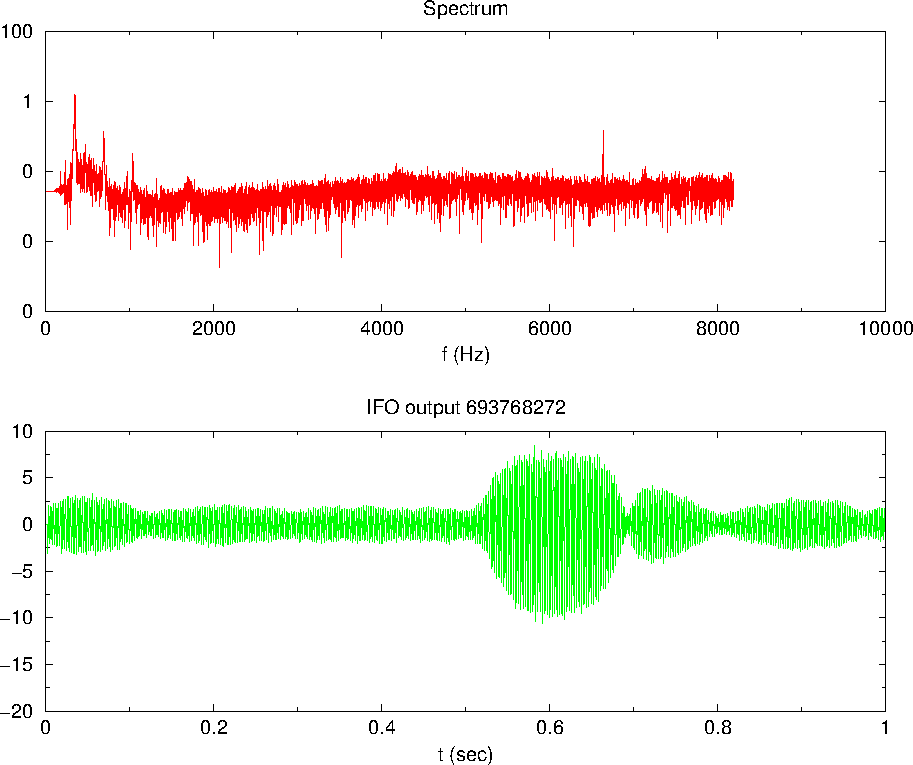
\includegraphics[angle=-90,width=400pt]{animate}
\end{center}
\end{figure}

\item[Author]
Bruce Allen and Patrick Brady

\end{entry}

%%%%%%%%%%%%%%%%%%%%%%%%%%%%%%%%%%%%%%%%%%%%%%%%%%%%%%%%%%%%%%%%%%%%%
%% ZPG2Transfer
%%%%%%%%%%%%%%%%%%%%%%%%%%%%%%%%%%%%%%%%%%%%%%%%%%%%%%%%%%%%%%%%%%%%%
\section{Program \texttt{lalapps\_ZPG2Transfer}}
\label{program:lalapps-ZPG2transfer}
\idx[Program]{lalapps\_ZPG2Transfer}

\begin{entry}

\item[Name]
\verb$lal_ZPG2Transfer$ --- computes transfer function given a
zero-pole-gain representation. 

\item[Synopsis]
\verb$lal_ZPG2Transfer$ [\verb$-z nz z_1 ... z_nz$] [\verb$-p np p_1 .... p_np$] 
                         [\verb$-g gain$] [\verb$-f npoints fmin fmax$] [\verb$-t$]
                         [\verb$-o outfile$] [\verb$-i ilwdfile$]
                         
\item[Description]
\verb$lal_ZPG2Transfer$ computes the frequency domain transfer
function $T(f)$ given a zero-pole-gain representation.   It uses
\verb$LALComputeTransfer()$;  see the LAL Software Documentation under
\texttt{tools} for the definition of the transfer function.

\item[Options]\leavevmode
\begin{entry}
\item[\texttt{-h}]
Print a help message.
\item[\texttt{-z nz z\_1 ... z\_nz}] 
The number of zeros \verb$nz$ followed
by a space and a white space list of \emph{real} zeros specified in units of Hz.
\item[\texttt{-p np p\_1 ... p\_np}] 
The number of zeros \verb$np$ followed
by a space and a white space list of \emph{real} poles specified in units of Hz.
\item[\texttt{-g gain}] 
The gain of the filter.
\item[\texttt{-t}]
If this flag is used,  then the ilwd will indicate units of
counts/attostrain.  The user must correctly choose the zeros, poles,
and gains,  it is not handled automatically.
\item[\texttt{-f npoints fmin fmax}] 
Information about the frequency series.  \verb$npoints$ is the number
of points in the series,  \verb$fmin$ is the lowest frequency to be
represented,  and \verb$fmax$ is the highest frequency to be
represented.   
\item[\texttt{-o} \textit{outfile}]
Write the output to file \textit{outfile} as 3 columns.  Each row
represents the triplet: $\{f,\; \textrm{Re}[T(f)],\; \textrm{Im}[T(f)]\}$.
\item[\texttt{-i} \textit{outfile}]
Write the output to file \textit{outfile} in ILWD format suitable for
ingestion by the datacondAPI in LDAS.
\end{entry}

\item[Example usage]
To compute the transfer function 4 zeros at $0,0,0.74,0.74$Hz,  5
poles at $50.35,50.35,12.1,12.1,186.0$Hz,  and gain $1.47e7$ at 1025
sample points from $0.0$Hz up to $1024.0$Hz and write the ouput as
ILWD:
\begin{verbatim}
./lalapps_ZPG2Transfer -z 4 0.0 0.0 0.74 0.74 \
   -p 5 50.35 50.35 12.1 12.1 186.0 -g 1.47e7 \
   -f 1025 0.0 1024.0 -o response.txt
\end{verbatim}

\item[Author]
Patrick Brady

\end{entry}


%%%%%%%%%%%%%%%%%%%%%%%%%%%%%%%%%%%%%%%%%%%%%%%%%%%%%%%%%%%%%%%%%%%%%
%% BuildTransfer
%%%%%%%%%%%%%%%%%%%%%%%%%%%%%%%%%%%%%%%%%%%%%%%%%%%%%%%%%%%%%%%%%%%%%
\section{Program \texttt{lalapps\_buildTransfer}}
\label{program:lalapps-buildTransfer}
\idx[Program]{lalapps\_buildTransfer}

\begin{entry}

\item[Name]
\verb$lalapps_buildTransfer$ --- computes instrument response function
given a measured swept sine calibration and an overall amplitude
normalization.    

\item[Synopsis]
\verb$lal_buildTransfer$ [\verb$-f npoints fmin fmax$] [\verb$-t$]
                         [\verb$-r outfile$] [\verb$-o outfile$] [\verb$-i ilwdfile$]
                         
\item[Description]
\verb$lal_BuildTransfer$ computes the frequency domain response
function $R(f)$ given a measured swept sine calibration and an overall
amplitude normalization.   

\item[Options]\leavevmode
\begin{entry}
\item[\texttt{-h}]
Print a help message.
\item[\texttt{-r} \textit{infile}]
The input file containing the swept sine calibration.   It should
contain five columns containing frequency, amplitude, error in
amplitude, phase, and error in phase.  See XX for complete
documentation.  
\item[\texttt{-t}]
If this flag is used,  then the ilwd will indicate units of
counts/attostrain.  
\item[\texttt{-f npoints fmin fmax}] 
Information about the frequency series.  \verb$npoints$ is the number
of points in the series,  \verb$fmin$ is the lowest frequency to be
represented,  and \verb$fmax$ is the highest frequency to be
represented.   
\item[\texttt{-o} \textit{outfile}]
Write the output to file \textit{outfile} as 3 columns.  Each row
represents the triplet: $\{f,\; \textrm{Re}[R(f)],\; \textrm{Im}[R(f)]\}$.
\item[\texttt{-i} \textit{outfile}]
Write the output to file \textit{outfile} in ILWD format suitable for
ingestion by the datacondAPI in LDAS.
\end{entry}

\item[Example usage]

To compute the response function from a swept-sine file
\texttt{swept.sine} sample points from $0.0$Hz up to $1024.0$Hz and
write the ouput as ILWD:
\begin{verbatim}
./lalapps_BuildTransfer -z 4 0.0 0.0 0.74 0.74 \
   -p 5 50.35 50.35 12.1 12.1 186.0 -g 1.47e7 \
   -f 1025 0.0 1024.0 -o response.txt
\end{verbatim}

\item[Author]
Patrick Brady

\end{entry}


\chapter{Python DAG/Pipeline Modules}
\label{chapter:python}

\clearpage
%
% API Documentation
% Module pipeline
%
% Generated by epydoc 2.0
% [Wed Sep 24 18:39:38 2003]
%

%%%%%%%%%%%%%%%%%%%%%%%%%%%%%%%%%%%%%%%%%%%%%%%%%%%%%%%%%%%%%%%%%%%%%%%%%%%
%%                          Module Description                           %%
%%%%%%%%%%%%%%%%%%%%%%%%%%%%%%%%%%%%%%%%%%%%%%%%%%%%%%%%%%%%%%%%%%%%%%%%%%%

    \index{pipeline \textit{(module)}|(}
\section{Python Module \texttt{pipeline.py}}

    \label{pipeline}
pipeline.py - condor functions used by pipeline scripts

\$Id$


%%%%%%%%%%%%%%%%%%%%%%%%%%%%%%%%%%%%%%%%%%%%%%%%%%%%%%%%%%%%%%%%%%%%%%%%%%%
%%                               Functions                               %%
%%%%%%%%%%%%%%%%%%%%%%%%%%%%%%%%%%%%%%%%%%%%%%%%%%%%%%%%%%%%%%%%%%%%%%%%%%%

  \subsection{Functions}

    \label{pipeline:s2play}
    \index{pipeline \textit{(module)}!s2play \textit{(function)}}
    \vspace{0.5ex}

    \noindent\begin{boxedminipage}{\textwidth}

    \raggedright \textbf{s2play}(\textit{t})

    \vspace{-1.5ex}

    \rule{\textwidth}{0.5\fboxrule}
    Return 1 if t is in the S2 playground, 0 otherwise t = GPS time to 
    test if playground

    \vspace{1ex}

    \end{boxedminipage}


%%%%%%%%%%%%%%%%%%%%%%%%%%%%%%%%%%%%%%%%%%%%%%%%%%%%%%%%%%%%%%%%%%%%%%%%%%%
%%                               Variables                               %%
%%%%%%%%%%%%%%%%%%%%%%%%%%%%%%%%%%%%%%%%%%%%%%%%%%%%%%%%%%%%%%%%%%%%%%%%%%%

  \subsection{Variables}

\begin{longtable}{|p{.30\textwidth}|p{.62\textwidth}|l}
\cline{1-2}
\cline{1-2} \centering \textbf{Name} & \centering \textbf{Description}& \\
\cline{1-2}
\endhead\cline{1-2}\multicolumn{3}{r}{\small\textit{continued on next page}}\\\endfoot\cline{1-2}
\endlastfoot\raggedright \_\-\_\-a\-u\-t\-h\-o\-r\-\_\-\_\- & \raggedright \textbf{Value:} 
{\tt '\-D\-u\-n\-c\-a\-n\-~\-B\-r\-o\-w\-n\-~\-{\textless}\-d\-u\-n\-c\-a\-n\-@\-g\-r\-a\-v\-i\-t\-y\-.\-p\-h\-y\-s\-.\-u\-w\-m\-.\-e\-d\-u\-{\textgreater}\-'\-}&\\
\cline{1-2}
\raggedright \_\-\_\-d\-a\-t\-e\-\_\-\_\- & \raggedright \textbf{Value:} 
{\tt '\-\$\-D\-a\-t\-e\-:\-~\-2\-0\-0\-3\-/\-0\-9\-/\-2\-3\-~\-1\-6\-:\-3\-3\-:\-4\-6\-~\-\$\-'\-}&\\
\cline{1-2}
\raggedright \_\-\_\-v\-e\-r\-s\-i\-o\-n\-\_\-\_\- & \raggedright \textbf{Value:} 
{\tt '\-1\-.\-2\-'\-}&\\
\cline{1-2}
\end{longtable}

    \index{pipeline \textit{(module)}!AnalysisChunk \textit{(class)}|(}

%%%%%%%%%%%%%%%%%%%%%%%%%%%%%%%%%%%%%%%%%%%%%%%%%%%%%%%%%%%%%%%%%%%%%%%%%%%
%%                           Class Description                           %%
%%%%%%%%%%%%%%%%%%%%%%%%%%%%%%%%%%%%%%%%%%%%%%%%%%%%%%%%%%%%%%%%%%%%%%%%%%%

\subsection{Class AnalysisChunk}

    \label{pipeline:AnalysisChunk}
An AnalysisCunk is the unit of data that a node works with, usually some 
subset of a ScienceSegment.


%%%%%%%%%%%%%%%%%%%%%%%%%%%%%%%%%%%%%%%%%%%%%%%%%%%%%%%%%%%%%%%%%%%%%%%%%%%
%%                                Methods                                %%
%%%%%%%%%%%%%%%%%%%%%%%%%%%%%%%%%%%%%%%%%%%%%%%%%%%%%%%%%%%%%%%%%%%%%%%%%%%

  \subsubsection{Methods}

    \label{pipeline:AnalysisChunk:__init__}
    \index{pipeline \textit{(module)}!AnalysisChunk \textit{(class)}!\_\_init\_\_ \textit{(method)}}
    \vspace{0.5ex}

    \noindent\begin{boxedminipage}{\textwidth}

    \raggedright \textbf{\_\_init\_\_}(\textit{self}, \textit{start}, \textit{end})

    \vspace{-1.5ex}

    \rule{\textwidth}{0.5\fboxrule}
    start = GPS start time of the chunk. end = GPS end time of the chunk.

    \vspace{1ex}

    \end{boxedminipage}

    \label{pipeline:AnalysisChunk:__repr__}
    \index{pipeline \textit{(module)}!AnalysisChunk \textit{(class)}!\_\_repr\_\_ \textit{(method)}}
    \vspace{0.5ex}

    \noindent\begin{boxedminipage}{\textwidth}

    \raggedright \textbf{\_\_repr\_\_}(\textit{self})

    \end{boxedminipage}

    \label{pipeline:AnalysisChunk:dur}
    \index{pipeline \textit{(module)}!AnalysisChunk \textit{(class)}!dur \textit{(method)}}
    \vspace{0.5ex}

    \noindent\begin{boxedminipage}{\textwidth}

    \raggedright \textbf{dur}(\textit{self})

    \vspace{-1.5ex}

    \rule{\textwidth}{0.5\fboxrule}
    Returns the length (duration) of the chunk in seconds.

    \vspace{1ex}

    \end{boxedminipage}

    \label{pipeline:AnalysisChunk:end}
    \index{pipeline \textit{(module)}!AnalysisChunk \textit{(class)}!end \textit{(method)}}
    \vspace{0.5ex}

    \noindent\begin{boxedminipage}{\textwidth}

    \raggedright \textbf{end}(\textit{self})

    \vspace{-1.5ex}

    \rule{\textwidth}{0.5\fboxrule}
    Returns the GPS end time of the chunk.

    \vspace{1ex}

    \end{boxedminipage}

    \label{pipeline:AnalysisChunk:start}
    \index{pipeline \textit{(module)}!AnalysisChunk \textit{(class)}!start \textit{(method)}}
    \vspace{0.5ex}

    \noindent\begin{boxedminipage}{\textwidth}

    \raggedright \textbf{start}(\textit{self})

    \vspace{-1.5ex}

    \rule{\textwidth}{0.5\fboxrule}
    Returns the GPS start time of the chunk.

    \vspace{1ex}

    \end{boxedminipage}

    \index{pipeline \textit{(module)}!AnalysisChunk \textit{(class)}|)}
    \index{pipeline \textit{(module)}!AnalysisJob \textit{(class)}|(}

%%%%%%%%%%%%%%%%%%%%%%%%%%%%%%%%%%%%%%%%%%%%%%%%%%%%%%%%%%%%%%%%%%%%%%%%%%%
%%                           Class Description                           %%
%%%%%%%%%%%%%%%%%%%%%%%%%%%%%%%%%%%%%%%%%%%%%%%%%%%%%%%%%%%%%%%%%%%%%%%%%%%

\subsection{Class AnalysisJob}

    \label{pipeline:AnalysisJob}
Describes a generic analysis job that filters LIGO data as configured by 
an ini file.


%%%%%%%%%%%%%%%%%%%%%%%%%%%%%%%%%%%%%%%%%%%%%%%%%%%%%%%%%%%%%%%%%%%%%%%%%%%
%%                                Methods                                %%
%%%%%%%%%%%%%%%%%%%%%%%%%%%%%%%%%%%%%%%%%%%%%%%%%%%%%%%%%%%%%%%%%%%%%%%%%%%

  \subsubsection{Methods}

    \label{pipeline:AnalysisJob:__init__}
    \index{pipeline \textit{(module)}!AnalysisJob \textit{(class)}!\_\_init\_\_ \textit{(method)}}
    \vspace{0.5ex}

    \noindent\begin{boxedminipage}{\textwidth}

    \raggedright \textbf{\_\_init\_\_}(\textit{self}, \textit{cp})

    \vspace{-1.5ex}

    \rule{\textwidth}{0.5\fboxrule}
    cp = ConfigParser object that contains the configuration for this 
    job.

    \vspace{1ex}

    \end{boxedminipage}

    \label{pipeline:AnalysisJob:calibration}
    \index{pipeline \textit{(module)}!AnalysisJob \textit{(class)}!calibration \textit{(method)}}
    \vspace{0.5ex}

    \noindent\begin{boxedminipage}{\textwidth}

    \raggedright \textbf{calibration}(\textit{self}, \textit{ifo})

    \vspace{-1.5ex}

    \rule{\textwidth}{0.5\fboxrule}
    Returns the name of the calibration file to use for the given IFO. 
    ifo = name of interferomener (e.g. L1, H1 or H2).

    \vspace{1ex}

    \end{boxedminipage}

    \label{pipeline:AnalysisJob:channel}
    \index{pipeline \textit{(module)}!AnalysisJob \textit{(class)}!channel \textit{(method)}}
    \vspace{0.5ex}

    \noindent\begin{boxedminipage}{\textwidth}

    \raggedright \textbf{channel}(\textit{self})

    \vspace{-1.5ex}

    \rule{\textwidth}{0.5\fboxrule}
    Returns the name of the channel that this job is filtering. Note that 
    channel is defined to be IFO independent, so this may be LSC-AS\_Q or 
    IOO-MC\_F. The IFO is set on a per node basis, not a per job basis.

    \vspace{1ex}

    \end{boxedminipage}

    \label{pipeline:AnalysisJob:get_config}
    \index{pipeline \textit{(module)}!AnalysisJob \textit{(class)}!get\_config \textit{(method)}}
    \vspace{0.5ex}

    \noindent\begin{boxedminipage}{\textwidth}

    \raggedright \textbf{get\_config}(\textit{self}, \textit{sec}, \textit{opt})

    \vspace{-1.5ex}

    \rule{\textwidth}{0.5\fboxrule}
    Get the configration variable in a particular section of this jobs 
    ini file. sec = ini file section. opt = option from section sec.

    \vspace{1ex}

    \end{boxedminipage}

    \index{pipeline \textit{(module)}!AnalysisJob \textit{(class)}|)}
    \index{pipeline \textit{(module)}!AnalysisNode \textit{(class)}|(}

%%%%%%%%%%%%%%%%%%%%%%%%%%%%%%%%%%%%%%%%%%%%%%%%%%%%%%%%%%%%%%%%%%%%%%%%%%%
%%                           Class Description                           %%
%%%%%%%%%%%%%%%%%%%%%%%%%%%%%%%%%%%%%%%%%%%%%%%%%%%%%%%%%%%%%%%%%%%%%%%%%%%

\subsection{Class AnalysisNode}

    \label{pipeline:AnalysisNode}
\begin{tabular}{cccccc}
% Line for pipeline.CondorDAGNode, linespec=[0]
\multicolumn{2}{r}{\settowidth{\BCL}{pipeline.CondorDAGNode}\multirow{2}{\BCL}{pipeline.CondorDAGNode}}
&&
  \\\cline{3-3}
  &&\multicolumn{1}{c|}{}
&&
  \\
&&\multicolumn{2}{l}{\textbf{AnalysisNode}}
\end{tabular}

Contains the methods that allow an object to be built to analyse LIGO 
data in a Condor DAG.


%%%%%%%%%%%%%%%%%%%%%%%%%%%%%%%%%%%%%%%%%%%%%%%%%%%%%%%%%%%%%%%%%%%%%%%%%%%
%%                                Methods                                %%
%%%%%%%%%%%%%%%%%%%%%%%%%%%%%%%%%%%%%%%%%%%%%%%%%%%%%%%%%%%%%%%%%%%%%%%%%%%

  \subsubsection{Methods}

    \label{pipeline:AnalysisNode:__init__}
    \index{pipeline \textit{(module)}!AnalysisNode \textit{(class)}!\_\_init\_\_ \textit{(method)}}
    \vspace{0.5ex}

    \noindent\begin{boxedminipage}{\textwidth}

    \raggedright \textbf{\_\_init\_\_}(\textit{self})

      Overrides: pipeline.CondorDAGNode.\_\_init\_\_

    \end{boxedminipage}

    \label{pipeline:AnalysisNode:get_end}
    \index{pipeline \textit{(module)}!AnalysisNode \textit{(class)}!get\_end \textit{(method)}}
    \vspace{0.5ex}

    \noindent\begin{boxedminipage}{\textwidth}

    \raggedright \textbf{get\_end}(\textit{self})

    \vspace{-1.5ex}

    \rule{\textwidth}{0.5\fboxrule}
    Get the GPS end time of the node.

    \vspace{1ex}

    \end{boxedminipage}

    \label{pipeline:AnalysisNode:get_ifo}
    \index{pipeline \textit{(module)}!AnalysisNode \textit{(class)}!get\_ifo \textit{(method)}}
    \vspace{0.5ex}

    \noindent\begin{boxedminipage}{\textwidth}

    \raggedright \textbf{get\_ifo}(\textit{self})

    \vspace{-1.5ex}

    \rule{\textwidth}{0.5\fboxrule}
    Returns the two letter IFO code for this node.

    \vspace{1ex}

    \end{boxedminipage}

    \label{pipeline:AnalysisNode:get_input}
    \index{pipeline \textit{(module)}!AnalysisNode \textit{(class)}!get\_input \textit{(method)}}
    \vspace{0.5ex}

    \noindent\begin{boxedminipage}{\textwidth}

    \raggedright \textbf{get\_input}(\textit{self})

    \vspace{-1.5ex}

    \rule{\textwidth}{0.5\fboxrule}
    Get the file that will be passed as input.

    \vspace{1ex}

    \end{boxedminipage}

    \label{pipeline:AnalysisNode:get_output}
    \index{pipeline \textit{(module)}!AnalysisNode \textit{(class)}!get\_output \textit{(method)}}
    \vspace{0.5ex}

    \noindent\begin{boxedminipage}{\textwidth}

    \raggedright \textbf{get\_output}(\textit{self})

    \vspace{-1.5ex}

    \rule{\textwidth}{0.5\fboxrule}
    Get the file that will be passed as output.

    \vspace{1ex}

    \end{boxedminipage}

    \label{pipeline:AnalysisNode:get_start}
    \index{pipeline \textit{(module)}!AnalysisNode \textit{(class)}!get\_start \textit{(method)}}
    \vspace{0.5ex}

    \noindent\begin{boxedminipage}{\textwidth}

    \raggedright \textbf{get\_start}(\textit{self})

    \vspace{-1.5ex}

    \rule{\textwidth}{0.5\fboxrule}
    Get the GPS start time of the node.

    \vspace{1ex}

    \end{boxedminipage}

    \label{pipeline:AnalysisNode:set_cache}
    \index{pipeline \textit{(module)}!AnalysisNode \textit{(class)}!set\_cache \textit{(method)}}
    \vspace{0.5ex}

    \noindent\begin{boxedminipage}{\textwidth}

    \raggedright \textbf{set\_cache}(\textit{self}, \textit{file})

    \vspace{-1.5ex}

    \rule{\textwidth}{0.5\fboxrule}
    Set the LAL frame cache to to use. The frame cache is passed to the 
    job with the --frame-cache argument. file = calibration file to use.

    \vspace{1ex}

    \end{boxedminipage}

    \label{pipeline:AnalysisNode:set_end}
    \index{pipeline \textit{(module)}!AnalysisNode \textit{(class)}!set\_end \textit{(method)}}
    \vspace{0.5ex}

    \noindent\begin{boxedminipage}{\textwidth}

    \raggedright \textbf{set\_end}(\textit{self}, \textit{time})

    \vspace{-1.5ex}

    \rule{\textwidth}{0.5\fboxrule}
    Set the GPS end time of the analysis node by setting a --gps-end-time 
    option to the node when it is executed. time = GPS end time of job.

    \vspace{1ex}

    \end{boxedminipage}

    \label{pipeline:AnalysisNode:set_ifo}
    \index{pipeline \textit{(module)}!AnalysisNode \textit{(class)}!set\_ifo \textit{(method)}}
    \vspace{0.5ex}

    \noindent\begin{boxedminipage}{\textwidth}

    \raggedright \textbf{set\_ifo}(\textit{self}, \textit{ifo})

    \vspace{-1.5ex}

    \rule{\textwidth}{0.5\fboxrule}
    Set the channel name to analyze and add a calibration file for that 
    channel. The name of the ifo is prepended to the channel name 
    obtained from the job configuration file and passed with a 
    --channel-name option. A calibration file is obtained from the ini 
    file and passed with a --calibration-cache option. ifo = two letter 
    ifo code (e.g. L1, H1 or H2).

    \vspace{1ex}

    \end{boxedminipage}

    \label{pipeline:AnalysisNode:set_input}
    \index{pipeline \textit{(module)}!AnalysisNode \textit{(class)}!set\_input \textit{(method)}}
    \vspace{0.5ex}

    \noindent\begin{boxedminipage}{\textwidth}

    \raggedright \textbf{set\_input}(\textit{self}, \textit{file})

    \vspace{-1.5ex}

    \rule{\textwidth}{0.5\fboxrule}
    Add an input to the node by adding a --input option. file = option 
    argument to pass as input.

    \vspace{1ex}

    \end{boxedminipage}

    \label{pipeline:AnalysisNode:set_output}
    \index{pipeline \textit{(module)}!AnalysisNode \textit{(class)}!set\_output \textit{(method)}}
    \vspace{0.5ex}

    \noindent\begin{boxedminipage}{\textwidth}

    \raggedright \textbf{set\_output}(\textit{self}, \textit{file})

    \vspace{-1.5ex}

    \rule{\textwidth}{0.5\fboxrule}
    Add an output to the node by adding a --output option. file = option 
    argument to pass as output.

    \vspace{1ex}

    \end{boxedminipage}

    \label{pipeline:AnalysisNode:set_start}
    \index{pipeline \textit{(module)}!AnalysisNode \textit{(class)}!set\_start \textit{(method)}}
    \vspace{0.5ex}

    \noindent\begin{boxedminipage}{\textwidth}

    \raggedright \textbf{set\_start}(\textit{self}, \textit{time})

    \vspace{-1.5ex}

    \rule{\textwidth}{0.5\fboxrule}
    Set the GPS start time of the analysis node by setting a 
    --gps-start-time option to the node when it is executed. time = GPS 
    start time of job.

    \vspace{1ex}

    \end{boxedminipage}

  \textbf{Inherited from CondorDAGNode:}
    \_\_repr\_\_,
    add\_parent,
    add\_var,
    job,
    set\_log\_file,
    set\_name,
    set\_retry,
    write
    \index{pipeline \textit{(module)}!AnalysisNode \textit{(class)}|)}
    \index{pipeline \textit{(module)}!CondorDAG \textit{(class)}|(}

%%%%%%%%%%%%%%%%%%%%%%%%%%%%%%%%%%%%%%%%%%%%%%%%%%%%%%%%%%%%%%%%%%%%%%%%%%%
%%                           Class Description                           %%
%%%%%%%%%%%%%%%%%%%%%%%%%%%%%%%%%%%%%%%%%%%%%%%%%%%%%%%%%%%%%%%%%%%%%%%%%%%

\subsection{Class CondorDAG}

    \label{pipeline:CondorDAG}
A CondorDAG is a Condor Directed Acyclic Graph that describes a 
collection of Condor jobs and the order in which to run them. All Condor 
jobs in the DAG must write their Codor logs to the same file. NOTE: The 
log file must not be on an NFS mounted system as the Condor jobs must be 
able to get an exclusive file lock on the log file.


%%%%%%%%%%%%%%%%%%%%%%%%%%%%%%%%%%%%%%%%%%%%%%%%%%%%%%%%%%%%%%%%%%%%%%%%%%%
%%                                Methods                                %%
%%%%%%%%%%%%%%%%%%%%%%%%%%%%%%%%%%%%%%%%%%%%%%%%%%%%%%%%%%%%%%%%%%%%%%%%%%%

  \subsubsection{Methods}

    \label{pipeline:CondorDAG:__init__}
    \index{pipeline \textit{(module)}!CondorDAG \textit{(class)}!\_\_init\_\_ \textit{(method)}}
    \vspace{0.5ex}

    \noindent\begin{boxedminipage}{\textwidth}

    \raggedright \textbf{\_\_init\_\_}(\textit{self}, \textit{log})

    \vspace{-1.5ex}

    \rule{\textwidth}{0.5\fboxrule}
    log = path to log file which must not be on an NFS mounted file 
    system.

    \vspace{1ex}

    \end{boxedminipage}

    \label{pipeline:CondorDAG:add_node}
    \index{pipeline \textit{(module)}!CondorDAG \textit{(class)}!add\_node \textit{(method)}}
    \vspace{0.5ex}

    \noindent\begin{boxedminipage}{\textwidth}

    \raggedright \textbf{add\_node}(\textit{self}, \textit{node})

    \vspace{-1.5ex}

    \rule{\textwidth}{0.5\fboxrule}
    Add a CondorDAGNode to this DAG. The CondorJob that the node uses is 
    also added to the list of Condor jobs in the DAG so that a list of 
    the submit files needed by the DAG can be maintained. Each unique 
    CondorJob will be added once to prevent duplicate submit files being 
    written. node = CondorDAGNode to add to the CondorDAG.

    \vspace{1ex}

    \end{boxedminipage}

    \label{pipeline:CondorDAG:set_dag_file}
    \index{pipeline \textit{(module)}!CondorDAG \textit{(class)}!set\_dag\_file \textit{(method)}}
    \vspace{0.5ex}

    \noindent\begin{boxedminipage}{\textwidth}

    \raggedright \textbf{set\_dag\_file}(\textit{self}, \textit{path})

    \vspace{-1.5ex}

    \rule{\textwidth}{0.5\fboxrule}
    Set the name of the file into which the DAG is written. path = path 
    to DAG file.

    \vspace{1ex}

    \end{boxedminipage}

    \label{pipeline:CondorDAG:write_dag}
    \index{pipeline \textit{(module)}!CondorDAG \textit{(class)}!write\_dag \textit{(method)}}
    \vspace{0.5ex}

    \noindent\begin{boxedminipage}{\textwidth}

    \raggedright \textbf{write\_dag}(\textit{self})

    \vspace{-1.5ex}

    \rule{\textwidth}{0.5\fboxrule}
    Write all the nodes in the DAG to the DAG file.

    \vspace{1ex}

    \end{boxedminipage}

    \label{pipeline:CondorDAG:write_sub_files}
    \index{pipeline \textit{(module)}!CondorDAG \textit{(class)}!write\_sub\_files \textit{(method)}}
    \vspace{0.5ex}

    \noindent\begin{boxedminipage}{\textwidth}

    \raggedright \textbf{write\_sub\_files}(\textit{self})

    \vspace{-1.5ex}

    \rule{\textwidth}{0.5\fboxrule}
    Write all the submit files used by the dag to disk. Each submit file 
    is written to the file name set in the CondorJob.

    \vspace{1ex}

    \end{boxedminipage}

    \index{pipeline \textit{(module)}!CondorDAG \textit{(class)}|)}
    \index{pipeline \textit{(module)}!CondorDAGError \textit{(class)}|(}

%%%%%%%%%%%%%%%%%%%%%%%%%%%%%%%%%%%%%%%%%%%%%%%%%%%%%%%%%%%%%%%%%%%%%%%%%%%
%%                           Class Description                           %%
%%%%%%%%%%%%%%%%%%%%%%%%%%%%%%%%%%%%%%%%%%%%%%%%%%%%%%%%%%%%%%%%%%%%%%%%%%%

\subsection{Class CondorDAGError}

    \label{pipeline:CondorDAGError}
\begin{tabular}{cccccccc}
% Line for exceptions.Exception, linespec=[0, 0]
\multicolumn{2}{r}{\settowidth{\BCL}{exceptions.Exception}\multirow{2}{\BCL}{exceptions.Exception}}
&&
&&
  \\\cline{3-3}
  &&\multicolumn{1}{c|}{}
&&
&&
  \\
% Line for pipeline.CondorError, linespec=[0]
\multicolumn{4}{r}{\settowidth{\BCL}{pipeline.CondorError}\multirow{2}{\BCL}{pipeline.CondorError}}
&&
  \\\cline{5-5}
  &&&&\multicolumn{1}{c|}{}
&&
  \\
&&&&\multicolumn{2}{l}{\textbf{CondorDAGError}}
\end{tabular}


%%%%%%%%%%%%%%%%%%%%%%%%%%%%%%%%%%%%%%%%%%%%%%%%%%%%%%%%%%%%%%%%%%%%%%%%%%%
%%                                Methods                                %%
%%%%%%%%%%%%%%%%%%%%%%%%%%%%%%%%%%%%%%%%%%%%%%%%%%%%%%%%%%%%%%%%%%%%%%%%%%%

  \subsubsection{Methods}

  \textbf{Inherited from Exception:}
    \_\_getitem\_\_,
    \_\_str\_\_
    \\
  \textbf{Inherited from CondorError:}
    \_\_init\_\_
    \index{pipeline \textit{(module)}!CondorDAGError \textit{(class)}|)}
    \index{pipeline \textit{(module)}!CondorDAGJob \textit{(class)}|(}

%%%%%%%%%%%%%%%%%%%%%%%%%%%%%%%%%%%%%%%%%%%%%%%%%%%%%%%%%%%%%%%%%%%%%%%%%%%
%%                           Class Description                           %%
%%%%%%%%%%%%%%%%%%%%%%%%%%%%%%%%%%%%%%%%%%%%%%%%%%%%%%%%%%%%%%%%%%%%%%%%%%%

\subsection{Class CondorDAGJob}

    \label{pipeline:CondorDAGJob}
\begin{tabular}{cccccc}
% Line for pipeline.CondorJob, linespec=[0]
\multicolumn{2}{r}{\settowidth{\BCL}{pipeline.CondorJob}\multirow{2}{\BCL}{pipeline.CondorJob}}
&&
  \\\cline{3-3}
  &&\multicolumn{1}{c|}{}
&&
  \\
&&\multicolumn{2}{l}{\textbf{CondorDAGJob}}
\end{tabular}

A Condor DAG job never notifies the user on completion and can have 
variable arguments that are set for a particular node in the DAG. 
Inherits methods from a CondorJob.


%%%%%%%%%%%%%%%%%%%%%%%%%%%%%%%%%%%%%%%%%%%%%%%%%%%%%%%%%%%%%%%%%%%%%%%%%%%
%%                                Methods                                %%
%%%%%%%%%%%%%%%%%%%%%%%%%%%%%%%%%%%%%%%%%%%%%%%%%%%%%%%%%%%%%%%%%%%%%%%%%%%

  \subsubsection{Methods}

    \label{pipeline:CondorDAGJob:__init__}
    \index{pipeline \textit{(module)}!CondorDAGJob \textit{(class)}!\_\_init\_\_ \textit{(method)}}
    \vspace{0.5ex}

    \noindent\begin{boxedminipage}{\textwidth}

    \raggedright \textbf{\_\_init\_\_}(\textit{self}, \textit{universe}, \textit{executable})

    \vspace{-1.5ex}

    \rule{\textwidth}{0.5\fboxrule}
    universe = the condor universe to run the job in. executable = the 
    executable to run in the DAG.

    \vspace{1ex}

      Overrides: pipeline.CondorJob.\_\_init\_\_

    \end{boxedminipage}

    \label{pipeline:CondorDAGJob:add_var_arg}
    \index{pipeline \textit{(module)}!CondorDAGJob \textit{(class)}!add\_var\_arg \textit{(method)}}
    \vspace{0.5ex}

    \noindent\begin{boxedminipage}{\textwidth}

    \raggedright \textbf{add\_var\_arg}(\textit{self}, \textit{arg})

    \vspace{-1.5ex}

    \rule{\textwidth}{0.5\fboxrule}
    Add a variable (or macro) option to the condor job. The option is 
    added to the submit file and a different argument to the option can 
    be set fot each node in the DAG. arg = name of option to add.

    \vspace{1ex}

    \end{boxedminipage}

  \textbf{Inherited from CondorJob:}
    add\_arg,
    add\_ini\_args,
    get\_stderr\_file,
    get\_stdout\_file,
    get\_sub\_file,
    set\_log\_file,
    set\_notifcation,
    set\_stderr\_file,
    set\_stdout\_file,
    set\_sub\_file,
    write\_sub\_file
    \index{pipeline \textit{(module)}!CondorDAGJob \textit{(class)}|)}
    \index{pipeline \textit{(module)}!CondorDAGNode \textit{(class)}|(}

%%%%%%%%%%%%%%%%%%%%%%%%%%%%%%%%%%%%%%%%%%%%%%%%%%%%%%%%%%%%%%%%%%%%%%%%%%%
%%                           Class Description                           %%
%%%%%%%%%%%%%%%%%%%%%%%%%%%%%%%%%%%%%%%%%%%%%%%%%%%%%%%%%%%%%%%%%%%%%%%%%%%

\subsection{Class CondorDAGNode}

    \label{pipeline:CondorDAGNode}
\textbf{Known Subclasses:} AnalysisNode

A CondorDAGNode represents a node in the DAG. It corresponds to a 
particular condor job (and so a particular submit file). If the job has 
variable (macro) arguments, they can be set here so each nodes executes 
with the correct arguments.


%%%%%%%%%%%%%%%%%%%%%%%%%%%%%%%%%%%%%%%%%%%%%%%%%%%%%%%%%%%%%%%%%%%%%%%%%%%
%%                                Methods                                %%
%%%%%%%%%%%%%%%%%%%%%%%%%%%%%%%%%%%%%%%%%%%%%%%%%%%%%%%%%%%%%%%%%%%%%%%%%%%

  \subsubsection{Methods}

    \label{pipeline:CondorDAGNode:__init__}
    \index{pipeline \textit{(module)}!CondorDAGNode \textit{(class)}!\_\_init\_\_ \textit{(method)}}
    \vspace{0.5ex}

    \noindent\begin{boxedminipage}{\textwidth}

    \raggedright \textbf{\_\_init\_\_}(\textit{self}, \textit{job})

    \vspace{-1.5ex}

    \rule{\textwidth}{0.5\fboxrule}
    job = the CondorJob that this node corresponds to.

    \vspace{1ex}

    \end{boxedminipage}

    \label{pipeline:CondorDAGNode:__repr__}
    \index{pipeline \textit{(module)}!CondorDAGNode \textit{(class)}!\_\_repr\_\_ \textit{(method)}}
    \vspace{0.5ex}

    \noindent\begin{boxedminipage}{\textwidth}

    \raggedright \textbf{\_\_repr\_\_}(\textit{self})

    \end{boxedminipage}

    \label{pipeline:CondorDAGNode:add_parent}
    \index{pipeline \textit{(module)}!CondorDAGNode \textit{(class)}!add\_parent \textit{(method)}}
    \vspace{0.5ex}

    \noindent\begin{boxedminipage}{\textwidth}

    \raggedright \textbf{add\_parent}(\textit{self}, \textit{node})

    \vspace{-1.5ex}

    \rule{\textwidth}{0.5\fboxrule}
    Add a parent to this node. This node will not be executed until the 
    parent node has run sucessfully. node = CondorDAGNode to add as a 
    parent.

    \vspace{1ex}

    \end{boxedminipage}

    \label{pipeline:CondorDAGNode:add_var}
    \index{pipeline \textit{(module)}!CondorDAGNode \textit{(class)}!add\_var \textit{(method)}}
    \vspace{0.5ex}

    \noindent\begin{boxedminipage}{\textwidth}

    \raggedright \textbf{add\_var}(\textit{self}, \textit{var}, \textit{value})

    \vspace{-1.5ex}

    \rule{\textwidth}{0.5\fboxrule}
    Add the a variable (macro) arguments for this node. If the option 
    specified does not exist in the CondorJob, it is added so the submit 
    file will be correct when written. var = option name. value = value 
    of the option for this node in the DAG.

    \vspace{1ex}

    \end{boxedminipage}

    \label{pipeline:CondorDAGNode:job}
    \index{pipeline \textit{(module)}!CondorDAGNode \textit{(class)}!job \textit{(method)}}
    \vspace{0.5ex}

    \noindent\begin{boxedminipage}{\textwidth}

    \raggedright \textbf{job}(\textit{self})

    \vspace{-1.5ex}

    \rule{\textwidth}{0.5\fboxrule}
    Return the CondorJob that this node is associated with.

    \vspace{1ex}

    \end{boxedminipage}

    \label{pipeline:CondorDAGNode:set_log_file}
    \index{pipeline \textit{(module)}!CondorDAGNode \textit{(class)}!set\_log\_file \textit{(method)}}
    \vspace{0.5ex}

    \noindent\begin{boxedminipage}{\textwidth}

    \raggedright \textbf{set\_log\_file}(\textit{self}, \textit{log})

    \vspace{-1.5ex}

    \rule{\textwidth}{0.5\fboxrule}
    Set the Condor log file to be used by this CondorJob. log = path of 
    Condor log file.

    \vspace{1ex}

    \end{boxedminipage}

    \label{pipeline:CondorDAGNode:set_name}
    \index{pipeline \textit{(module)}!CondorDAGNode \textit{(class)}!set\_name \textit{(method)}}
    \vspace{0.5ex}

    \noindent\begin{boxedminipage}{\textwidth}

    \raggedright \textbf{set\_name}(\textit{self})

    \vspace{-1.5ex}

    \rule{\textwidth}{0.5\fboxrule}
    Generate a unique name for this node in the DAG.

    \vspace{1ex}

    \end{boxedminipage}

    \label{pipeline:CondorDAGNode:set_retry}
    \index{pipeline \textit{(module)}!CondorDAGNode \textit{(class)}!set\_retry \textit{(method)}}
    \vspace{0.5ex}

    \noindent\begin{boxedminipage}{\textwidth}

    \raggedright \textbf{set\_retry}(\textit{self}, \textit{retry})

    \vspace{-1.5ex}

    \rule{\textwidth}{0.5\fboxrule}
    Set the number of times that this node in the DAG should retry. retry 
    = number of times to retry node.

    \vspace{1ex}

    \end{boxedminipage}

    \label{pipeline:CondorDAGNode:write}
    \index{pipeline \textit{(module)}!CondorDAGNode \textit{(class)}!write \textit{(method)}}
    \vspace{0.5ex}

    \noindent\begin{boxedminipage}{\textwidth}

    \raggedright \textbf{write}(\textit{self}, \textit{fh})

    \vspace{-1.5ex}

    \rule{\textwidth}{0.5\fboxrule}
    Write the DAG entry for this node to the DAG file descriptor. fh = 
    descriptor of open DAG file.

    \vspace{1ex}

    \end{boxedminipage}

    \index{pipeline \textit{(module)}!CondorDAGNode \textit{(class)}|)}
    \index{pipeline \textit{(module)}!CondorDAGNodeError \textit{(class)}|(}

%%%%%%%%%%%%%%%%%%%%%%%%%%%%%%%%%%%%%%%%%%%%%%%%%%%%%%%%%%%%%%%%%%%%%%%%%%%
%%                           Class Description                           %%
%%%%%%%%%%%%%%%%%%%%%%%%%%%%%%%%%%%%%%%%%%%%%%%%%%%%%%%%%%%%%%%%%%%%%%%%%%%

\subsection{Class CondorDAGNodeError}

    \label{pipeline:CondorDAGNodeError}
\begin{tabular}{cccccccc}
% Line for exceptions.Exception, linespec=[0, 0]
\multicolumn{2}{r}{\settowidth{\BCL}{exceptions.Exception}\multirow{2}{\BCL}{exceptions.Exception}}
&&
&&
  \\\cline{3-3}
  &&\multicolumn{1}{c|}{}
&&
&&
  \\
% Line for pipeline.CondorError, linespec=[0]
\multicolumn{4}{r}{\settowidth{\BCL}{pipeline.CondorError}\multirow{2}{\BCL}{pipeline.CondorError}}
&&
  \\\cline{5-5}
  &&&&\multicolumn{1}{c|}{}
&&
  \\
&&&&\multicolumn{2}{l}{\textbf{CondorDAGNodeError}}
\end{tabular}


%%%%%%%%%%%%%%%%%%%%%%%%%%%%%%%%%%%%%%%%%%%%%%%%%%%%%%%%%%%%%%%%%%%%%%%%%%%
%%                                Methods                                %%
%%%%%%%%%%%%%%%%%%%%%%%%%%%%%%%%%%%%%%%%%%%%%%%%%%%%%%%%%%%%%%%%%%%%%%%%%%%

  \subsubsection{Methods}

  \textbf{Inherited from Exception:}
    \_\_getitem\_\_,
    \_\_str\_\_
    \\
  \textbf{Inherited from CondorError:}
    \_\_init\_\_
    \index{pipeline \textit{(module)}!CondorDAGNodeError \textit{(class)}|)}
    \index{pipeline \textit{(module)}!CondorError \textit{(class)}|(}

%%%%%%%%%%%%%%%%%%%%%%%%%%%%%%%%%%%%%%%%%%%%%%%%%%%%%%%%%%%%%%%%%%%%%%%%%%%
%%                           Class Description                           %%
%%%%%%%%%%%%%%%%%%%%%%%%%%%%%%%%%%%%%%%%%%%%%%%%%%%%%%%%%%%%%%%%%%%%%%%%%%%

\subsection{Class CondorError}

    \label{pipeline:CondorError}
\begin{tabular}{cccccc}
% Line for exceptions.Exception, linespec=[0]
\multicolumn{2}{r}{\settowidth{\BCL}{exceptions.Exception}\multirow{2}{\BCL}{exceptions.Exception}}
&&
  \\\cline{3-3}
  &&\multicolumn{1}{c|}{}
&&
  \\
&&\multicolumn{2}{l}{\textbf{CondorError}}
\end{tabular}

\textbf{Known Subclasses:}
CondorDAGError,
    CondorDAGNodeError,
    CondorJobError,
    CondorSubmitError

Error thrown by Condor Jobs


%%%%%%%%%%%%%%%%%%%%%%%%%%%%%%%%%%%%%%%%%%%%%%%%%%%%%%%%%%%%%%%%%%%%%%%%%%%
%%                                Methods                                %%
%%%%%%%%%%%%%%%%%%%%%%%%%%%%%%%%%%%%%%%%%%%%%%%%%%%%%%%%%%%%%%%%%%%%%%%%%%%

  \subsubsection{Methods}

    \label{pipeline:CondorError:__init__}
    \index{pipeline \textit{(module)}!CondorError \textit{(class)}!\_\_init\_\_ \textit{(method)}}
    \vspace{0.5ex}

    \noindent\begin{boxedminipage}{\textwidth}

    \raggedright \textbf{\_\_init\_\_}(\textit{self}, \textit{args}=\texttt{N\-o\-n\-e\-})

      Overrides: exceptions.Exception.\_\_init\_\_

    \end{boxedminipage}

  \textbf{Inherited from Exception:}
    \_\_getitem\_\_,
    \_\_str\_\_
    \index{pipeline \textit{(module)}!CondorError \textit{(class)}|)}
    \index{pipeline \textit{(module)}!CondorJob \textit{(class)}|(}

%%%%%%%%%%%%%%%%%%%%%%%%%%%%%%%%%%%%%%%%%%%%%%%%%%%%%%%%%%%%%%%%%%%%%%%%%%%
%%                           Class Description                           %%
%%%%%%%%%%%%%%%%%%%%%%%%%%%%%%%%%%%%%%%%%%%%%%%%%%%%%%%%%%%%%%%%%%%%%%%%%%%

\subsection{Class CondorJob}

    \label{pipeline:CondorJob}
\textbf{Known Subclasses:} CondorDAGJob

Generic condor job class. Provides methods to set the options in the 
condor submit file for a particular executable


%%%%%%%%%%%%%%%%%%%%%%%%%%%%%%%%%%%%%%%%%%%%%%%%%%%%%%%%%%%%%%%%%%%%%%%%%%%
%%                                Methods                                %%
%%%%%%%%%%%%%%%%%%%%%%%%%%%%%%%%%%%%%%%%%%%%%%%%%%%%%%%%%%%%%%%%%%%%%%%%%%%

  \subsubsection{Methods}

    \label{pipeline:CondorJob:__init__}
    \index{pipeline \textit{(module)}!CondorJob \textit{(class)}!\_\_init\_\_ \textit{(method)}}
    \vspace{0.5ex}

    \noindent\begin{boxedminipage}{\textwidth}

    \raggedright \textbf{\_\_init\_\_}(\textit{self}, \textit{universe}, \textit{executable}, \textit{queue})

    \vspace{-1.5ex}

    \rule{\textwidth}{0.5\fboxrule}
    universe = the condor universe to run the job in. executable = the 
    executable to run. queue = number of jobs to queue.

    \vspace{1ex}

    \end{boxedminipage}

    \label{pipeline:CondorJob:add_arg}
    \index{pipeline \textit{(module)}!CondorJob \textit{(class)}!add\_arg \textit{(method)}}
    \vspace{0.5ex}

    \noindent\begin{boxedminipage}{\textwidth}

    \raggedright \textbf{add\_arg}(\textit{self}, \textit{arg}, \textit{value})

    \vspace{-1.5ex}

    \rule{\textwidth}{0.5\fboxrule}
    Add a command line argument to the executable. arg = command line 
    argument to add. value = value to pass to the argument (None for no 
    argument).

    \vspace{1ex}

    \end{boxedminipage}

    \label{pipeline:CondorJob:add_ini_args}
    \index{pipeline \textit{(module)}!CondorJob \textit{(class)}!add\_ini\_args \textit{(method)}}
    \vspace{0.5ex}

    \noindent\begin{boxedminipage}{\textwidth}

    \raggedright \textbf{add\_ini\_args}(\textit{self}, \textit{cp}, \textit{section})

    \vspace{-1.5ex}

    \rule{\textwidth}{0.5\fboxrule}
    Parse command line arguments from a given section in an ini file and 
    pass to the executable. cp = ConfigParser object pointing to the ini 
    file. section = section of the ini file to add to the arguments.

    \vspace{1ex}

    \end{boxedminipage}

    \label{pipeline:CondorJob:get_stderr_file}
    \index{pipeline \textit{(module)}!CondorJob \textit{(class)}!get\_stderr\_file \textit{(method)}}
    \vspace{0.5ex}

    \noindent\begin{boxedminipage}{\textwidth}

    \raggedright \textbf{get\_stderr\_file}(\textit{self})

    \vspace{-1.5ex}

    \rule{\textwidth}{0.5\fboxrule}
    Get the file to which Condor directs the stderr of the job.

    \vspace{1ex}

    \end{boxedminipage}

    \label{pipeline:CondorJob:get_stdout_file}
    \index{pipeline \textit{(module)}!CondorJob \textit{(class)}!get\_stdout\_file \textit{(method)}}
    \vspace{0.5ex}

    \noindent\begin{boxedminipage}{\textwidth}

    \raggedright \textbf{get\_stdout\_file}(\textit{self})

    \vspace{-1.5ex}

    \rule{\textwidth}{0.5\fboxrule}
    Get the file to which Condor directs the stdout of the job.

    \vspace{1ex}

    \end{boxedminipage}

    \label{pipeline:CondorJob:get_sub_file}
    \index{pipeline \textit{(module)}!CondorJob \textit{(class)}!get\_sub\_file \textit{(method)}}
    \vspace{0.5ex}

    \noindent\begin{boxedminipage}{\textwidth}

    \raggedright \textbf{get\_sub\_file}(\textit{self})

    \vspace{-1.5ex}

    \rule{\textwidth}{0.5\fboxrule}
    Get the name of the file which the Condor submit file will be written 
    to when write\_sub\_file() is called. path = path to submit file.

    \vspace{1ex}

    \end{boxedminipage}

    \label{pipeline:CondorJob:set_log_file}
    \index{pipeline \textit{(module)}!CondorJob \textit{(class)}!set\_log\_file \textit{(method)}}
    \vspace{0.5ex}

    \noindent\begin{boxedminipage}{\textwidth}

    \raggedright \textbf{set\_log\_file}(\textit{self}, \textit{path})

    \vspace{-1.5ex}

    \rule{\textwidth}{0.5\fboxrule}
    Set the Condor log file. path = path to log file.

    \vspace{1ex}

    \end{boxedminipage}

    \label{pipeline:CondorJob:set_notifcation}
    \index{pipeline \textit{(module)}!CondorJob \textit{(class)}!set\_notifcation \textit{(method)}}
    \vspace{0.5ex}

    \noindent\begin{boxedminipage}{\textwidth}

    \raggedright \textbf{set\_notifcation}(\textit{self}, \textit{value})

    \vspace{-1.5ex}

    \rule{\textwidth}{0.5\fboxrule}
    Set the email address to send notification to. value = email address 
    or never for no notification.

    \vspace{1ex}

    \end{boxedminipage}

    \label{pipeline:CondorJob:set_stderr_file}
    \index{pipeline \textit{(module)}!CondorJob \textit{(class)}!set\_stderr\_file \textit{(method)}}
    \vspace{0.5ex}

    \noindent\begin{boxedminipage}{\textwidth}

    \raggedright \textbf{set\_stderr\_file}(\textit{self}, \textit{path})

    \vspace{-1.5ex}

    \rule{\textwidth}{0.5\fboxrule}
    Set the file to which Condor directs the stderr of the job. path = 
    path to stderr file.

    \vspace{1ex}

    \end{boxedminipage}

    \label{pipeline:CondorJob:set_stdout_file}
    \index{pipeline \textit{(module)}!CondorJob \textit{(class)}!set\_stdout\_file \textit{(method)}}
    \vspace{0.5ex}

    \noindent\begin{boxedminipage}{\textwidth}

    \raggedright \textbf{set\_stdout\_file}(\textit{self}, \textit{path})

    \vspace{-1.5ex}

    \rule{\textwidth}{0.5\fboxrule}
    Set the file to which Condor directs the stdout of the job. path = 
    path to stdout file.

    \vspace{1ex}

    \end{boxedminipage}

    \label{pipeline:CondorJob:set_sub_file}
    \index{pipeline \textit{(module)}!CondorJob \textit{(class)}!set\_sub\_file \textit{(method)}}
    \vspace{0.5ex}

    \noindent\begin{boxedminipage}{\textwidth}

    \raggedright \textbf{set\_sub\_file}(\textit{self}, \textit{path})

    \vspace{-1.5ex}

    \rule{\textwidth}{0.5\fboxrule}
    Set the name of the file to write the Condor submit file to when 
    write\_sub\_file() is called. path = path to submit file.

    \vspace{1ex}

    \end{boxedminipage}

    \label{pipeline:CondorJob:write_sub_file}
    \index{pipeline \textit{(module)}!CondorJob \textit{(class)}!write\_sub\_file \textit{(method)}}
    \vspace{0.5ex}

    \noindent\begin{boxedminipage}{\textwidth}

    \raggedright \textbf{write\_sub\_file}(\textit{self})

    \vspace{-1.5ex}

    \rule{\textwidth}{0.5\fboxrule}
    Write a submit file for this Condor job.

    \vspace{1ex}

    \end{boxedminipage}

    \index{pipeline \textit{(module)}!CondorJob \textit{(class)}|)}
    \index{pipeline \textit{(module)}!CondorJobError \textit{(class)}|(}

%%%%%%%%%%%%%%%%%%%%%%%%%%%%%%%%%%%%%%%%%%%%%%%%%%%%%%%%%%%%%%%%%%%%%%%%%%%
%%                           Class Description                           %%
%%%%%%%%%%%%%%%%%%%%%%%%%%%%%%%%%%%%%%%%%%%%%%%%%%%%%%%%%%%%%%%%%%%%%%%%%%%

\subsection{Class CondorJobError}

    \label{pipeline:CondorJobError}
\begin{tabular}{cccccccc}
% Line for exceptions.Exception, linespec=[0, 0]
\multicolumn{2}{r}{\settowidth{\BCL}{exceptions.Exception}\multirow{2}{\BCL}{exceptions.Exception}}
&&
&&
  \\\cline{3-3}
  &&\multicolumn{1}{c|}{}
&&
&&
  \\
% Line for pipeline.CondorError, linespec=[0]
\multicolumn{4}{r}{\settowidth{\BCL}{pipeline.CondorError}\multirow{2}{\BCL}{pipeline.CondorError}}
&&
  \\\cline{5-5}
  &&&&\multicolumn{1}{c|}{}
&&
  \\
&&&&\multicolumn{2}{l}{\textbf{CondorJobError}}
\end{tabular}


%%%%%%%%%%%%%%%%%%%%%%%%%%%%%%%%%%%%%%%%%%%%%%%%%%%%%%%%%%%%%%%%%%%%%%%%%%%
%%                                Methods                                %%
%%%%%%%%%%%%%%%%%%%%%%%%%%%%%%%%%%%%%%%%%%%%%%%%%%%%%%%%%%%%%%%%%%%%%%%%%%%

  \subsubsection{Methods}

  \textbf{Inherited from Exception:}
    \_\_getitem\_\_,
    \_\_str\_\_
    \\
  \textbf{Inherited from CondorError:}
    \_\_init\_\_
    \index{pipeline \textit{(module)}!CondorJobError \textit{(class)}|)}
    \index{pipeline \textit{(module)}!CondorSubmitError \textit{(class)}|(}

%%%%%%%%%%%%%%%%%%%%%%%%%%%%%%%%%%%%%%%%%%%%%%%%%%%%%%%%%%%%%%%%%%%%%%%%%%%
%%                           Class Description                           %%
%%%%%%%%%%%%%%%%%%%%%%%%%%%%%%%%%%%%%%%%%%%%%%%%%%%%%%%%%%%%%%%%%%%%%%%%%%%

\subsection{Class CondorSubmitError}

    \label{pipeline:CondorSubmitError}
\begin{tabular}{cccccccc}
% Line for exceptions.Exception, linespec=[0, 0]
\multicolumn{2}{r}{\settowidth{\BCL}{exceptions.Exception}\multirow{2}{\BCL}{exceptions.Exception}}
&&
&&
  \\\cline{3-3}
  &&\multicolumn{1}{c|}{}
&&
&&
  \\
% Line for pipeline.CondorError, linespec=[0]
\multicolumn{4}{r}{\settowidth{\BCL}{pipeline.CondorError}\multirow{2}{\BCL}{pipeline.CondorError}}
&&
  \\\cline{5-5}
  &&&&\multicolumn{1}{c|}{}
&&
  \\
&&&&\multicolumn{2}{l}{\textbf{CondorSubmitError}}
\end{tabular}


%%%%%%%%%%%%%%%%%%%%%%%%%%%%%%%%%%%%%%%%%%%%%%%%%%%%%%%%%%%%%%%%%%%%%%%%%%%
%%                                Methods                                %%
%%%%%%%%%%%%%%%%%%%%%%%%%%%%%%%%%%%%%%%%%%%%%%%%%%%%%%%%%%%%%%%%%%%%%%%%%%%

  \subsubsection{Methods}

  \textbf{Inherited from Exception:}
    \_\_getitem\_\_,
    \_\_str\_\_
    \\
  \textbf{Inherited from CondorError:}
    \_\_init\_\_
    \index{pipeline \textit{(module)}!CondorSubmitError \textit{(class)}|)}
    \index{pipeline \textit{(module)}!ScienceData \textit{(class)}|(}

%%%%%%%%%%%%%%%%%%%%%%%%%%%%%%%%%%%%%%%%%%%%%%%%%%%%%%%%%%%%%%%%%%%%%%%%%%%
%%                           Class Description                           %%
%%%%%%%%%%%%%%%%%%%%%%%%%%%%%%%%%%%%%%%%%%%%%%%%%%%%%%%%%%%%%%%%%%%%%%%%%%%

\subsection{Class ScienceData}

    \label{pipeline:ScienceData}
An object that can contain all the science data used in an analysis. Can 
contain multiple ScienceSegments and has a method to generate these from 
a text file produces by the LIGOtools segwizard program.


%%%%%%%%%%%%%%%%%%%%%%%%%%%%%%%%%%%%%%%%%%%%%%%%%%%%%%%%%%%%%%%%%%%%%%%%%%%
%%                                Methods                                %%
%%%%%%%%%%%%%%%%%%%%%%%%%%%%%%%%%%%%%%%%%%%%%%%%%%%%%%%%%%%%%%%%%%%%%%%%%%%

  \subsubsection{Methods}

    \label{pipeline:ScienceData:__init__}
    \index{pipeline \textit{(module)}!ScienceData \textit{(class)}!\_\_init\_\_ \textit{(method)}}
    \vspace{0.5ex}

    \noindent\begin{boxedminipage}{\textwidth}

    \raggedright \textbf{\_\_init\_\_}(\textit{self})

    \end{boxedminipage}

    \label{pipeline:ScienceData:__getitem__}
    \index{pipeline \textit{(module)}!ScienceData \textit{(class)}!\_\_getitem\_\_ \textit{(method)}}
    \vspace{0.5ex}

    \noindent\begin{boxedminipage}{\textwidth}

    \raggedright \textbf{\_\_getitem\_\_}(\textit{self}, \textit{i})

    \vspace{-1.5ex}

    \rule{\textwidth}{0.5\fboxrule}
    Allows direct access to or iteration over the ScienceSegments 
    associated with the ScienceData.

    \vspace{1ex}

    \end{boxedminipage}

    \label{pipeline:ScienceData:__len__}
    \index{pipeline \textit{(module)}!ScienceData \textit{(class)}!\_\_len\_\_ \textit{(method)}}
    \vspace{0.5ex}

    \noindent\begin{boxedminipage}{\textwidth}

    \raggedright \textbf{\_\_len\_\_}(\textit{self})

    \vspace{-1.5ex}

    \rule{\textwidth}{0.5\fboxrule}
    Returns the number of ScienceSegments associated with the 
    ScienceData.

    \vspace{1ex}

    \end{boxedminipage}

    \label{pipeline:ScienceData:__repr__}
    \index{pipeline \textit{(module)}!ScienceData \textit{(class)}!\_\_repr\_\_ \textit{(method)}}
    \vspace{0.5ex}

    \noindent\begin{boxedminipage}{\textwidth}

    \raggedright \textbf{\_\_repr\_\_}(\textit{self})

    \end{boxedminipage}

    \label{pipeline:ScienceData:make_chunks}
    \index{pipeline \textit{(module)}!ScienceData \textit{(class)}!make\_chunks \textit{(method)}}
    \vspace{0.5ex}

    \noindent\begin{boxedminipage}{\textwidth}

    \raggedright \textbf{make\_chunks}(\textit{self}, \textit{length}, \textit{overlap}, \textit{play})

    \vspace{-1.5ex}

    \rule{\textwidth}{0.5\fboxrule}
    Divide each ScienceSegment contained in this object into 
    AnalysisChunks. length = length of chunk in seconds. overlap = 
    overlap between segments. play = if true, only generate chunks that 
    overlap with S2 playground data.

    \vspace{1ex}

    \end{boxedminipage}

    \label{pipeline:ScienceData:read}
    \index{pipeline \textit{(module)}!ScienceData \textit{(class)}!read \textit{(method)}}
    \vspace{0.5ex}

    \noindent\begin{boxedminipage}{\textwidth}

    \raggedright \textbf{read}(\textit{self}, \textit{file})

    \vspace{-1.5ex}

    \rule{\textwidth}{0.5\fboxrule}
    Parse the science segments from the segwizard output contained in 
    file. file = input text file containing a list of science segments 
    generated by segwizard.

    \vspace{1ex}

    \end{boxedminipage}

    \index{pipeline \textit{(module)}!ScienceData \textit{(class)}|)}
    \index{pipeline \textit{(module)}!ScienceSegment \textit{(class)}|(}

%%%%%%%%%%%%%%%%%%%%%%%%%%%%%%%%%%%%%%%%%%%%%%%%%%%%%%%%%%%%%%%%%%%%%%%%%%%
%%                           Class Description                           %%
%%%%%%%%%%%%%%%%%%%%%%%%%%%%%%%%%%%%%%%%%%%%%%%%%%%%%%%%%%%%%%%%%%%%%%%%%%%

\subsection{Class ScienceSegment}

    \label{pipeline:ScienceSegment}
A ScienceSegment is a period of time where the experimenters determine 
that the inteferometer is in a state where the data is suitable for 
scientific analysis. A science segment can have a list of AnalysisChunks 
asscociated with it that break the segment up into (possibly overlapping) 
smaller time intervals for analysis.


%%%%%%%%%%%%%%%%%%%%%%%%%%%%%%%%%%%%%%%%%%%%%%%%%%%%%%%%%%%%%%%%%%%%%%%%%%%
%%                                Methods                                %%
%%%%%%%%%%%%%%%%%%%%%%%%%%%%%%%%%%%%%%%%%%%%%%%%%%%%%%%%%%%%%%%%%%%%%%%%%%%

  \subsubsection{Methods}

    \label{pipeline:ScienceSegment:__init__}
    \index{pipeline \textit{(module)}!ScienceSegment \textit{(class)}!\_\_init\_\_ \textit{(method)}}
    \vspace{0.5ex}

    \noindent\begin{boxedminipage}{\textwidth}

    \raggedright \textbf{\_\_init\_\_}(\textit{self}, \textit{segment})

    \vspace{-1.5ex}

    \rule{\textwidth}{0.5\fboxrule}
    segemnt = a tuple containing the (segment id, gps start time, gps end 
    time, duration) of the segment.

    \vspace{1ex}

    \end{boxedminipage}

    \label{pipeline:ScienceSegment:__getitem__}
    \index{pipeline \textit{(module)}!ScienceSegment \textit{(class)}!\_\_getitem\_\_ \textit{(method)}}
    \vspace{0.5ex}

    \noindent\begin{boxedminipage}{\textwidth}

    \raggedright \textbf{\_\_getitem\_\_}(\textit{self}, \textit{i})

    \vspace{-1.5ex}

    \rule{\textwidth}{0.5\fboxrule}
    Allows iteration over and direct access to the AnalysisChunks 
    contained in this ScienceSegment.

    \vspace{1ex}

    \end{boxedminipage}

    \label{pipeline:ScienceSegment:__len__}
    \index{pipeline \textit{(module)}!ScienceSegment \textit{(class)}!\_\_len\_\_ \textit{(method)}}
    \vspace{0.5ex}

    \noindent\begin{boxedminipage}{\textwidth}

    \raggedright \textbf{\_\_len\_\_}(\textit{self})

    \vspace{-1.5ex}

    \rule{\textwidth}{0.5\fboxrule}
    Returns the number of AnalysisChunks contained in this 
    ScienceSegment.

    \vspace{1ex}

    \end{boxedminipage}

    \label{pipeline:ScienceSegment:__repr__}
    \index{pipeline \textit{(module)}!ScienceSegment \textit{(class)}!\_\_repr\_\_ \textit{(method)}}
    \vspace{0.5ex}

    \noindent\begin{boxedminipage}{\textwidth}

    \raggedright \textbf{\_\_repr\_\_}(\textit{self})

    \end{boxedminipage}

    \label{pipeline:ScienceSegment:add_chunk}
    \index{pipeline \textit{(module)}!ScienceSegment \textit{(class)}!add\_chunk \textit{(method)}}
    \vspace{0.5ex}

    \noindent\begin{boxedminipage}{\textwidth}

    \raggedright \textbf{add\_chunk}(\textit{self}, \textit{start}, \textit{end})

    \vspace{-1.5ex}

    \rule{\textwidth}{0.5\fboxrule}
    Add an AnalysisChunk to the list associated with this ScienceSegment. 
    start = GPS start time of chunk. end = GPS end time of chunk.

    \vspace{1ex}

    \end{boxedminipage}

    \label{pipeline:ScienceSegment:dur}
    \index{pipeline \textit{(module)}!ScienceSegment \textit{(class)}!dur \textit{(method)}}
    \vspace{0.5ex}

    \noindent\begin{boxedminipage}{\textwidth}

    \raggedright \textbf{dur}(\textit{self})

    \vspace{-1.5ex}

    \rule{\textwidth}{0.5\fboxrule}
    Returns the length (duration) in seconds of this ScienceSegment.

    \vspace{1ex}

    \end{boxedminipage}

    \label{pipeline:ScienceSegment:end}
    \index{pipeline \textit{(module)}!ScienceSegment \textit{(class)}!end \textit{(method)}}
    \vspace{0.5ex}

    \noindent\begin{boxedminipage}{\textwidth}

    \raggedright \textbf{end}(\textit{self})

    \vspace{-1.5ex}

    \rule{\textwidth}{0.5\fboxrule}
    Returns the GPS end time of this ScienceSegment.

    \vspace{1ex}

    \end{boxedminipage}

    \label{pipeline:ScienceSegment:id}
    \index{pipeline \textit{(module)}!ScienceSegment \textit{(class)}!id \textit{(method)}}
    \vspace{0.5ex}

    \noindent\begin{boxedminipage}{\textwidth}

    \raggedright \textbf{id}(\textit{self})

    \vspace{-1.5ex}

    \rule{\textwidth}{0.5\fboxrule}
    Returns the ID of this ScienceSegment.

    \vspace{1ex}

    \end{boxedminipage}

    \label{pipeline:ScienceSegment:make_chunks}
    \index{pipeline \textit{(module)}!ScienceSegment \textit{(class)}!make\_chunks \textit{(method)}}
    \vspace{0.5ex}

    \noindent\begin{boxedminipage}{\textwidth}

    \raggedright \textbf{make\_chunks}(\textit{self}, \textit{length}=\texttt{0\-}, \textit{overlap}=\texttt{0\-}, \textit{play}=\texttt{0\-})

    \vspace{-1.5ex}

    \rule{\textwidth}{0.5\fboxrule}
    Divides the science segment into chunks of length seconds overlapped 
    by overlap seconds. If the play option is set, only chunks that 
    contain S2 playground data are generated. If the user has a more 
    complicated way of generating chunks, this method should be overriden 
    in a sub-class. Any data at the end of the ScienceSegment that is too 
    short to contain a chunk is ignored. The length of this unused data 
    is stored and can be retrieved with the unused() method. length = 
    length of chunk in seconds. overlap = overlap between chunks in 
    seconds. play = only generate chunks that overlap with S2 playground 
    data.

    \vspace{1ex}

    \end{boxedminipage}

    \label{pipeline:ScienceSegment:start}
    \index{pipeline \textit{(module)}!ScienceSegment \textit{(class)}!start \textit{(method)}}
    \vspace{0.5ex}

    \noindent\begin{boxedminipage}{\textwidth}

    \raggedright \textbf{start}(\textit{self})

    \vspace{-1.5ex}

    \rule{\textwidth}{0.5\fboxrule}
    Returns the GPS start time of this ScienceSegment.

    \vspace{1ex}

    \end{boxedminipage}

    \label{pipeline:ScienceSegment:unused}
    \index{pipeline \textit{(module)}!ScienceSegment \textit{(class)}!unused \textit{(method)}}
    \vspace{0.5ex}

    \noindent\begin{boxedminipage}{\textwidth}

    \raggedright \textbf{unused}(\textit{self})

    \vspace{-1.5ex}

    \rule{\textwidth}{0.5\fboxrule}
    Returns the length of data in the science segment not used to make 
    chunks.

    \vspace{1ex}

    \end{boxedminipage}

    \index{pipeline \textit{(module)}!ScienceSegment \textit{(class)}|)}
    \index{pipeline \textit{(module)}!SegmentError \textit{(class)}|(}

%%%%%%%%%%%%%%%%%%%%%%%%%%%%%%%%%%%%%%%%%%%%%%%%%%%%%%%%%%%%%%%%%%%%%%%%%%%
%%                           Class Description                           %%
%%%%%%%%%%%%%%%%%%%%%%%%%%%%%%%%%%%%%%%%%%%%%%%%%%%%%%%%%%%%%%%%%%%%%%%%%%%

\subsection{Class SegmentError}

    \label{pipeline:SegmentError}
\begin{tabular}{cccccc}
% Line for exceptions.Exception, linespec=[0]
\multicolumn{2}{r}{\settowidth{\BCL}{exceptions.Exception}\multirow{2}{\BCL}{exceptions.Exception}}
&&
  \\\cline{3-3}
  &&\multicolumn{1}{c|}{}
&&
  \\
&&\multicolumn{2}{l}{\textbf{SegmentError}}
\end{tabular}


%%%%%%%%%%%%%%%%%%%%%%%%%%%%%%%%%%%%%%%%%%%%%%%%%%%%%%%%%%%%%%%%%%%%%%%%%%%
%%                                Methods                                %%
%%%%%%%%%%%%%%%%%%%%%%%%%%%%%%%%%%%%%%%%%%%%%%%%%%%%%%%%%%%%%%%%%%%%%%%%%%%

  \subsubsection{Methods}

    \label{pipeline:SegmentError:__init__}
    \index{pipeline \textit{(module)}!SegmentError \textit{(class)}!\_\_init\_\_ \textit{(method)}}
    \vspace{0.5ex}

    \noindent\begin{boxedminipage}{\textwidth}

    \raggedright \textbf{\_\_init\_\_}(\textit{self}, \textit{args}=\texttt{N\-o\-n\-e\-})

      Overrides: exceptions.Exception.\_\_init\_\_

    \end{boxedminipage}

  \textbf{Inherited from Exception:}
    \_\_getitem\_\_,
    \_\_str\_\_
    \index{pipeline \textit{(module)}!SegmentError \textit{(class)}|)}
    \index{pipeline \textit{(module)}|)}

\clearpage
%
% API Documentation
% Module inspiral
%
% Generated by epydoc 2.0
% [Thu Sep 25 14:02:41 2003]
%

%%%%%%%%%%%%%%%%%%%%%%%%%%%%%%%%%%%%%%%%%%%%%%%%%%%%%%%%%%%%%%%%%%%%%%%%%%%
%%                          Module Description                           %%
%%%%%%%%%%%%%%%%%%%%%%%%%%%%%%%%%%%%%%%%%%%%%%%%%%%%%%%%%%%%%%%%%%%%%%%%%%%

    \index{inspiral \textit{(module)}|(}
\section{Python Module \texttt{inspiral}}

    \label{inspiral}
Classes needed for the inspiral analysis pipeline. This script produced 
the necessary condor submit and dag files to run the standalone inspiral 
code on LIGO data


%%%%%%%%%%%%%%%%%%%%%%%%%%%%%%%%%%%%%%%%%%%%%%%%%%%%%%%%%%%%%%%%%%%%%%%%%%%
%%                               Variables                               %%
%%%%%%%%%%%%%%%%%%%%%%%%%%%%%%%%%%%%%%%%%%%%%%%%%%%%%%%%%%%%%%%%%%%%%%%%%%%

  \subsection{Variables}

\begin{longtable}{|p{.30\textwidth}|p{.62\textwidth}|l}
\cline{1-2}
\cline{1-2} \centering \textbf{Name} & \centering \textbf{Description}& \\
\cline{1-2}
\endhead\cline{1-2}\multicolumn{3}{r}{\small\textit{continued on next page}}\\\endfoot\cline{1-2}
\endlastfoot\raggedright \_\-\_\-a\-u\-t\-h\-o\-r\-\_\-\_\- & \raggedright \textbf{Value:} 
{\tt '\-D\-u\-n\-c\-a\-n\-~\-B\-r\-o\-w\-n\-~\-{\textless}\-d\-u\-n\-c\-a\-n\-@\-g\-r\-a\-v\-i\-t\-y\-.\-p\-h\-y\-s\-.\-u\-w\-m\-.\-e\-d\-u\-{\textgreater}\-'\-}&\\
\cline{1-2}
\raggedright \_\-\_\-d\-a\-t\-e\-\_\-\_\- & \raggedright \textbf{Value:} 
{\tt '\-\$\-D\-a\-t\-e\-:\-~\-2\-0\-0\-3\-/\-1\-0\-/\-0\-1\-~\-0\-9\-:\-0\-5\-:\-0\-8\-~\-\$\-'\-}&\\
\cline{1-2}
\raggedright \_\-\_\-v\-e\-r\-s\-i\-o\-n\-\_\-\_\- & \raggedright \textbf{Value:} 
{\tt '\-1\-.\-1\-4\-'\-}&\\
\cline{1-2}
\end{longtable}

    \index{inspiral \textit{(module)}!DataFindJob \textit{(class)}|(}

%%%%%%%%%%%%%%%%%%%%%%%%%%%%%%%%%%%%%%%%%%%%%%%%%%%%%%%%%%%%%%%%%%%%%%%%%%%
%%                           Class Description                           %%
%%%%%%%%%%%%%%%%%%%%%%%%%%%%%%%%%%%%%%%%%%%%%%%%%%%%%%%%%%%%%%%%%%%%%%%%%%%

\subsection{Class DataFindJob}

    \label{inspiral:DataFindJob}
\begin{tabular}{cccccccc}
% Line for pipeline.AnalysisJob, linespec=[0]
\multicolumn{4}{r}{\settowidth{\BCL}{pipeline.AnalysisJob}\multirow{2}{\BCL}{pipeline.AnalysisJob}}
&&
  \\\cline{5-5}
  &&&&\multicolumn{1}{c|}{}
&&
  \\
% Line for pipeline.CondorJob, linespec=[0, 1]
\multicolumn{2}{r}{\settowidth{\BCL}{pipeline.CondorJob}\multirow{2}{\BCL}{pipeline.CondorJob}}
&&
&&\multicolumn{1}{|c}{}
  \\\cline{3-3}
  &&\multicolumn{1}{c|}{}
&&
&\multicolumn{1}{|c}{}&
  \\
% Line for pipeline.CondorDAGJob, linespec=[1]
\multicolumn{4}{r}{\settowidth{\BCL}{pipeline.CondorDAGJob}\multirow{2}{\BCL}{pipeline.CondorDAGJob}}
&&\multicolumn{1}{|c}{}
  \\\cline{5-5}
  &&&&\multicolumn{1}{c|}{}
&\multicolumn{1}{|c}{}&
  \\
&&&&\multicolumn{2}{l}{\textbf{DataFindJob}}
\end{tabular}

A LALdataFind job used by the inspiral pipeline. The static options are 
read from the section [datafind] in the ini file. The stdout from 
LALdataFind contains the paths to the frame files and is directed to a 
file in the cache directory named by site and GPS start and end times. 
The stderr is directed to the logs directory. The job always runs in the 
scheduler universe. The path to the executable is determined from the ini 
file.


%%%%%%%%%%%%%%%%%%%%%%%%%%%%%%%%%%%%%%%%%%%%%%%%%%%%%%%%%%%%%%%%%%%%%%%%%%%
%%                                Methods                                %%
%%%%%%%%%%%%%%%%%%%%%%%%%%%%%%%%%%%%%%%%%%%%%%%%%%%%%%%%%%%%%%%%%%%%%%%%%%%

  \subsubsection{Methods}

    \label{inspiral:DataFindJob:__init__}
    \index{inspiral \textit{(module)}!DataFindJob \textit{(class)}!\_\_init\_\_ \textit{(method)}}
    \vspace{0.5ex}

    \noindent\begin{boxedminipage}{\textwidth}

    \raggedright \textbf{\_\_init\_\_}(\textit{self}, \textit{cp})

    \vspace{-1.5ex}

    \rule{\textwidth}{0.5\fboxrule}
    cp = ConfigParser object from which options are read.

    \vspace{1ex}

      Overrides: pipeline.CondorDAGJob.\_\_init\_\_

    \end{boxedminipage}

  \noindent\textbf{Inherited from AnalysisJob:}
    calibration,
    channel,
    get\_config
    \\
  \noindent\textbf{Inherited from CondorDAGJob:}
    add\_var\_arg,
    add\_var\_opt
    \\
  \noindent\textbf{Inherited from CondorJob:}
    add\_arg,
    add\_condor\_cmd,
    add\_ini\_opts,
    add\_opt,
    get\_stderr\_file,
    get\_stdout\_file,
    get\_sub\_file,
    set\_log\_file,
    set\_notification,
    set\_stderr\_file,
    set\_stdout\_file,
    set\_sub\_file,
    write\_sub\_file
    \index{inspiral \textit{(module)}!DataFindJob \textit{(class)}|)}
    \index{inspiral \textit{(module)}!DataFindNode \textit{(class)}|(}

%%%%%%%%%%%%%%%%%%%%%%%%%%%%%%%%%%%%%%%%%%%%%%%%%%%%%%%%%%%%%%%%%%%%%%%%%%%
%%                           Class Description                           %%
%%%%%%%%%%%%%%%%%%%%%%%%%%%%%%%%%%%%%%%%%%%%%%%%%%%%%%%%%%%%%%%%%%%%%%%%%%%

\subsection{Class DataFindNode}

    \label{inspiral:DataFindNode}
\begin{tabular}{cccccccc}
% Line for pipeline.CondorDAGNode, linespec=[0, 0]
\multicolumn{2}{r}{\settowidth{\BCL}{pipeline.CondorDAGNode}\multirow{2}{\BCL}{pipeline.CondorDAGNode}}
&&
&&
  \\\cline{3-3}
  &&\multicolumn{1}{c|}{}
&&
&&
  \\
% Line for pipeline.AnalysisNode, linespec=[0]
\multicolumn{4}{r}{\settowidth{\BCL}{pipeline.AnalysisNode}\multirow{2}{\BCL}{pipeline.AnalysisNode}}
&&
  \\\cline{5-5}
  &&&&\multicolumn{1}{c|}{}
&&
  \\
% Line for pipeline.CondorDAGNode, linespec=[1]
\multicolumn{4}{r}{\settowidth{\BCL}{pipeline.CondorDAGNode}\multirow{2}{\BCL}{pipeline.CondorDAGNode}}
&&\multicolumn{1}{|c}{}
  \\\cline{5-5}
  &&&&\multicolumn{1}{c|}{}
&\multicolumn{1}{|c}{}&
  \\
&&&&\multicolumn{2}{l}{\textbf{DataFindNode}}
\end{tabular}

A DataFindNode runs an instance of datafind in a Condor DAG.


%%%%%%%%%%%%%%%%%%%%%%%%%%%%%%%%%%%%%%%%%%%%%%%%%%%%%%%%%%%%%%%%%%%%%%%%%%%
%%                                Methods                                %%
%%%%%%%%%%%%%%%%%%%%%%%%%%%%%%%%%%%%%%%%%%%%%%%%%%%%%%%%%%%%%%%%%%%%%%%%%%%

  \subsubsection{Methods}

    \label{inspiral:DataFindNode:__init__}
    \index{inspiral \textit{(module)}!DataFindNode \textit{(class)}!\_\_init\_\_ \textit{(method)}}
    \vspace{0.5ex}

    \noindent\begin{boxedminipage}{\textwidth}

    \raggedright \textbf{\_\_init\_\_}(\textit{self}, \textit{job})

    \vspace{-1.5ex}

    \rule{\textwidth}{0.5\fboxrule}
    job = A CondorDAGJob that can run an instance of LALdataFind.

    \vspace{1ex}

      Overrides: pipeline.AnalysisNode.\_\_init\_\_

    \end{boxedminipage}

    \label{inspiral:DataFindNode:get_output}
    \index{inspiral \textit{(module)}!DataFindNode \textit{(class)}!get\_output \textit{(method)}}
    \vspace{0.5ex}

    \noindent\begin{boxedminipage}{\textwidth}

    \raggedright \textbf{get\_output}(\textit{self})

    \vspace{-1.5ex}

    \rule{\textwidth}{0.5\fboxrule}
    Return the output file, i.e. the file containing the frame cache 
    data.

    \vspace{1ex}

      Overrides: pipeline.AnalysisNode.get\_output

    \end{boxedminipage}

    \label{inspiral:DataFindNode:set_end}
    \index{inspiral \textit{(module)}!DataFindNode \textit{(class)}!set\_end \textit{(method)}}
    \vspace{0.5ex}

    \noindent\begin{boxedminipage}{\textwidth}

    \raggedright \textbf{set\_end}(\textit{self}, \textit{time})

    \vspace{-1.5ex}

    \rule{\textwidth}{0.5\fboxrule}
    Set the end time of the datafind query. time = GPS end time of query.

    \vspace{1ex}

      Overrides: pipeline.AnalysisNode.set\_end

    \end{boxedminipage}

    \label{inspiral:DataFindNode:set_ifo}
    \index{inspiral \textit{(module)}!DataFindNode \textit{(class)}!set\_ifo \textit{(method)}}
    \vspace{0.5ex}

    \noindent\begin{boxedminipage}{\textwidth}

    \raggedright \textbf{set\_ifo}(\textit{self}, \textit{ifo})

    \vspace{-1.5ex}

    \rule{\textwidth}{0.5\fboxrule}
    Set the IFO to retrieve data for. Since the data from both Hanford 
    interferometers is stored in the same frame file, this takes the 
    first letter of the IFO (e.g. L or H) and passes it to the 
    --instrument option of LALdataFind. ifo = IFO to obtain data for.

    \vspace{1ex}

      Overrides: pipeline.AnalysisNode.set\_ifo

    \end{boxedminipage}

    \label{inspiral:DataFindNode:set_start}
    \index{inspiral \textit{(module)}!DataFindNode \textit{(class)}!set\_start \textit{(method)}}
    \vspace{0.5ex}

    \noindent\begin{boxedminipage}{\textwidth}

    \raggedright \textbf{set\_start}(\textit{self}, \textit{time})

    \vspace{-1.5ex}

    \rule{\textwidth}{0.5\fboxrule}
    Set the start time of the datafind query. time = GPS start time of 
    query.

    \vspace{1ex}

      Overrides: pipeline.AnalysisNode.set\_start

    \end{boxedminipage}

  \noindent\textbf{Inherited from AnalysisNode:}
    get\_end,
    get\_ifo,
    get\_input,
    get\_start,
    set\_cache,
    set\_input,
    set\_output
    \\
  \noindent\textbf{Inherited from CondorDAGNode:}
    \_\_repr\_\_,
    add\_parent,
    add\_var\_arg,
    add\_var\_opt,
    job,
    set\_log\_file,
    set\_name,
    set\_retry,
    write\_job,
    write\_parents,
    write\_vars
    \index{inspiral \textit{(module)}!DataFindNode \textit{(class)}|)}
    \index{inspiral \textit{(module)}!IncaJob \textit{(class)}|(}

%%%%%%%%%%%%%%%%%%%%%%%%%%%%%%%%%%%%%%%%%%%%%%%%%%%%%%%%%%%%%%%%%%%%%%%%%%%
%%                           Class Description                           %%
%%%%%%%%%%%%%%%%%%%%%%%%%%%%%%%%%%%%%%%%%%%%%%%%%%%%%%%%%%%%%%%%%%%%%%%%%%%

\subsection{Class IncaJob}

    \label{inspiral:IncaJob}
\begin{tabular}{cccccccc}
% Line for pipeline.AnalysisJob, linespec=[0]
\multicolumn{4}{r}{\settowidth{\BCL}{pipeline.AnalysisJob}\multirow{2}{\BCL}{pipeline.AnalysisJob}}
&&
  \\\cline{5-5}
  &&&&\multicolumn{1}{c|}{}
&&
  \\
% Line for pipeline.CondorJob, linespec=[0, 1]
\multicolumn{2}{r}{\settowidth{\BCL}{pipeline.CondorJob}\multirow{2}{\BCL}{pipeline.CondorJob}}
&&
&&\multicolumn{1}{|c}{}
  \\\cline{3-3}
  &&\multicolumn{1}{c|}{}
&&
&\multicolumn{1}{|c}{}&
  \\
% Line for pipeline.CondorDAGJob, linespec=[1]
\multicolumn{4}{r}{\settowidth{\BCL}{pipeline.CondorDAGJob}\multirow{2}{\BCL}{pipeline.CondorDAGJob}}
&&\multicolumn{1}{|c}{}
  \\\cline{5-5}
  &&&&\multicolumn{1}{c|}{}
&\multicolumn{1}{|c}{}&
  \\
&&&&\multicolumn{2}{l}{\textbf{IncaJob}}
\end{tabular}

A lalapps\_inca job used by the inspiral pipeline. The static options are 
read from the section [inca] in the ini file. The stdout and stderr from 
the job are directed to the logs directory. The job always runs in the 
scheduler universe. The path to the executable is determined from the ini 
file.


%%%%%%%%%%%%%%%%%%%%%%%%%%%%%%%%%%%%%%%%%%%%%%%%%%%%%%%%%%%%%%%%%%%%%%%%%%%
%%                                Methods                                %%
%%%%%%%%%%%%%%%%%%%%%%%%%%%%%%%%%%%%%%%%%%%%%%%%%%%%%%%%%%%%%%%%%%%%%%%%%%%

  \subsubsection{Methods}

    \label{inspiral:IncaJob:__init__}
    \index{inspiral \textit{(module)}!IncaJob \textit{(class)}!\_\_init\_\_ \textit{(method)}}
    \vspace{0.5ex}

    \noindent\begin{boxedminipage}{\textwidth}

    \raggedright \textbf{\_\_init\_\_}(\textit{self}, \textit{cp})

    \vspace{-1.5ex}

    \rule{\textwidth}{0.5\fboxrule}
    cp = ConfigParser object from which options are read.

    \vspace{1ex}

      Overrides: pipeline.CondorDAGJob.\_\_init\_\_

    \end{boxedminipage}

  \noindent\textbf{Inherited from AnalysisJob:}
    calibration,
    channel,
    get\_config
    \\
  \noindent\textbf{Inherited from CondorDAGJob:}
    add\_var\_arg,
    add\_var\_opt
    \\
  \noindent\textbf{Inherited from CondorJob:}
    add\_arg,
    add\_condor\_cmd,
    add\_ini\_opts,
    add\_opt,
    get\_stderr\_file,
    get\_stdout\_file,
    get\_sub\_file,
    set\_log\_file,
    set\_notification,
    set\_stderr\_file,
    set\_stdout\_file,
    set\_sub\_file,
    write\_sub\_file
    \index{inspiral \textit{(module)}!IncaJob \textit{(class)}|)}
    \index{inspiral \textit{(module)}!IncaNode \textit{(class)}|(}

%%%%%%%%%%%%%%%%%%%%%%%%%%%%%%%%%%%%%%%%%%%%%%%%%%%%%%%%%%%%%%%%%%%%%%%%%%%
%%                           Class Description                           %%
%%%%%%%%%%%%%%%%%%%%%%%%%%%%%%%%%%%%%%%%%%%%%%%%%%%%%%%%%%%%%%%%%%%%%%%%%%%

\subsection{Class IncaNode}

    \label{inspiral:IncaNode}
\begin{tabular}{cccccccc}
% Line for pipeline.CondorDAGNode, linespec=[0, 0]
\multicolumn{2}{r}{\settowidth{\BCL}{pipeline.CondorDAGNode}\multirow{2}{\BCL}{pipeline.CondorDAGNode}}
&&
&&
  \\\cline{3-3}
  &&\multicolumn{1}{c|}{}
&&
&&
  \\
% Line for pipeline.AnalysisNode, linespec=[0]
\multicolumn{4}{r}{\settowidth{\BCL}{pipeline.AnalysisNode}\multirow{2}{\BCL}{pipeline.AnalysisNode}}
&&
  \\\cline{5-5}
  &&&&\multicolumn{1}{c|}{}
&&
  \\
% Line for pipeline.CondorDAGNode, linespec=[1]
\multicolumn{4}{r}{\settowidth{\BCL}{pipeline.CondorDAGNode}\multirow{2}{\BCL}{pipeline.CondorDAGNode}}
&&\multicolumn{1}{|c}{}
  \\\cline{5-5}
  &&&&\multicolumn{1}{c|}{}
&\multicolumn{1}{|c}{}&
  \\
&&&&\multicolumn{2}{l}{\textbf{IncaNode}}
\end{tabular}

An IncaNode runs an instance of the inspiral coincidence code in a Condor 
DAG.


%%%%%%%%%%%%%%%%%%%%%%%%%%%%%%%%%%%%%%%%%%%%%%%%%%%%%%%%%%%%%%%%%%%%%%%%%%%
%%                                Methods                                %%
%%%%%%%%%%%%%%%%%%%%%%%%%%%%%%%%%%%%%%%%%%%%%%%%%%%%%%%%%%%%%%%%%%%%%%%%%%%

  \subsubsection{Methods}

    \label{inspiral:IncaNode:__init__}
    \index{inspiral \textit{(module)}!IncaNode \textit{(class)}!\_\_init\_\_ \textit{(method)}}
    \vspace{0.5ex}

    \noindent\begin{boxedminipage}{\textwidth}

    \raggedright \textbf{\_\_init\_\_}(\textit{self}, \textit{job})

    \vspace{-1.5ex}

    \rule{\textwidth}{0.5\fboxrule}
    job = A CondorDAGJob that can run an instance of lalapps\_inca.

    \vspace{1ex}

      Overrides: pipeline.AnalysisNode.\_\_init\_\_

    \end{boxedminipage}

    \label{inspiral:IncaNode:get_ifo_a}
    \index{inspiral \textit{(module)}!IncaNode \textit{(class)}!get\_ifo\_a \textit{(method)}}
    \vspace{0.5ex}

    \noindent\begin{boxedminipage}{\textwidth}

    \raggedright \textbf{get\_ifo\_a}(\textit{self})

    \vspace{-1.5ex}

    \rule{\textwidth}{0.5\fboxrule}
    Returns the IFO code of the primary interferometer.

    \vspace{1ex}

    \end{boxedminipage}

    \label{inspiral:IncaNode:get_ifo_b}
    \index{inspiral \textit{(module)}!IncaNode \textit{(class)}!get\_ifo\_b \textit{(method)}}
    \vspace{0.5ex}

    \noindent\begin{boxedminipage}{\textwidth}

    \raggedright \textbf{get\_ifo\_b}(\textit{self})

    \vspace{-1.5ex}

    \rule{\textwidth}{0.5\fboxrule}
    Returns the IFO code of the primary interferometer.

    \vspace{1ex}

    \end{boxedminipage}

    \label{inspiral:IncaNode:get_output}
    \index{inspiral \textit{(module)}!IncaNode \textit{(class)}!get\_output \textit{(method)}}
    \vspace{0.5ex}

    \noindent\begin{boxedminipage}{\textwidth}

    \raggedright \textbf{get\_output}(\textit{self})

    \vspace{-1.5ex}

    \rule{\textwidth}{0.5\fboxrule}
    Returns the file name of output from the inca code. This must be kept 
    synchronized with the name of the output file in inca.c.

    \vspace{1ex}

      Overrides: pipeline.AnalysisNode.get\_output

    \end{boxedminipage}

    \label{inspiral:IncaNode:set_ifo_a}
    \index{inspiral \textit{(module)}!IncaNode \textit{(class)}!set\_ifo\_a \textit{(method)}}
    \vspace{0.5ex}

    \noindent\begin{boxedminipage}{\textwidth}

    \raggedright \textbf{set\_ifo\_a}(\textit{self}, \textit{ifo})

    \vspace{-1.5ex}

    \rule{\textwidth}{0.5\fboxrule}
    Set the interferometer code to use as IFO A. ifo = IFO code (e.g. L1, 
    H1 or H2).

    \vspace{1ex}

    \end{boxedminipage}

    \label{inspiral:IncaNode:set_ifo_b}
    \index{inspiral \textit{(module)}!IncaNode \textit{(class)}!set\_ifo\_b \textit{(method)}}
    \vspace{0.5ex}

    \noindent\begin{boxedminipage}{\textwidth}

    \raggedright \textbf{set\_ifo\_b}(\textit{self}, \textit{ifo})

    \vspace{-1.5ex}

    \rule{\textwidth}{0.5\fboxrule}
    Set the interferometer code to use as IFO B. ifo = IFO code (e.g. L1, 
    H1 or H2).

    \vspace{1ex}

    \end{boxedminipage}

  \noindent\textbf{Inherited from AnalysisNode:}
    get\_end,
    get\_ifo,
    get\_input,
    get\_start,
    set\_cache,
    set\_end,
    set\_ifo,
    set\_input,
    get\_output,
    set\_start
    \\
  \noindent\textbf{Inherited from CondorDAGNode:}
    \_\_repr\_\_,
    add\_parent,
    add\_var\_arg,
    add\_var\_opt,
    job,
    set\_log\_file,
    set\_name,
    set\_retry,
    write\_job,
    write\_parents,
    write\_vars
    \index{inspiral \textit{(module)}!IncaNode \textit{(class)}|)}
    \index{inspiral \textit{(module)}!InspiralError \textit{(class)}|(}

%%%%%%%%%%%%%%%%%%%%%%%%%%%%%%%%%%%%%%%%%%%%%%%%%%%%%%%%%%%%%%%%%%%%%%%%%%%
%%                           Class Description                           %%
%%%%%%%%%%%%%%%%%%%%%%%%%%%%%%%%%%%%%%%%%%%%%%%%%%%%%%%%%%%%%%%%%%%%%%%%%%%

\subsection{Class InspiralError}

    \label{inspiral:InspiralError}
\begin{tabular}{cccccc}
% Line for exceptions.Exception, linespec=[0]
\multicolumn{2}{r}{\settowidth{\BCL}{exceptions.Exception}\multirow{2}{\BCL}{exceptions.Exception}}
&&
  \\\cline{3-3}
  &&\multicolumn{1}{c|}{}
&&
  \\
&&\multicolumn{2}{l}{\textbf{InspiralError}}
\end{tabular}


%%%%%%%%%%%%%%%%%%%%%%%%%%%%%%%%%%%%%%%%%%%%%%%%%%%%%%%%%%%%%%%%%%%%%%%%%%%
%%                                Methods                                %%
%%%%%%%%%%%%%%%%%%%%%%%%%%%%%%%%%%%%%%%%%%%%%%%%%%%%%%%%%%%%%%%%%%%%%%%%%%%

  \subsubsection{Methods}

    \label{inspiral:InspiralError:__init__}
    \index{inspiral \textit{(module)}!InspiralError \textit{(class)}!\_\_init\_\_ \textit{(method)}}
    \vspace{0.5ex}

    \noindent\begin{boxedminipage}{\textwidth}

    \raggedright \textbf{\_\_init\_\_}(\textit{self}, \textit{args}=\texttt{N\-o\-n\-e\-})

      Overrides: exceptions.Exception.\_\_init\_\_

    \end{boxedminipage}

  \noindent\textbf{Inherited from Exception:}
    \_\_getitem\_\_,
    \_\_str\_\_
    \index{inspiral \textit{(module)}!InspiralError \textit{(class)}|)}
    \index{inspiral \textit{(module)}!InspiralJob \textit{(class)}|(}

%%%%%%%%%%%%%%%%%%%%%%%%%%%%%%%%%%%%%%%%%%%%%%%%%%%%%%%%%%%%%%%%%%%%%%%%%%%
%%                           Class Description                           %%
%%%%%%%%%%%%%%%%%%%%%%%%%%%%%%%%%%%%%%%%%%%%%%%%%%%%%%%%%%%%%%%%%%%%%%%%%%%

\subsection{Class InspiralJob}

    \label{inspiral:InspiralJob}
\begin{tabular}{cccccccc}
% Line for pipeline.AnalysisJob, linespec=[0]
\multicolumn{4}{r}{\settowidth{\BCL}{pipeline.AnalysisJob}\multirow{2}{\BCL}{pipeline.AnalysisJob}}
&&
  \\\cline{5-5}
  &&&&\multicolumn{1}{c|}{}
&&
  \\
% Line for pipeline.CondorJob, linespec=[0, 1]
\multicolumn{2}{r}{\settowidth{\BCL}{pipeline.CondorJob}\multirow{2}{\BCL}{pipeline.CondorJob}}
&&
&&\multicolumn{1}{|c}{}
  \\\cline{3-3}
  &&\multicolumn{1}{c|}{}
&&
&\multicolumn{1}{|c}{}&
  \\
% Line for pipeline.CondorDAGJob, linespec=[1]
\multicolumn{4}{r}{\settowidth{\BCL}{pipeline.CondorDAGJob}\multirow{2}{\BCL}{pipeline.CondorDAGJob}}
&&\multicolumn{1}{|c}{}
  \\\cline{5-5}
  &&&&\multicolumn{1}{c|}{}
&\multicolumn{1}{|c}{}&
  \\
&&&&\multicolumn{2}{l}{\textbf{InspiralJob}}
\end{tabular}

A lalapps\_inspiral job used by the inspiral pipeline. The static options 
are read from the sections [data] and [inspiral] in the ini file. The 
stdout and stderr from the job are directed to the logs directory. The 
job runs in the universe specfied in the ini file. The path to the 
executable is determined from the ini file.


%%%%%%%%%%%%%%%%%%%%%%%%%%%%%%%%%%%%%%%%%%%%%%%%%%%%%%%%%%%%%%%%%%%%%%%%%%%
%%                                Methods                                %%
%%%%%%%%%%%%%%%%%%%%%%%%%%%%%%%%%%%%%%%%%%%%%%%%%%%%%%%%%%%%%%%%%%%%%%%%%%%

  \subsubsection{Methods}

    \label{inspiral:InspiralJob:__init__}
    \index{inspiral \textit{(module)}!InspiralJob \textit{(class)}!\_\_init\_\_ \textit{(method)}}
    \vspace{0.5ex}

    \noindent\begin{boxedminipage}{\textwidth}

    \raggedright \textbf{\_\_init\_\_}(\textit{self}, \textit{cp})

    \vspace{-1.5ex}

    \rule{\textwidth}{0.5\fboxrule}
    cp = ConfigParser object from which options are read.

    \vspace{1ex}

      Overrides: pipeline.CondorDAGJob.\_\_init\_\_

    \end{boxedminipage}

  \noindent\textbf{Inherited from AnalysisJob:}
    calibration,
    channel,
    get\_config
    \\
  \noindent\textbf{Inherited from CondorDAGJob:}
    add\_var\_arg,
    add\_var\_opt
    \\
  \noindent\textbf{Inherited from CondorJob:}
    add\_arg,
    add\_condor\_cmd,
    add\_ini\_opts,
    add\_opt,
    get\_stderr\_file,
    get\_stdout\_file,
    get\_sub\_file,
    set\_log\_file,
    set\_notification,
    set\_stderr\_file,
    set\_stdout\_file,
    set\_sub\_file,
    write\_sub\_file
    \index{inspiral \textit{(module)}!InspiralJob \textit{(class)}|)}
    \index{inspiral \textit{(module)}!InspiralNode \textit{(class)}|(}

%%%%%%%%%%%%%%%%%%%%%%%%%%%%%%%%%%%%%%%%%%%%%%%%%%%%%%%%%%%%%%%%%%%%%%%%%%%
%%                           Class Description                           %%
%%%%%%%%%%%%%%%%%%%%%%%%%%%%%%%%%%%%%%%%%%%%%%%%%%%%%%%%%%%%%%%%%%%%%%%%%%%

\subsection{Class InspiralNode}

    \label{inspiral:InspiralNode}
\begin{tabular}{cccccccc}
% Line for pipeline.CondorDAGNode, linespec=[0, 0]
\multicolumn{2}{r}{\settowidth{\BCL}{pipeline.CondorDAGNode}\multirow{2}{\BCL}{pipeline.CondorDAGNode}}
&&
&&
  \\\cline{3-3}
  &&\multicolumn{1}{c|}{}
&&
&&
  \\
% Line for pipeline.AnalysisNode, linespec=[0]
\multicolumn{4}{r}{\settowidth{\BCL}{pipeline.AnalysisNode}\multirow{2}{\BCL}{pipeline.AnalysisNode}}
&&
  \\\cline{5-5}
  &&&&\multicolumn{1}{c|}{}
&&
  \\
% Line for pipeline.CondorDAGNode, linespec=[1]
\multicolumn{4}{r}{\settowidth{\BCL}{pipeline.CondorDAGNode}\multirow{2}{\BCL}{pipeline.CondorDAGNode}}
&&\multicolumn{1}{|c}{}
  \\\cline{5-5}
  &&&&\multicolumn{1}{c|}{}
&\multicolumn{1}{|c}{}&
  \\
&&&&\multicolumn{2}{l}{\textbf{InspiralNode}}
\end{tabular}

An InspiralNode runs an instance of the inspiral code in a Condor DAG.


%%%%%%%%%%%%%%%%%%%%%%%%%%%%%%%%%%%%%%%%%%%%%%%%%%%%%%%%%%%%%%%%%%%%%%%%%%%
%%                                Methods                                %%
%%%%%%%%%%%%%%%%%%%%%%%%%%%%%%%%%%%%%%%%%%%%%%%%%%%%%%%%%%%%%%%%%%%%%%%%%%%

  \subsubsection{Methods}

    \label{inspiral:InspiralNode:__init__}
    \index{inspiral \textit{(module)}!InspiralNode \textit{(class)}!\_\_init\_\_ \textit{(method)}}
    \vspace{0.5ex}

    \noindent\begin{boxedminipage}{\textwidth}

    \raggedright \textbf{\_\_init\_\_}(\textit{self}, \textit{job})

    \vspace{-1.5ex}

    \rule{\textwidth}{0.5\fboxrule}
    job = A CondorDAGJob that can run an instance of lalapps\_inspiral.

    \vspace{1ex}

      Overrides: pipeline.AnalysisNode.\_\_init\_\_

    \end{boxedminipage}

    \label{inspiral:InspiralNode:get_output}
    \index{inspiral \textit{(module)}!InspiralNode \textit{(class)}!get\_output \textit{(method)}}
    \vspace{0.5ex}

    \noindent\begin{boxedminipage}{\textwidth}

    \raggedright \textbf{get\_output}(\textit{self})

    \vspace{-1.5ex}

    \rule{\textwidth}{0.5\fboxrule}
    Returns the file name of output from the inspiral code. This must be 
    kept synchronized with the name of the output file in inspiral.c.

    \vspace{1ex}

      Overrides: pipeline.AnalysisNode.get\_output

    \end{boxedminipage}

    \label{inspiral:InspiralNode:set_bank}
    \index{inspiral \textit{(module)}!InspiralNode \textit{(class)}!set\_bank \textit{(method)}}
    \vspace{0.5ex}

    \noindent\begin{boxedminipage}{\textwidth}

    \raggedright \textbf{set\_bank}(\textit{self}, \textit{bank})

    \end{boxedminipage}

  \noindent\textbf{Inherited from AnalysisNode:}
    get\_end,
    get\_ifo,
    get\_input,
    get\_start,
    set\_cache,
    set\_end,
    set\_ifo,
    set\_input,
    set\_output,
    set\_start
    \\
  \noindent\textbf{Inherited from CondorDAGNode:}
    \_\_repr\_\_,
    add\_parent,
    add\_var\_arg,
    add\_var\_opt,
    job,
    set\_log\_file,
    set\_name,
    set\_retry,
    write\_job,
    write\_parents,
    write\_vars
    \index{inspiral \textit{(module)}!InspiralNode \textit{(class)}|)}
    \index{inspiral \textit{(module)}!TmpltBankJob \textit{(class)}|(}

%%%%%%%%%%%%%%%%%%%%%%%%%%%%%%%%%%%%%%%%%%%%%%%%%%%%%%%%%%%%%%%%%%%%%%%%%%%
%%                           Class Description                           %%
%%%%%%%%%%%%%%%%%%%%%%%%%%%%%%%%%%%%%%%%%%%%%%%%%%%%%%%%%%%%%%%%%%%%%%%%%%%

\subsection{Class TmpltBankJob}

    \label{inspiral:TmpltBankJob}
\begin{tabular}{cccccccc}
% Line for pipeline.AnalysisJob, linespec=[0]
\multicolumn{4}{r}{\settowidth{\BCL}{pipeline.AnalysisJob}\multirow{2}{\BCL}{pipeline.AnalysisJob}}
&&
  \\\cline{5-5}
  &&&&\multicolumn{1}{c|}{}
&&
  \\
% Line for pipeline.CondorJob, linespec=[0, 1]
\multicolumn{2}{r}{\settowidth{\BCL}{pipeline.CondorJob}\multirow{2}{\BCL}{pipeline.CondorJob}}
&&
&&\multicolumn{1}{|c}{}
  \\\cline{3-3}
  &&\multicolumn{1}{c|}{}
&&
&\multicolumn{1}{|c}{}&
  \\
% Line for pipeline.CondorDAGJob, linespec=[1]
\multicolumn{4}{r}{\settowidth{\BCL}{pipeline.CondorDAGJob}\multirow{2}{\BCL}{pipeline.CondorDAGJob}}
&&\multicolumn{1}{|c}{}
  \\\cline{5-5}
  &&&&\multicolumn{1}{c|}{}
&\multicolumn{1}{|c}{}&
  \\
&&&&\multicolumn{2}{l}{\textbf{TmpltBankJob}}
\end{tabular}

A lalapps\_tmpltbank job used by the inspiral pipeline. The static 
options are read from the sections [data] and [tmpltbank] in the ini 
file. The stdout and stderr from the job are directed to the logs 
directory. The job runs in the universe specfied in the ini file. The 
path to the executable is determined from the ini file.


%%%%%%%%%%%%%%%%%%%%%%%%%%%%%%%%%%%%%%%%%%%%%%%%%%%%%%%%%%%%%%%%%%%%%%%%%%%
%%                                Methods                                %%
%%%%%%%%%%%%%%%%%%%%%%%%%%%%%%%%%%%%%%%%%%%%%%%%%%%%%%%%%%%%%%%%%%%%%%%%%%%

  \subsubsection{Methods}

    \label{inspiral:TmpltBankJob:__init__}
    \index{inspiral \textit{(module)}!TmpltBankJob \textit{(class)}!\_\_init\_\_ \textit{(method)}}
    \vspace{0.5ex}

    \noindent\begin{boxedminipage}{\textwidth}

    \raggedright \textbf{\_\_init\_\_}(\textit{self}, \textit{cp})

    \vspace{-1.5ex}

    \rule{\textwidth}{0.5\fboxrule}
    cp = ConfigParser object from which options are read.

    \vspace{1ex}

      Overrides: pipeline.CondorDAGJob.\_\_init\_\_

    \end{boxedminipage}

  \noindent\textbf{Inherited from AnalysisJob:}
    calibration,
    channel,
    get\_config
    \\
  \noindent\textbf{Inherited from CondorDAGJob:}
    add\_var\_arg,
    add\_var\_opt
    \\
  \noindent\textbf{Inherited from CondorJob:}
    add\_arg,
    add\_condor\_cmd,
    add\_ini\_opts,
    add\_opt,
    get\_stderr\_file,
    get\_stdout\_file,
    get\_sub\_file,
    set\_log\_file,
    set\_notification,
    set\_stderr\_file,
    set\_stdout\_file,
    set\_sub\_file,
    write\_sub\_file
    \index{inspiral \textit{(module)}!TmpltBankJob \textit{(class)}|)}
    \index{inspiral \textit{(module)}!TmpltBankNode \textit{(class)}|(}

%%%%%%%%%%%%%%%%%%%%%%%%%%%%%%%%%%%%%%%%%%%%%%%%%%%%%%%%%%%%%%%%%%%%%%%%%%%
%%                           Class Description                           %%
%%%%%%%%%%%%%%%%%%%%%%%%%%%%%%%%%%%%%%%%%%%%%%%%%%%%%%%%%%%%%%%%%%%%%%%%%%%

\subsection{Class TmpltBankNode}

    \label{inspiral:TmpltBankNode}
\begin{tabular}{cccccccc}
% Line for pipeline.CondorDAGNode, linespec=[0, 0]
\multicolumn{2}{r}{\settowidth{\BCL}{pipeline.CondorDAGNode}\multirow{2}{\BCL}{pipeline.CondorDAGNode}}
&&
&&
  \\\cline{3-3}
  &&\multicolumn{1}{c|}{}
&&
&&
  \\
% Line for pipeline.AnalysisNode, linespec=[0]
\multicolumn{4}{r}{\settowidth{\BCL}{pipeline.AnalysisNode}\multirow{2}{\BCL}{pipeline.AnalysisNode}}
&&
  \\\cline{5-5}
  &&&&\multicolumn{1}{c|}{}
&&
  \\
% Line for pipeline.CondorDAGNode, linespec=[1]
\multicolumn{4}{r}{\settowidth{\BCL}{pipeline.CondorDAGNode}\multirow{2}{\BCL}{pipeline.CondorDAGNode}}
&&\multicolumn{1}{|c}{}
  \\\cline{5-5}
  &&&&\multicolumn{1}{c|}{}
&\multicolumn{1}{|c}{}&
  \\
&&&&\multicolumn{2}{l}{\textbf{TmpltBankNode}}
\end{tabular}

A TmpltBankNode runs an instance of the template bank generation job in a 
Condor DAG.


%%%%%%%%%%%%%%%%%%%%%%%%%%%%%%%%%%%%%%%%%%%%%%%%%%%%%%%%%%%%%%%%%%%%%%%%%%%
%%                                Methods                                %%
%%%%%%%%%%%%%%%%%%%%%%%%%%%%%%%%%%%%%%%%%%%%%%%%%%%%%%%%%%%%%%%%%%%%%%%%%%%

  \subsubsection{Methods}

    \label{inspiral:TmpltBankNode:__init__}
    \index{inspiral \textit{(module)}!TmpltBankNode \textit{(class)}!\_\_init\_\_ \textit{(method)}}
    \vspace{0.5ex}

    \noindent\begin{boxedminipage}{\textwidth}

    \raggedright \textbf{\_\_init\_\_}(\textit{self}, \textit{job})

    \vspace{-1.5ex}

    \rule{\textwidth}{0.5\fboxrule}
    job = A CondorDAGJob that can run an instance of lalapps\_tmpltbank.

    \vspace{1ex}

      Overrides: pipeline.AnalysisNode.\_\_init\_\_

    \end{boxedminipage}

    \label{inspiral:TmpltBankNode:get_output}
    \index{inspiral \textit{(module)}!TmpltBankNode \textit{(class)}!get\_output \textit{(method)}}
    \vspace{0.5ex}

    \noindent\begin{boxedminipage}{\textwidth}

    \raggedright \textbf{get\_output}(\textit{self})

    \vspace{-1.5ex}

    \rule{\textwidth}{0.5\fboxrule}
    Returns the file name of output from the template bank code. This 
    must be kept synchronized with the name of the output file in 
    tmpltbank.c.

    \vspace{1ex}

      Overrides: pipeline.AnalysisNode.get\_output

    \end{boxedminipage}

  \noindent\textbf{Inherited from AnalysisNode:}
    get\_end,
    get\_ifo,
    get\_input,
    get\_start,
    set\_cache,
    set\_end,
    set\_ifo,
    set\_input,
    set\_output,
    set\_start
    \\
  \noindent\textbf{Inherited from CondorDAGNode:}
    \_\_repr\_\_,
    add\_parent,
    add\_var\_arg,
    add\_var\_opt,
    job,
    set\_log\_file,
    set\_name,
    set\_retry,
    write\_job,
    write\_parents,
    write\_vars
    \index{inspiral \textit{(module)}!TmpltBankNode \textit{(class)}|)}
    \index{inspiral \textit{(module)}!TrigToTmpltJob \textit{(class)}|(}

%%%%%%%%%%%%%%%%%%%%%%%%%%%%%%%%%%%%%%%%%%%%%%%%%%%%%%%%%%%%%%%%%%%%%%%%%%%
%%                           Class Description                           %%
%%%%%%%%%%%%%%%%%%%%%%%%%%%%%%%%%%%%%%%%%%%%%%%%%%%%%%%%%%%%%%%%%%%%%%%%%%%

\subsection{Class TrigToTmpltJob}

    \label{inspiral:TrigToTmpltJob}
\begin{tabular}{cccccccc}
% Line for pipeline.AnalysisJob, linespec=[0]
\multicolumn{4}{r}{\settowidth{\BCL}{pipeline.AnalysisJob}\multirow{2}{\BCL}{pipeline.AnalysisJob}}
&&
  \\\cline{5-5}
  &&&&\multicolumn{1}{c|}{}
&&
  \\
% Line for pipeline.CondorJob, linespec=[0, 1]
\multicolumn{2}{r}{\settowidth{\BCL}{pipeline.CondorJob}\multirow{2}{\BCL}{pipeline.CondorJob}}
&&
&&\multicolumn{1}{|c}{}
  \\\cline{3-3}
  &&\multicolumn{1}{c|}{}
&&
&\multicolumn{1}{|c}{}&
  \\
% Line for pipeline.CondorDAGJob, linespec=[1]
\multicolumn{4}{r}{\settowidth{\BCL}{pipeline.CondorDAGJob}\multirow{2}{\BCL}{pipeline.CondorDAGJob}}
&&\multicolumn{1}{|c}{}
  \\\cline{5-5}
  &&&&\multicolumn{1}{c|}{}
&\multicolumn{1}{|c}{}&
  \\
&&&&\multicolumn{2}{l}{\textbf{TrigToTmpltJob}}
\end{tabular}

A lalapps\_trigtotmplt job used by the inspiral pipeline. The static 
options are read from the section [trigtotmplt] in the ini file. The 
stdout and stderr from the job are directed to the logs directory. The 
job always runs in the scheduler universe. The path to the executable is 
determined from the ini file.


%%%%%%%%%%%%%%%%%%%%%%%%%%%%%%%%%%%%%%%%%%%%%%%%%%%%%%%%%%%%%%%%%%%%%%%%%%%
%%                                Methods                                %%
%%%%%%%%%%%%%%%%%%%%%%%%%%%%%%%%%%%%%%%%%%%%%%%%%%%%%%%%%%%%%%%%%%%%%%%%%%%

  \subsubsection{Methods}

    \label{inspiral:TrigToTmpltJob:__init__}
    \index{inspiral \textit{(module)}!TrigToTmpltJob \textit{(class)}!\_\_init\_\_ \textit{(method)}}
    \vspace{0.5ex}

    \noindent\begin{boxedminipage}{\textwidth}

    \raggedright \textbf{\_\_init\_\_}(\textit{self}, \textit{cp})

    \vspace{-1.5ex}

    \rule{\textwidth}{0.5\fboxrule}
    cp = ConfigParser object from which options are read.

    \vspace{1ex}

      Overrides: pipeline.CondorDAGJob.\_\_init\_\_

    \end{boxedminipage}

  \noindent\textbf{Inherited from AnalysisJob:}
    calibration,
    channel,
    get\_config
    \\
  \noindent\textbf{Inherited from CondorDAGJob:}
    add\_var\_arg,
    add\_var\_opt
    \\
  \noindent\textbf{Inherited from CondorJob:}
    add\_arg,
    add\_condor\_cmd,
    add\_ini\_opts,
    add\_opt,
    get\_stderr\_file,
    get\_stdout\_file,
    get\_sub\_file,
    set\_log\_file,
    set\_notification,
    set\_stderr\_file,
    set\_stdout\_file,
    set\_sub\_file,
    write\_sub\_file
    \index{inspiral \textit{(module)}!TrigToTmpltJob \textit{(class)}|)}
    \index{inspiral \textit{(module)}!TrigToTmpltNode \textit{(class)}|(}

%%%%%%%%%%%%%%%%%%%%%%%%%%%%%%%%%%%%%%%%%%%%%%%%%%%%%%%%%%%%%%%%%%%%%%%%%%%
%%                           Class Description                           %%
%%%%%%%%%%%%%%%%%%%%%%%%%%%%%%%%%%%%%%%%%%%%%%%%%%%%%%%%%%%%%%%%%%%%%%%%%%%

\subsection{Class TrigToTmpltNode}

    \label{inspiral:TrigToTmpltNode}
\begin{tabular}{cccccccc}
% Line for pipeline.CondorDAGNode, linespec=[0, 0]
\multicolumn{2}{r}{\settowidth{\BCL}{pipeline.CondorDAGNode}\multirow{2}{\BCL}{pipeline.CondorDAGNode}}
&&
&&
  \\\cline{3-3}
  &&\multicolumn{1}{c|}{}
&&
&&
  \\
% Line for pipeline.AnalysisNode, linespec=[0]
\multicolumn{4}{r}{\settowidth{\BCL}{pipeline.AnalysisNode}\multirow{2}{\BCL}{pipeline.AnalysisNode}}
&&
  \\\cline{5-5}
  &&&&\multicolumn{1}{c|}{}
&&
  \\
% Line for pipeline.CondorDAGNode, linespec=[1]
\multicolumn{4}{r}{\settowidth{\BCL}{pipeline.CondorDAGNode}\multirow{2}{\BCL}{pipeline.CondorDAGNode}}
&&\multicolumn{1}{|c}{}
  \\\cline{5-5}
  &&&&\multicolumn{1}{c|}{}
&\multicolumn{1}{|c}{}&
  \\
&&&&\multicolumn{2}{l}{\textbf{TrigToTmpltNode}}
\end{tabular}

A TrigToTmpltNode runs an instance of the triggered bank generator in a 
Condor DAG.


%%%%%%%%%%%%%%%%%%%%%%%%%%%%%%%%%%%%%%%%%%%%%%%%%%%%%%%%%%%%%%%%%%%%%%%%%%%
%%                                Methods                                %%
%%%%%%%%%%%%%%%%%%%%%%%%%%%%%%%%%%%%%%%%%%%%%%%%%%%%%%%%%%%%%%%%%%%%%%%%%%%

  \subsubsection{Methods}

    \label{inspiral:TrigToTmpltNode:__init__}
    \index{inspiral \textit{(module)}!TrigToTmpltNode \textit{(class)}!\_\_init\_\_ \textit{(method)}}
    \vspace{0.5ex}

    \noindent\begin{boxedminipage}{\textwidth}

    \raggedright \textbf{\_\_init\_\_}(\textit{self}, \textit{job})

    \vspace{-1.5ex}

    \rule{\textwidth}{0.5\fboxrule}
    job = A CondorDAGJob that can run an instance of 
    lalapps\_trigtotmplt.

    \vspace{1ex}

      Overrides: pipeline.AnalysisNode.\_\_init\_\_

    \end{boxedminipage}

  \noindent\textbf{Inherited from AnalysisNode:}
    get\_end,
    get\_ifo,
    get\_input,
    get\_output,
    get\_start,
    set\_cache,
    set\_end,
    set\_ifo,
    set\_input,
    set\_output,
    set\_start
    \\
  \noindent\textbf{Inherited from CondorDAGNode:}
    \_\_repr\_\_,
    add\_parent,
    add\_var\_arg,
    add\_var\_opt,
    job,
    set\_log\_file,
    set\_name,
    set\_retry,
    write\_job,
    write\_parents,
    write\_vars
    \index{inspiral \textit{(module)}!TrigToTmpltNode \textit{(class)}|)}
    \index{inspiral \textit{(module)}|)}

\clearpage
%
% API Documentation
% Module power
%
% Generated by epydoc 2.1
% [Wed Jun 16 00:30:54 2004]
%

%%%%%%%%%%%%%%%%%%%%%%%%%%%%%%%%%%%%%%%%%%%%%%%%%%%%%%%%%%%%%%%%%%%%%%%%%%%
%%                          Module Description                           %%
%%%%%%%%%%%%%%%%%%%%%%%%%%%%%%%%%%%%%%%%%%%%%%%%%%%%%%%%%%%%%%%%%%%%%%%%%%%

    \index{power \textit{(module)}|(}
\section{Python Module Power}

    \label{power}
Classes needed for the excess power analysis pipeline.


%%%%%%%%%%%%%%%%%%%%%%%%%%%%%%%%%%%%%%%%%%%%%%%%%%%%%%%%%%%%%%%%%%%%%%%%%%%
%%                               Variables                               %%
%%%%%%%%%%%%%%%%%%%%%%%%%%%%%%%%%%%%%%%%%%%%%%%%%%%%%%%%%%%%%%%%%%%%%%%%%%%

  \subsection{Variables}

\begin{longtable}{|p{.30\textwidth}|p{.62\textwidth}|l}
\cline{1-2}
\cline{1-2} \centering \textbf{Name} & \centering \textbf{Description}& \\
\cline{1-2}
\endhead\cline{1-2}\multicolumn{3}{r}{\small\textit{continued on next page}}\\\endfoot\cline{1-2}
\endlastfoot\raggedright \_\-\_\-a\-u\-t\-h\-o\-r\-\_\-\_\- & \raggedright \textbf{Value:} 
{\tt '\-D\-u\-n\-c\-a\-n\-~\-B\-r\-o\-w\-n\-~\-{\textless}\-d\-u\-n\-c\-a\-n\-@\-g\-r\-a\-v\-i\-t\-y\-.\-p\-h\-y\-s\-.\-u\-w\-m\-.\-e\-d\-u\-{\textgreater}\-'\-}            \textit{(type=\texttt{str})}&\\
\cline{1-2}
\raggedright \_\-\_\-d\-a\-t\-e\-\_\-\_\- & \raggedright \textbf{Value:} 
{\tt '\-\$\-D\-a\-t\-e\-:\-~\-2\-0\-0\-4\-/\-0\-6\-/\-1\-6\-~\-0\-4\-:\-4\-0\-:\-4\-8\-~\-\$\-'\-}            \textit{(type=\texttt{str})}&\\
\cline{1-2}
\raggedright \_\-\_\-v\-e\-r\-s\-i\-o\-n\-\_\-\_\- & \raggedright \textbf{Value:} 
{\tt '\-1\-.\-1\-'\-}            \textit{(type=\texttt{str})}&\\
\cline{1-2}
\end{longtable}

    \index{power \textit{(module)}!BurcaJob \textit{(class)}|(}

%%%%%%%%%%%%%%%%%%%%%%%%%%%%%%%%%%%%%%%%%%%%%%%%%%%%%%%%%%%%%%%%%%%%%%%%%%%
%%                           Class Description                           %%
%%%%%%%%%%%%%%%%%%%%%%%%%%%%%%%%%%%%%%%%%%%%%%%%%%%%%%%%%%%%%%%%%%%%%%%%%%%

\subsection{Class BurcaJob}

    \label{power:BurcaJob}
\begin{tabular}{cccccccc}
% Line for pipeline.AnalysisJob, linespec=[0]
\multicolumn{4}{r}{\settowidth{\BCL}{pipeline.AnalysisJob}\multirow{2}{\BCL}{pipeline.AnalysisJob}}
&&
  \\\cline{5-5}
  &&&&\multicolumn{1}{c|}{}
&&
  \\
% Line for pipeline.CondorJob, linespec=[0, 1]
\multicolumn{2}{r}{\settowidth{\BCL}{pipeline.CondorJob}\multirow{2}{\BCL}{pipeline.CondorJob}}
&&
&&\multicolumn{1}{|c}{}
  \\\cline{3-3}
  &&\multicolumn{1}{c|}{}
&&
&\multicolumn{1}{|c}{}&
  \\
% Line for pipeline.CondorDAGJob, linespec=[1]
\multicolumn{4}{r}{\settowidth{\BCL}{pipeline.CondorDAGJob}\multirow{2}{\BCL}{pipeline.CondorDAGJob}}
&&\multicolumn{1}{|c}{}
  \\\cline{5-5}
  &&&&\multicolumn{1}{c|}{}
&\multicolumn{1}{|c}{}&
  \\
&&&&\multicolumn{2}{l}{\textbf{BurcaJob}}
\end{tabular}

A lalapps\_burca job used by the power pipeline. The static options are 
read from the section [burca] in the ini file. The stdout and stderr from 
the job are directed to the logs directory. The path to the executable is 
determined from the ini file.


%%%%%%%%%%%%%%%%%%%%%%%%%%%%%%%%%%%%%%%%%%%%%%%%%%%%%%%%%%%%%%%%%%%%%%%%%%%
%%                                Methods                                %%
%%%%%%%%%%%%%%%%%%%%%%%%%%%%%%%%%%%%%%%%%%%%%%%%%%%%%%%%%%%%%%%%%%%%%%%%%%%

  \subsubsection{Methods}

    \label{power:BurcaJob:__init__}
    \index{power \textit{(module)}!BurcaJob \textit{(class)}!\_\_init\_\_ \textit{(method)}}
    \vspace{0.5ex}

    \begin{boxedminipage}{\textwidth}

    \raggedright \textbf{\_\_init\_\_}(\textit{self}, \textit{cp})

    \vspace{-1.5ex}

    \rule{\textwidth}{0.5\fboxrule}
    cp = ConfigParser object from which options are read.

    \vspace{1ex}

      Overrides: pipeline.CondorDAGJob.\_\_init\_\_

    \end{boxedminipage}

  \textbf{Inherited from AnalysisJob:}
    channel,
    get\_config
    \\
  \textbf{Inherited from CondorDAGJob:}
    add\_var\_arg,
    add\_var\_opt
    \\
  \textbf{Inherited from CondorJob:}
    add\_arg,
    add\_condor\_cmd,
    add\_ini\_opts,
    add\_opt,
    get\_stderr\_file,
    get\_stdout\_file,
    get\_sub\_file,
    set\_log\_file,
    set\_notification,
    set\_stderr\_file,
    set\_stdout\_file,
    set\_sub\_file,
    write\_sub\_file
    \index{power \textit{(module)}!BurcaJob \textit{(class)}|)}
    \index{power \textit{(module)}!DataFindJob \textit{(class)}|(}

%%%%%%%%%%%%%%%%%%%%%%%%%%%%%%%%%%%%%%%%%%%%%%%%%%%%%%%%%%%%%%%%%%%%%%%%%%%
%%                           Class Description                           %%
%%%%%%%%%%%%%%%%%%%%%%%%%%%%%%%%%%%%%%%%%%%%%%%%%%%%%%%%%%%%%%%%%%%%%%%%%%%

\subsection{Class DataFindJob}

    \label{power:DataFindJob}
\begin{tabular}{cccccccc}
% Line for pipeline.AnalysisJob, linespec=[0]
\multicolumn{4}{r}{\settowidth{\BCL}{pipeline.AnalysisJob}\multirow{2}{\BCL}{pipeline.AnalysisJob}}
&&
  \\\cline{5-5}
  &&&&\multicolumn{1}{c|}{}
&&
  \\
% Line for pipeline.CondorJob, linespec=[0, 1]
\multicolumn{2}{r}{\settowidth{\BCL}{pipeline.CondorJob}\multirow{2}{\BCL}{pipeline.CondorJob}}
&&
&&\multicolumn{1}{|c}{}
  \\\cline{3-3}
  &&\multicolumn{1}{c|}{}
&&
&\multicolumn{1}{|c}{}&
  \\
% Line for pipeline.CondorDAGJob, linespec=[1]
\multicolumn{4}{r}{\settowidth{\BCL}{pipeline.CondorDAGJob}\multirow{2}{\BCL}{pipeline.CondorDAGJob}}
&&\multicolumn{1}{|c}{}
  \\\cline{5-5}
  &&&&\multicolumn{1}{c|}{}
&\multicolumn{1}{|c}{}&
  \\
&&&&\multicolumn{2}{l}{\textbf{DataFindJob}}
\end{tabular}

A LSCdataFind job used by the power pipeline. The static options are read 
from the section [datafind] in the ini file. The stdout from LSCdataFind 
contains the paths to the frame files and is directed to a file in the 
cache directory named by site and GPS start and end times. The stderr is 
directed to the logs directory. The job always runs in the scheduler 
universe. The path to the executable is determined from the ini file.


%%%%%%%%%%%%%%%%%%%%%%%%%%%%%%%%%%%%%%%%%%%%%%%%%%%%%%%%%%%%%%%%%%%%%%%%%%%
%%                                Methods                                %%
%%%%%%%%%%%%%%%%%%%%%%%%%%%%%%%%%%%%%%%%%%%%%%%%%%%%%%%%%%%%%%%%%%%%%%%%%%%

  \subsubsection{Methods}

    \label{power:DataFindJob:__init__}
    \index{power \textit{(module)}!DataFindJob \textit{(class)}!\_\_init\_\_ \textit{(method)}}
    \vspace{0.5ex}

    \begin{boxedminipage}{\textwidth}

    \raggedright \textbf{\_\_init\_\_}(\textit{self}, \textit{cp})

    \vspace{-1.5ex}

    \rule{\textwidth}{0.5\fboxrule}
    cp = ConfigParser object from which options are read.

    \vspace{1ex}

      Overrides: pipeline.CondorDAGJob.\_\_init\_\_

    \end{boxedminipage}

  \textbf{Inherited from AnalysisJob:}
    channel,
    get\_config
    \\
  \textbf{Inherited from CondorDAGJob:}
    add\_var\_arg,
    add\_var\_opt
    \\
  \textbf{Inherited from CondorJob:}
    add\_arg,
    add\_condor\_cmd,
    add\_ini\_opts,
    add\_opt,
    get\_stderr\_file,
    get\_stdout\_file,
    get\_sub\_file,
    set\_log\_file,
    set\_notification,
    set\_stderr\_file,
    set\_stdout\_file,
    set\_sub\_file,
    write\_sub\_file
    \index{power \textit{(module)}!DataFindJob \textit{(class)}|)}
    \index{power \textit{(module)}!DataFindNode \textit{(class)}|(}

%%%%%%%%%%%%%%%%%%%%%%%%%%%%%%%%%%%%%%%%%%%%%%%%%%%%%%%%%%%%%%%%%%%%%%%%%%%
%%                           Class Description                           %%
%%%%%%%%%%%%%%%%%%%%%%%%%%%%%%%%%%%%%%%%%%%%%%%%%%%%%%%%%%%%%%%%%%%%%%%%%%%

\subsection{Class DataFindNode}

    \label{power:DataFindNode}
\begin{tabular}{cccccccc}
% Line for pipeline.CondorDAGNode, linespec=[0, 0]
\multicolumn{2}{r}{\settowidth{\BCL}{pipeline.CondorDAGNode}\multirow{2}{\BCL}{pipeline.CondorDAGNode}}
&&
&&
  \\\cline{3-3}
  &&\multicolumn{1}{c|}{}
&&
&&
  \\
% Line for pipeline.AnalysisNode, linespec=[0]
\multicolumn{4}{r}{\settowidth{\BCL}{pipeline.AnalysisNode}\multirow{2}{\BCL}{pipeline.AnalysisNode}}
&&
  \\\cline{5-5}
  &&&&\multicolumn{1}{c|}{}
&&
  \\
% Line for pipeline.CondorDAGNode, linespec=[1]
\multicolumn{4}{r}{\settowidth{\BCL}{pipeline.CondorDAGNode}\multirow{2}{\BCL}{pipeline.CondorDAGNode}}
&&\multicolumn{1}{|c}{}
  \\\cline{5-5}
  &&&&\multicolumn{1}{c|}{}
&\multicolumn{1}{|c}{}&
  \\
&&&&\multicolumn{2}{l}{\textbf{DataFindNode}}
\end{tabular}

A DataFindNode runs an instance of datafind in a Condor DAG.


%%%%%%%%%%%%%%%%%%%%%%%%%%%%%%%%%%%%%%%%%%%%%%%%%%%%%%%%%%%%%%%%%%%%%%%%%%%
%%                                Methods                                %%
%%%%%%%%%%%%%%%%%%%%%%%%%%%%%%%%%%%%%%%%%%%%%%%%%%%%%%%%%%%%%%%%%%%%%%%%%%%

  \subsubsection{Methods}

    \label{power:DataFindNode:__init__}
    \index{power \textit{(module)}!DataFindNode \textit{(class)}!\_\_init\_\_ \textit{(method)}}
    \vspace{0.5ex}

    \begin{boxedminipage}{\textwidth}

    \raggedright \textbf{\_\_init\_\_}(\textit{self}, \textit{job})

    \vspace{-1.5ex}

    \rule{\textwidth}{0.5\fboxrule}
    job = A CondorDAGJob that can run an instance of LSCdataFind.

    \vspace{1ex}

      Overrides: pipeline.AnalysisNode.\_\_init\_\_

    \end{boxedminipage}

    \label{power:DataFindNode:get_output}
    \index{power \textit{(module)}!DataFindNode \textit{(class)}!get\_output \textit{(method)}}
    \vspace{0.5ex}

    \begin{boxedminipage}{\textwidth}

    \raggedright \textbf{get\_output}(\textit{self})

    \vspace{-1.5ex}

    \rule{\textwidth}{0.5\fboxrule}
    Return the output file, i.e. the file containing the frame cache 
    data.

    \vspace{1ex}

      Overrides: pipeline.AnalysisNode.get\_output

    \end{boxedminipage}

    \label{power:DataFindNode:set_end}
    \index{power \textit{(module)}!DataFindNode \textit{(class)}!set\_end \textit{(method)}}
    \vspace{0.5ex}

    \begin{boxedminipage}{\textwidth}

    \raggedright \textbf{set\_end}(\textit{self}, \textit{time})

    \vspace{-1.5ex}

    \rule{\textwidth}{0.5\fboxrule}
    Set the end time of the datafind query. time = GPS end time of query.

    \vspace{1ex}

      Overrides: pipeline.AnalysisNode.set\_end

    \end{boxedminipage}

    \label{power:DataFindNode:set_ifo}
    \index{power \textit{(module)}!DataFindNode \textit{(class)}!set\_ifo \textit{(method)}}
    \vspace{0.5ex}

    \begin{boxedminipage}{\textwidth}

    \raggedright \textbf{set\_ifo}(\textit{self}, \textit{ifo})

    \vspace{-1.5ex}

    \rule{\textwidth}{0.5\fboxrule}
    Set the IFO to retrieve data for. Since the data from both Hanford 
    interferometers is stored in the same frame file, this takes the 
    first letter of the IFO (e.g. L or H) and passes it to the 
    --instrument option of LSCdataFind. ifo = IFO to obtain data for.

    \vspace{1ex}

      Overrides: pipeline.AnalysisNode.set\_ifo

    \end{boxedminipage}

    \label{power:DataFindNode:set_start}
    \index{power \textit{(module)}!DataFindNode \textit{(class)}!set\_start \textit{(method)}}
    \vspace{0.5ex}

    \begin{boxedminipage}{\textwidth}

    \raggedright \textbf{set\_start}(\textit{self}, \textit{time})

    \vspace{-1.5ex}

    \rule{\textwidth}{0.5\fboxrule}
    Set the start time of the datafind query. time = GPS start time of 
    query.

    \vspace{1ex}

      Overrides: pipeline.AnalysisNode.set\_start

    \end{boxedminipage}

  \textbf{Inherited from AnalysisNode:}
    calibration,
    get\_end,
    get\_ifo,
    get\_ifo\_tag,
    get\_input,
    get\_start,
    set\_cache,
    set\_ifo\_tag,
    set\_input,
    set\_output
    \\
  \textbf{Inherited from CondorDAGNode:}
    \_\_repr\_\_,
    add\_parent,
    add\_post\_script\_arg,
    add\_pre\_script\_arg,
    add\_var\_arg,
    add\_var\_opt,
    job,
    set\_log\_file,
    set\_name,
    set\_post\_script,
    set\_pre\_script,
    set\_retry,
    write\_job,
    write\_parents,
    write\_post\_script,
    write\_pre\_script,
    write\_vars
    \index{power \textit{(module)}!DataFindNode \textit{(class)}|)}
    \index{power \textit{(module)}!PowerError \textit{(class)}|(}

%%%%%%%%%%%%%%%%%%%%%%%%%%%%%%%%%%%%%%%%%%%%%%%%%%%%%%%%%%%%%%%%%%%%%%%%%%%
%%                           Class Description                           %%
%%%%%%%%%%%%%%%%%%%%%%%%%%%%%%%%%%%%%%%%%%%%%%%%%%%%%%%%%%%%%%%%%%%%%%%%%%%

\subsection{Class PowerError}

    \label{power:PowerError}
\begin{tabular}{cccccc}
% Line for exceptions.Exception, linespec=[0]
\multicolumn{2}{r}{\settowidth{\BCL}{exceptions.Exception}\multirow{2}{\BCL}{exceptions.Exception}}
&&
  \\\cline{3-3}
  &&\multicolumn{1}{c|}{}
&&
  \\
&&\multicolumn{2}{l}{\textbf{PowerError}}
\end{tabular}


%%%%%%%%%%%%%%%%%%%%%%%%%%%%%%%%%%%%%%%%%%%%%%%%%%%%%%%%%%%%%%%%%%%%%%%%%%%
%%                                Methods                                %%
%%%%%%%%%%%%%%%%%%%%%%%%%%%%%%%%%%%%%%%%%%%%%%%%%%%%%%%%%%%%%%%%%%%%%%%%%%%

  \subsubsection{Methods}

    \label{power:PowerError:__init__}
    \index{power \textit{(module)}!PowerError \textit{(class)}!\_\_init\_\_ \textit{(method)}}
    \vspace{0.5ex}

    \begin{boxedminipage}{\textwidth}

    \raggedright \textbf{\_\_init\_\_}(\textit{self}, \textit{args}=\texttt{N\-o\-n\-e\-})

      Overrides: exceptions.Exception.\_\_init\_\_

    \end{boxedminipage}

  \textbf{Inherited from Exception:}
    \_\_getitem\_\_,
    \_\_str\_\_
    \index{power \textit{(module)}!PowerError \textit{(class)}|)}
    \index{power \textit{(module)}!PowerJob \textit{(class)}|(}

%%%%%%%%%%%%%%%%%%%%%%%%%%%%%%%%%%%%%%%%%%%%%%%%%%%%%%%%%%%%%%%%%%%%%%%%%%%
%%                           Class Description                           %%
%%%%%%%%%%%%%%%%%%%%%%%%%%%%%%%%%%%%%%%%%%%%%%%%%%%%%%%%%%%%%%%%%%%%%%%%%%%

\subsection{Class PowerJob}

    \label{power:PowerJob}
\begin{tabular}{cccccccc}
% Line for pipeline.AnalysisJob, linespec=[0]
\multicolumn{4}{r}{\settowidth{\BCL}{pipeline.AnalysisJob}\multirow{2}{\BCL}{pipeline.AnalysisJob}}
&&
  \\\cline{5-5}
  &&&&\multicolumn{1}{c|}{}
&&
  \\
% Line for pipeline.CondorJob, linespec=[0, 1]
\multicolumn{2}{r}{\settowidth{\BCL}{pipeline.CondorJob}\multirow{2}{\BCL}{pipeline.CondorJob}}
&&
&&\multicolumn{1}{|c}{}
  \\\cline{3-3}
  &&\multicolumn{1}{c|}{}
&&
&\multicolumn{1}{|c}{}&
  \\
% Line for pipeline.CondorDAGJob, linespec=[1]
\multicolumn{4}{r}{\settowidth{\BCL}{pipeline.CondorDAGJob}\multirow{2}{\BCL}{pipeline.CondorDAGJob}}
&&\multicolumn{1}{|c}{}
  \\\cline{5-5}
  &&&&\multicolumn{1}{c|}{}
&\multicolumn{1}{|c}{}&
  \\
&&&&\multicolumn{2}{l}{\textbf{PowerJob}}
\end{tabular}

A lalapps\_power job used by the power pipeline. The static options are 
read from the sections [data] and [power] in the ini file. The stdout and 
stderr from the job are directed to the logs directory. The job runs in 
the universe specified in the ini file. The path to the executable is 
determined from the ini file.


%%%%%%%%%%%%%%%%%%%%%%%%%%%%%%%%%%%%%%%%%%%%%%%%%%%%%%%%%%%%%%%%%%%%%%%%%%%
%%                                Methods                                %%
%%%%%%%%%%%%%%%%%%%%%%%%%%%%%%%%%%%%%%%%%%%%%%%%%%%%%%%%%%%%%%%%%%%%%%%%%%%

  \subsubsection{Methods}

    \label{power:PowerJob:__init__}
    \index{power \textit{(module)}!PowerJob \textit{(class)}!\_\_init\_\_ \textit{(method)}}
    \vspace{0.5ex}

    \begin{boxedminipage}{\textwidth}

    \raggedright \textbf{\_\_init\_\_}(\textit{self}, \textit{cp})

    \vspace{-1.5ex}

    \rule{\textwidth}{0.5\fboxrule}
    cp = ConfigParser object from which options are read.

    \vspace{1ex}

      Overrides: pipeline.CondorDAGJob.\_\_init\_\_

    \end{boxedminipage}

  \textbf{Inherited from AnalysisJob:}
    channel,
    get\_config
    \\
  \textbf{Inherited from CondorDAGJob:}
    add\_var\_arg,
    add\_var\_opt
    \\
  \textbf{Inherited from CondorJob:}
    add\_arg,
    add\_condor\_cmd,
    add\_ini\_opts,
    add\_opt,
    get\_stderr\_file,
    get\_stdout\_file,
    get\_sub\_file,
    set\_log\_file,
    set\_notification,
    set\_stderr\_file,
    set\_stdout\_file,
    set\_sub\_file,
    write\_sub\_file
    \index{power \textit{(module)}!PowerJob \textit{(class)}|)}
    \index{power \textit{(module)}!PowerNode \textit{(class)}|(}

%%%%%%%%%%%%%%%%%%%%%%%%%%%%%%%%%%%%%%%%%%%%%%%%%%%%%%%%%%%%%%%%%%%%%%%%%%%
%%                           Class Description                           %%
%%%%%%%%%%%%%%%%%%%%%%%%%%%%%%%%%%%%%%%%%%%%%%%%%%%%%%%%%%%%%%%%%%%%%%%%%%%

\subsection{Class PowerNode}

    \label{power:PowerNode}
\begin{tabular}{cccccccc}
% Line for pipeline.CondorDAGNode, linespec=[0, 0]
\multicolumn{2}{r}{\settowidth{\BCL}{pipeline.CondorDAGNode}\multirow{2}{\BCL}{pipeline.CondorDAGNode}}
&&
&&
  \\\cline{3-3}
  &&\multicolumn{1}{c|}{}
&&
&&
  \\
% Line for pipeline.AnalysisNode, linespec=[0]
\multicolumn{4}{r}{\settowidth{\BCL}{pipeline.AnalysisNode}\multirow{2}{\BCL}{pipeline.AnalysisNode}}
&&
  \\\cline{5-5}
  &&&&\multicolumn{1}{c|}{}
&&
  \\
% Line for pipeline.CondorDAGNode, linespec=[1]
\multicolumn{4}{r}{\settowidth{\BCL}{pipeline.CondorDAGNode}\multirow{2}{\BCL}{pipeline.CondorDAGNode}}
&&\multicolumn{1}{|c}{}
  \\\cline{5-5}
  &&&&\multicolumn{1}{c|}{}
&\multicolumn{1}{|c}{}&
  \\
&&&&\multicolumn{2}{l}{\textbf{PowerNode}}
\end{tabular}

A PowerNode runs an instance of the power code in a Condor DAG.


%%%%%%%%%%%%%%%%%%%%%%%%%%%%%%%%%%%%%%%%%%%%%%%%%%%%%%%%%%%%%%%%%%%%%%%%%%%
%%                                Methods                                %%
%%%%%%%%%%%%%%%%%%%%%%%%%%%%%%%%%%%%%%%%%%%%%%%%%%%%%%%%%%%%%%%%%%%%%%%%%%%

  \subsubsection{Methods}

    \label{power:PowerNode:__init__}
    \index{power \textit{(module)}!PowerNode \textit{(class)}!\_\_init\_\_ \textit{(method)}}
    \vspace{0.5ex}

    \begin{boxedminipage}{\textwidth}

    \raggedright \textbf{\_\_init\_\_}(\textit{self}, \textit{job})

    \vspace{-1.5ex}

    \rule{\textwidth}{0.5\fboxrule}
    job = A CondorDAGJob that can run an instance of lalapps\_power.

    \vspace{1ex}

      Overrides: pipeline.AnalysisNode.\_\_init\_\_

    \end{boxedminipage}

    \label{power:PowerNode:get_output}
    \index{power \textit{(module)}!PowerNode \textit{(class)}!get\_output \textit{(method)}}
    \vspace{0.5ex}

    \begin{boxedminipage}{\textwidth}

    \raggedright \textbf{get\_output}(\textit{self})

    \vspace{-1.5ex}

    \rule{\textwidth}{0.5\fboxrule}
    Returns the file name of output from the power code. This must be 
    kept synchronized with the name of the output file in power.c.

    \vspace{1ex}

      Overrides: pipeline.AnalysisNode.get\_output

    \end{boxedminipage}

  \textbf{Inherited from AnalysisNode:}
    calibration,
    get\_end,
    get\_ifo,
    get\_ifo\_tag,
    get\_input,
    get\_start,
    set\_cache,
    set\_end,
    set\_ifo,
    set\_ifo\_tag,
    set\_input,
    set\_output,
    set\_start
    \\
  \textbf{Inherited from CondorDAGNode:}
    \_\_repr\_\_,
    add\_parent,
    add\_post\_script\_arg,
    add\_pre\_script\_arg,
    add\_var\_arg,
    add\_var\_opt,
    job,
    set\_log\_file,
    set\_name,
    set\_post\_script,
    set\_pre\_script,
    set\_retry,
    write\_job,
    write\_parents,
    write\_post\_script,
    write\_pre\_script,
    write\_vars
    \index{power \textit{(module)}!PowerNode \textit{(class)}|)}
    \index{power \textit{(module)}|)}

\clearpage
%
% API Documentation
% Module stochastic
%
% Generated by epydoc 2.1
% [Tue Sep 14 14:45:48 2004]
%

%%%%%%%%%%%%%%%%%%%%%%%%%%%%%%%%%%%%%%%%%%%%%%%%%%%%%%%%%%%%%%%%%%%%%%%%%%%
%%                          Module Description                           %%
%%%%%%%%%%%%%%%%%%%%%%%%%%%%%%%%%%%%%%%%%%%%%%%%%%%%%%%%%%%%%%%%%%%%%%%%%%%

    \index{stochastic \textit{(module)}|(}
\section{Python Module \texttt{stochastic}}

    \label{stochastic}
Classes needed for the stochastic analysis pipeline.
This script produced the necessary condor submit and dag files to run the 
standalone stochastic code on LIGO data.


%%%%%%%%%%%%%%%%%%%%%%%%%%%%%%%%%%%%%%%%%%%%%%%%%%%%%%%%%%%%%%%%%%%%%%%%%%%
%%                               Variables                               %%
%%%%%%%%%%%%%%%%%%%%%%%%%%%%%%%%%%%%%%%%%%%%%%%%%%%%%%%%%%%%%%%%%%%%%%%%%%%

  \subsection{Variables}

\begin{longtable}{|p{.30\textwidth}|p{.62\textwidth}|l}
\cline{1-2}
\cline{1-2} \centering \textbf{Name} & \centering \textbf{Description}& \\
\cline{1-2}
\endhead\cline{1-2}\multicolumn{3}{r}{\small\textit{continued on next page}}\\\endfoot\cline{1-2}
\endlastfoot\raggedright \_\-\_\-a\-u\-t\-h\-o\-r\-\_\-\_\- & \raggedright \textbf{Value:} 
{\tt '\-A\-d\-a\-m\-~\-M\-e\-r\-c\-e\-r\-~\-{\textless}\-r\-a\-m\-@\-s\-t\-a\-r\-.\-s\-r\-.\-b\-h\-a\-m\-.\-a\-c\-.\-u\-k\-{\textgreater}\-'\-}            \textit{(type=\texttt{str})}&\\
\cline{1-2}
\raggedright \_\-\_\-d\-a\-t\-e\-\_\-\_\- & \raggedright \textbf{Value:} 
{\tt '\-\$\-D\-a\-t\-e\-:\-~\-2\-0\-0\-4\-/\-0\-9\-/\-1\-5\-~\-1\-1\-:\-0\-8\-:\-1\-2\-~\-\$\-'\-}            \textit{(type=\texttt{str})}&\\
\cline{1-2}
\raggedright \_\-\_\-v\-e\-r\-s\-i\-o\-n\-\_\-\_\- & \raggedright \textbf{Value:} 
{\tt '\-1\-.\-9\-'\-}            \textit{(type=\texttt{str})}&\\
\cline{1-2}
\end{longtable}

    \index{stochastic \textit{(module)}!StochasticError \textit{(class)}|(}

%%%%%%%%%%%%%%%%%%%%%%%%%%%%%%%%%%%%%%%%%%%%%%%%%%%%%%%%%%%%%%%%%%%%%%%%%%%
%%                           Class Description                           %%
%%%%%%%%%%%%%%%%%%%%%%%%%%%%%%%%%%%%%%%%%%%%%%%%%%%%%%%%%%%%%%%%%%%%%%%%%%%

\subsection{Class StochasticError}

    \label{stochastic:StochasticError}
\begin{tabular}{cccccc}
% Line for exceptions.Exception, linespec=[False]
\multicolumn{2}{r}{\settowidth{\BCL}{exceptions.Exception}\multirow{2}{\BCL}{exceptions.Exception}}
&&
  \\\cline{3-3}
  &&\multicolumn{1}{c|}{}
&&
  \\
&&\multicolumn{2}{l}{\textbf{StochasticError}}
\end{tabular}


%%%%%%%%%%%%%%%%%%%%%%%%%%%%%%%%%%%%%%%%%%%%%%%%%%%%%%%%%%%%%%%%%%%%%%%%%%%
%%                                Methods                                %%
%%%%%%%%%%%%%%%%%%%%%%%%%%%%%%%%%%%%%%%%%%%%%%%%%%%%%%%%%%%%%%%%%%%%%%%%%%%

  \subsubsection{Methods}

    \label{stochastic:StochasticError:__init__}
    \index{stochastic \textit{(module)}!StochasticError \textit{(class)}!\_\_init\_\_ \textit{(method)}}
    \vspace{0.5ex}

    \begin{boxedminipage}{\textwidth}

    \raggedright \textbf{\_\_init\_\_}(\textit{self}, \textit{args}=\texttt{N\-o\-n\-e\-})

      Overrides: exceptions.Exception.\_\_init\_\_

    \end{boxedminipage}

  \textbf{Inherited from Exception:}
    \_\_getitem\_\_,
    \_\_str\_\_
    \index{stochastic \textit{(module)}!StochasticError \textit{(class)}|)}
    \index{stochastic \textit{(module)}!StochasticJob \textit{(class)}|(}

%%%%%%%%%%%%%%%%%%%%%%%%%%%%%%%%%%%%%%%%%%%%%%%%%%%%%%%%%%%%%%%%%%%%%%%%%%%
%%                           Class Description                           %%
%%%%%%%%%%%%%%%%%%%%%%%%%%%%%%%%%%%%%%%%%%%%%%%%%%%%%%%%%%%%%%%%%%%%%%%%%%%

\subsection{Class StochasticJob}

    \label{stochastic:StochasticJob}
\begin{tabular}{cccccccc}
% Line for pipeline.AnalysisJob, linespec=[False]
\multicolumn{4}{r}{\settowidth{\BCL}{pipeline.AnalysisJob}\multirow{2}{\BCL}{pipeline.AnalysisJob}}
&&
  \\\cline{5-5}
  &&&&\multicolumn{1}{c|}{}
&&
  \\
% Line for pipeline.CondorJob, linespec=[False, True]
\multicolumn{2}{r}{\settowidth{\BCL}{pipeline.CondorJob}\multirow{2}{\BCL}{pipeline.CondorJob}}
&&
&&\multicolumn{1}{|c}{}
  \\\cline{3-3}
  &&\multicolumn{1}{c|}{}
&&
&\multicolumn{1}{|c}{}&
  \\
% Line for pipeline.CondorDAGJob, linespec=[True]
\multicolumn{4}{r}{\settowidth{\BCL}{pipeline.CondorDAGJob}\multirow{2}{\BCL}{pipeline.CondorDAGJob}}
&&\multicolumn{1}{|c}{}
  \\\cline{5-5}
  &&&&\multicolumn{1}{c|}{}
&\multicolumn{1}{|c}{}&
  \\
&&&&\multicolumn{2}{l}{\textbf{StochasticJob}}
\end{tabular}

A lalapps\_stochastic job used by the stochastic pipeline. The static 
options are read from the section [stochastic] in the ini file. The 
stdout and stderr from the job are directed to the logs directory. The 
path to the executable and the universe is determined from the ini file.


%%%%%%%%%%%%%%%%%%%%%%%%%%%%%%%%%%%%%%%%%%%%%%%%%%%%%%%%%%%%%%%%%%%%%%%%%%%
%%                                Methods                                %%
%%%%%%%%%%%%%%%%%%%%%%%%%%%%%%%%%%%%%%%%%%%%%%%%%%%%%%%%%%%%%%%%%%%%%%%%%%%

  \subsubsection{Methods}

    \label{stochastic:StochasticJob:__init__}
    \index{stochastic \textit{(module)}!StochasticJob \textit{(class)}!\_\_init\_\_ \textit{(method)}}
    \vspace{0.5ex}

    \begin{boxedminipage}{\textwidth}

    \raggedright \textbf{\_\_init\_\_}(\textit{self}, \textit{cp})

    \vspace{-1.5ex}

    \rule{\textwidth}{0.5\fboxrule}
    cp = ConfigParser object from which options are read.

    \vspace{1ex}

      Overrides: pipeline.CondorDAGJob.\_\_init\_\_

    \end{boxedminipage}

  \textbf{Inherited from AnalysisJob:}
    channel,
    get\_config
    \\
  \textbf{Inherited from CondorDAGJob:}
    add\_var\_arg,
    add\_var\_opt
    \\
  \textbf{Inherited from CondorJob:}
    add\_arg,
    add\_condor\_cmd,
    add\_ini\_opts,
    add\_opt,
    add\_short\_opt,
    get\_args,
    get\_opts,
    get\_short\_opts,
    get\_stderr\_file,
    get\_stdout\_file,
    get\_sub\_file,
    set\_log\_file,
    set\_notification,
    set\_stderr\_file,
    set\_stdout\_file,
    set\_sub\_file,
    write\_sub\_file
    \index{stochastic \textit{(module)}!StochasticJob \textit{(class)}|)}
    \index{stochastic \textit{(module)}!StochasticNode \textit{(class)}|(}

%%%%%%%%%%%%%%%%%%%%%%%%%%%%%%%%%%%%%%%%%%%%%%%%%%%%%%%%%%%%%%%%%%%%%%%%%%%
%%                           Class Description                           %%
%%%%%%%%%%%%%%%%%%%%%%%%%%%%%%%%%%%%%%%%%%%%%%%%%%%%%%%%%%%%%%%%%%%%%%%%%%%

\subsection{Class StochasticNode}

    \label{stochastic:StochasticNode}
\begin{tabular}{cccccccc}
% Line for pipeline.CondorDAGNode, linespec=[False, False]
\multicolumn{2}{r}{\settowidth{\BCL}{pipeline.CondorDAGNode}\multirow{2}{\BCL}{pipeline.CondorDAGNode}}
&&
&&
  \\\cline{3-3}
  &&\multicolumn{1}{c|}{}
&&
&&
  \\
% Line for pipeline.AnalysisNode, linespec=[False]
\multicolumn{4}{r}{\settowidth{\BCL}{pipeline.AnalysisNode}\multirow{2}{\BCL}{pipeline.AnalysisNode}}
&&
  \\\cline{5-5}
  &&&&\multicolumn{1}{c|}{}
&&
  \\
% Line for pipeline.CondorDAGNode, linespec=[True]
\multicolumn{4}{r}{\settowidth{\BCL}{pipeline.CondorDAGNode}\multirow{2}{\BCL}{pipeline.CondorDAGNode}}
&&\multicolumn{1}{|c}{}
  \\\cline{5-5}
  &&&&\multicolumn{1}{c|}{}
&\multicolumn{1}{|c}{}&
  \\
&&&&\multicolumn{2}{l}{\textbf{StochasticNode}}
\end{tabular}

An StochaticNode runs an instance of the stochastic code in a Condor DAG.


%%%%%%%%%%%%%%%%%%%%%%%%%%%%%%%%%%%%%%%%%%%%%%%%%%%%%%%%%%%%%%%%%%%%%%%%%%%
%%                                Methods                                %%
%%%%%%%%%%%%%%%%%%%%%%%%%%%%%%%%%%%%%%%%%%%%%%%%%%%%%%%%%%%%%%%%%%%%%%%%%%%

  \subsubsection{Methods}

    \label{stochastic:StochasticNode:__init__}
    \index{stochastic \textit{(module)}!StochasticNode \textit{(class)}!\_\_init\_\_ \textit{(method)}}
    \vspace{0.5ex}

    \begin{boxedminipage}{\textwidth}

    \raggedright \textbf{\_\_init\_\_}(\textit{self}, \textit{job})

    \vspace{-1.5ex}

    \rule{\textwidth}{0.5\fboxrule}
    job = A CondorDAGJob that can run an instance of lalapps\_stochastic.

    \vspace{1ex}

      Overrides: pipeline.AnalysisNode.\_\_init\_\_

    \end{boxedminipage}

    \label{stochastic:StochasticNode:get_ifo_one}
    \index{stochastic \textit{(module)}!StochasticNode \textit{(class)}!get\_ifo\_one \textit{(method)}}
    \vspace{0.5ex}

    \begin{boxedminipage}{\textwidth}

    \raggedright \textbf{get\_ifo\_one}(\textit{self})

    \vspace{-1.5ex}

    \rule{\textwidth}{0.5\fboxrule}
    Returns the IFO code of the first interferometer.

    \vspace{1ex}

    \end{boxedminipage}

    \label{stochastic:StochasticNode:get_ifo_two}
    \index{stochastic \textit{(module)}!StochasticNode \textit{(class)}!get\_ifo\_two \textit{(method)}}
    \vspace{0.5ex}

    \begin{boxedminipage}{\textwidth}

    \raggedright \textbf{get\_ifo\_two}(\textit{self})

    \vspace{-1.5ex}

    \rule{\textwidth}{0.5\fboxrule}
    Returns the IFO code of the second interferometer.

    \vspace{1ex}

    \end{boxedminipage}

    \label{stochastic:StochasticNode:get_output}
    \index{stochastic \textit{(module)}!StochasticNode \textit{(class)}!get\_output \textit{(method)}}
    \vspace{0.5ex}

    \begin{boxedminipage}{\textwidth}

    \raggedright \textbf{get\_output}(\textit{self})

    \vspace{-1.5ex}

    \rule{\textwidth}{0.5\fboxrule}
    Returns the file name of output from the stochastic code. This must 
    be kept synchronized with the name of the output file in 
    stochastic.c.

    \vspace{1ex}

      Overrides: pipeline.AnalysisNode.get\_output

    \end{boxedminipage}

    \label{stochastic:StochasticNode:set_cache_one}
    \index{stochastic \textit{(module)}!StochasticNode \textit{(class)}!set\_cache\_one \textit{(method)}}
    \vspace{0.5ex}

    \begin{boxedminipage}{\textwidth}

    \raggedright \textbf{set\_cache\_one}(\textit{self}, \textit{file})

    \vspace{-1.5ex}

    \rule{\textwidth}{0.5\fboxrule}
    Set the LAL frame cache to to use. The frame cache is passed to the 
    job with the --frame-cache-one argument. file = calibration file to 
    use.

    \vspace{1ex}

    \end{boxedminipage}

    \label{stochastic:StochasticNode:set_cache_two}
    \index{stochastic \textit{(module)}!StochasticNode \textit{(class)}!set\_cache\_two \textit{(method)}}
    \vspace{0.5ex}

    \begin{boxedminipage}{\textwidth}

    \raggedright \textbf{set\_cache\_two}(\textit{self}, \textit{file})

    \vspace{-1.5ex}

    \rule{\textwidth}{0.5\fboxrule}
    Set the LAL frame cache to to use. The frame cache is passed to the 
    job with the --frame-cache-two argument. file = calibration file to 
    use.

    \vspace{1ex}

    \end{boxedminipage}

    \label{stochastic:StochasticNode:set_calibration_one}
    \index{stochastic \textit{(module)}!StochasticNode \textit{(class)}!set\_calibration\_one \textit{(method)}}
    \vspace{0.5ex}

    \begin{boxedminipage}{\textwidth}

    \raggedright \textbf{set\_calibration\_one}(\textit{self}, \textit{ifo}, \textit{start})

    \vspace{-1.5ex}

    \rule{\textwidth}{0.5\fboxrule}
    Set the path to the calibration cache file for the given IFO. During 
    S2, the Hanford 2km IFO had two calibration epochs, so if the start 
    time is during S2, we use the correct cache file.

    \vspace{1ex}

    \end{boxedminipage}

    \label{stochastic:StochasticNode:set_calibration_two}
    \index{stochastic \textit{(module)}!StochasticNode \textit{(class)}!set\_calibration\_two \textit{(method)}}
    \vspace{0.5ex}

    \begin{boxedminipage}{\textwidth}

    \raggedright \textbf{set\_calibration\_two}(\textit{self}, \textit{ifo}, \textit{start})

    \vspace{-1.5ex}

    \rule{\textwidth}{0.5\fboxrule}
    Set the path to the calibration cache file for the given IFO. During 
    S2, the Hanford 2km IFO had two calibration epochs, so if the start 
    time is during S2, we use the correct cache file.

    \vspace{1ex}

    \end{boxedminipage}

    \label{stochastic:StochasticNode:set_ifo_one}
    \index{stochastic \textit{(module)}!StochasticNode \textit{(class)}!set\_ifo\_one \textit{(method)}}
    \vspace{0.5ex}

    \begin{boxedminipage}{\textwidth}

    \raggedright \textbf{set\_ifo\_one}(\textit{self}, \textit{ifo})

    \vspace{-1.5ex}

    \rule{\textwidth}{0.5\fboxrule}
    Set the interferometer code to use as IFO One. ifo = IFO code (e.g. 
    L1, H1 or H2).

    \vspace{1ex}

    \end{boxedminipage}

    \label{stochastic:StochasticNode:set_ifo_two}
    \index{stochastic \textit{(module)}!StochasticNode \textit{(class)}!set\_ifo\_two \textit{(method)}}
    \vspace{0.5ex}

    \begin{boxedminipage}{\textwidth}

    \raggedright \textbf{set\_ifo\_two}(\textit{self}, \textit{ifo})

    \vspace{-1.5ex}

    \rule{\textwidth}{0.5\fboxrule}
    Set the interferometer code to use as IFO Two. ifo = IFO code (e.g. 
    L1, H1 or H2).

    \vspace{1ex}

    \end{boxedminipage}

  \textbf{Inherited from AnalysisNode:}
    calibration,
    calibration\_cache\_path,
    get\_calibration,
    get\_end,
    get\_ifo,
    get\_ifo\_tag,
    get\_input,
    get\_start,
    set\_cache,
    set\_end,
    set\_ifo,
    set\_ifo\_tag,
    set\_input,
    set\_output,
    set\_start
    \\
  \textbf{Inherited from CondorDAGNode:}
    \_\_repr\_\_,
    add\_input\_file,
    add\_macro,
    add\_output\_file,
    add\_parent,
    add\_post\_script\_arg,
    add\_pre\_script\_arg,
    add\_var\_arg,
    add\_var\_opt,
    get\_args,
    get\_cmd\_line,
    get\_input\_files,
    get\_opts,
    get\_output\_files,
    job,
    set\_log\_file,
    set\_name,
    set\_post\_script,
    set\_pre\_script,
    set\_retry,
    write\_input\_files,
    write\_job,
    write\_output\_files,
    write\_parents,
    write\_post\_script,
    write\_pre\_script,
    write\_vars
    \index{stochastic \textit{(module)}!StochasticNode \textit{(class)}|)}
    \index{stochastic \textit{(module)}|)}





\documentclass[10pt]{article}
\usepackage{fullpage}
\usepackage{kcannon0}
\bibliographystyle{utphys}


\DeclareGraphicsRule{.fig.pdf}{pdf}{.fig.pdf}{}


\newcommand\lal{\textsc{lal}}
\newcommand\lalapps{\textsc{lalapps}}
\newcommand\ligotools{\textsc{ligotools}}

\newcommand{\prog}[1]{\texttt{#1}}
\newcommand{\function}[1]{\texttt{#1}}
\newcommand{\option}[1]{\texttt{#1}}
\newcommand{\parm}[1]{$<$\textit{#1}$>$}


\newenvironment{entry}%
{\begin{list}{}{\renewcommand{\makelabel}[1]%
{\parbox[b]{\labelwidth}{\makebox[0pt][l]{\textbf{##1}}\\}}%
\setlength{\labelwidth}{1em}%
\setlength{\labelsep}{1em}%
\setlength{\leftmargin}{2em}%
\setlength{\topsep}{\medskipamount}%
\setlength{\itemsep}{\medskipamount}%
\setlength{\parsep}{\medskipamount}%
\setlength{\listparindent}{0pt}}}
{\end{list}}


\title{Excess Power}
\author{Patrick Brady, Duncan Brown, Kipp Cannon, Saikat Ray-Majumder}
\date{2007-7-6}


\begin{document}
\maketitle


\section{Pipeline Overview}


The excess power pipeline implements an ``incoherent'' search for unmodeled
gravitational waves.  A schematic diagram of the data flow through the
pipeline is shown in Figure \ref{fig1}.
\begin{figure}
\begin{center}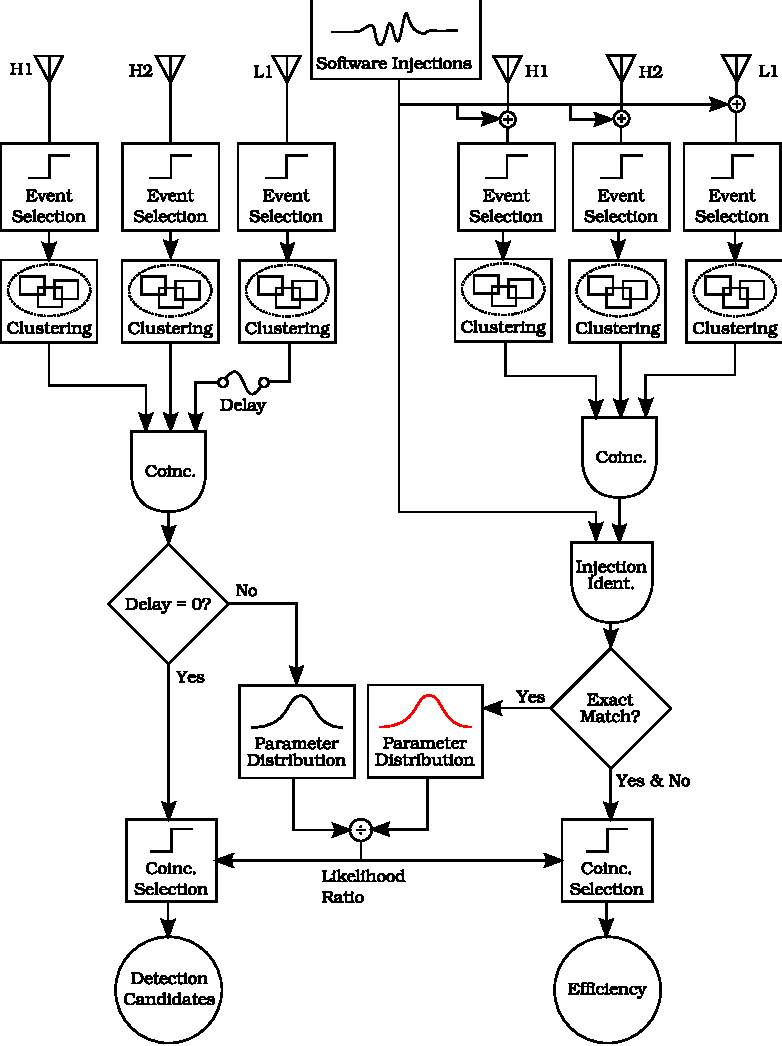
\includegraphics{figures/pipeline.pdf}\end{center}
\caption{Data flow in the excess power pipeline.}
\label{fig1}
\end{figure}
Here and in what follows we'll discuss the multi-detector version of the
pipeline.  The pipeline can analyze any number of detectors, but in the 1
detector case much of the pipeline (e.g., the coincidence stages) reduces
to no-ops and is uninteresting.

The pipeline begins by scanning the outputs of the gravitational wave
detectors for statistically significant excursions from the background
noise.  In particular, it searches for excursions from the noise, or
bursts, that can be characterized by a frequency band and time interval.
The raw events identified in the outputs of the individual detectors are
clustered, which reduces the event rate and assists in parameter
estimation.  The clusters are tested for coincidence across instruments,
that is events are discarded unless matching events are also found in all
other detectors.  A set of events that, together, passes the coincidence
test will be refered to as a coincident \(n\)-tuple.

Prior to applying the coincidence test, optional delays can be applied to
the events.  In the LIGO-only case, delays are only applied to events from
the L1 detector.  The delay facility is used to collect two populations of
coincident \(n\)-tuples:  \(n\)-tuples with delays applied which are
refered to as time-slide coincidences, and \(n\)-tuples with no delays
applied which are refered to as zero-lag coincidences.

It is also possible to insert software injections into the detector time
series.  The injection facility is used to simulate the presense of
gravitational waves in the data.  When software injections are inserted
into the time series, the coincidence test is followed by an injection
identification step.  This stage identifies two populations of recovered
injections:  injections that are recovered very well, and injections that
are recovered poorly.

The time-slide non-injection \(n\)-tuples, and the \(n\)-tuples
corresponding to well-recovered software injections are collected together
and their parameters measured to yield two distribution density functions.
The parameter distribution density function measured from the time-slide
\(n\)-tuples is interpreted as the parameter distribution for noise-like
\(n\)-tuples, while the parameter distribution density function measured
from the software injections is interpreted as the parameter distribution
for gravitational wave-like \(n\)-tuples.  The ratio of these two
distributions is used to assign a likelihood ratio to each \(n\)-tuple.

Finally, a likelihood-ratio based threshold is applied to each \(n\)-tuple.
The zero-lag \(n\)-tuples that survive this final cut are gravitational
wave detection candidates.  The same cut is applied to software injection
\(n\)-tuples to measure the detection efficiency of the pipeline.  If the
final threshold is adjusted so that just exactly 0 zero-lag \(n\)-tuples
survive, the efficiency measured for the pipeline in that configuration can
be used to derive an upper-limit result.


\section{Program \prog{lalapps\_power}}


\subsection{Man Page}


\begin{entry}

\item[Name]
\prog{lalapps\_power} --- apply excess power event selection algorithm to
real or simulated gravitational wave detector data.

\item[Synopsis]
\prog{lalapps\_power} \newline \hspace*{0.5in}
\option{--bandwidth}~\parm{Hz} \newline \hspace*{0.5in}
[\option{--burstinjection-file}~\parm{file name}] \newline \hspace*{0.5in}
[\option{--calibrated-data}] \newline \hspace*{0.5in}
[\option{--calibration-cache}~\parm{cache file}] \newline \hspace*{0.5in}
\option{--channel-name}~\parm{string} \newline \hspace*{0.5in}
\option{--confidence-threshold}~\parm{threshold} \newline \hspace*{0.5in}
[\option{--debug-level}~\option{info|warn|error|off}] \newline \hspace*{0.5in}
[\option{--dump-diagnostics~\parm{XML filename}}] \newline \hspace*{0.5in}
\option{--filter-corruption}~\parm{samples} \newline \hspace*{0.5in}
\option{--frame-cache}~\parm{cache file} \newline \hspace*{0.5in}
[\option{--gaussian-noise-rms}~\parm{RMS}] \newline \hspace*{0.5in}
\option{--gps-end-time}~\parm{seconds} \newline \hspace*{0.5in}
\option{--gps-start-time}~\parm{seconds} \newline \hspace*{0.5in}
[\option{--help}] \newline \hspace*{0.5in}
\option{--high-pass}~\parm{Hz} \newline \hspace*{0.5in}
[\option{--inspiralinjection-file}~\parm{file name}] \newline \hspace*{0.5in}
\option{--low-freq-cutoff}~\parm{Hz} \newline \hspace*{0.5in}
[\option{--max-event-rate}~\parm{Hz}] \newline \hspace*{0.5in}
\option{--max-tile-bandwidth}~\parm{Hz} \newline \hspace*{0.5in}
\option{--max-tile-duration}~\parm{seconds} \newline \hspace*{0.5in}
[\option{--mdc-cache}~\parm{cache file}] \newline \hspace*{0.5in}
[\option{--mdc-channel}~\parm{channel name}] \newline \hspace*{0.5in}
[\option{--output}~\parm{file name}] \newline \hspace*{0.5in}
\option{--psd-average-points}~\parm{samples} \newline \hspace*{0.5in}
[\option{--ram-limit}~\parm{MebiBytes}] \newline \hspace*{0.5in}
\option{--resample-rate}~\parm{Hz} \newline \hspace*{0.5in}
[\option{--sim-cache}~\parm{cache file}] \newline \hspace*{0.5in}
[\option{--sim-seconds}~\parm{sec.s}] \newline \hspace*{0.5in}
[\option{--siminjection-file}~\parm{injection file}] \newline \hspace*{0.5in}
[\option{--seed}~\parm{seed}] \newline \hspace*{0.5in}
\option{--target-sample-rate}~\parm{Hz} \newline \hspace*{0.5in}
\option{--tile-stride-fraction}~\parm{fraction} \newline \hspace*{0.5in}
[\option{--user-tag}~\parm{comment}] \newline \hspace*{0.5in}
\option{--window-length}~\parm{samples} \newline \hspace*{0.5in}

\item[Description] 
\prog{lalapps\_power} performs an excess power analysis on real or
simulated data.  This program's input consists of gravitational wave
detector time series data, and an optional list of injections to add to the
time series prior to analysis.  The program's output is a list of events
identified as being statistically significant in the input time series.

Gravitational wave detector time series data is read from LIGO/VIRGO .gwf
frame files.  This program analyzes data from only a single detector at a
time, but it can analyze data that spans multiple frame files.  Usually a
collection of frame files is specified by providing as input to this
program a LAL cache file, as might be obtained from \prog{LSCdataFind}.

If software injections are desired, then a LIGO\_LW XML file containing a
sim\_burst table describing the software injections must also be provided
as input.  In the past it has also been possible to read sim\_inspiral
tables and MDC injection frame files, but these facilities have not been
tested in a long time.  See the \prog{lalapps\_binj} program described in
Sec.~\ref{program:lalapps-binj} for information on constructing injection
description files.

The output is written to a LIGO\_LW XML file containing a sngl\_burst table
listing the events found in the input time series.  The output file also
contains process, process\_params, and search\_summary tables containing
metadata describing the analysis that was performed.  In particular, these
other tables provide precise information about the instrument and interval
of time that the program analyzed.

By default, the output file is named following the standard frame file
naming convention.
\begin{quote}
\parm{instrument}-POWER\_\parm{comment}-\parm{start}-\parm{duration}.xml
\end{quote}
For example, if a search was run on the Hanford \(\unit{4}{\kilo\metre}\)
interferometer and generated triggers starting at GPS time
\(\unit{731488397}{\second}\), the triggers cover \(\unit{33}{\second}\)
after that time, and the command line includes the option
``\option{--comment} TEST'', then the file name would be 
\begin{quote}
H1-POWER\_TEST-731488397-33.xml
\end{quote}
The output file name can be set explicitly with the \option{--output}
command line option.  If the name ends in ``.gz'', then it will be
gzip-compressed.

\item[Options]\leavevmode
\begin{entry}
\item[\option{--bandwidth} \parm{Hz}]
Set the bandwidth in which the search is to be performed.  This must be an
integer power of 2.  This and the \option{--low-freq-cutoff} option
together set the frequency band to be searched.

\item[\option{--burstinjection-file} \parm{file name}]
Read the sim\_burst table from the LIGO\_LW XML file \parm{file name}, and
add the software injections described therein to the input time series
prior to analysis.

\item[\option{--calibrated-data}]
When the \option{--calibrated-data} option is supplied, input time series
data is read as IEEE double-precision samples.  Calibrated data, for
example from the GEO detector, or from LIGO's \(h(t)\) frames, is stored in
double-precision rather than single-precision format.  The default is to
read the data as IEEE single-precision samples, although internally the
code uses double precision throughout (single-precision input data is
re-quantized to double precision prior to processing).

\item[\option{--calibration-cache} \parm{cache file}]
Specify the location of calibration information.  \parm{cache file} gives
the path to a LAL-format frame cache file describing locations of
\texttt{.gwf} frame files that provide the calibration data ($\alpha$ and
$\beta$ coefficients) for the analysis.  Frame cache files are explained in
the ``framedata'' package in LAL.

\item[\option{--channel-name} \parm{string}]
Set the name of the data channel to analyze to \parm{string}.  This must
match the name of one of the data channels in the input frame files.  For
example, ``\verb|H2:LSC-AS_Q|''.

\item[\option{--confidence-threshold} \parm{threshold}]
Set the confidence threshold below which events should be discarded.  The
``confidence'' of an event is \(-\ln P(\text{event} | \text{stationary
Gaussian white noise})\), so an event with a confidence of 30 has a
probability of \(\ee^{-30}\) of having been found in stationary Gaussian
white noise.  For the LIGO instruments, a practical treshold is typically
around 10.

\item[\option{--debug-level} \option{info|warn|error|off}]
Sets the level of verbosity:  \option{info} = print all messages,
\option{warn} = print only warnings and errors, \option{error} = print only
errors, and \option{off} = be silent.  The default value is \option{error}.

\item[\option{--dump-diagnostics \parm{XML filename}}]
Dump diagnostic snapshots of internal time and frequency series data to a
LIGO Light Weight XML file of the given name.  The file is overwritten.

\item[\option{--filter-corruption} \parm{samples}]
The input time series data is passed through a conditioning filter prior to
analysis.  Generally, the conditioning filter should be expected to corrupt
some amount of the beginning and end of the time series due to edge
effects.  This parameter tells the code how much data, in samples, should
be ignored from the start and end of the time series.  A reasonable value
is 0.5 seconds worth of data.

\item[\option{--frame-cache} \parm{cache file}]
Obtain the locations of input \texttt{.gwf} frame files from the LAL frame
cache file \parm{cache file}.  LAL frame cache files are explained in the
``framedata'' package in LAL and can be constructed by running
\prog{LSCDataFind} on some systems.  One of \option{--frame-cache}, or
\option{--gaussian-noise-rms} must be specified.

\item[\option{--gaussian-noise-rms} \parm{RMS}]
If this parameter is provided instead of \option{--frame-cache}, then
Gaussian white noise will be synthesized and used as the input data.  One
of \option{--frame-cache}, or \option{--gaussian-noise-rms} must be
specified.

\item[\option{--gps-end-time} \parm{seconds}]
Set the GPS time up to which input data should be read.  Non-integer values
are permitted, but the fractional part must not contain more than 9 digits
(accurate to nanoseconds).

\item[\option{--gps-start-time} \parm{seconds}]
Set the GPS time from which to start reading input data.  Non-integer
values are permitted, but the fractional part must not contain more than 9
digits (accurate to nanoseconds).

\item[\option{--help}]
Display a usage message and exit.

\item[\option{--high-pass} \parm{Hz}]
The input time series is high-pass filtered as part of the input data
conditioning.  This argument sets the cut-off frequency for this filter.
In older versions of the program, this frequency was hard-coded to be
\unit{10}{\hertz} below the lower bound of the frequency band being
searched or \unit{150}{Hz}, which ever was lower.

\item[\option{--inspiralinjection-file} \parm{file name}]
Use \parm{file name} as a LIGO lightweight XML file containing a list of inspiral
injections to be made.   The file should contain a \verb+sim_inspiral+ table
which is used to set information about the types of inspiral injections to be made.
This file may be constructed by hand, the
\verb+lalapps_bbhinj+ program described in the Inspiral package   

\item[\option{--low-freq-cutoff} \parm{Hz}]
Set the lower bound for the frequency band in which to search for
gravitational waves.  This and the \option{--bandwidth} option together set
the frequency band to be searched.

\item[\option{--max-event-rate} \parm{Hz}]
Exit with a failure if the event rate, averaged over the entire analysis
segment, exceeds this limit.  This provides a safety valve to prevent the
code from filling up disks if the threshold is set improperly.  A value of
0 (the default) disables this feature.

\item[\option{--max-tile-bandwidth} \parm{Hz}]
This specifies the maximum frequency bandwidth, \(B\), that a tile can
have.  This also fixes the minimum time duration of the tiles, \(\Delta t =
1/B\).  This must be an integer power of 2.

\item[\option{--max-tile-duration} \parm{s}]
This specifies the maximum duration that a tile can have.  This also fixes
the minimum bandwidth of the tiles.  This must be an integer power of 2.

\item[\option{--mdc-cache} \parm{cache file}]
Use \parm{cache file} as a LAL format frame cache file describing the
locations of MDC frames to be used for injections.

\item[\option{--mdc-channel} \parm{channel name}]
Use the data found in the channel \parm{channel name} in the MDC frames for
injections.

\item[\option{--output} \parm{file name}]
Set the name of the LIGO Light Weight XML file to which results will be
written.  The default is
``\parm{instrument}-POWER\_\parm{comment}-\parm{start}-\parm{duration}.xml''.
Where \parm{instrument} is derived from the name of the channel being
analyzed, and \parm{comment} is obtained from the command line.
\parm{start} is the integar part of the GPS start time from the command
line, and \parm{duration} is the difference of the integer parts of the
GPS start and end times from the command line.

\item[\option{--psd-average-points} \parm{samples}]
Use \parm{samples} samples from the input time series to estimate the
average power spectral density of the detector's noise.  The average PSD is
used to whiten the data prior to applying the excess power statistic.  The
number of samples used for estimating the average PSD must be commensurate
with the analysis window length and analysis window spacing --- i.e.\ an
integer number of analysis windows must fit in the data used to estimate
the average PSD --- however this program will automatically round the
actual number of samples used down to the nearest integer for which this is
true.  This elliminates the need of the user to carefully determine a valid
number for this parameter, allowing him/her to instead select a number that
matches the observed length of time for which the instrument's noise is
stationary.

\item[\option{--ram-limit} \parm{MebiBytes}]
The start and stop GPS times may encompass a greater quantity of data than
can be analyzed at once due to RAM limitations.  This parameter can be used
to tell the code how much RAM, in MebiBytes, is available on the machine,
which it then uses to heursitically guess at a maximum time series length
that should be read.  The code then loops over the input data, processing
it in chunks of this size, until it has completed the analysis.  If this
parameter is not supplied, then the entire time series for the segment
identified by the GPS start and end times will be loaded into RAM.

\item[\option{--resample-rate} \parm{Hz}]
The sample frequency to which the data should be resampled prior to
analysis.  This must be a power of 2 in the range \unit{2}{\hertz} to
\unit{16386}{\hertz} inclusively.

\item[\option{--seed} \parm{seed}]
When synthesizing Gaussian white noise with \option{--gaussian-noise-rms},
this option can be optionally used to set the random number generator's
seed.

\item[\option{--tile-stride-fraction} \parm{fraction}]
This parameter controls the amount by which adjacent time-frequency tiles
of the same size overlap one-another.  This numeric parameter must be \(=
2^{-n}\), where \(n \in \mathrm{Integers}\).  A reasonable value is 0.5,
which causes each tile to overlap its neighbours in time by \(\frac{1}{2}\)
its duration and in frequency by \(\frac{1}{2}\) its bandwidth.

\item[\option{--user-tag} \parm{comment}]
Set the user tag to the string \parm{comment}.  This string must not
contain spaces or dashes (``-'').  This string will appear in the name of
the file to which output information is written, and is recorded in the
various XML tables within the file.

\item[\option{--window-length} \parm{samples}]
Set the number of samples to use for an analysis window to \parm{samples}.
Only the central half of the window will be analyzed, the first quarter and
last quarter of the window are used as padding to avoid corruption at
certain stages of the analysis.  For example, if you wish the code to
analyze the data in 1 second windows, you need to set this parameter to the
number of samples corresponding to 2 seconds of data.  This parameter must
be a power of 2.

\end{entry}


\item[Example]
To run the program, type:
\begin{verbatim}
lalapps_power \
--bandwidth 2048 \
--calibrated-data \
--channel-name "H1:LSC-STRAIN" \
--debug-level info \
--filter-corruption 4096 \
--frame-cache H-754008315-754008371.cache \
--gps-end-time 754008363 \
--gps-start-time 754008323 \
--high-pass 60.0 \
--low-freq-cutoff 70.0 \
--max-event-rate 10000 \
--psd-average-points 274432 \
--ram-limit 1024 \
--resample-rate 8192 \
--tile-stride-fraction 0.5 \
--user-tag testing \
--window-length 16384
\end{verbatim}
For this to succeed, the current directory must contain the file
\texttt{H-754008315-754008931.cache} describing the locations of the
\texttt{.gwf} frame files containing the channel \verb|H1:LSC-STRAIN|
spanning the GPS times 754008323.0 s through 754008363.0 s.

\item[Authors]
Patrick Brady, Saikat Ray-Majumder and Kipp Cannon.  
\end{entry}


\subsection{Time-Frequency Analysis Algorithm}


\subsubsection{Overview}


The Excess Power search method is motivated by the classical theory of
signal detection in Gaussian noise.  The method is the optimal search
strategy~\cite{anderson2001}, having only knowledge of the time duration
and frequency band of the expected signal,  but having no other information
about the power distribution in advance of detection.

The algorithm amounts to projecting the data onto a basis of test
functions, each of which is a prototype for the waveforms being sought in
the data.  The projection procedure is the following.  The input time
series is passed through a comb of frequency-domain filters, generating
several output time series, one each for a number of frequency channels.
Summing the squares of the samples in any one of these channels amounts to
summing the ``energy'' in the corresponding frequency band.  Summing only
the samples from a range of times produces a number that is interpreted as
the energy in that frequency band for that period of time --- the energy in
a time-frequency tile whose bandwidth is that of the frequency channel, and
whose duration is the length of the sum.

The search is a multi-resolution search, so tiles of many different
bandwidths and durations are scanned.  For performance purposes, only a
single frequency channel decomposition is used.  ``Virtual'' wide bandwidth
channels are constructed by summing the samples from multiple channels, and
correcting for the overlap between adjacent channel filters.

Once the energy in a tile has been measured, a threshold is applied to
select the ``important'' tiles.  The quantity thresholded on is the
probability of measuring at least that much energy in a tile with that
bandwidth and that duration in stationary Gaussian noise.  The procedure
employed to assess this probability is to first whiten and normalize the
data, to transform it into what is then assumed to be stationary white
unit-variance Gaussian noise, and then read off the probability of the
observed energy from a theoretical distribution derived from that
assumption.


\subsubsection{The Whitening Procedure}


Consider a discretely-sampled time-series of \(N\) samples, \(s_j\) where
\(0 \leq j < N\) and the sample period is \(\Delta t\).  Much of the signal
processing to be described below is done in the frequency domain, so the
first step is to multiply the time series by a window function, \(w_{j}\),
tapering it to 0 at the start and end to reduce the noise arising from the
data's aperiodicity at its boundary.  The mean square of the tapering
window's samples is
\begin{equation}
\sigma_{w}^{2}
   = \frac{1}{N} \sum_{j = 0}^{N - 1} w_{j}^2.
\end{equation}
Following multiplication by the tapering window, the data is Fourier
transformed to the frequency domain.  The complex amplitude of the
frequency bin \(k\) is
\begin{equation}
\tilde{s}_{k}
   = \frac{\Delta t}{\sigma_{w}} \sum_{j = 0}^{N - 1} w_{j} s_{j} \ee^{-2
   \pi \aye j k / N},
\end{equation}
where \(0 \leq k < N\).  The frequency bins \(\lfloor N / 2 \rfloor < k <
N\) correspond to negative frequency components, and are not stored because
the input time series is real-valued and so the negative frequency
components are redundant (they are the complex conjugates of the positive
frequency components).  For the non-negative frequencies, bin \(k\)
corresponds to frequency
\begin{equation}
f_{k}
   = k \Delta f,
\end{equation}
where the bin spacing is \(\Delta f = (N \Delta t)^{-1}\).  Defining the
power spectral density as
\begin{equation}
P_{k}
   = \Delta f \mean{\magnitude{\tilde{s}_{k}}^{2} + \magnitude{\tilde{s}_{N
   - k}}^{2}}
   = 2 \Delta f \mean{\magnitude{\tilde{s}_{k}}^{2}},
\end{equation}
for \(0 \leq k < \lfloor N / 2 \rfloor\), the ``whitened'' frequency series
is
\begin{equation}
\hat{s}_{k}
   = \sqrt{\frac{2 \Delta f}{P_{k}}} \tilde{s}_{k}
\end{equation}
so that
\begin{equation}
\label{eqn3}
\mean{\magnitude{\hat{s}_{k}}^2}
   = 1.
\end{equation}
The definition of the power spectral density is such that
\begin{align}
\mean{s_{j}^{2}}
   & = \frac{1}{N^{2} \Delta t^{2}} \sum_{k = 0}^{N - 1} \sum_{k' = 0}^{N -
   1} \mean{\tilde{s}_{k} \conj{\tilde{s}}_{k'}} \ee^{2 \pi \aye j (k - k')
   / N}
   \\
   & = \frac{1}{2 N \Delta t} \sum_{k = 0}^{N - 1} P_{k},
\end{align}
when the frequency components are independent (the input time series is a
stationary process).

If the original time series is stationary Gaussian noise, this construction
makes each frequency bin's real and imaginary parts Gaussian random
variables with variances of 0.5.  The definition of the power spectral
density and of the Fourier transform shown above both match those of the
LIGO Algorithm Library, as documented in LIGO-T010095-00-Z.  Figure
\ref{fig:shistogram} shows the distribution of the real and imaginary
components of \(\hat{s}_{k}\) obtained from a sample of \(h(t)\) taken from
the LIGO L1 instrument during S4.
\begin{figure}
\begin{center}
\resizebox{5.5in}{!}{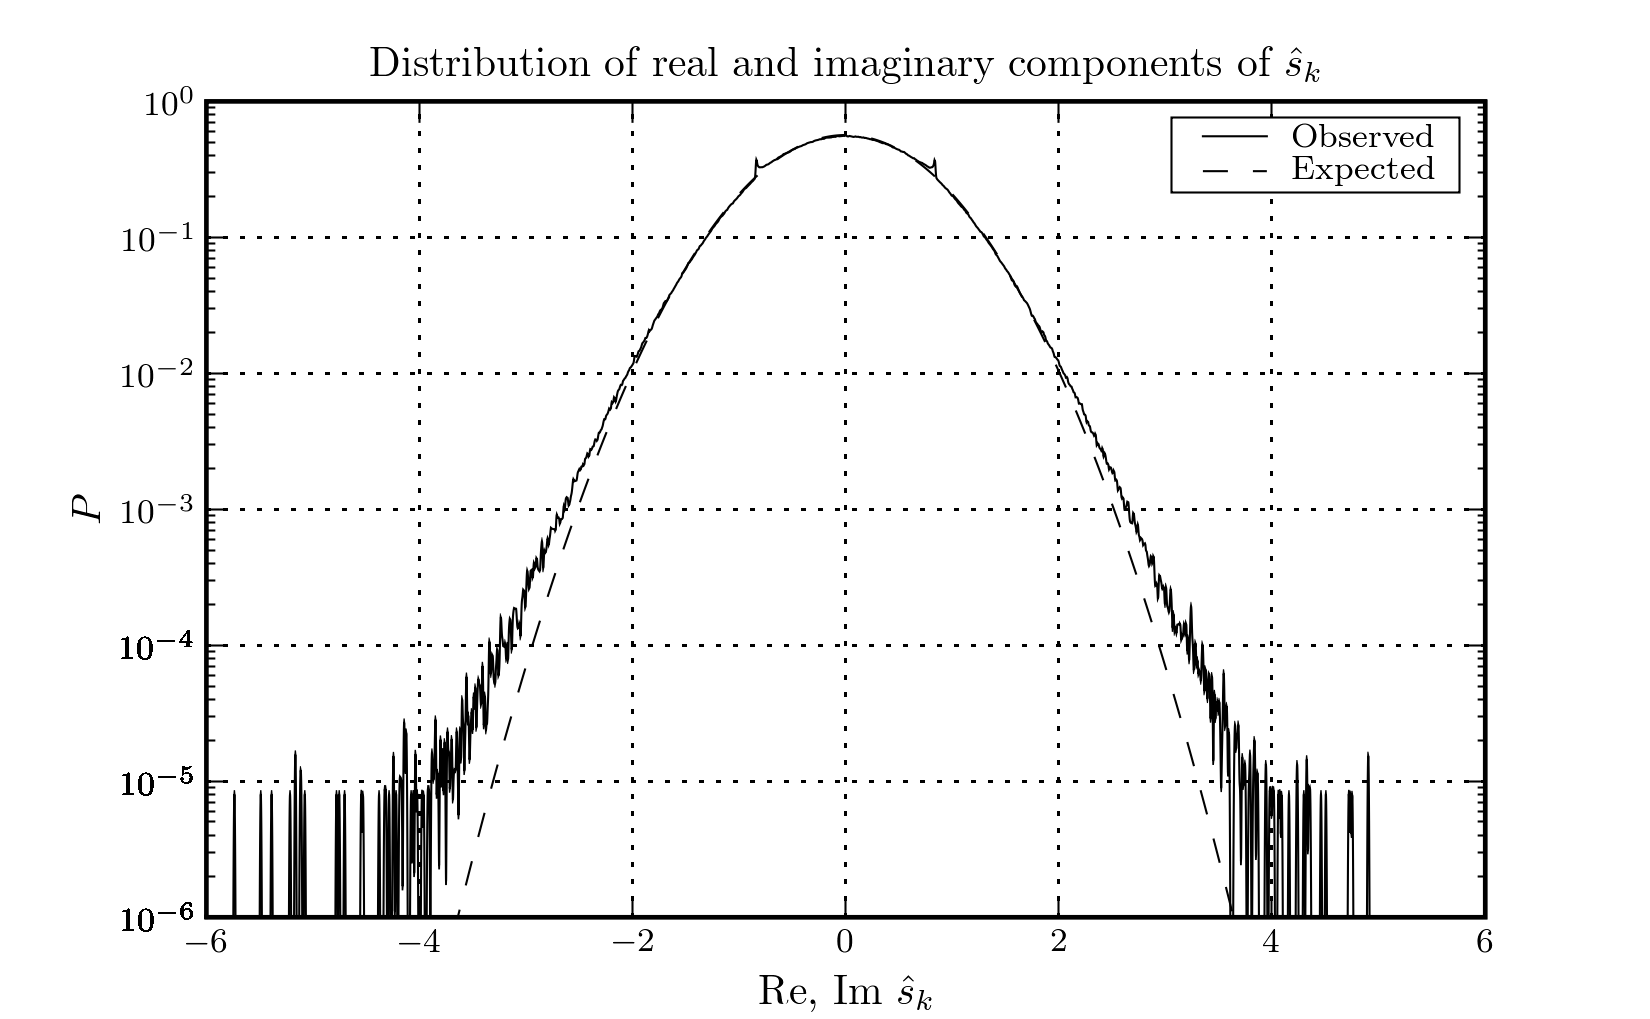
\includegraphics{figures/sk_histogram.png}}
\end{center}
\caption{The distribution of the real and imaginary components of
\(\hat{s}_{k}\) obtained from a sample of \(h(t)\) taken from the LIGO L1
instrument during S4.  The aparent bias away from the expected
normalization (actually non-Gaussianity) and the two horn features, are the
result of correlations between the power spectrum and the data.  Recall
that the power spectrum is estimated from the same data it is used to
whiten.}
\label{fig:shistogram}
\end{figure}

If the input time series is a stationary random process, then the
components of its Fourier transform are uncorrelated, and we would find
that \(\mean{\hat{s}_{k} \conj{\hat{s}}_{k'}} = \delta_{k k'}\).  However,
because we have windowed the time series (which is equivalent to convolving
its Fourier transform with that of the window), the frequency components
are now correlated.  We can compute \(\mean{\hat{s}_{k}
\conj{\hat{s}}_{k'}}\) by assuming the whitened time series consists of
independently-distributed random variables, because then the
Wiener-Khinchin theorem tells us that its two-point spectral correlation
function is the Fourier transform of its variance which we'll assume is
proportional to the square of the tapering window function.  Therefore,
\begin{equation}
\mean{\hat{s}_{k} \conj{\hat{s}}_{k'}}
   \propto \sum_{j = 0}^{N - 1} w_{j}^{2} \ee^{-2 \pi \aye j (k - k') / N}.
\end{equation}
The proportionality constant is obtained from \eqref{eqn3}, which tells us
that
\begin{equation}
\label{eqn4}
\mean{\hat{s}_{k} \conj{\hat{s}}_{k'}}
   = \frac{1}{\sigma_{w}^{2}} \sum_{j = 0}^{N - 1} w_{j}^{2} \ee^{-2 \pi
   \aye j (k - k') / N}.
\end{equation}
A comparison of this prediction to the observed two-point spectral
correlation in \(\hat{s}_{k}\) obtained from \(h(t)\) recorded at the LIGO
L1 instrument during S4 is shown in Figure \ref{fig:sksk}.
\begin{figure}
\begin{center}
\resizebox{5.5in}{!}{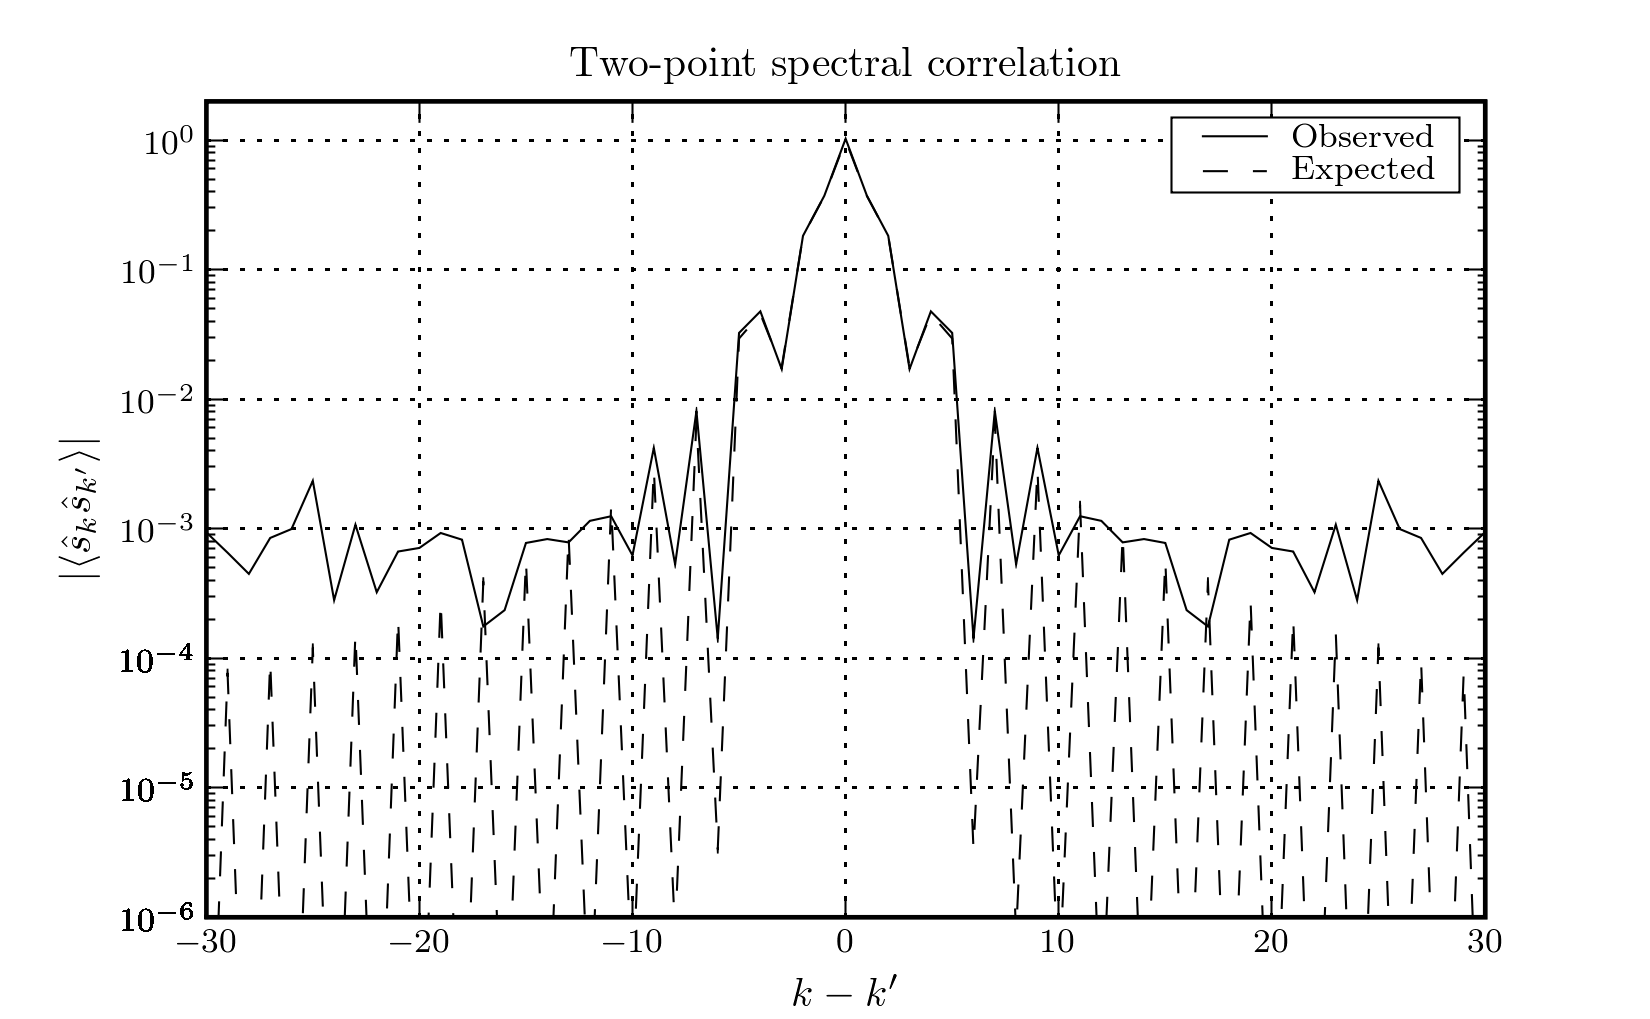
\includegraphics{figures/sksk.png}}
\end{center}
\caption{The two-point spectral correlation in the whitened data when a
Tukey window with 50\% flat top is used to taper the input time series.
The ``expected'' curve is what is expected in the limit of an average over
an infinite number of measurements.  Since a finite number of measurements
were made, a residual ``floor'' is expected, and it should go as
\((\text{number of measurements})^{-1/2}\).  Approximately 4 million
samples were averaged in each bin so the floor, which is
\(\mean{\hat{s}_{k} \conj{\hat{s}}_{k'}} \sim 2000^{-1}\), is consistent
with what is expected.}
\label{fig:sksk}
\end{figure}

The power spectral density is estimated using the median power at each
frequency for a number of overlapping segments.  The use of the median
avoids bias in the spectrum caused by the presence of a gravitational wave
or other large non-astrophysical transients present in any of the segments. 


\subsubsection{The Channel Filter}
\label{sec:channelfilter}


The choice of the channel filter is mostly irrelevant, except that it
correspond in some meaningful way to a particular frequency band.  We'll
denote the channel filter spanning frequencyes \(f_{1} \leq f_{k} < f_{2}\)
as \(\tilde{\Theta}_{k}(f_{1}, B)\), where the bandwidth of the filter is
\(B = f_{2} - f_{1}\).  If \(b\) is the bandwidth of the narrowest channel,
excess power achieves a multi-resolution search by computing only the
narrowest channels, and choosing
\begin{equation}
\tilde{\Theta}_{k}(f_{1}, n b)
   = \sum_{i = 0}^{n - 1} \Theta_{k}(f_{1} + i b, b),
\end{equation}
where \(B = n b\).  That is, the filters for wide band channels are chosen
to be the sums of adjacent filters from narrower bands.  The specific
choice made in excess power is to use Hann windows for the narrowest
channels.  The narrow channels are all the same width, and the Hann windows
are adjusted to be centred on their channel and extend over a range of
frequencies twice the width of the channel,
\begin{equation}
\tilde{\Theta}_{k}(f_{1}, b)
   \propto \begin{cases}
   \sin^{2} \frac{\pi}{2 b} (f_{k} - f_{1} + \frac{b}{2}), & f_{1} -
   \frac{b}{2} \leq f_{k} < f_{1} + \frac{3 b}{2} \\
   0, & \text{othewise}.
   \end{cases}
\end{equation}
In this way, when the filters for two adjacent channels are summed the
result is a Tukey window --- a window with a flat top in the middle and
\(\sin^{2}\) tapers at each end.

All windows are real-valued, so that they are phase preserving.  The
narrowest channel filters, the filters of bandwidth \(b\),  are normalized
so that
\begin{equation}
\label{eqn5}
\sum_{k = 0}^{N - 1} \sum_{k' = 0}^{N - 1} -1^{(k - k')} \mean{\hat{s}_{k}
\conj{\hat{s}}_{k'}} \conj{\tilde{\Theta}}_{k}(f_{1}, b)
\tilde{\Theta}_{k'}(f_{1}, b)
   = \frac{b}{\Delta f},
\end{equation}
where the two-point spectral correlation is given in \eqref{eqn4}.  The
reason for this choice will become clear later.  For convenience, let us
introduce the notation
\begin{equation}
\left\{ \tilde{X}, \tilde{Y} \right\}
   = \sum_{k = 0}^{N - 1} \sum_{k' = 0}^{N - 1} -1^{(k - k')}
   \mean{\hat{s}_{k} \conj{\hat{s}}_{k'}} \conj{\tilde{X}}_{k}
   \tilde{Y}_{k'},
\end{equation}
so
\begin{equation}
\left\{ \tilde{\Theta}(f_{1}, b), \tilde{\Theta}(f_{1}, b) \right\}
   = \frac{b}{\Delta f}.
\end{equation}
Notice that if the two-point spectral correlation is a Kroniker \(\delta\)
(the input data is not windowed), and the channel filter is flat,
\(\tilde{\Theta}_{k} = \tilde{\Theta}\), and spans the entire frequency
band from DC to Nyquist, \(b / \Delta f = N\), then the normalization would
lead to
\begin{equation}
\tilde{\Theta}
   = 1.
\end{equation}

In the LIGO Algorithm Library, the Fourier transforms of real-valued time
series contain only postive frequency components (the negative frequency
components being the complex conjugates of these), and so the channel
filters are also stored as only positive frequency components.  Since the
two-point spectral correlation function is usually strongly-peaked around
\(k - k' = 0\), and since the channel filters all go to zero far from the
DC and Nyquist components, in practice it is safe to sum over only the
positive frequency components, and require the sum to be
\begin{equation}
2 \sum_{k = 0}^{\lfloor N / 2 \rfloor + 1} \sum_{k' = 0}^{\lfloor N / 2
\rfloor + 1} -1^{(k - k')} \mean{\hat{s}_{k} \conj{\hat{s}}_{k'}}
\conj{\tilde{\Theta}}_{k}(f_{1}, b) \tilde{\Theta}_{k'}(f_{1}, b)
   = \frac{b}{\Delta f}.
\end{equation}
So the argument is that in practice this normalization is identical to
\eqref{eqn5}, but it is easier to implement because these are the only
components stored in memory.

For wide channels, channels formed by summing the filters from two or more
narrow channels, the ``magnitude'' of the channel filter will not be \(n b
/ \Delta f\).  For example,
\begin{equation}
\tilde{\Theta}_{k}(f_{1}, 2 b)
   = \tilde{\Theta}_{k}(f_{1}, b) + \tilde{\Theta}_{k}(f_{1} + b, b),
\end{equation}
and using the symmetry of \(\mean{\hat{s}_{k} \conj{\hat{s}}_{k'}}\) the
magnitude of this channel filter is found to be
\begin{align}
\left\{ \tilde{\Theta}(f_{1}, 2 b), \tilde{\Theta}(f_{1}, 2 b) \right\}
   & = \frac{2 b}{\Delta f} + 2 \left\{ \tilde{\Theta}(f_{1}, b),
   \tilde{\Theta}(f_{1} + b, b) \right\}.
\end{align}
The channel construction described above, with Hann windows for the
narrowest channels yielding Tukey windows for wider channels, allows us to
make the approximation that only adjacent channel filters have sufficient
overlap that their inner products are non-zero, and so the cross terms from
adjacent channels are the only ones that need to be accounted for.
Therefore, in general, a filter spanning \(n\) channels is
\begin{equation}
\tilde{\Theta}_{k}(f_{1}, n b)
   = \sum_{i = 0}^{n - 1} \tilde{\Theta}_{k}(f_{1} + i b, b),
\end{equation}
and its magnitude is
\begin{equation}
\left\{ \tilde{\Theta}(f_{1}, n b), \tilde{\Theta}(f_{1}, n b) \right\}
   = \frac{n b}{\Delta f} + 2 \sum_{i = 0}^{n - 2} \left\{
   \tilde{\Theta}(f_{1} + i b, b), \tilde{\Theta}(f_{1} + (i + 1) b, b)
   \right\}.
\end{equation}
Let us denote this magnitude as \(\mu^{2}(f_{1}, n b)\),
\begin{equation}
\label{eqn2}
\mu^{2}(f_{1}, n b)
   = \frac{n b}{\Delta f} + 2 \sum_{i = 0}^{n - 2} \sum_{k = 0}^{N - 1}
   \sum_{k' = 0}^{N - 1} -1^{(k - k')} \mean{\hat{s}_{k}
   \conj{\hat{s}}_{k'}} \tilde{\Theta}_{k}(f_{1} + i b, b)
   \conj{\tilde{\Theta}}_{k'}(f_{1} + (i + 1) b, b).
\end{equation}
When \(n = 1\), \(\mu^{2} = b / \Delta f\).

Figure \ref{fig:freqdomainfilter} illustrates the construction of a
\(\unit{16}{\hertz}\) channel filter from four \(\unit{4}{\hertz}\) channel
filters when \(\mean{\hat{s}_{k} \conj{\hat{s}}_{k'}} = \delta_{k k'}\).
\begin{figure}
\begin{center}
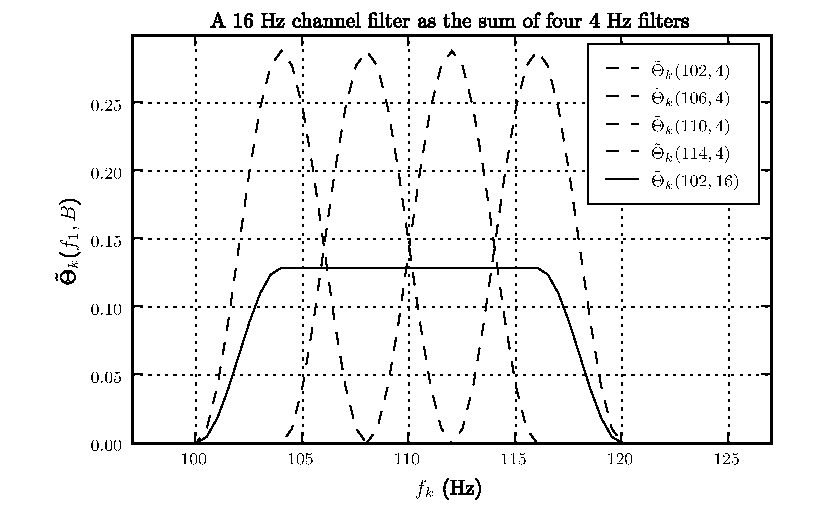
\includegraphics{figures/freqdomainfilter.pdf}
\end{center}
\caption{Summing narrow Hann channel filters to obtain wide-band Tukey
filters.}
\label{fig:freqdomainfilter}
\end{figure}
The \(\unit{16}{\hertz}\) channel filter has had its normalization adjusted
by the factor in \eqref{eqn2} to illustrate the relative amplitudes of the
channel filters when all are normalized to have magnitudes of 1.  This
figure also shows how the approximation that only adjacent channels have
non-zero overlap becomes exact in the limit of a two-point spectral
correlation function that is a Kroniker \(\delta\) (the ``tapering'' window
is flat, \(w_{j} = 1\)), because the third channel filter can only overlap
the first when there is mixing between \(k\).  The time-domain versions of
two sample channel filters are shown in Figure \ref{fig:timedomainfilter}.
\begin{figure}
\begin{center}
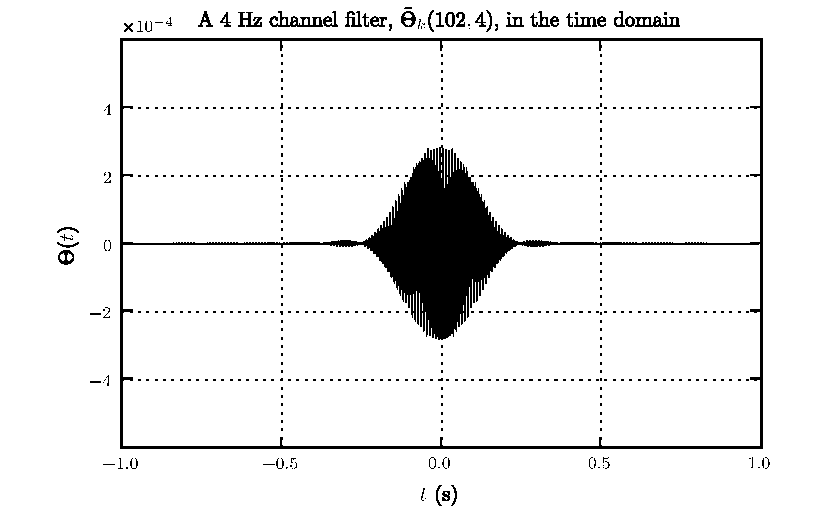
\includegraphics{figures/timedomainfilter_04hz.pdf}
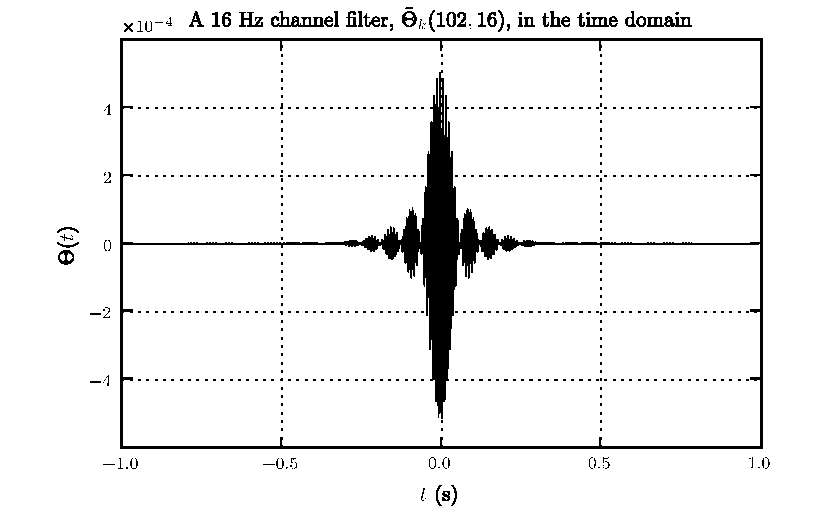
\includegraphics{figures/timedomainfilter_16hz.pdf}
\end{center}
\caption{Two examples of channel filters in the time domain.}
\label{fig:timedomainfilter}
\end{figure}


\subsubsection{The Channel Time Series}


The time series for a channel is extracted by multiplying the whitened
frequency-domain input data by the channel filter, and transforming the
result back to the time domain.  The time series for the channel of
bandwidth \(b\) starting at frequency \(f_{1}\) is
\begin{equation}
\label{eqn1}
z_{j}(f_{1}, b)
   = \frac{1}{N \Delta t} \sum_{k = 0}^{N - 1} \hat{s}_{k}
   \conj{\tilde{\Theta}}_{k}(f_{1}, b) \ee^{2 \pi \aye j k / N},
\end{equation}
and the mean square is
\begin{equation}
\mean{z_{j}^{2}(f_{1}, b)}
   = \frac{1}{N^{2} \Delta t^{2}} \sum_{k = 0}^{N - 1} \sum_{k' = 0}^{N -
   1} \mean{\hat{s}_{k} \conj{\hat{s}}_{k'}}
   \conj{\tilde{\Theta}}_{k}(f_{1}, b) \tilde{\Theta}_{k'}(f_{1}, b) \ee^{2
   \pi \aye j (k - k') / N}.
\end{equation}
The mean square is sample-dependent (depends on \(j\)) because the original
time series had the window \(w_{j}\) applied to it.  We will now require
that the window be of a kind with a flat portion in the middle, so that
\begin{equation}
w_{j}
   = \begin{cases}
   1 & \text{if \(0 \leq j_{1} \leq j < j_{2} \leq N\)},
   \\
   \leq 1 & \text{otherwise}.
   \end{cases}
\end{equation}
For example, a Tukey window is suitable.  In that case, the mean square of
\(z_{j}(f_{1}, b)\) should be independent of \(j\) when \(j_{1} \leq j <
j_{2}\).  If we further require the flat portion of the window to be in the
middle, in other words require \(j_{1}\) and \(j_{2}\) to be such that
\(j_{1} \leq N / 2 < j_{2}\), then we can pick \(j = N / 2\) as
representative of the mean square of \(z_{j}(f_{1}, b)\) in the flat
portion of the window.  Therefore,
\begin{equation}
\mean{z_{j}^{2}(f_{1}, b)}
   = \frac{1}{N^{2} \Delta t^{2}} \sum_{k = 0}^{N - 1} \sum_{k' = 0}^{N -
   1} -1^{(k - k')} \mean{\hat{s}_{k} \conj{\hat{s}}_{k'}}
   \conj{\tilde{\Theta}}_{k}(f_{1}, b) \tilde{\Theta}_{k'}(f_{1}, b).
\end{equation}
From the normalization of the channel filters (the motivation for the
formulation of which is now seen), the sum is \(b / \Delta f\), and
therefore
\begin{equation}
\mean{z_{j}^{2}(f_{1}, b)}
   = \frac{1}{N^{2} \Delta t^{2}} \frac{b}{\Delta f},
\end{equation}
for \(j_{1} \leq j < j_{2}\).

The LIGO Algorithm Library's \texttt{XLALREAL4ReverseFFT()} function
computes the inverse transform omitting the factor of \(\Delta f = 1 / (N
\Delta t)\) that appears in \eqref{eqn1}.  The time series returned by this
function is
\begin{equation}
Z_{j}(f_{1}, b)
   = N \Delta t z_{j}(f_{1}, b),
\end{equation}
and the mean squares of the samples in the time series are
\begin{equation}
\mean{Z_{j}^{2}(f_{1}, b)}
   = \frac{b}{\Delta f},
\end{equation}
for \(j_{1} \leq j < j_{2}\).  For a channel spanning \(n\) narrow
channels,
\begin{align}
Z_{j}(f_{1}, n b)
   & = \sum_{k = 0}^{N - 1} \hat{s}_{k} \conj{\tilde{\Theta}}_{k}(f_{1}, n
   b) \ee^{2 \pi \aye j k / N}
   \\
   & = \sum_{k = 0}^{N - 1} \hat{s}_{k} \left( \sum_{i = 0}^{n - 1}
   \conj{\tilde{\Theta}}_{k}(f_{1} + i b, b) \right) \ee^{2 \pi \aye j k /
   N}
   \\
   & = \sum_{i = 0}^{n - 1} Z_{j}(f_{1} + i b, b),
\end{align}
and so the samples in the time series for a wide channel are obtained by
summing the samples from the appropriate narrow channel time series.  The
mean squares of the samples of a wide channel's time series are given by
the quantity in \eqref{eqn2},
\begin{equation}
\mean{Z_{j}^{2}(f_{1}, n b)}
   = \mu^{2}(f_{1}, n b).
\end{equation}

Figure \ref{fig:Zhistogram} shows the distribution of \(Z_{j}(f_{1}, B)\)
observed in the same data used to measure the \(\hat{s}_{k}\) distribution
in Figure \ref{fig:shistogram}.
\begin{figure}
\begin{center}
\resizebox{5.5in}{!}{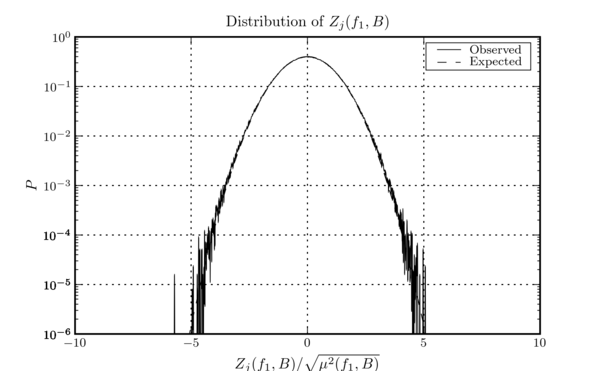
\includegraphics{figures/Z_histogram.png}}
\end{center}
\caption{The distribution of \(Z_{j}(f_{1}, B) / \sqrt{\mu^{2}(f_{1}, B)}\)
observed in data derived from a sample of \(h(t)\) taken from the LIGO L1
instrument during S4.  This distribution is measured from all samples used
to form time-frequency tiles.}
\label{fig:Zhistogram}
\end{figure}
This distribution appears more Gaussian than does the distribution of the
real and imaginary components of the whitened frequency series, and
generally exhibits better agreement with its expected behaviour.
Presumably this is a result of the central limit theorem:  the real and
imaginary components of the whitened frequency series may not be Gaussian,
but they do have unit variance, and since the time-domain samples of
\(Z_{j}\) are computed from many thousands of frequency bins, they end up
being unit variance Gaussian random variables.


\subsubsection{The Time-Frequency Tile}


Having projected the whitened input time series onto a comb of frequency
channels, including channels with a variety of widths, we now procede to
project it onto a collection of time-frequency tiles.  For this, we need to
know that the number of degrees of freedom in a tile of bandwidth \(B\) and
duration \(T\) is
\begin{equation}
d
   = 2 B T.
\end{equation}
This can be understood as follows.  A real-valued signal with a bandwidth
of \(B\) can be represented without loss of information as a discrete
real-valued time series with a sample rate equal to the Nyquist frequency
\(2 B\) (the time series may be a heterodyned version of the signal).
Therefore, \(2 B T\) real-valued samples are sufficient to encode all the
information contained in a signal of bandwidth \(B\) and duration \(T\).
We will require the number of degrees of freedom to be an even integer not
less than 2.

To construct the time-frequency tile spanning the frequencies \(f_{1} \leq
f < f_{1} + B\), and the times \(t_{1} \leq t < t_{1} + T\), we will use
the samples from the channel time series \(Z_{j}(f_{1}, B)\).  The channel
time series' sample period is \(\Delta t\), the same sample period as the
original input time series, but because the channel time series corresponds
to a more narrow frequency band than does the original input time series
(except in the special case of a channel spanning the entire input band),
there are more samples per unit time in the channel time series than there
are degrees of freedom per unit time --- the channel time series is over
sampled.  To obtain a time series with the correct sample rate, a sample
rate matching the actual number of degrees of freedom per second, we need
to down-sample the channel time series.

Let \(j_{1} = t_{1} / \Delta t\) be the time series sample index
corresponding to the start time of the tile.  The tile's duration spans a
total of \(T / \Delta t\) samples in the channel time series, but the tile
has \(d\) degrees of freedom so we need to down-sample the channel time
series so that from the \(T / \Delta t\) samples starting at \(j_{1}\) we
are left with \(d\) linearly independent numbers.  A simple down sampling
procedure is to select \(d\) evenly-spaced samples from the \(T / \Delta
t\) samples starting at \(j_{1}\).  Let these be the \(d\) samples at the
indices
\begin{equation}
\label{eqn8}
j
   = j_{1} + (i + \frac{1}{2}) \Delta j,
\end{equation}
where \(i = 0, \ldots, d - 1\), and \(\Delta j = T / (d \Delta t)\).  These
samples are linearly independent in the sense that it is not possible to
compute any one of them from the \(d - 1\) other samples, but they are
correlated because of the impulse response of the channel filter in the
time domain.  See, for example, Figure \ref{fig:timedomainfilter}.  In what
follows we will need the \(d\) samples forming the time-frequency tile to
be independent Gaussian random variables when the input time series is
stationary Gaussian noise.

Let us say that our \(d\) samples are the result of convolving the channel
impulse response with the ``real'' samples, and assume that if we
deconvolve the channel's impulse response from our samples we will be left
with \(d\) independent random variables.  The impulse response is
proportional to the inverse Fourier transform of the channel filter,
\begin{equation}
\Theta_{j}(f_{1}, B)
   = \frac{1}{N \Delta t} \sum_{k = 0}^{N - 1} \tilde{\Theta}_{k}(f_{1}, B)
   \ee^{2 \pi \aye j k / N}.
\end{equation}
Labeling the ``real'' samples as \(Z_{j}'(f_{1}, B)\), our assumption is
that our samples are derived from them by
\begin{equation}
\begin{bmatrix}
\vdots \\
Z_{j}(f_{1}, B) \\
\vdots
\end{bmatrix}
   \propto \begin{bmatrix}
   & \vdots & \\
   \cdots & \Theta_{j - j'}(f_{1}, B) & \cdots \\
   & \vdots &
   \end{bmatrix}
   \begin{bmatrix}
   \vdots \\
   Z_{j'}'(f_{1}, B) \\
   \vdots
   \end{bmatrix},
\end{equation}
where the \(j\) and \(j'\) indices are taken from \eqref{eqn8}.  Let's
write this matrix equation as
\begin{equation}
\vec{Z}(f_{1}, B)
   \propto \bar{\Theta}(f_{1}, B) \cdot \vec{Z}'(f_{1}, B).
\end{equation}
Inverting the equation gives the ``real'' samples in terms of our measured
samples,
\begin{equation}
\vec{Z}'(f_{1}, B)
   \propto \bar{\Theta}^{-1}(f_{1}, B) \cdot \vec{Z}(f_{1}, B).
\end{equation}
The proportionality constant is obtained by demanding that
\(\mean{Z_{j'}'^{2}(f_{1}, B)} = 1\).


\subsubsection{Excess Power (Energy)}


We define the whitened energy contained in the tile spanning the
frequencies \(f_{1} \leq f < f_{1} + B\) and the times \(t_{1} \leq t <
t_{1} + T\) as the sum of the squares of the down-sampled channel time
series
\begin{align}
E
   & = \frac{1}{\mu^{2}(f_{1}, B)} \vec{Z}(f_{1}, B) \cdot \vec{Z}(f_{1},
   B)
   \\
\label{eqn6}
   & = \frac{1}{\mu^{2}(f_{1}, B)} \sum_{i = 0}^{d - 1} Z_{j_{1} + (i +
   \frac{1}{2}) \Delta j}^{2}(f_{1}, B),
\end{align}
where \(j_{1} = t_{1} / \Delta t\) is the time series index corresponding
to the start of the tile, and \(\Delta j = T / (d \Delta t)\) is the number
of time series samples separating pixels in the time-frequency tile.

When the input time series is stationary Gaussian noise, \(E\) is the sum
of the squares of \(d\) Gaussian random variables each of whose mean is 0
and whose mean square is 1 (the factor of \(\mu^{2}\) normalizes them).
Therefore, \(E\) should be a \(\chi^{2}\)-distributed random variable of
\(d\) degrees of freedom.  Having measured an \(E\) for a tile, we can
calculate the probability that a tile would be found with at least that
\(E\) in stationary Gaussian noise, and threshold on this probability.  We
discard all tiles except those for which this probability is close to 0.
The tiling results in a large number of tiles being tested in every second
of data, and so a practical threshold is \(P(\geq E) \sim 10^{-7}\),
yielding an event rate of \(\unit{\order(\text{few})}{\hertz}\).  Figure
\ref{fig:ehistogram} shows a histogram of whitened tile energies observed
in the same strain data used to generate Figures \ref{fig:shistogram} and
\ref{fig:Zhistogram}.
\begin{figure}
\begin{center}
\resizebox{5.5in}{!}{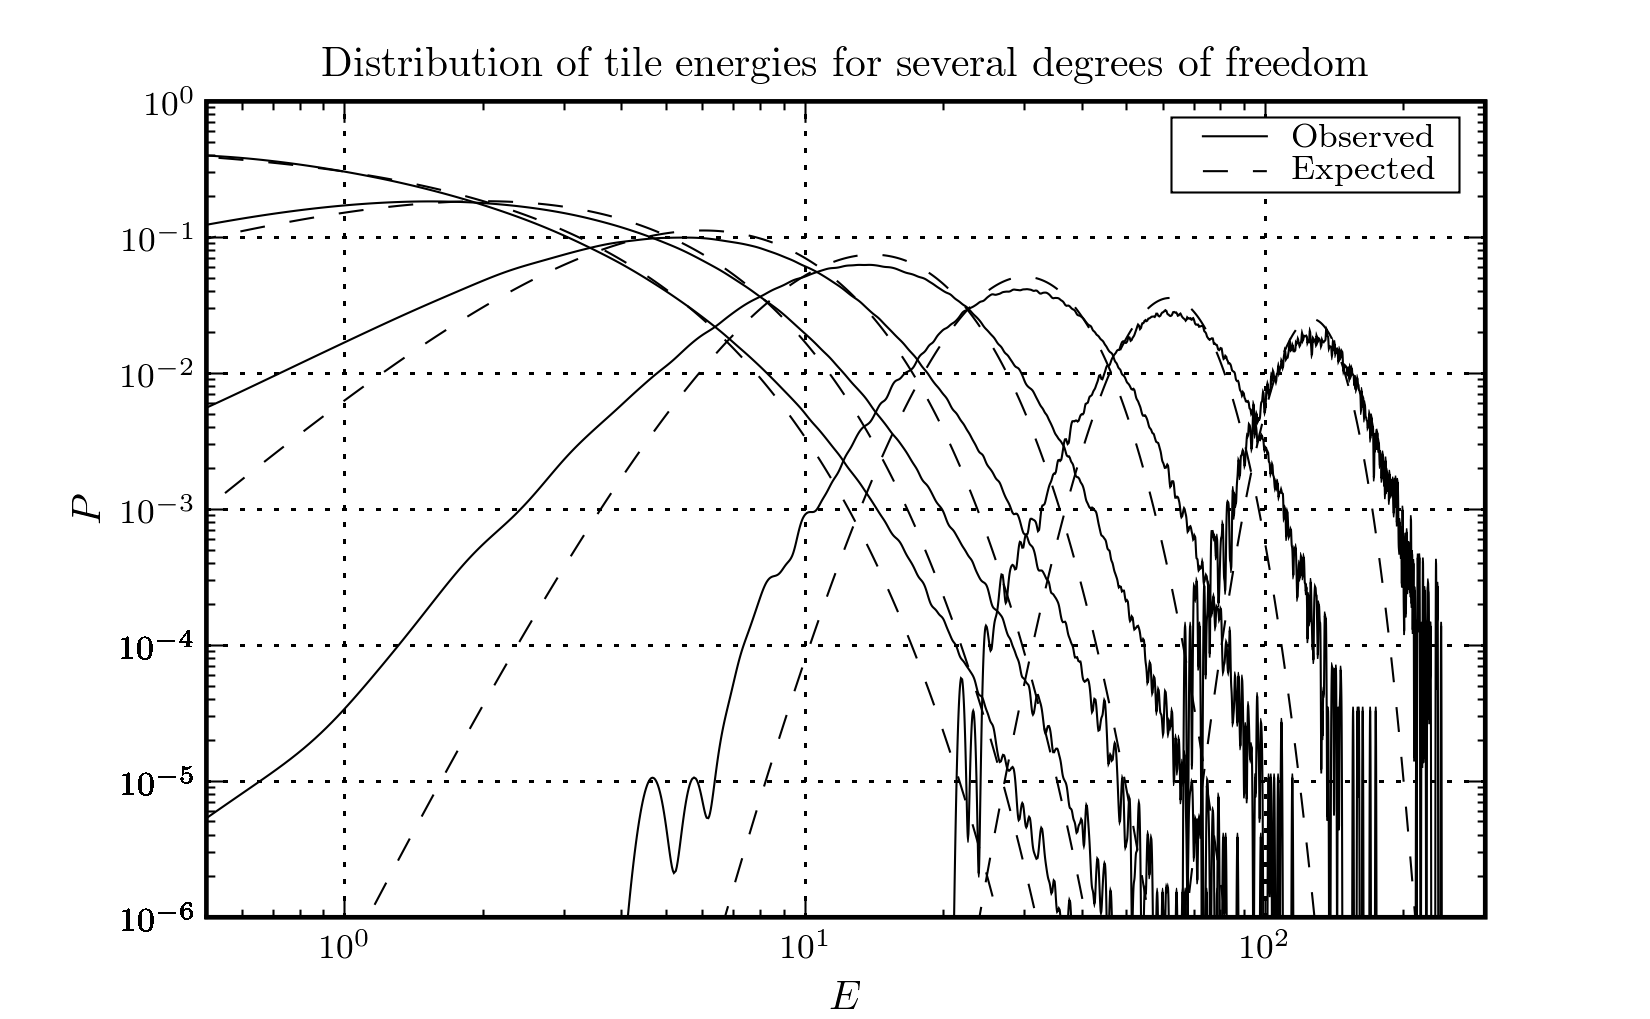
\includegraphics{figures/tiles_histogram.png}}
\resizebox{3.5in}{!}{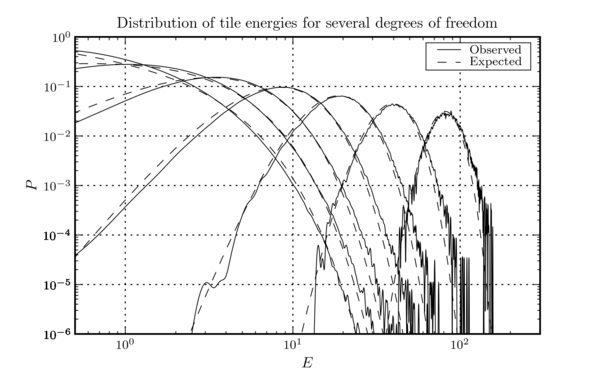
\includegraphics{figures/tiles_histogram_adjusted.png}}
\end{center}
\caption{The distribution of tile energies observed in a sample of \(h(t)\)
data collected from LIGO's L1 instrument during S4, the same data used to
obtain Figure \ref{fig:Zhistogram}.  The curves, in left-to-right order,
correspond to tiles with \(d = 2\), 4, 8, 16, 32, 64, and 128 degrees of
freedom.  The means appear to agree well with the expected values, but the
variances are little higher than expected.  This is consistent with the
tiles possessing fewer degrees of freedom than believed, which is
demonstrated in the smaller image where the energies and number of degrees
of freedom have been multiplied by 0.65, and the agreement has improved.
This is likely the result of the overlap of the channel responses in the
time domain.}
\label{fig:ehistogram}
\end{figure}

When a tile is identified as being unusual, the event is recorded in the
output file, and several properties of the event are measured and recorded.
One property is the ``confidence'', defined as
\begin{equation}
\text{confidence}
   = -\ln P(\geq E),
\end{equation}
the negative of the natural logarithm of the probability of observing a
tile with a whitened energy of \(E\) or greater in stationary Gaussian
noise.  This probability is typically close to 0, so the natural logarithm
is a large negative number, and the confidence a large positive number.
Larger ``confidence'' means a tile less like one would find in stationary
Gaussian noise.  A second quantity recorded for each event is the
signal-to-noise ratio (SNR).  The ``excess power'' (really excess energy),
of an event is
\begin{equation}
\text{excess power}
   = E - d.
\end{equation}
The expectation value of the whitened energy is \(\mean{E} = d\), so \(E -
d\) is the amount of whitened energy in the time-frequency tile beyond what
was expected --- the ``signal''.  Since the expected whitened energy is
\(d\), the SNR is
\begin{equation}
\rho
   = \frac{E - d}{d}.
\end{equation}


\subsubsection{Estimating \(h_{\text{rss}}\)}


The final quantity recorded for each event is the root-sum-squared strain,
or \(h_{\text{rss}}\).  We want the \(h_{\text{rss}}\) associated with a
particular time-frequency tile, and to do this we would like to have the
strain time series for the channel from which the time-frequency tile has
been constructed, \(h_{j}(f_{1}, B)\).  Unfortunately, we don't have this
information because we don't know what of the data is noise and what is
gravitational wave strain.  However, if we assume that the strain time
series and the noise time series are independent of one another, then the
mean square of data time series is the sum of the mean squares of the
strain and gravitational wave time series,
\begin{equation}
\mean{s_{j}^{2}(f_{1}, B)}
   = \mean{h_{j}^{2}(f_{1}, B)} + \mean{n_{j}^{2}(f_{1}, B)}.
\end{equation}
This is true on average, but we can use it to estimate the sum-of-squares
of \(h\) by summing the squares of \(s\) and subtracing the estimate of the
sum-of-squares of \(n\) derived from the measured power spectral density.
Essentially, we measure the ``energy'' in a time-frequency tile, and
subtract the mean noise energy to leave us with the gravitational wave
strain energy.  Therefore,
\begin{align}
\sum_{d} h_{j}^{2}(f_{1}, B)
   & = \left( \sum_{d} s_{j}^{2}(f_{1}, B) \right) - d
   \mean{n_{j}^{2}(f_{1}, B)}
   \\
   & = \left( \sum_{d} s_{j}^{2}(f_{1}, B) \right) - d
   \mean{s_{j}^{2}(f_{1}, B)}.
\end{align}
In this last line the notation has gotten a little confusing.  There is the
actual sum of squares of the data, and there is the expected sum of
squares.  We are using the (measured) mean square of the data in place of
the mean square of the noise on the assumption that it is noise that
dominates this quantity.  Also, \(\sum_{d}\) indicates the sum of \(d\)
time samples whose indices are the same as was used in \eqref{eqn6}.

The unwhitened time series corresponding to a single frequency channel is
the inverse Fourier transform of the unwhitened frequency series input data
multiplied by the corresponding channel filter,
\begin{align}
s_{j}(f_{1}, b)
   & = \frac{1}{N \Delta t} \sum_{k = 0}^{N - 1} \tilde{s}_{k}
   \conj{\tilde{\Theta}}_{k}(f_{1}, b) \ee^{2 \pi \aye j k / N}
   \\
   & = \frac{1}{N \Delta t \sqrt{2 \Delta f}} \sum_{k = 0}^{N - 1}
   \sqrt{P_{k}} \hat{s}_{k} \conj{\tilde{\Theta}}_{k}(f_{1}, b) \ee^{2 \pi
   \aye j k / N}
   \\
\label{eqn7}
   & = \frac{1}{\sqrt{2 N \Delta t}} \sum_{k = 0}^{N - 1} \sqrt{P_{k}}
   \hat{s}_{k} \conj{\tilde{\Theta}}_{k}(f_{1}, b) \ee^{2 \pi \aye j k /
   N}.
\end{align}
For a wide channel, \(\tilde{\Theta}_{k}(f_{1}, n b)\), we find just as for
\(Z_{j}(f_{1}, n b)\), that
\begin{equation}
s_{j}(f_{1}, n b)
   = \sum_{i = 0}^{n - 1} s_{j}(f_{1} + i b, b).
\end{equation}
The mean square of the unwhitened time series for a single channel is
\begin{equation}
\mean{s_{j}^{2}(f_{1}, b)}
   = \frac{1}{2 N \Delta t} \sum_{k = 0}^{N - 1} \sum_{k' = 0}^{N - 1}
   \sqrt{P_{k} P_{k'}} \mean{\hat{s}_{k} \conj{\hat{s}}_{k'}}
   \conj{\tilde{\Theta}}_{k}(f_{1}, b) \tilde{\Theta}_{k'}(f_{1}, b)
   \ee^{2 \pi \aye j (k - k') / N}.
\end{equation}
Making the same assumption as before, that the time series' mean square is
independent of the sample index \(j\) in the flat part of the input
tapering window, we can set \(j = N / 2\) inside the sum to leave us with
\begin{equation}
\mean{s_{j}^{2}(f_{1}, b)}
   = \frac{1}{2 N \Delta t} \sum_{k = 0}^{N - 1} \sum_{k' = 0}^{N - 1}
   -1^{(k - k')} \sqrt{P_{k} P_{k'}} \mean{\hat{s}_{k} \conj{\hat{s}}_{k'}}
   \conj{\tilde{\Theta}}_{k}(f_{1}, b) \tilde{\Theta}_{k'}(f_{1}, b).
\end{equation}
The double sum is a spectral density weighted version of the inner product
defined earlier for channel filters.  Introducing the notation
\begin{equation}
\left\{ X, Y; P \right\}
   = \sum_{k = 0}^{N - 1} \sum_{k' = 0}^{N - 1} -1^{(k - k')} \sqrt{P_{k}
   P_{k'}} \mean{\hat{s}_{k} \conj{\hat{s}}_{k'}} \conj{X}_{k} Y_{k},
\end{equation}
we can write the mean square as
\begin{equation}
\mean{s_{j}^{2}(f_{1}, b)}
   = \frac{1}{2 N \Delta t} \left\{ \tilde{\Theta}(f_{1}, b),
   \tilde{\Theta}(f_{1}, b); P \right\}.
\end{equation}
If we again make the assumption that only adjacent channels have any
significant non-zero overlap, then the mean square of the samples in an
unwhitened wide channel is
\begin{equation}
\mean{s_{j}^{2}(f_{1}, n b)}
   = \sum_{i = 0}^{n - 1} \mean{s_{j}^{2}(f_{1} + i b, b)} + \frac{1}{N
   \Delta t} \sum_{i = 0}^{n - 2} \left\{ \tilde{\Theta}(f_{1} + i b, b),
   \tilde{\Theta}(f_{1} + (i + 1) b, b) ; P \right\}.
\end{equation}

We need the \(s_{j}(f_{1}, n b)\) time series in order to compute the
unwhitened sum-of-squares for a particular tile, but constructing this time
series explicitly with the likes of \eqref{eqn7} incurs a factor of 2 cost
in both time and memory.  An approximation that works well in practice is
to assume that single channels of bandwidth \(b\) are sufficiently narrow
that the power spectral density is approximately constant in each one.
This allows \(P_{k}\) in \eqref{eqn7} to be replaced with some sort of
average and factored out of the sum to leave
\begin{equation}
s_{j}(f_{1}, b)
   \propto Z_{j}(f_{1}, b).
\end{equation}
The constant of proportionality is obtained from the known mean squares of
\(s_{j}(f_{1}, b)\) and \(Z_{j}(f_{1}, b)\), both of which are computed
(almost) without approximation.  Therefore,
\begin{equation}
s_{j}(f_{1}, b)
   \approx \sqrt{\frac{\Delta f}{b}} \sqrt{\mean{s_{j}^{2}(f_{1}, b)}}
   Z_{j}(f_{1}, b).
\end{equation}
We compute \(s_{j}(f_{1}, n b)\) for a wide channel by summing samples
across narrow channels,
\begin{equation}
s_{j}(f_{1}, n b)
   = \sum_{i = 0}^{n -1} s_{j}(f_{1} + i b, b) \propto \sqrt{\frac{\Delta
   f}{b}} \sum_{i = 0}^{n -1} \sqrt{\mean{s_{j}^{2}(f_{1} + i b, b)}}
   Z_{j}(f_{1} + i b, b),
\end{equation}
and again we solve for the proportionality constant from the ratio of the
mean squares of the left- and right-hand sides.  The mean square of the
left-hand side is given above, and that of the right-hand side is
\begin{multline}
\mean{\left( \sqrt{\frac{\Delta f}{b}} \sum_{i = 0}^{n -1}
\sqrt{\mean{s_{j}^{2}(f_{1} + i b, b)}} Z_{j}(f_{1} + i b, b) \right)^{2}}
   = \sum_{i = 0}^{n -1} \mean{s_{j}^{2}(f_{1} + i b, b)} \\+ \frac{2
   \Delta f}{b} \sum_{i = 0}^{n - 2} \sqrt{\mean{s_{j}^{2}(f_{1} + i b, b)}
   \mean{s_{j}^{2}(f_{1} + (i + 1) b, b)}} \left\{ \tilde{\Theta}(f_{1} + i
   b, b), \tilde{\Theta}(f_{1} + (i + 1) b, b) \right\}.
\end{multline}
Denoting the ratio as
\begin{equation}
\Upsilon^{2}(f_{1}, n b)
   = \mean{s_{j}^{2}(f_{1}, n b)} \mean{\left( \sum_{i = 0}^{n -1}
   \sqrt{\mean{s_{j}^{2}(f_{1} + i b, b)}} Z_{j}(f_{1} + i b, b)
   \right)^{2}}^{-1},
\end{equation}
the approximate unwhitened time series is
\begin{equation}
s_{j}(f_{1}, n b)
   \approx \sqrt{\Upsilon^{2}(f_{1}, n b)} \sqrt{\frac{\Delta f}{b}}
   \sum_{i = 0}^{n -1} \sqrt{\mean{s_{j}^{2}(f_{1}, b)}} Z_{j}(f_{1}, b).
\end{equation}
Figure \ref{fig:sjhistogram} shows a comparison of the distribution
observed in the samples of the approximate unwhitened time series
\(s_{j}(f_{1}, n b)\) values, for all bandwidths, as derived from the same
sample of \(h(t)\) recorded at the LIGO Livingston L1 instrument during S4
that has been used for the other plots.
\begin{figure}
\begin{center}
\resizebox{5.5in}{!}{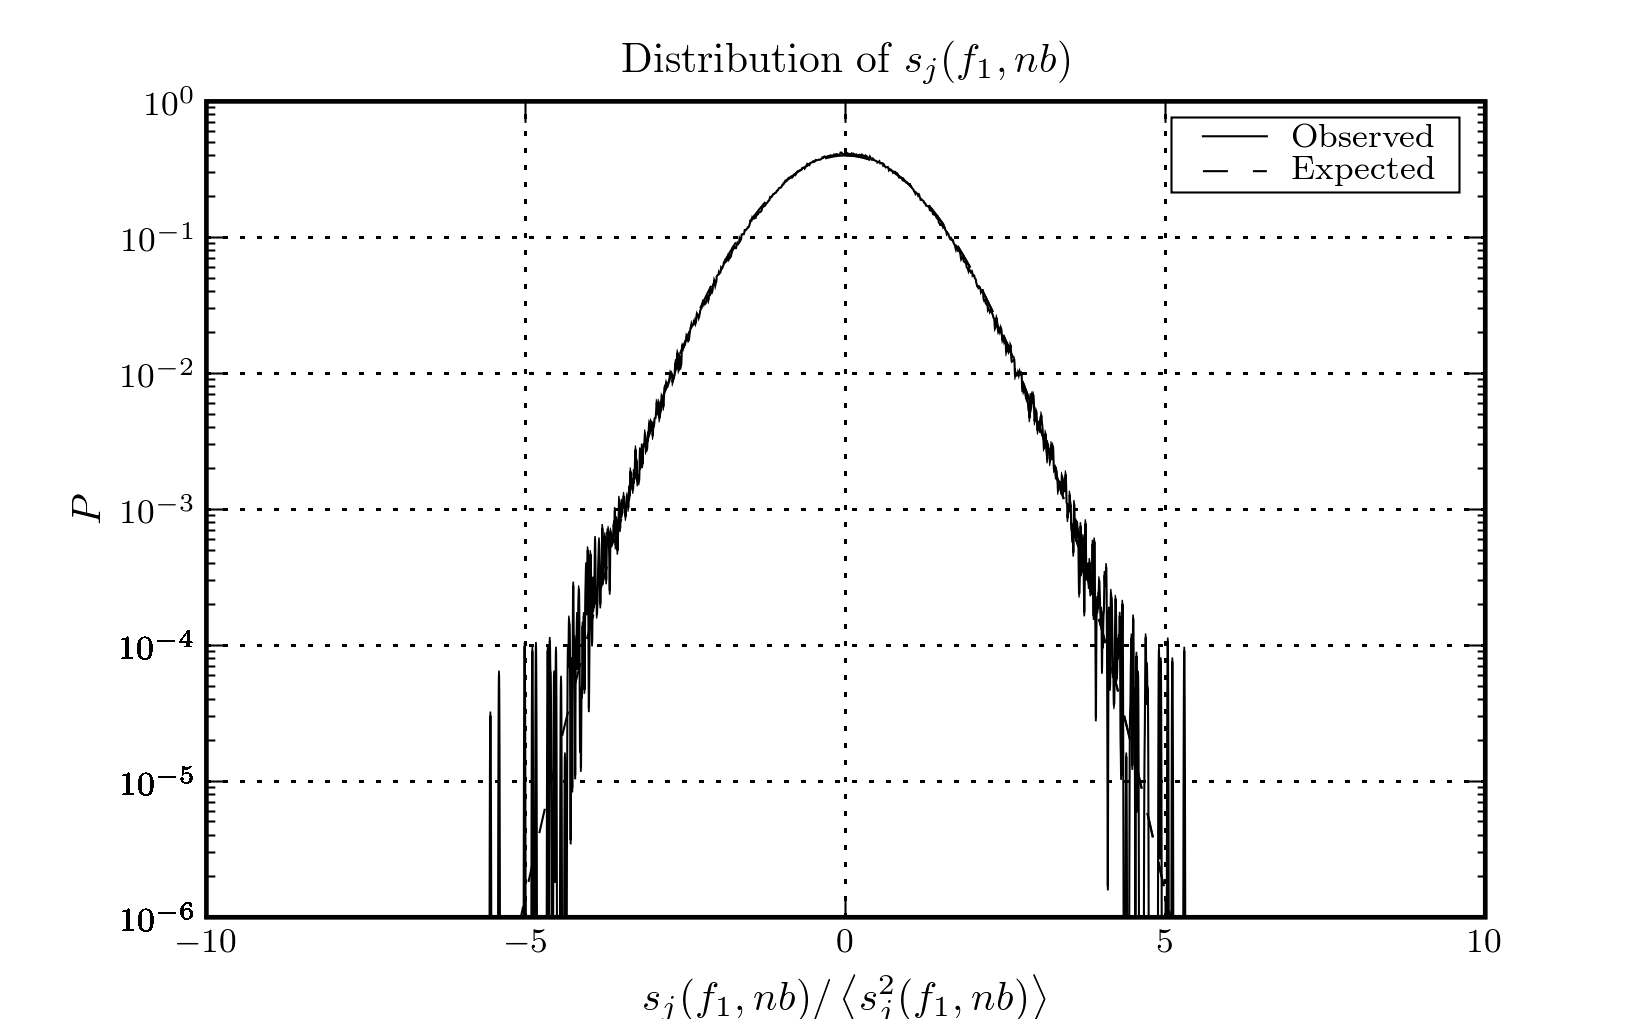
\includegraphics{figures/h_histogram.png}}
\end{center}
\caption{The distribution of samples observed in the approximate unwhitened
time series (of varying bandwidths) normalized to the expected root mean
square value.}
\label{fig:sjhistogram}
\end{figure}

Finally,
\begin{equation}
\sum_{j} h_{j}^{2}(f_{1}, n b) \Delta t
   = \sum_{j} s_{j}^{2}(f_{1}, n b) \Delta t - d \mean{s_{j}^{2}(f_{1}, n
   b)} \Delta t,
\end{equation}
so,
\begin{equation}
h_{\text{rss}}
   = \sqrt{\sum_{j} s_{j}^{2}(f_{1}, n b) \Delta t - d
   \mean{s_{j}^{2}(f_{1}, n b)} \Delta t}.
\end{equation}
A example of the results can be see in Figures \ref{fig:h_rec_vs_inj}.
\begin{figure}
\begin{center}
\resizebox{3.75in}{!}{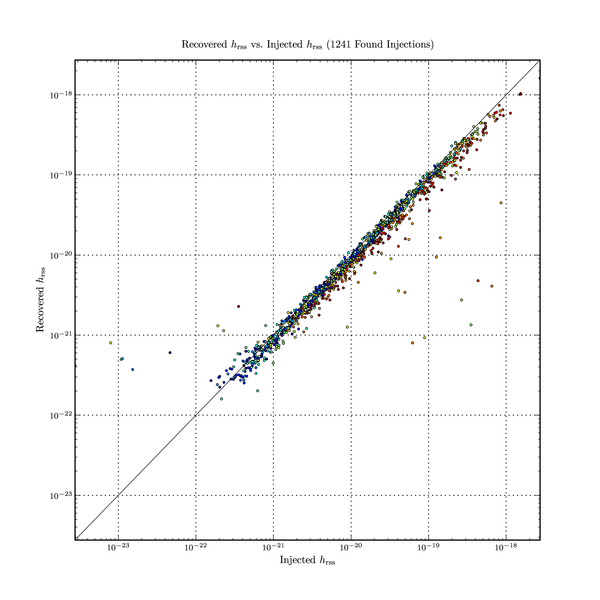
\includegraphics{figures/plotbinj_L1_4.png}}
\resizebox{3.75in}{!}{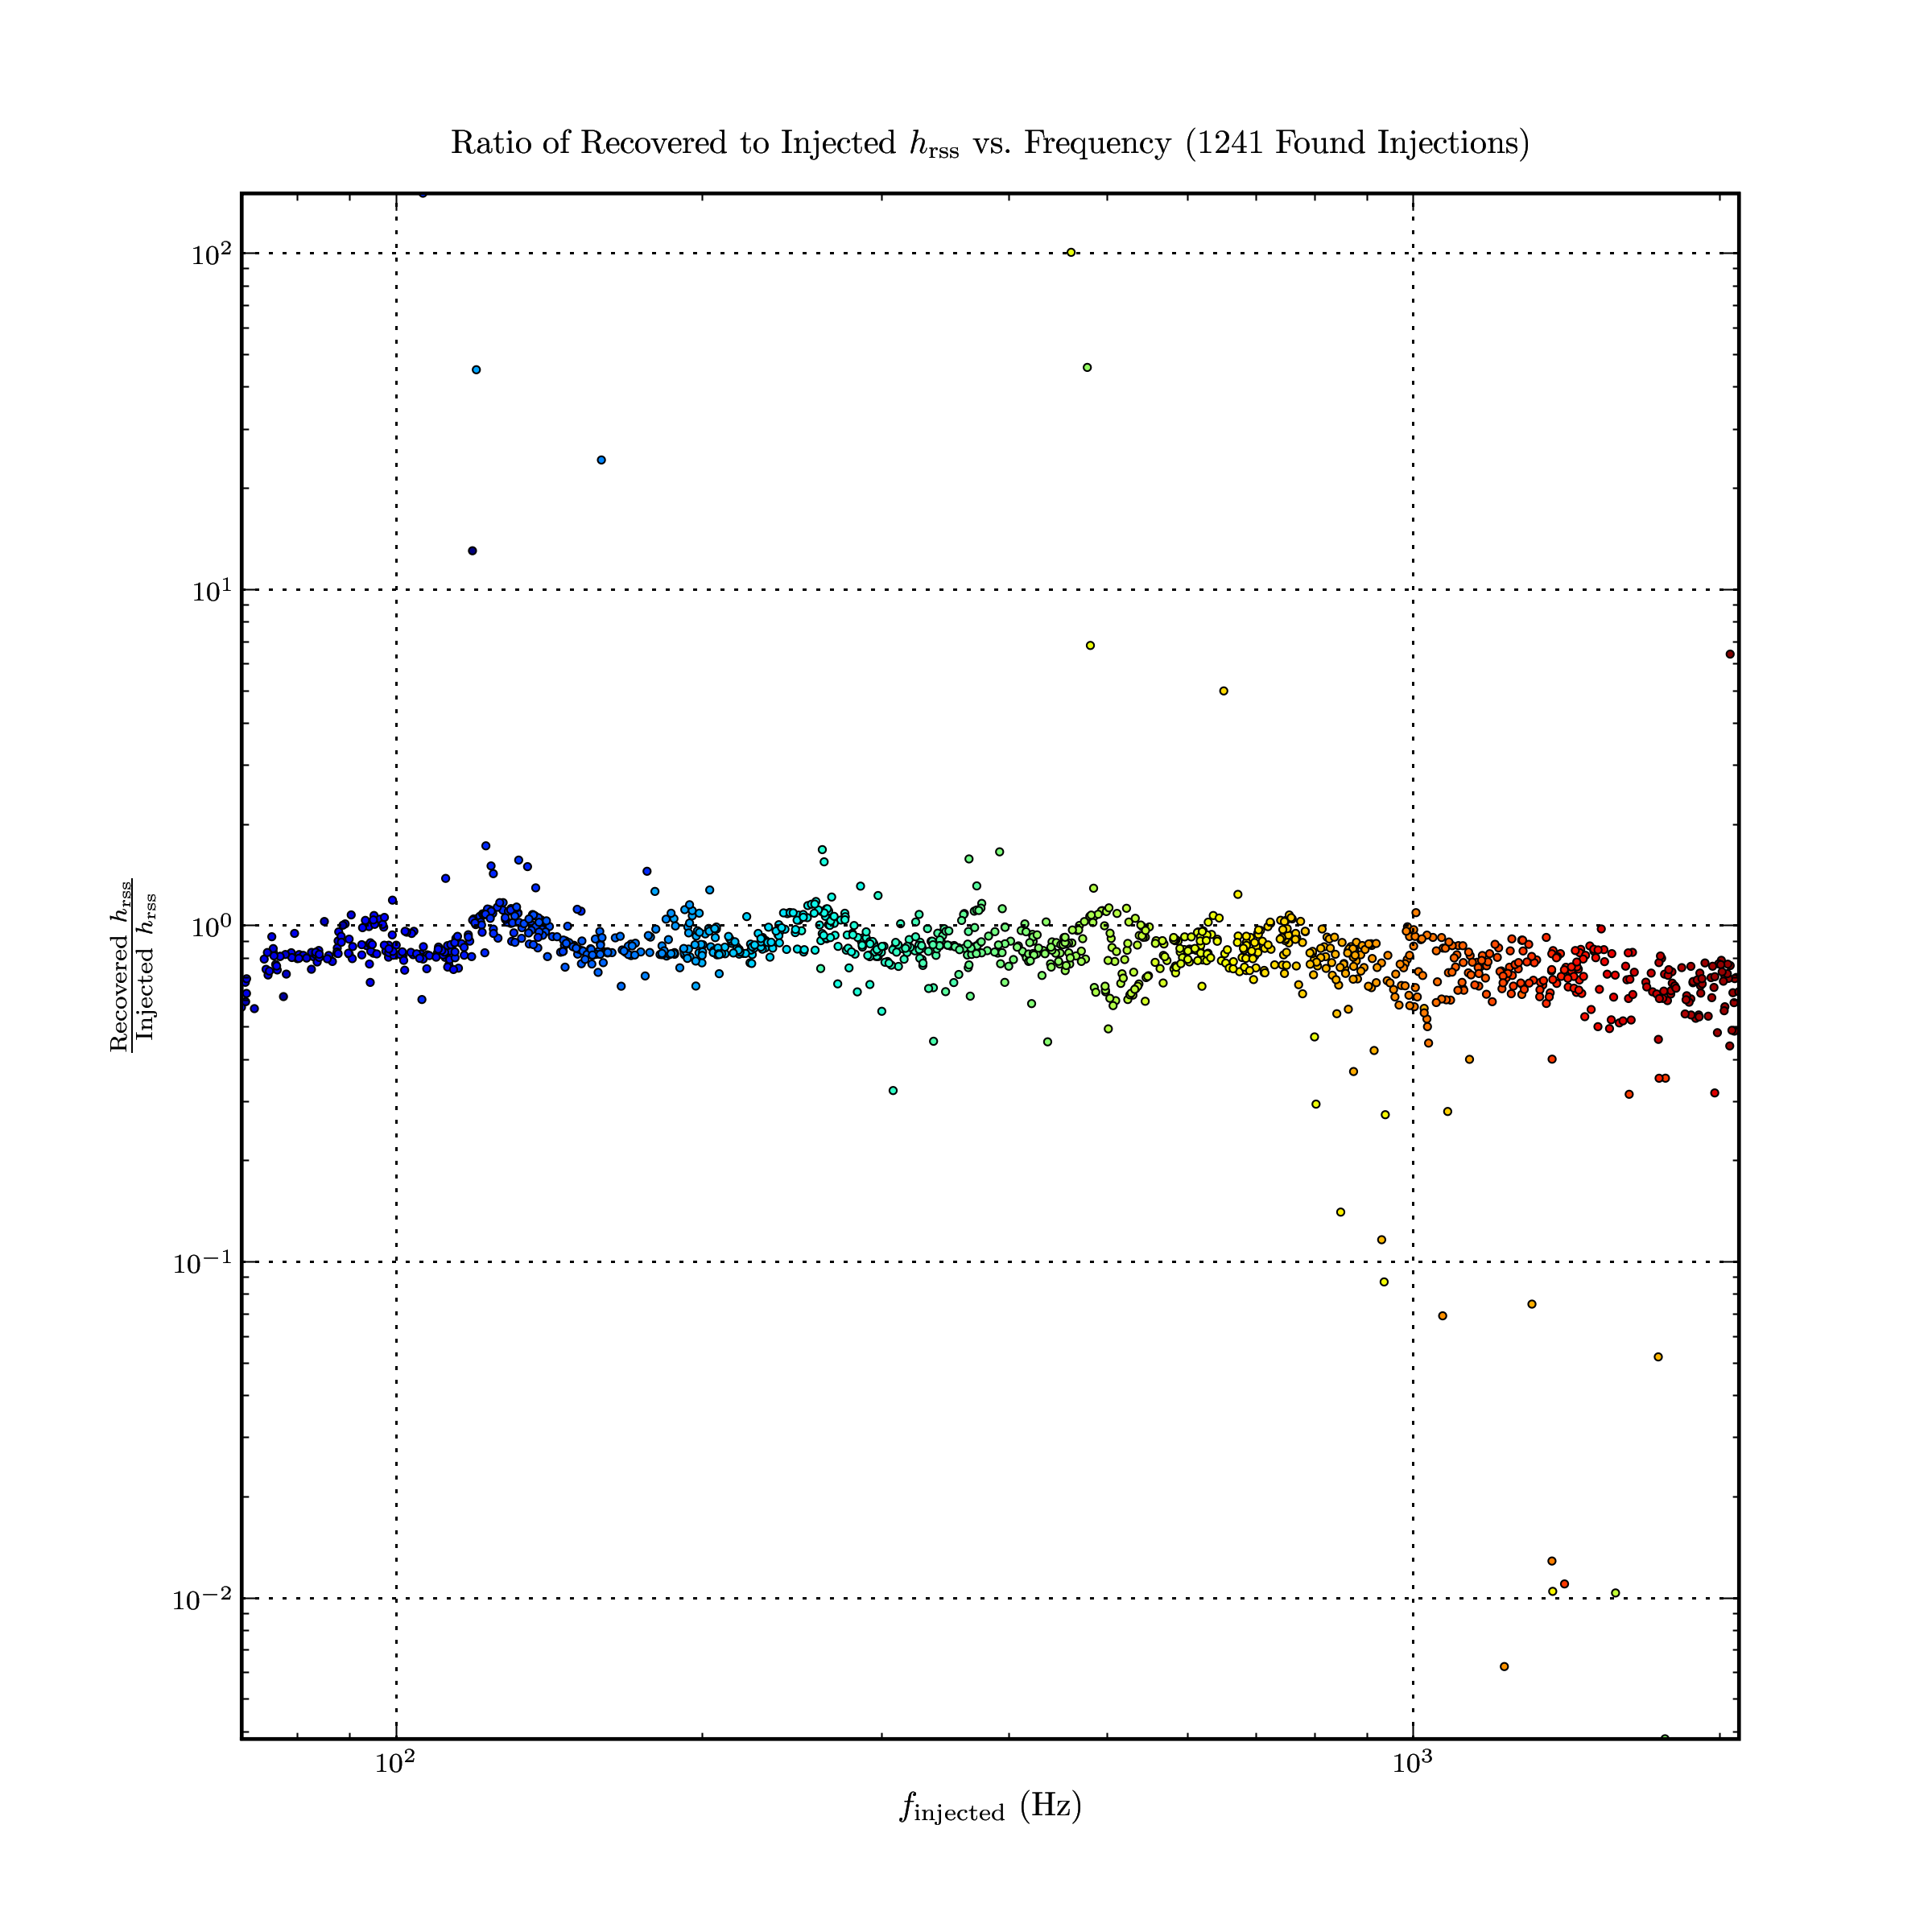
\includegraphics{figures/plotbinj_L1_5.png}}
\end{center}
\caption{Scatter plots of recovered vs.\ injected
\(h_{\text{rss}}^{\text{det}}\) for an all-sky population of \(Q = 8.89\)
sine-Gaussian linearly-polarized waveforms.  In both plots colour indicates
the frequency at which the event was recovered.  The top plot is recovered
vs.\ injected \(h_{\text{rss}}^{\text{det}}\), the bottom plot shows the
recovered-to-injected ratio vs.\ frequency at which the event was
injected.}
\label{fig:h_rec_vs_inj}
\end{figure}

It must be remarked that this procedure can occasionally yield an estimated
\(h_{\text{rss}}\) that is not real-valued.  This happens when the observed
unwhitened energy, \(\sum_{j} s_{j}^{2} \Delta t\), proves to be less than
the expected unwhitened energy, \(d \mean{s_{j}^{2}} \Delta t\).  The
whitened energy is always greater than the expected amount by construction
because we threshold on it, discarding any tiles below some cut-off.
Another way of expressing this is to say that the whitened SNR is always
greater than 1, but the unwhitened SNR need not be.  This should not be
unexpected because the arithmetic by which the frequency-domain data is
turned into a whitened and unwhitened sum-squares weights different
frequency bins differently.  In particular, non-real \(h_{\text{rss}}\)
values are seen more frequency in the vicinity of strong line features such
as the violin modes, where the difference between the whitened and
unwhitened spectra are the greatest.  The search code discards any tiles
whose estimated \(h_{\text{rss}}\) is not real-valued.


\subsubsection{Over-Whitening}


Section \ref{sec:channelfilter} began with the comment that the choice of
channel filter is mostly irrelevant, so long as there is some sense in
which it corresponds to a particular frequency band.  In the derivations
that followed, the approximation was made that only adjacent channel
filters have any appreciable overlap.  A particular choice of channel
filter was described, but other choices are possible.  One improvement that
can be made is to identify lines in the spectral density, and add notches
to the channel filters to remove them.  Often these spectral line features
are the result of noise processes in the instrument or its environment.
For example, suspension wire resonances, harmonics of the
\(\unit{60}{\hertz}\) power line frequency, and optic resonances are all
prominently visible in the spectrum of LIGO interfermeter.  The effect of
adding notches at these frequencies is to cause the search to measure the
energy in the time-frequency tiles preferentially from those frequency
bands less contaminated by these noise sources.

A simple way of deweighting contaminated frequency bands is to divide the
channel filters by some power of the power spectral density,
\begin{equation}
\tilde{\Theta}_{k}'(f_{1}, B)
   \propto P_{k}^{-a} \tilde{\Theta}_{k}(f_{1}, B).
\end{equation}
The modified channel filters are normalized as before.  When \(a =
\frac{1}{2}\), that is the nominal channel filters are divided by the
square root of the power spectral density, the procedure is called ``over
whitening''.  There are, aparently, theoretical reasons to make this
choice.  Over-whitening is found to significantly improve the ability of
the excess power search to reject noise, and so the actual channel filters
used by the search are not only the Hann windows described above but also
contain one inverse power of the square root of the power spectral density.


\subsection{Time Domain Segmentation}


%
% FIXME:  the descriptions here are obsolete
%


The excess power analysis code does not process the input data as a
continuous time series;  rather the time series is split into a sequence of
discrete ``analysis windows'', which are each analyzed individually.  To
account for the possibility of a burst event stradling the boundary between
two analysis windows, successive windows are staggered in such a way that
they overlap one another in time.  In this way, a burst event occuring on
the boundary of one window will (typically) be centred in the next.

Because edge effects at various stages of the analysis can corrupt the
beginning and end of the analysis window, the actual quantity of data
extracted from the input time series to form a window is twice the amount
that is analyzed.  Only results from the central half of the window are
retained, with the first and last quarters of each window being discarded.
The arrangement is shown in the following diagram.
\begin{center}
\begin{picture}(0,0)%
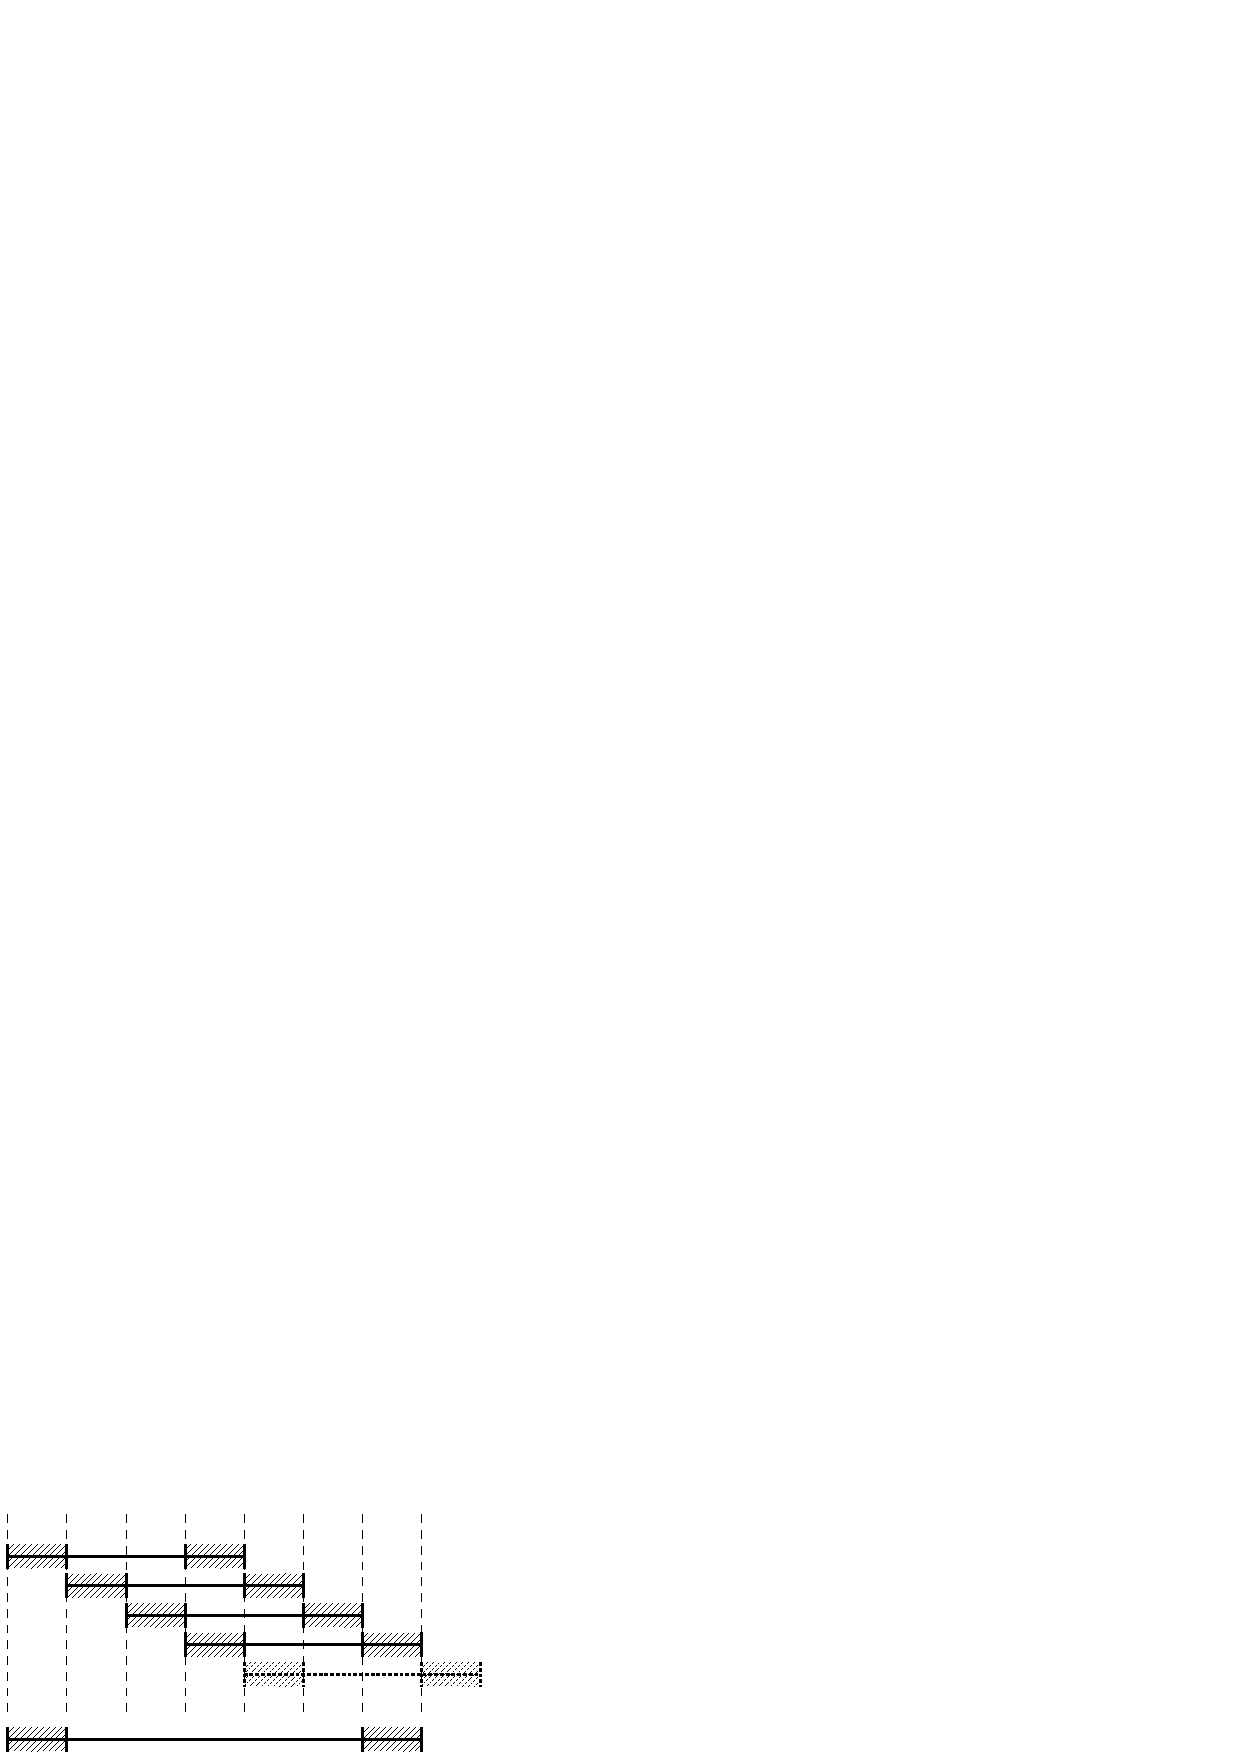
\includegraphics{figures/power/windows.fig.pdf}%
\end{picture}%
\setlength{\unitlength}{4144sp}%
%
\begingroup\makeatletter\ifx\SetFigFont\undefined%
\gdef\SetFigFont#1#2#3#4#5{%
  \reset@font\fontsize{#1}{#2pt}%
  \fontfamily{#3}\fontseries{#4}\fontshape{#5}%
  \selectfont}%
\fi\endgroup%
\begin{picture}(3194,1329)(-21,-253)
\put( 46,929){\makebox(0,0)[lb]{\smash{{\SetFigFont{10}{12.0}{\familydefault}{\mddefault}{\updefault}0}}}}
\put(1846,929){\makebox(0,0)[lb]{\smash{{\SetFigFont{10}{12.0}{\familydefault}{\mddefault}{\updefault}32768}}}}
\put(3151,434){\makebox(0,0)[lb]{\smash{{\SetFigFont{10}{12.0}{\familydefault}{\mddefault}{\updefault}\(\cdots\)}}}}
\end{picture}%

\end{center}
Here we see a discrete time series (represented by the bottom-most
horizontal line) that contains 57344 samples.  It has been divided into a
sequence of four analysis windows, each containing 32768 samples.  A fifth,
greyed-out, analysis window is shown to indicate where the next window in
the sequence would start.  In the analysis of each window, the first and
last 8192 samples (first and last quarter) are discarded as indicated by
the crossed-out sections in each window.  In this particular example, each
window is shifted 8192 samples (also equal to one quarter of the window
length) from the start of the previous window.  This choice of window
length and window shift causes the sections of each window that are
actually searched for events (the sections that are not crossed out) to
overlap their neighbours by half of their own width.  This is the typical
mode of operation for the search code.  Notice that the first and last
quarter window length of the complete time series (the cross-out sections
in the bottom line) are \emph{not} analyzed, as they are discarded from the
only analysis windows in which they appear.

The excess power code whitens the input time series using an estimate of
the instrument's noise power spectral density (PSD).  The estimated noise
PSD is computed by averaging the PSDs from a number of successive analysis
windows.  The noise PSD is not estimated by averaging over the entire time
series in order to allow the code to track the (possibly) changing
character of the instrument's noise.  For convenience, the user is
permitted to enter the number of samples that should be used to estimate
the PSD.  The number of samples entered should correspond to the time for
which the instrument's noise can be approximated as stationary for the
purpose of the excess power analysis.  Since, however, the actual
estimation procedure involves averaging over an integer number of analysis
windows, it is necessary for the number of samples selected to correspond
to the boundary of an analysis window.  For convenience,
\prog{lalapps\_power} will automatically round the value entered down to
the nearest analysis window boundary.

The LAL function \function{EPSearch()} performs the parts of the analysis
described above.  It is given a time series that it divides into analysis
windows, which it uses to estimate the noise PSD.  Using the estimated
noise PSD, it whitens each analysis window and then searches them for burst
events.  Only the analysis windows within the data used to estimate the
noise PSD are whitened using that estimate.  Once those windows have been
searched for burst events, \function{EPSearch()} returns to the calling
procedure which then extracts a new time series from the input data and the
process repeats.  The parameter provided via the command line option
\option{--psd-average-points} sets the length of the time series that is
passed to \function{EPSearch()}.

As successive time series are passed to \function{EPSearch()}, in order for
the first analysis window to correctly overlap the last window from the
previous time series --- i.e.\ to ensure the same overlap between analysis
windows in neighbouring time series as exists between neighbouring windows
within a series --- it is necessary for the latter time series to begin
$(\mbox{\parm{window length}} - \mbox{\parm{window shift}})$ samples before
the end of the former series.  The arrangement is shown in the following
figure.
\begin{center}
\begin{picture}(0,0)%
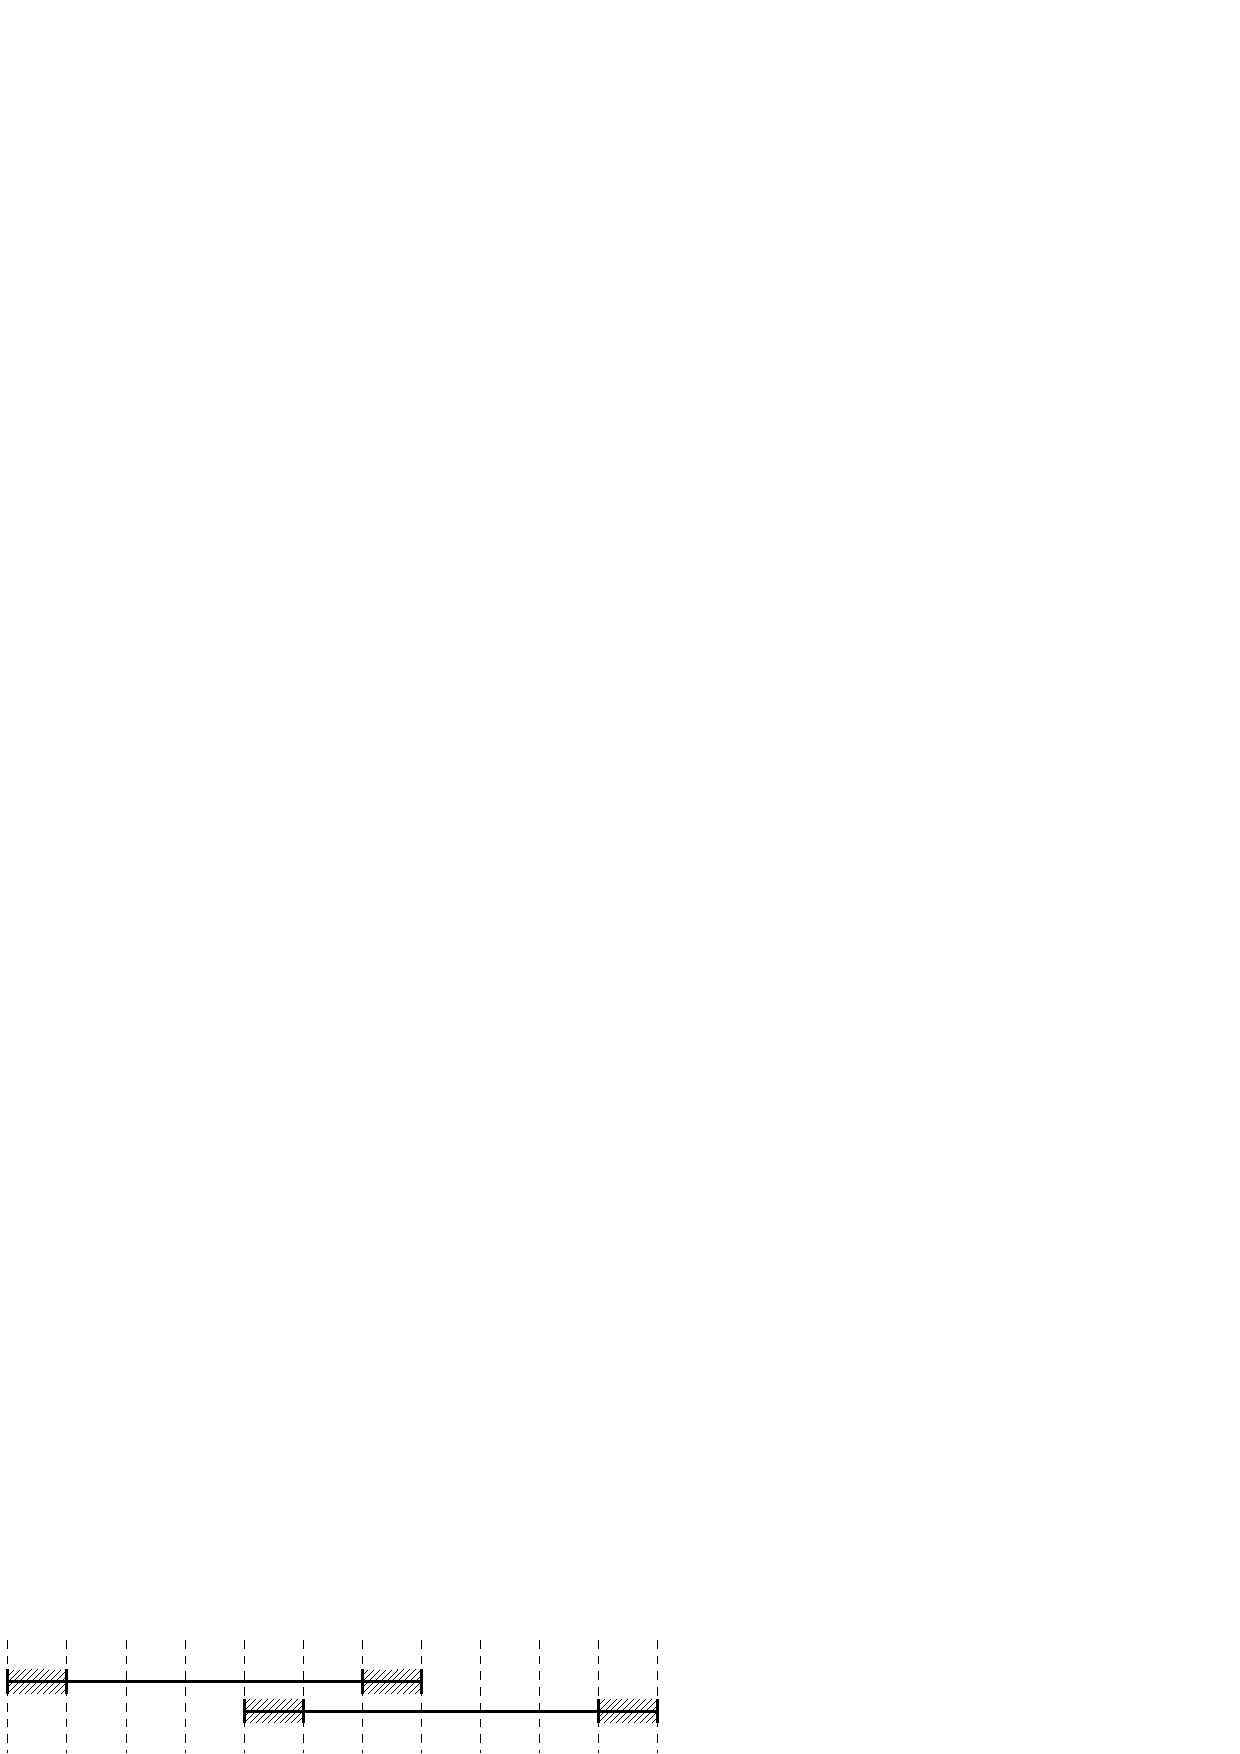
\includegraphics{figures/power/psds.fig.pdf}%
\end{picture}%
\setlength{\unitlength}{4144sp}%
%
\begingroup\makeatletter\ifx\SetFigFont\undefined%
\gdef\SetFigFont#1#2#3#4#5{%
  \reset@font\fontsize{#1}{#2pt}%
  \fontfamily{#3}\fontseries{#4}\fontshape{#5}%
  \selectfont}%
\fi\endgroup%
\begin{picture}(5364,1032)(-59,197)
\put(-44,1109){\makebox(0,0)[lb]{\smash{{\SetFigFont{10}{12.0}{\familydefault}{\mddefault}{\updefault}0}}}}
\put(1756,1109){\makebox(0,0)[lb]{\smash{{\SetFigFont{10}{12.0}{\familydefault}{\mddefault}{\updefault}32768}}}}
\put(3106,1109){\makebox(0,0)[lb]{\smash{{\SetFigFont{10}{12.0}{\familydefault}{\mddefault}{\updefault}57344}}}}
\put(4906,1109){\makebox(0,0)[lb]{\smash{{\SetFigFont{10}{12.0}{\familydefault}{\mddefault}{\updefault}90112}}}}
\end{picture}%

\end{center}
Here we see two of the time series from the first diagram above, each of
which is to be passed to \function{EPSearch()} for analysis.  To see why
the overlap between these two time series must be chosen as it is, refer to
the first diagram above to see where the greyed-out fifth analysis window
was to be placed.  That is where the first analysis window in the second
time series here will be placed.

Prior to looping over the data one noise PSD estimation length at a time,
the data is passed through a conditioning filter.  To account for edge
effects in the filter, an amount of data set by the command line option
\option{--filter-corruption} is dropped from the analysis at both the
begining and end of the time series.  The arrangement is shown in the
following diagram.
\begin{center}
\begin{picture}(0,0)%
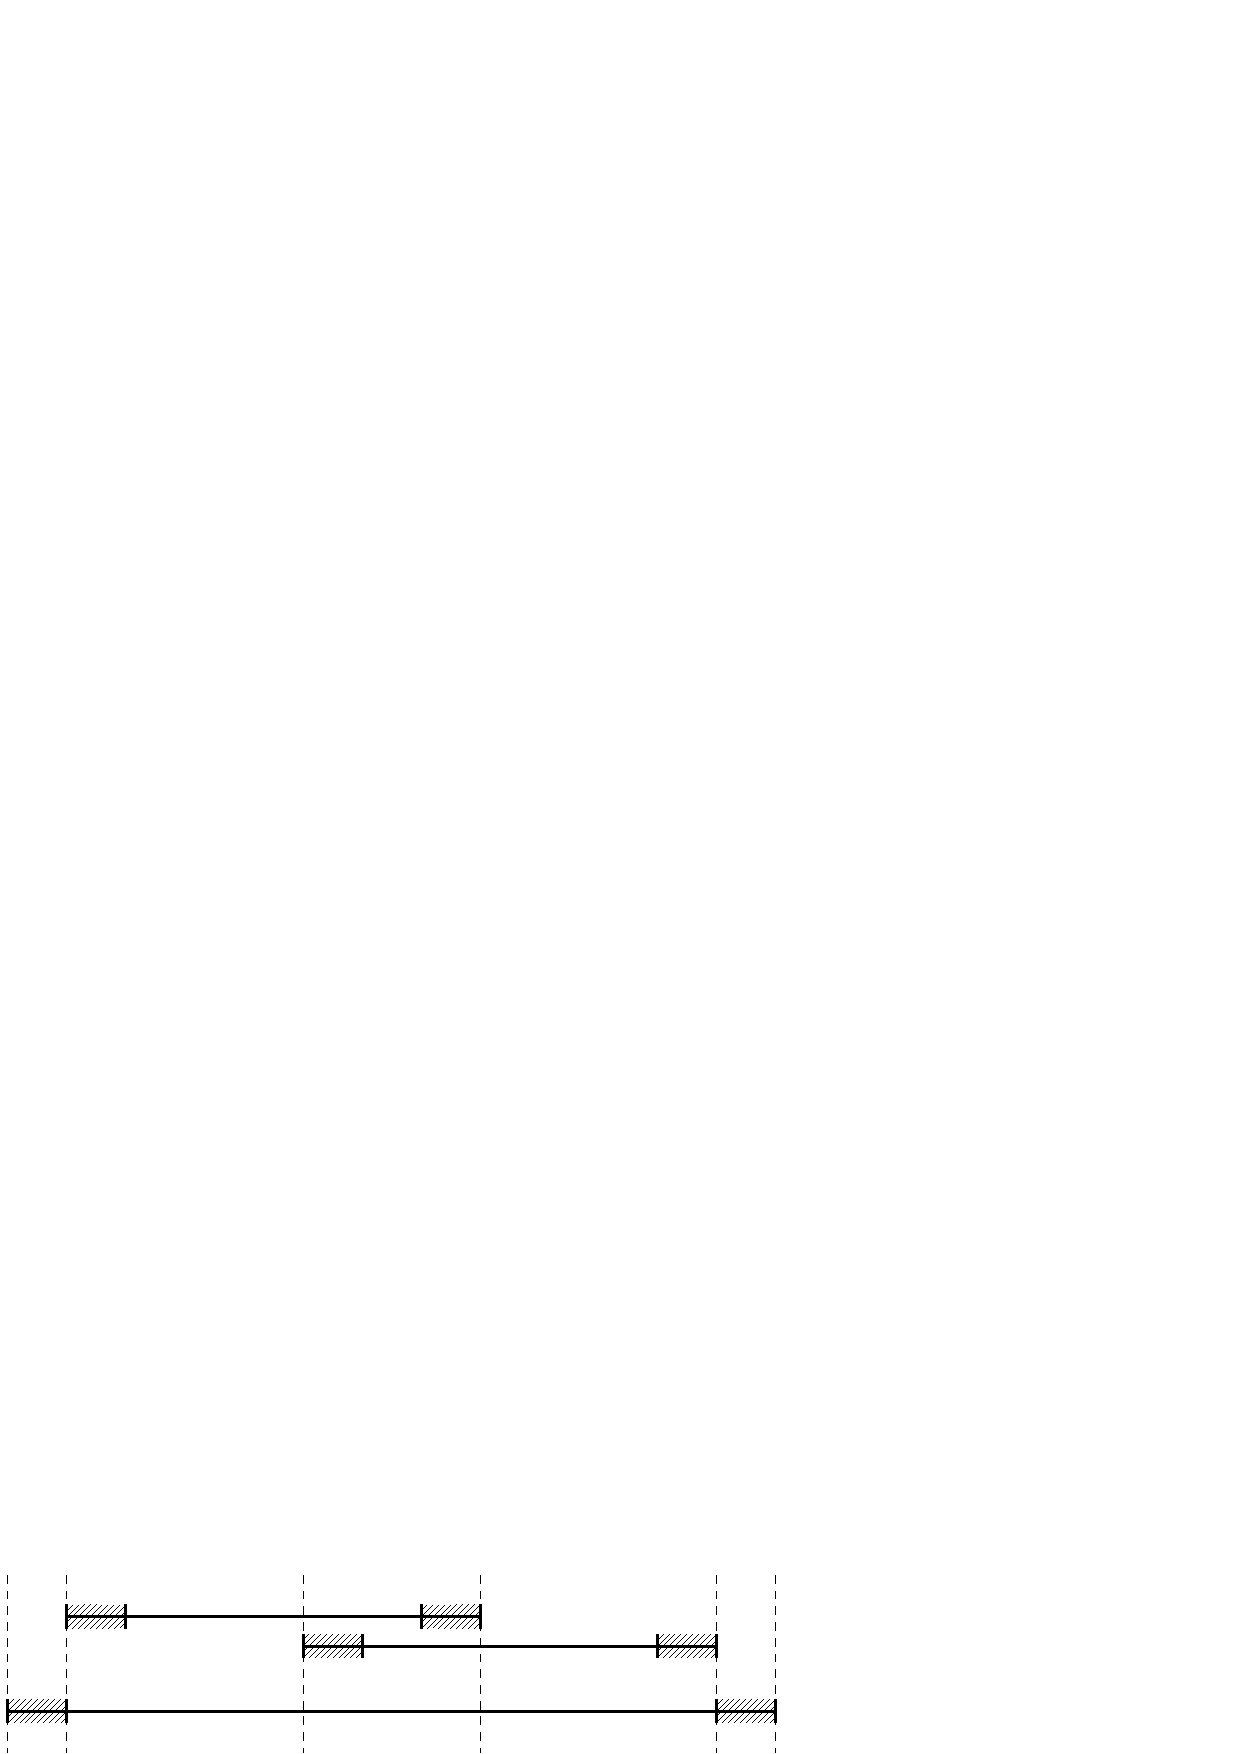
\includegraphics{figures/conditioning.fig.pdf}%
\end{picture}%
\setlength{\unitlength}{4144sp}%
%
\begingroup\makeatletter\ifx\SetFigFont\undefined%
\gdef\SetFigFont#1#2#3#4#5{%
  \reset@font\fontsize{#1}{#2pt}%
  \fontfamily{#3}\fontseries{#4}\fontshape{#5}%
  \selectfont}%
\fi\endgroup%
\begin{picture}(6341,1527)(-509,-298)
\put(-494,1109){\makebox(0,0)[lb]{\smash{{\SetFigFont{10}{12.0}{\familydefault}{\mddefault}{\updefault}0}}}}
\put(-44,1109){\makebox(0,0)[lb]{\smash{{\SetFigFont{10}{12.0}{\familydefault}{\mddefault}{\updefault}8192}}}}
\put(1756,1109){\makebox(0,0)[lb]{\smash{{\SetFigFont{10}{12.0}{\familydefault}{\mddefault}{\updefault}40960}}}}
\put(3106,1109){\makebox(0,0)[lb]{\smash{{\SetFigFont{10}{12.0}{\familydefault}{\mddefault}{\updefault}65536}}}}
\put(4906,1109){\makebox(0,0)[lb]{\smash{{\SetFigFont{10}{12.0}{\familydefault}{\mddefault}{\updefault}98304}}}}
\put(5356,1109){\makebox(0,0)[lb]{\smash{{\SetFigFont{10}{12.0}{\familydefault}{\mddefault}{\updefault}106496}}}}
\end{picture}%

\end{center}
The bottom-most line in this diagram represents the time series as read
into memory from disk.  In this example we have read 106496 samples into
memory, and after passing it through the conditioning filter 8192 samples
are dropped from the beginning and end of the series.  The remaining data
is then passed to \function{EPSearch()} 57344 samples at a time --- just as
was done in the earlier examples --- with appropriate overlaps.  In this
example, it happens that an integer number of overlaping noise PSD
intervals fits into the data that survives the conditioning.  In general
this will not be the case.  If the last noise PSD interval would extend
beyond the end of the time series, it is moved to an earlier time so that
its end is aligned with the end of the available data.

If more data needs to be analyzed than will fit in RAM at one time, we must
read it into memory and analyze it in pieces.  In doing this, we again want
the analysis windows in neighbouring read cycles to overlap one another in
the same manner that neighbouring analysis windows within a single noise
PSD interval overlap one another.  This will be assured if, in the diagram
above, the start of the next data to be read from disk is arranged so that
the first noise PSD interval to be analyzed within it starts at the correct
location relative to the last PSD interval analyzed from the previous read
cycle.  Consideration of the diagram above reveals that in order to meet
this condition, the next data to be read into memory should start $(2
\times \mbox{\parm{filter corruption}} + \mbox{\parm{window length}} -
\mbox{\parm{window shift}})$ samples prior to the end of the previous data
to have been read.


\subsection{Tuning the excess power pipeline}


The excess power search identifies time-frequency tiles as events when the 
probability of getting power in the tile from Gaussian noise alone
is below some particular threshold.  The search assumes no particular 
information about the gravitational wave signals other than the time
frequency ranges to search for,  so once those ranges are chosen the main 
tool to tune the pipeline is by tweaking the threshold.  The other parameter 
to test in the tuning procedure is the coincidence window.  Thus to 
summarize the parameters to tune in the excess power search are:
\begin{itemize}
\item maximum duration(seconds) of the tiles
\item maximum bandwidth of the tiles
\item probability thresholds on the individual instruments
\item the coincidence window
\end{itemize}
In the following sections we will go over the tuning of the different 
parameters in more details.


\subsubsection{Tuning the size of the tiles}
\label{section:tunetilesize}


The size(duration and bandwidth) of the tiles are largely guided by the
time-frequency content of the gravitational waves one is searching for.
  Here,  we describe the tuning procedure where we were concentrating 
on the search of the merger phase preceded by an inspiral phase.  As
mentioned before the physical parameters describing the merger phase
of a binary black hole coalescence are very poorly understood till
today.  However there are some rough estimates available in the literature 
which we will briefly describe here.  These will provide us a guideline
in choosing the parameters of our search pipeline. [FH:Flannagan and Hughes]

The process of coalescence can be roughly divided into three phases:
\begin{itemize}
\item Inspiral phase
\item Merger phase
\item Ringdown phase
\end{itemize}
The inspiral phase can be modelled accurately enough to use the match
filtering techniques to search for the waveforms, however for massive
black holes when there are not enough cycles left in the inspiral phase 
we have to rely on the merger phase for the detection of the coalescence.
According to the estimates of FH, binary black hole systems with total
mass $M \leq 30M_{\odot}$ are best searched for via their inspiral waves
while systems with $M > 30M_{\odot}$ must be searched via their
merger waves and/or their well understood ringdown waves.  

FH has estimated a conservative value for the merger frequency given
by 
\begin{equation}
f_{merge} = \frac{0.02}{M} \\
          = 205 Hz (\frac{20M_{\odot}}{M})
\label{eq:fmerge}
\end{equation}.
This is conservative in the sense that one can reasonably be sure that
numerically generated templates will not be needed before $f = f_{merger}$.
Now LIGO noise floor restricts the lowest frequency that can be searched 
for and in $S4$ this is $\approx 50 Hz$. Using \eqref{eq:fmerge} we 
then get that a binary system of maximum mass $\approx 80M_{\odot}$ 
can be searched for in $S4$.  However for a $80 M_{\odot}$ binary the 
number of cycles in the inspiral phase will be very small and since we
are interested in the coincidence of the mergers with the inspirals we
would like to restrict our search to a bit lower total mass.  Thus the 
mass range of the binary black holes that we decide to look at for the 
IB search is given by 
\begin{equation}
30 M_{\odot} < M \leq 70 M_{\odot}. 
\label{eq:massrange}
\end{equation}
Given this mass range let us now see what can we estimate about the 
expected frequency and duration of the merger signals. From 
\eqref{eq:fmerge} we get the approximte range of the merger frequencies:
\begin{equation}
58 Hz < f_{merge} \leq 140 Hz
\label{eq:frange}
\end{equation}
Now according to FH the high frequency shut off for the mergers are
roughly given by 
\begin{equation}
f_{qnr} = 1320 Hz (\frac{20M_{\odot}}{M})
\label{eq:fqnr}
\end{equation}
Thus if the assumed bandwidth of the merger signal is 
$\Delta f = f_{qnr} - f_{merge}$,  then for our mass range of 
interest we may expect the bandwidth to be of the order of few
hundred Hertz.  

The effective duration for the signals has also been roughly estimated
by FH to be:
\begin{equation}
50 M < T < 10 M
\label{eq:timerange}
\end{equation}
depending on the total spin of the binary system. If we consider
a coalescence where both the inspiraling black holes are nearly
maximally spinning, with their spins and the orbital angular momentum
nearly alligned then the merger may be expected to be long,  while
for non-spinning black holes the merger will be rather quick.  Thus 
given our mass range of interest (\eqref{eq:massrange}) the 
time duration of the expected signals whould be somewhere in the 
range:
\begin{equation}
17.2 ms < T < 1.5 ms
\label{eq:trange}
\end{equation} 
  
So given these estimates about the bandwidth and the duration of the 
signals of our main interest we choose the following parameters in our
search pipeline:
\begin{itemize}
\item Low frequency cutoff: $50 Hz$
\item Bandwidth: $1024 Hz$
\item Maximum duration of a tile: $125 ms$; we have set the duration 
a few times longer than the maximum duration in \eqref{eq:trange}
because of the uncertainty in the estimations related to the nature 
of the merger signals.
\item Maximum bandwidth of a tile: $128 Hz$; we have the bandwidth 
smaller than the estimated bandwidths for the merger signals since
because of the LIGO noise curve the prominent contribution to the 
power from the merger phase will be for a few hundred Hertz.
\end{itemize}
The last two parameters set the maximum duration and bandwith of 
a single tile in the search,  which does not preclude us from searching
for longer or broader signals since we can always sum up the power
from multiple tiles triggered by the particular signal. 
    

\subsubsection{Deciding on the probability thresholds}


We saw in Sec~\ref{section:tunetilesize} that the sizes of the tiles
are mainly guided by the rough expectations about the signals that 
we are interested in.  However, the threshold on the probability
of power in a tile is guided by the optimisation between the false 
rate and efficiency to a set of Monte Carlo simulations.  The idea
we usually follow is to choose a threshold which lowers the false rate 
maintaining the efficiency at an acceptable value.

To get a rough idea about the region where we start loosing significant 
amount of efficiency without an appreciable effect in lowering the false 
rate we estimate the efficiencies and the false rates for a number of 
thresholds. We have used $Q9$ Sine-Gaussian waveforms at $235 Hz $ to
perform the tuning and the confidence thresholds are
$\{-30.0, -35.0, -40.0, -45.0, -50.0, -55.0, -60.0, -65.0, -70.0, -80.0, 
-90.0, -100.0, -150.0, -200.0\}$. How the efficiency and the false rate 
depend on the thresholds are shown in Fig~\ref{fig:dt125df128tune}: 
\begin{figure}
\begin{center}
\resizebox{.9\linewidth}{!}{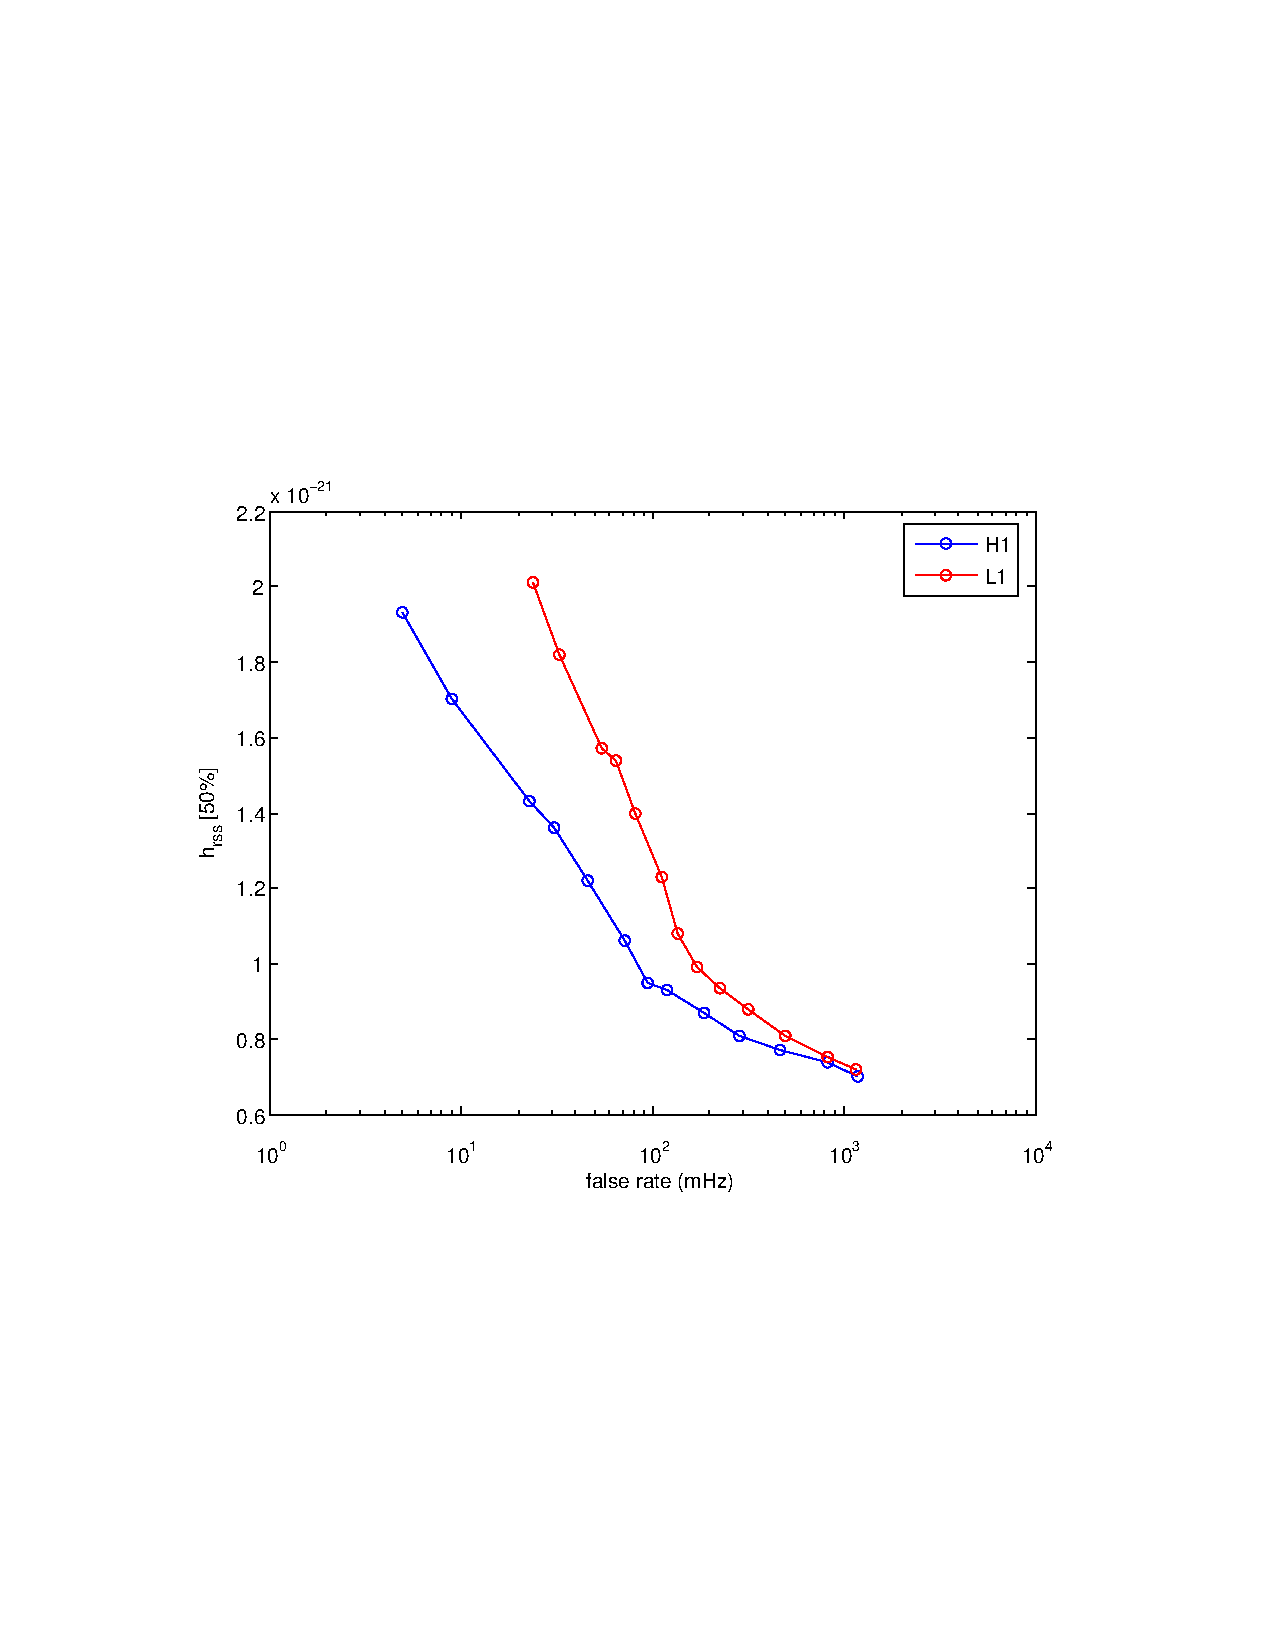
\includegraphics{figures/H1_L1_dt125_df128}}
\caption{Efficiency vs. False rate for different |thresholds|}
\label{fig:dt125df128tune}
\end{center}
\end{figure}
The circles on the curves show the values corresponding to different 
thresholds.  The maximum false rate and the best efficiency are obtained 
for the lowest |threshold|(30.0),  then as the |threshold| is increased
the false rate decreases while the efficiency gets worse. Around the 
|thresholds| of $50.0 - 60.0$ one may notice that for a very small 
decrease in false rate the efficiency gets a whole lot worse.  This gives 
us a rough idea that we should choose $ |threshold| < 60.0$.  However
one should be aware of the fact that tuning must be specific to the 
pipeline being run.  In our pipeline we have a coincidence step which
involves the burst triggers and the inspiral triggers and we are not
quite sure how many of the false triggers will survive that step. We
also plan to use the Hanford 2Km instrument in a coherent follow up at
the end of the pipeline which will also hopefully get rid off many of the
false triggers. However we would like to  
have a good estimate of the background distribution of triggers and so 
have a few surviviors at the end of the pipeline.  Keeping that 
in mind we decided to choose a looser threshold on the confidence 
probabilities. The thresholds we chose are 
\begin{itemize}
\item Threshold on H1: -38.0
\item Threshold on L1: -38.0; The instrument in Livingstone was less 
sensitive than the one in Hanford for the first half of the run but 
for the second half both the instruments had equal sensitivity.  So
we decided to have the same thresholds on both the instruments.
\end{itemize}      
These thresholds were so chosen so that the false rate after 
coincidence between H1 and L1 triggers is $\approx 2 mHz$ while 
the $ h_{rss}$ is $\approx 1.12e-21$.


\subsubsection{Choosing the coincidence window(W)}


The coincidence window(W) is given in milliseconds(ms).  When we 
have a trigger and want to find if there are triggers in the 
other instrument which are 
coincident with that we first pick the triggers which are within
$+/- W ms$ of the peak time of that trigger.  Once we find such a 
trigger we compare the time duration and frequency bandwidths and
if they overlap we mark them as coincident triggers. Ideally if a trigger 
is caused by a real gravitational wave signal then we expect that the
signal will trigger in the other instrument within $\approx +/- 10 ms$
since the light travel time between the two sites is that. But in the 
real analysis we may at times have to set longer windows because of 
errors creeping in from different sources like the timing inaccuracies 
of the search algorithm, errors in calibrations, etc..  In this step 
we choose the coincidence window for our pipeline.

We decided to choose the right window by doing a number of experiments
in the sense that we estimated the false rates and efficiencies
for a number of window sizes: $\{400 ms, 300ms, 200ms, 150 ms, 130ms,
110ms, 90ms, 70ms, 50ms, 30ms, 15ms\} $.  Fig~\ref{fig:tuneburcawindow}
shows the results of that experiment:   
\begin{figure}
\begin{center}
\resizebox{.9\linewidth}{!}{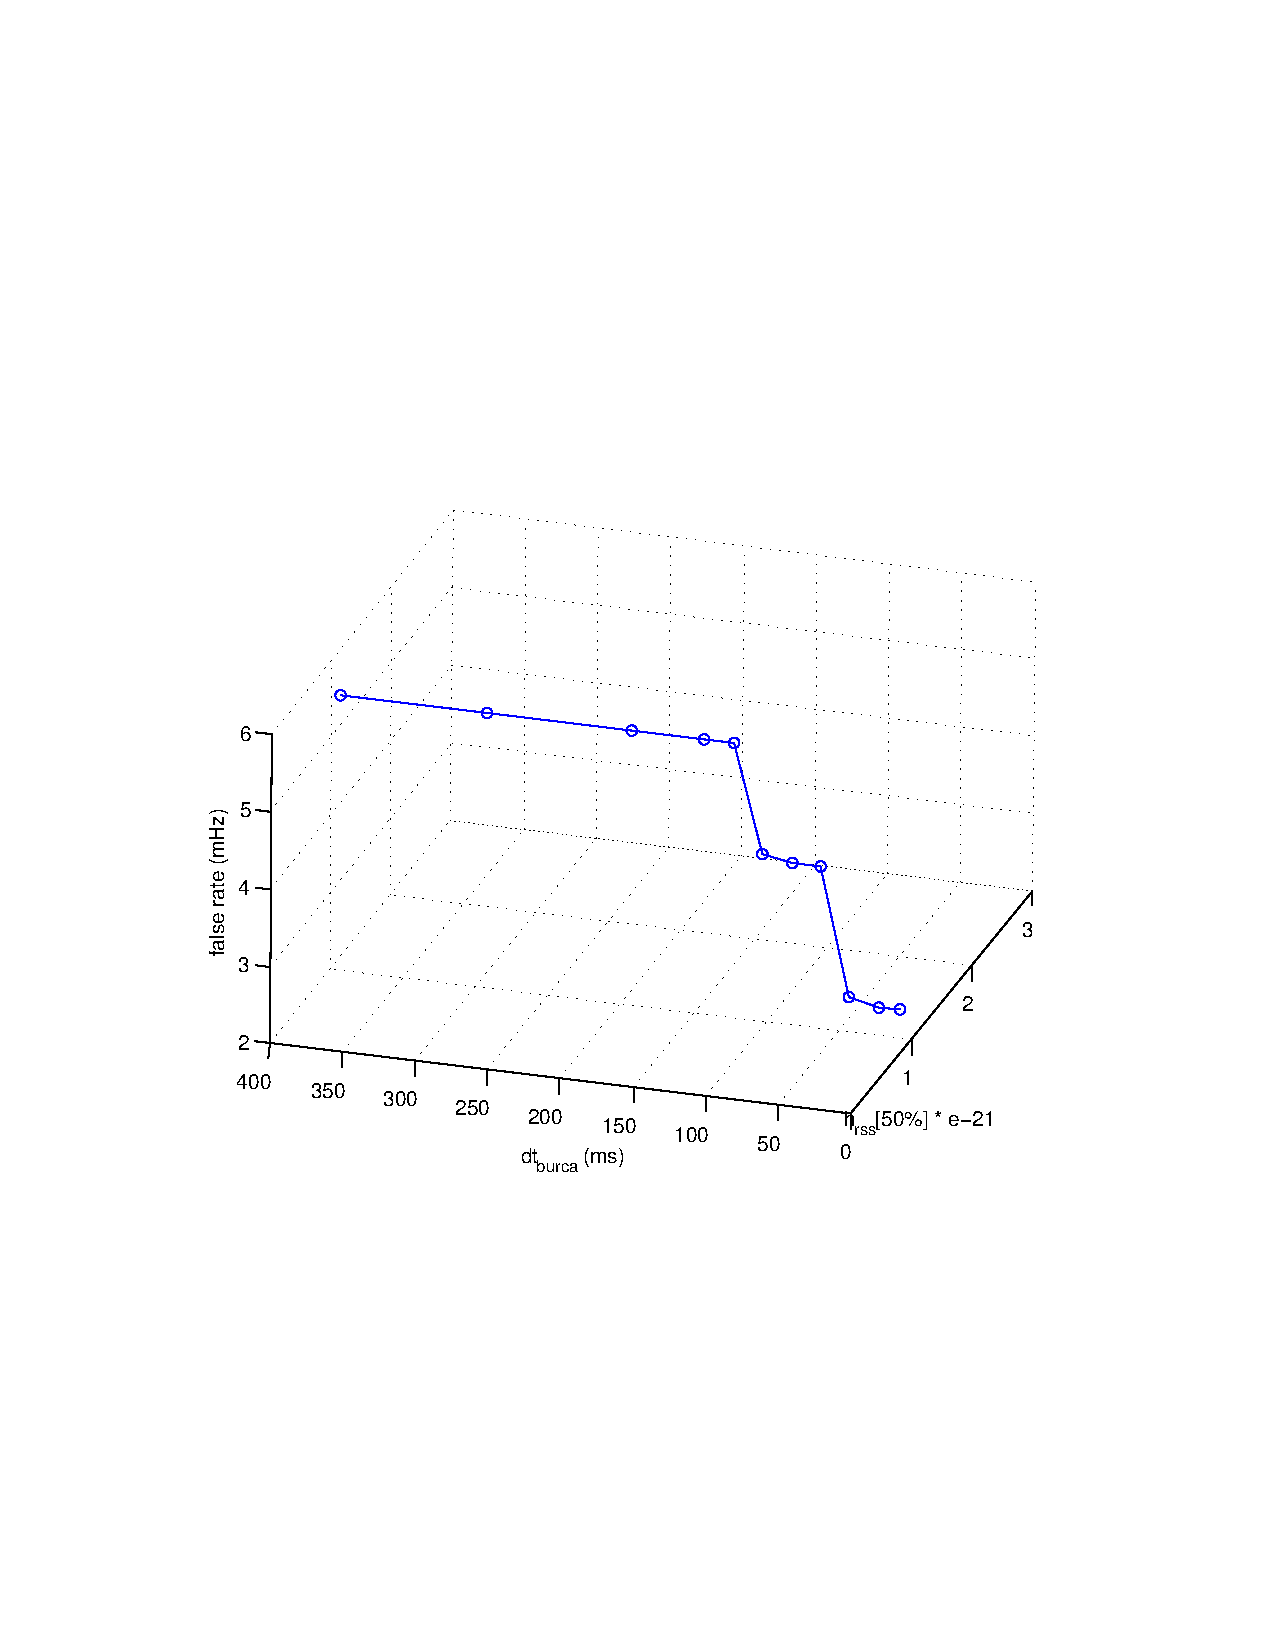
\includegraphics{figures/tune_burca_window}}
\caption{Efficiency vs. False rate for different coincidence windows}
\label{fig:tuneburcawindow}
\end{center}
\end{figure} 
From the Fig~\ref{fig:tuneburcawindow} we then see that the coincidence
window has no effect in the efficicency and some minimal effects on
the false rates. This implies that our time-frequency overlap criterion
in the coincidence step has made the window length a somewhat less 
important parameter for the coincidence. Allowing a margin of error 
from sources like calibration we therefore choose the window size to be
\begin{itemize}
\item Coincidence Window: 30 ms
\end{itemize}

Here we present a set of results from S4 using the parameters tuned
as decribed in the previous sections:
\begin{itemize}
\item Fig~\ref{fig:eventsvstimelag} shows the number of false events 
at each time lag.
\item Fig~\ref{fig:sg235q9eff} shows the efficiency of the pipeline to 
$Q9$ SineGaussians at $235 Hz$. The $h_{rss}$ 50 p.c. is at $1.12e-21$.
\item Fig~\ref{fig:eobeff} shows the efficiency of the pipeline to 
EOB waveforms. The $50 p.c.$ efficiency is at $66.5 Mpc$ effective distance.   
\end{itemize}.
\begin{figure}
\begin{center}
\resizebox{.9\linewidth}{!}{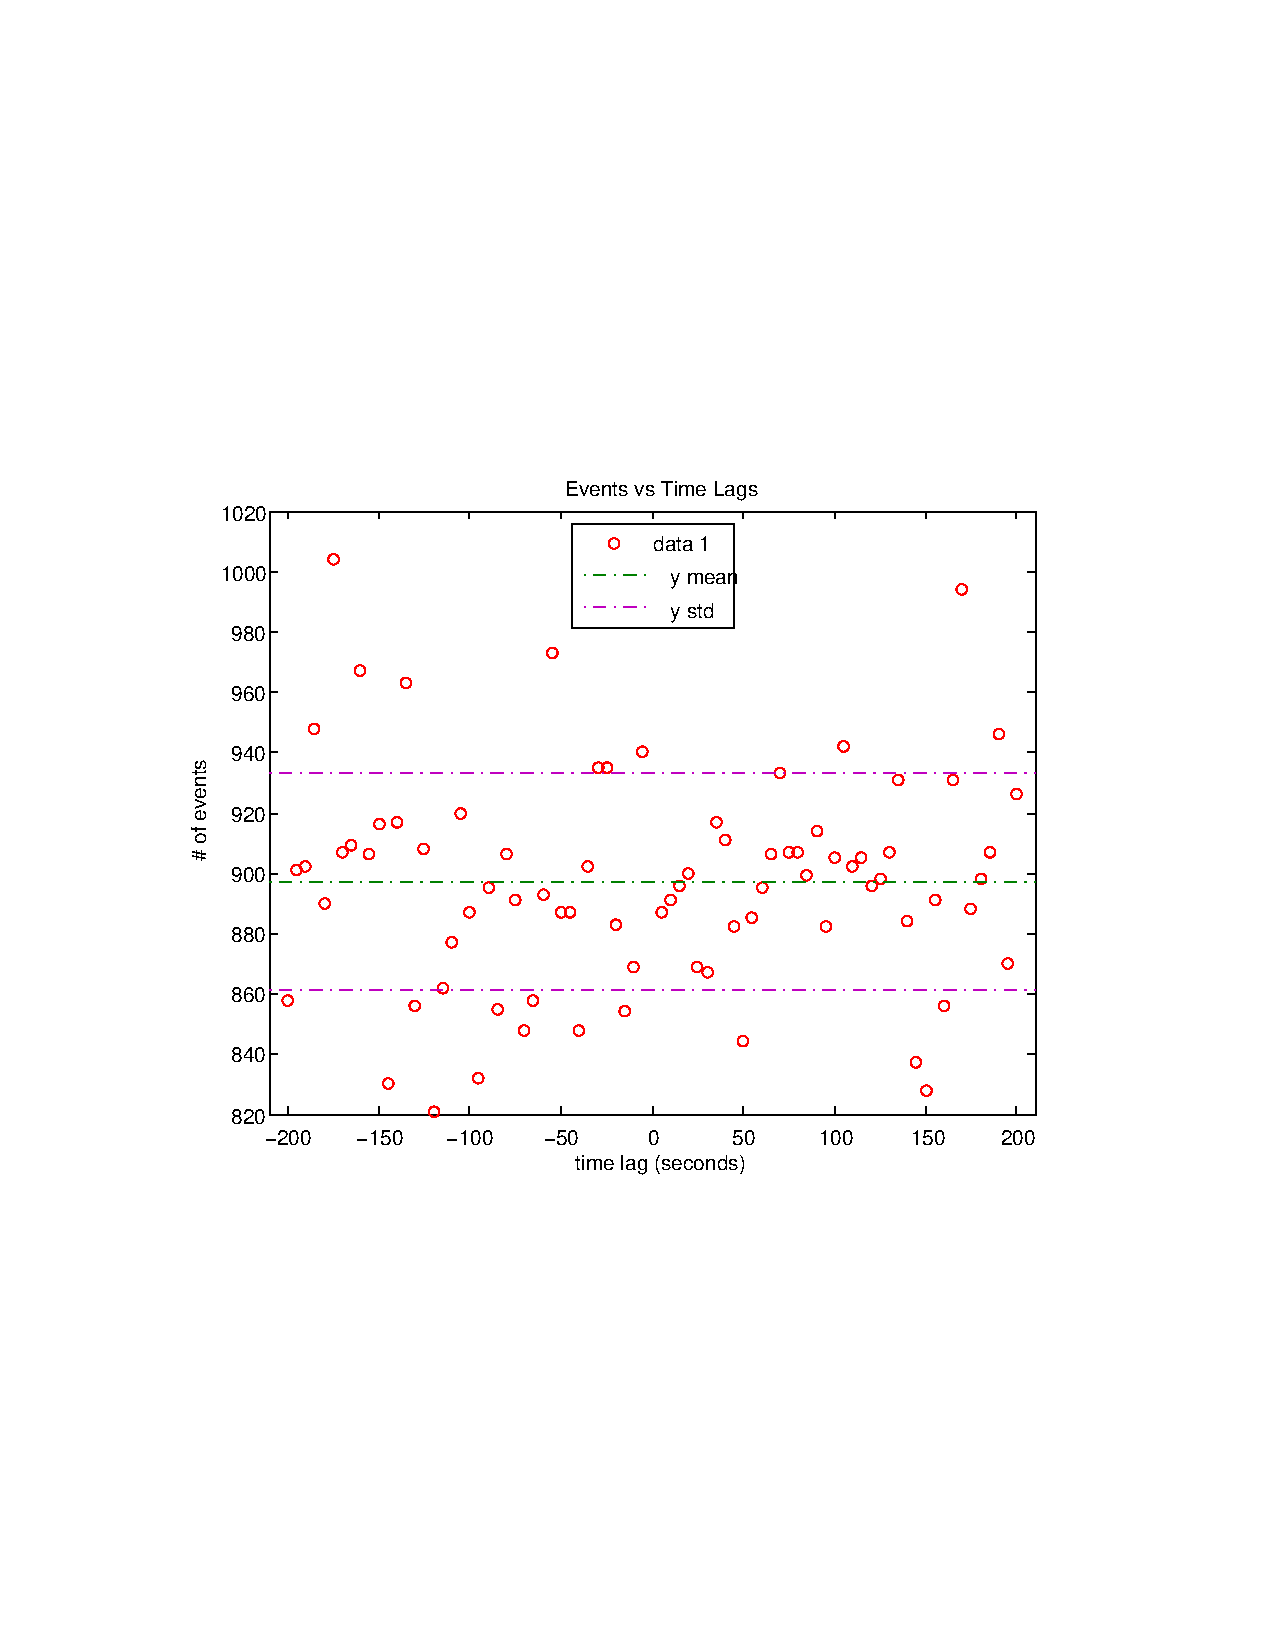
\includegraphics{figures/eventsvstimelag_20050829_1}}
\caption{No. of false triggers at different time lags}
\label{fig:eventsvstimelag}
\end{center}
\end{figure}

\begin{figure}
\begin{center}
\resizebox{.9\linewidth}{!}{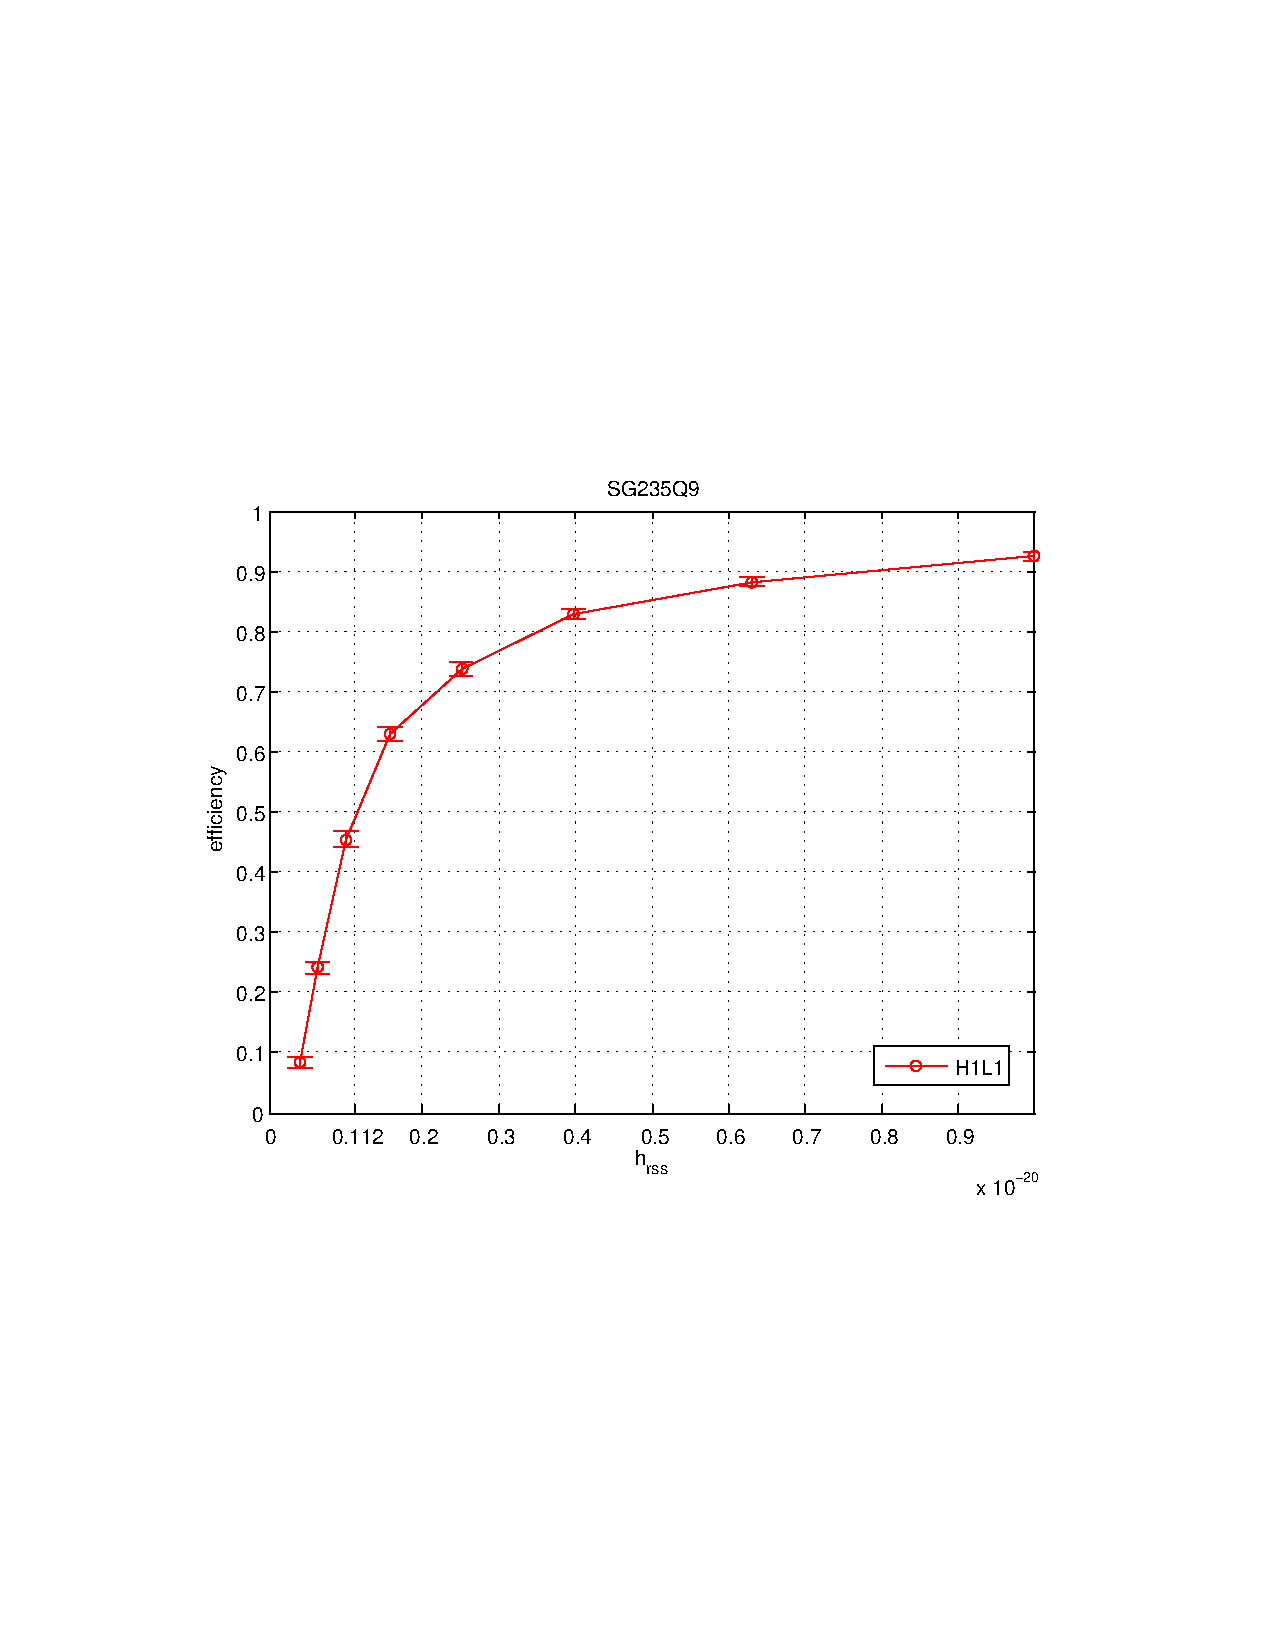
\includegraphics{figures/H1L1_eff_sg235q9_20050829_2.pdf}}
\caption{Efficiency to Q9 SineGausians at 235 Hz}
\label{fig:sg235q9eff}
\end{center}
\end{figure}

\begin{figure}
\begin{center}
\resizebox{.9\linewidth}{!}{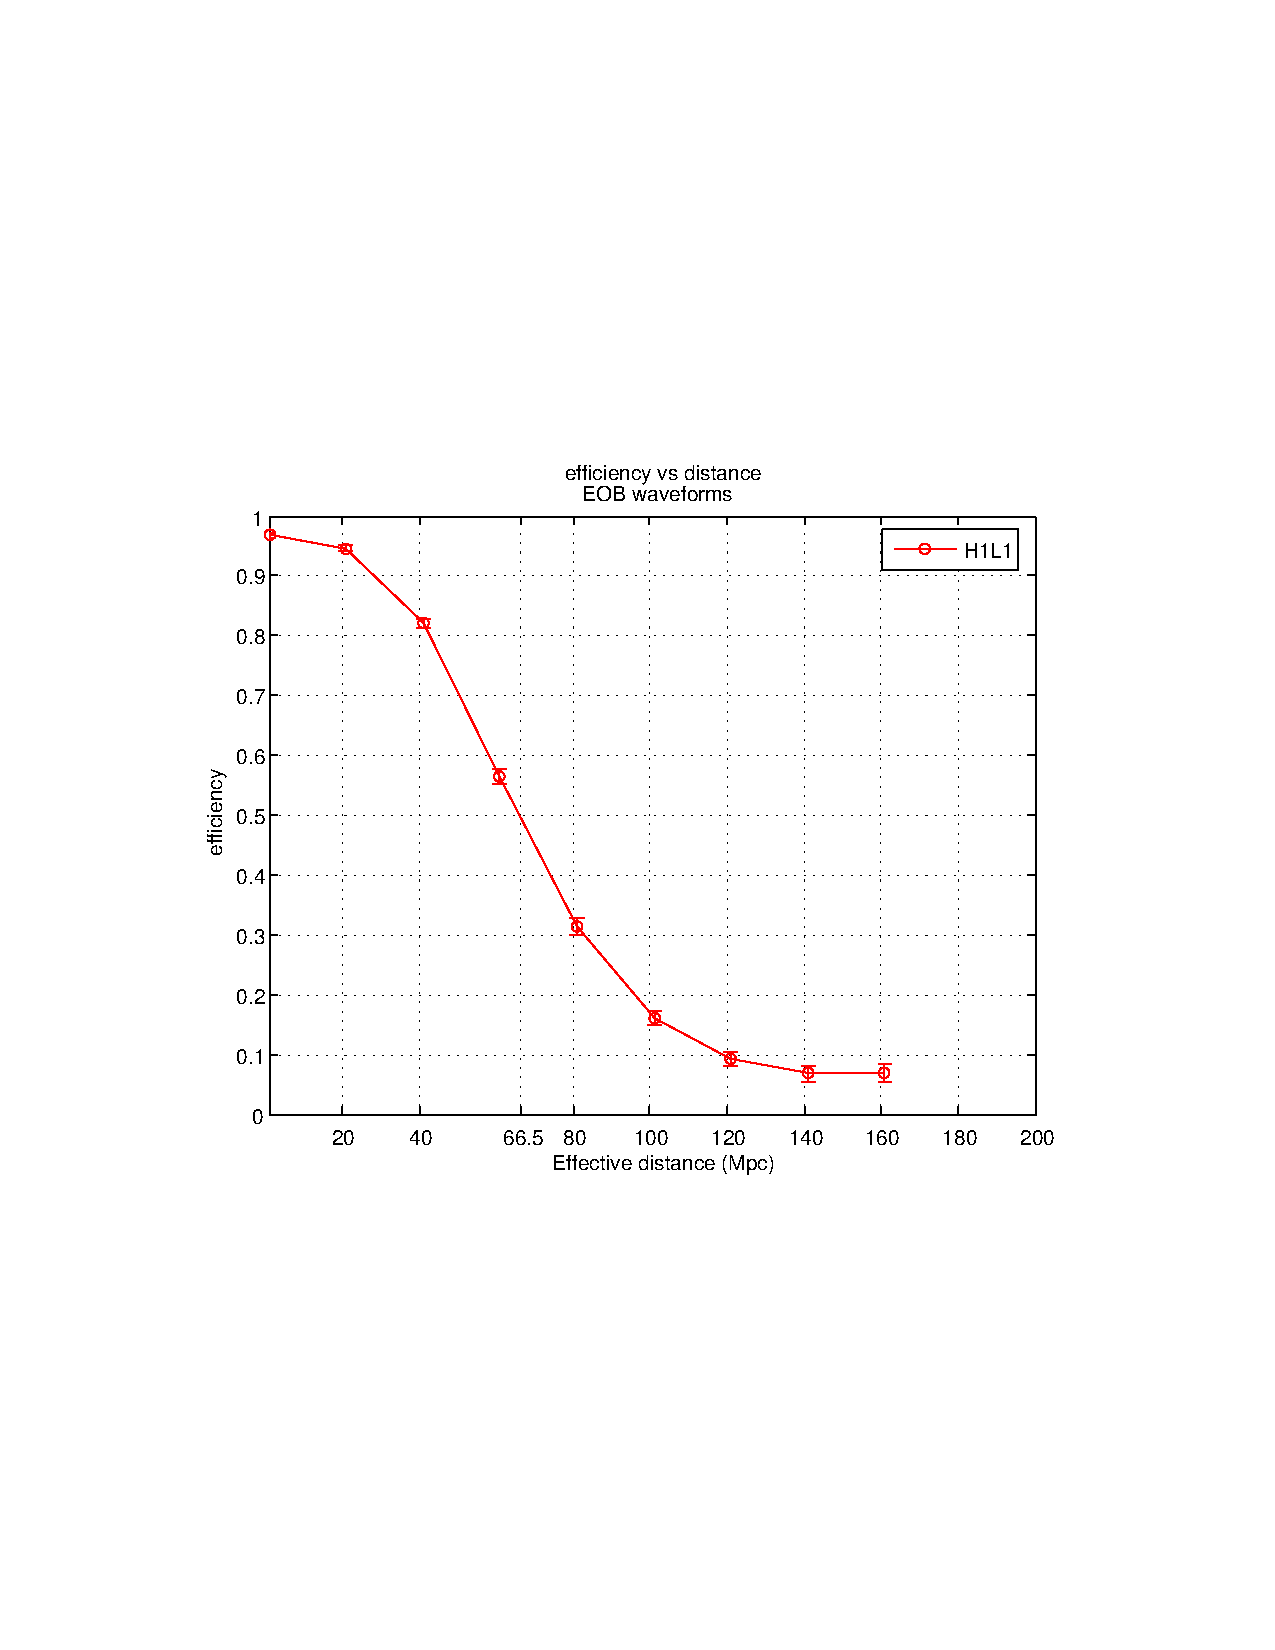
\includegraphics{figures/H1L1_eff_eob_20050829_3.pdf}}
\caption{Efficiency to EOB waveforms}
\label{fig:eobeff}
\end{center}
\end{figure}



\section{Program \prog{ligolw\_bucluster}}


\subsection{Clustering in Excess Power Search}


%
% FIXME: this section is obsolete
%

The excess power search is a multi-resolution analysis of the
time-frequency structure of the input time series.  A burst trigger is
identified if the probability of obtaining the excess power in a
time-frequency tile from Gaussian noise is smaller than some threshold
$\alpha$.   For large bursts in the data stream, many tiles can be
identified as triggers with different sizes and aspect ratios.   Hence when
the search over a particular segment is complete,   triggers have to be
clustered. 

The triggers are identified by a number of characteristic features like
start time,  peak time,  central frequency,  bandwidth,  excess power (the
excess compared to the power expected in Gaussian noise for the
corresponding time fequency volume)  and a confidence assosciated with this
measurement.  To do the clustering we first compare the peak times of the
triggers.  If the peak times are within an allowed range,  i.e. if
$|peaktime(trigger 1) - peaktime(trigger 2)| < dt$ where $dt$ is some
seconds,  we check whether the triggers  overlap in frequency.  If they
overlap,  we cluster them into one single trigger whose start time and
bandwidth are so chosen that they cover the time-frequency area which
includes the areas of the individual triggers.  The peak time of the
clustered trigger is equal to the peak time of that trigger which has more
excess power between the two.  Then we repeat the comparison but now
between the clustered trigger and another trigger.  If the peak times again
lie within the specified range and the frequencies overlap,  we modify,
otherwise we keep them as distinct triggers.  We repeat these steps until
there are no more distinct triggers which satisfy our criterion for
clustering.  The execess power of the cluster is the maximum of the
triggers involved in that particular cluster.

Top panel in Figure~\ref{fig:checkcluster}  shows a set of triggers before
clustering,  middle panel shows a set of clustered triggers when $dt$ was
chosen to be $10  nanosecs$ and the bottom panel shows the cluster when
$dt$ was $10  secs$. In the bottom panel there is only $1$ clustered
trigger and if one looks at the top panel this is expected because all the
peak  times of the triggers(before clustering)  lie within $10  secs$ of
each other.
\begin{figure}
\centering
\resizebox{.9\linewidth}{!}{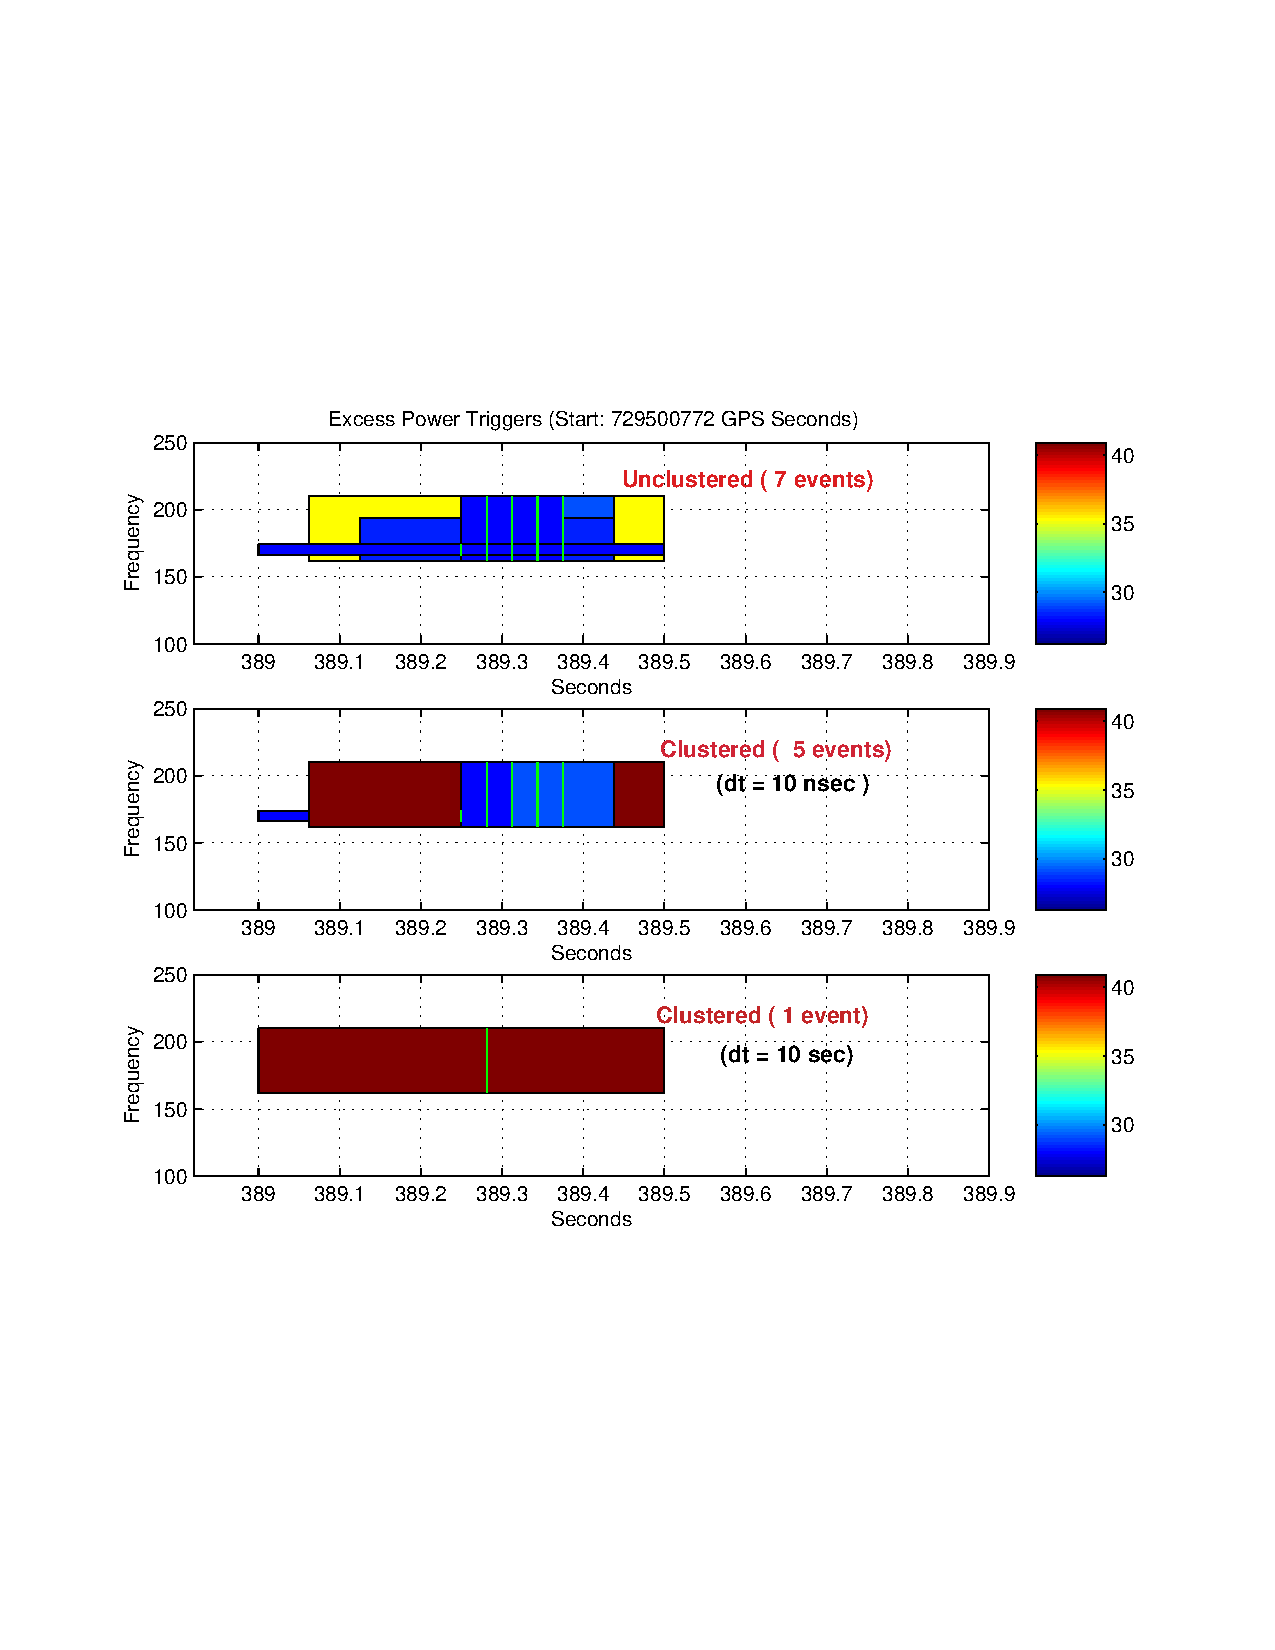
\includegraphics{figures/checkclustering_dt10nsec10sec}}
\caption{Clustering in Excess Power}
\label{fig:checkcluster}
\end{figure}

To understand this better let us look at the triggers themselves:

\vspace{0.1 in}

\begin{tabular}{||l|l|l|l|l|l|l|lr||} \hline
no. & start time(sec) & peak time(sec) & duration(sec) & central freq(Hz) & bandwidth(Hz) & snr \\ \hline
1 &729501161.0  & 729501161.25  & 0.5     & 170  & 8   & 66.121277 \\ \hline
2 &729501161.125  & 729501161.28125  & 0.3125  & 186  & 48  & 123.3495 \\ \hline
3 &729501161.0625  & 729501161.28125  & 0.4375  & 186  & 48  & 120.2974 \\ \hline
4 &729501161.125 &729501161.28125 &0.3125 &178 &32 &82.274979 \\ \hline
5 &729501161.25 &729501161.3125 &0.125 &186 &48 &72.011459  \\ \hline
6 &729501161.25 &729501161.34375 &0.1875 &186 &48 & 92.914597 \\ \hline
7 &729501161.3125 &729501161.375 &0.125 & 186 &48 & 74.42984 \\ \hline
\end{tabular}

\vspace{0.1 in} 

The table above contains the set of triggers before clustering while   
the table below contains the $5$ clustered events when $dt$ 
was $10 nanosec$.

\vspace{0.1 in}

\begin{tabular}{||l|l|l|l|l|l|l|lr||} \hline
no. & start time(sec) & peak time(sec) & duration(sec) & central freq(Hz) & bandwidth(Hz) & snr \\ \hline
1 &729501161.0 &729501161.25 &0.5 &170 &8 & 66.121277 \\ \hline
2 &729501161.0625 &729501161.28125 &0.4375 &186 &48 &123.3495 \\ \hline
3 &729501161.25 &729501161.34375 &0.1875 &186 &48 &92.914597 \\ \hline
4 &729501161.25 &729501161.3125 &0.125 &186 &48 &72.011459 \\ \hline
5 &729501161.3125 &729501161.375 &0.125 &186 &48 &74.42984 \\ \hline 
\end{tabular}

\vspace{0.1 in}

Thus from this set of clustered triggers it is quite clear what we have been 
discussing till now.



\section{Program \prog{lalapps\_binj}}
\label{program:lalapps-binj}


\begin{entry}
\item[Name]
\prog{lalapps\_binj} --- produces burst injection data files.

\item[Synopsis]
\prog{lalapps\_binj} \newline \hspace*{0.5in}
[\option{--help}] \newline \hspace*{0.5in}
\option{--gps-start-time}~\parm{tstart} \newline \hspace*{0.5in}
\option{--gps-end-time}~\parm{tend} \newline \hspace*{0.5in}
[\option{--time-step}~\parm{tstep}] \newline \hspace*{0.5in}
[\option{--seed}~\parm{seed}] \newline \hspace*{0.5in}
[\option{--waveform}~\parm{wave}] \newline \hspace*{0.5in}
[\option{--population}~\parm{name}] \newline \hspace*{0.5in}
[\option{--freq-dist}~\parm{name}] \newline \hspace*{0.5in}
[\option{--flow}~\parm{flow}] \newline \hspace*{0.5in}
[\option{--fhigh}~\parm{fhigh}] \newline \hspace*{0.5in}
[\option{--deltaf}~\parm{deltaf}] \newline \hspace*{0.5in}
[\option{--quality}~\parm{quality}] \newline \hspace*{0.5in}
[\option{--tau}~\parm{tau}] \newline \hspace*{0.5in}
[\option{--strain-dist}~\parm{name}] \newline \hspace*{0.5in}
[\option{--strain-scale-min}~\parm{value}] \newline \hspace*{0.5in}
[\option{--strain-scale-max}~\parm{value}] \newline \hspace*{0.5in}
[\option{--max-distance}~\parm{max-distance}] \newline \hspace*{0.5in}
[\option{--min-distance}~\parm{min-distance}] \newline \hspace*{0.5in}
[\option{--simwaveform-duration}~\parm{simwaveform-duration}] \newline \hspace*{0.5in}
[\option{--simwaveform-min-number}~\parm{simwaveform-min-number}] \newline \hspace*{0.5in}
[\option{--simwaveform-max-number}~\parm{simwaveform-max-number}] \newline \hspace*{0.5in}
[\option{--usertag}~\parm{tag}]

\item[Description] 
\prog{lalapps\_binj} generates a number of burst parameters suitable for
using in a Monte Carlo injection to test the efficiency of a burst search.
The various parameters (detailed below) are specified on the command line
or can be randomly chosen in a manner appropriate for an burst upper limit
search.

\prog{lalapps\_binj} produces an injection set following one of two sky
disitributions:  a set of injections from point sources
uniformly-distributed over the sky with uniformly-distributed linear
polarizations, or a set of injections located directly above each
observatory with optimally-oriented linear polarizations.  Which set is
produced is selected by the \option{--population} option.

Injections are produced with various strains, and one of several strain
distributions can be selected with the \option{--strain-dist} parameter.
Some strain distributions require a ``min'' and or a ``max'' parameter, for
example in the case of logarithmically-distributed \(h_{\mathrm{rss}}\) one
needs to specify the smallest and largest values of \(\log_{10}
h_{\mathrm{rss}}\).  These parameters are set using the
\option{--strain-scale-min} and \option{--strain-scale-max} command line
arguments.  The following table lists the strain distributions, and the
meaning of the ``min'' and ``max'' parameters for each.
\begin{center}\begin{tabular}{p{3cm}ccc}
\hline\hline
Description & \option{--strain-dist} & \option{--strain-scale-min} &
\option{--strain-scale-max} \\
\hline
Constant \(h_{\mathrm{peak}}\) & \texttt{consthpeak} & \(h_{\mathrm{peak}}\) & n/a \\
Constant \(h_{\mathrm{rss}}\) & \texttt{consthrss} & \(h_{\mathrm{rss}}\) & n/a \\
Randomly select one of several preset values of \(h_{\mathrm{peak}}\) & \texttt{hpeakpresets} & n/a & n/a \\
Uniformly-distributed \(\log_{10} h_{\mathrm{peak}}\) & \texttt{loghpeak} & \(\min \log_{10} h_{\mathrm{peak}}\) & \(\max \log_{10} h_{\mathrm{peak}}\) \\
Uniformly-distributed \(\log_{10} h_{\mathrm{rss}}\) & \texttt{loghrss} & \(\min \log_{10} h_{\mathrm{rss}}\) & \(\max \log_{10} h_{\mathrm{rss}}\) \\
Uniformly-distributed \(\log_{10} (h_{\mathrm{rss}} \Delta t)\) & \texttt{loghrss-t} & \(\min \log_{10} (h_{\mathrm{rss}} \Delta t)\) & \(\max \log_{10} (h_{\mathrm{rss}} \Delta t)\) \\
\hline\hline
\end{tabular}\end{center}

One of several frequency distributions can be chosen.  If the waveform is
set to \texttt{StringCusp}, then a frequency distribution appropriate for
that source is selected.  Otherwise the user can choose an arithmetic
frequency progression, a geometric frequency progression, or a
logarithmically-uniform random frequency distribution.

The output of this program  is  a  list  of  the  injected events, starting
at  the specified start time, ending at the specified end time, and
containing one set  of burst parameters every specified time step.  The
output is written to a file name in the standard burst pipeline format:
\begin{center}
\begin{verbatim}
        HL-INJECTIONS_USERTAG_SEED-GPSSTART-DURATION.xml
\end{verbatim}
\end{center}
where \verb$USERTAG$ is \parm{tag} as specfied on the command line,
\verb$SEED$ is the  value  of  the random number seed chosen and
\verb$GPSSTART$ and \verb$DURATION$ describes the GPS time interval that
the file covers. The file is in the standard LIGO lightweight XML format
containing a \texttt{sim\_burst} table that describes the injections.  This
table is described in the LAL \texttt{tools} package under
\texttt{LIGOMetadataTables.h} header.  

If a \option{--user-tag} is not specified on the command line, the
\texttt{\_USERTAG} part of the filename will be omitted.

\item[Options]\leavevmode
\begin{entry}
\item[\option{--help}] Print a help message.

\item[\option{--gps-start-time} \parm{tstart}]
Required.  Start time of the injection data to be created.

\item[\option{--gps-end-time} \parm{tend}]
Required.  End time of the injection data to be created.

\item[\option{--time-step} \parm{tstep}]
Optional. Sets the time step interval between injections. The injections
will occour at \parm{tstep}$/\pi$ second intervals. Defaults to $2630/\pi$.

\item[\option{--seed} \parm{seed}]
Optional. Seed the random number generator with the integer \parm{seed}.
Defaults to $1$.

\item[\option{--population} \parm{name}]
The population of injections to synthesize.  Select one of:
\begin{itemize}
\item \texttt{uniform\_sky}
\item \texttt{zenith}
\end{itemize}
The default is \texttt{uniform\_sky}, which produces a set of point-source
injections uniformly distributed over the sky with uniformly distributed
linear polarization.  \texttt{zenith} produces a set of injections incident
from directly above each observatory and optimially-oriented for each
(think of this as a burst in the form of an inwardly-directed spherical
shell centred on the geocenter, with optimal polarization at each
observatory).

\item[\option{--freq-dist} \parm{name}]
Optional.  If not doing string injections (by setting
\option{--waveform=StringCusp}), use this to select a frequency
distribution.  Allowed values are \option{monoarithmetic} for a
monotonically increasing arithmetic progression, \option{monogeometric} for
a monotonically increasing geometric progression, or \option{randgeometric}
for a sequence of logarithmically-distributed random frequencies.
\emph{Note}:  the \option{randgeometric} sequence is a variant of the
\option{monogeometric} sequence with each injection displaced from the
nominal frequency by a random amount.  To avoid biasing the noise estimate
by having two injections occur at nearly the same frequency, a larger
\option{--fratio} should be used with this sequence.

\item[\option{--flow} \parm{flow}]
Optional.  The code can generate injections at multiple frequencies.  This
option sets the first frequency used in that case.  Default value is 150
Hz.

\item[\option{--fhigh} \parm{fhigh}]
Optional.  Only generate injections with frequencies below \parm{fhigh}.
Default value is 1000 Hz.

\item[\option{--deltaf} \parm{deltaf}]
Optional.  The linear spacing between frequencies used to make
injections.  Default value is 0 Hz.

\item[\option{--waveform} \parm{wave}]
Optional.  Default is \texttt{SineGaussian}.   The string \parm{wave} will
be written into the \texttt{waveform} column of the \texttt{sim\_burst}
table output. This is used by the burst code to determine which type of
waveforms it should inject into the data.  Types implemented in LAL inject
package are:
\begin{description}
\item[\texttt{SineGaussian}]  Inject a sine-Gaussian waveform defined by
\begin{eqnarray}
A_+(t) &=& h_0 \exp[ - (t-t_0)^2/ \tau^2 ] \sin[ 2 \pi f_0 (t-t_0)] \\
A_\times(t) &=& 0
\end{eqnarray}

\item[\texttt{CosGaussian}]  Inject a cos-Gaussian waveform defined by
\begin{eqnarray}
A_+(t) &=& h_0 \exp[ - (t-t_0)^2/ \tau^2 ] \cos[ 2 \pi f_0 (t-t_0)] \\
A_\times(t) &=& 0
\end{eqnarray}
\end{description}

\item[\option{--tau} \parm{tau}]
Optional.  The decay-time $\tau$ for sine-gaussian,  gaussian,  ringdown
and ring-up waveforms.

\item[\option{--quality} \parm{quality}]
Optional.  The quality factor for sine-gaussian,  gaussian,  ringdown and
ring-up waveforms.    This option overrides the decay-time \parm{tau} and
recalculates the duration for each waveform using the formula
$$ 
\tau = \frac{\textsc{quality} }{ \sqrt{2} \pi f_0 }
$$
where $f_0$ is the frequency of the injection.

\item[\option{--strain-dist} \parm{name}]
Required.  Select the strain amplitude distribution.  See the table in the
Description section above for more information.

\item[\option{--strain-scale-min} \parm{value}]
Optional.  Used to set the minimum of the distribution selected with
\option{--strain-scale}.  The meaning of the value set with this parameter
depends on the distribution chosen.

\item[\option{--strain-scale-max} \parm{value}]
Optional.  Used to set the maximum of the distribution selected with
\option{--strain-scale}.  The meaning of the value set with this parameter
depends on the distribution chosen.

\item[\option{--user-tag} \parm{string}]
Optional. Set the user tag for this job to be \parm{string}. May also be
specified on the command line as \option{-userTag} for LIGO database
compatibility.

\item[\option{--max-distance} \parm{distance}]
Optional.  This is used when one wants to inject simulated Inspiral$+$Burst$+$Ringdown 
waveforms.  This specifies the maximum distance in Kpc that a source can be placed at.
This should be used with the \option{--min-distance}.

\item[\option{--min-distance} \parm{distance}]
Optional.  This is used when one wants to inject simulated Inspiral$+$Burst$+$Ringdown 
waveforms.  This specifies the minimum distance in Kpc that a source can be placed at.
This should be used with the \option{--max-distance}.

\item[\option{--d-distr} \parm{distribution number}] 
Optional.  This is used when the maximum and minimum distribution options are used.
 This should be an integer number and depending on the number different distance
distributions can be used while placing the sources.  

\item[\option{--simwaveform-duration} \parm{simwaveform-duration}]
Optional.  This specifies the duration in seconds of the frames containing the simulated 
waveforms.

\item[\option{--simwaveform-min-number} \parm{simwaveform-min-number}] 
Optional.  This specifies the minimum number of the simulated waveforms to be injected.

\item[\option{--simwaveform-max-number} \parm{simwaveform-max-number}] 
Optional.  This specifies the maximum number of the simulated waveforms to be injected.  
\end{entry}

\item[Example]
\begin{verbatim}
lalapps_binj \
--gps-start-time 794063160 \
--gps-end-time 794063610.5 \
--time-step 200 \
--flow 70.0 \
--fhigh 2118.0 \
--fratio 1.17629327749 \
--quality 8.89 \
--strain-dist consthpeak
--strain-scale-min 6.0e-20 \
--seed 45
\end{verbatim}

\item[Author] 
Jolien Creighton, Patrick Brady, Duncan Brown, Saikat Ray-Majumder, Kipp
Cannon
\end{entry}

 
\section{Running the power code under Condor}


%
% FIXME: this section is obsolete
%

This section is under construction!


\section{Program \prog{lalapps\_power\_pipe}}


\begin{entry}

\item[Name]
\prog{lalapps\_power\_pipe} --- builds a one/two/three interferometer excess-power
search DAG   

\item[Synopsis]
\prog{lalapps\_power\_pipe} \newline \hspace*{0.5in}
[\option{-h, --help}] \newline \hspace*{0.5in}
[\option{-v, --version}] \newline \hspace*{0.5in}
[\option{-u, --user-tag}~\parm{tag}] \newline \hspace*{0.5in}
[\option{-d, --datafind}] \newline \hspace*{0.5in}
[\option{-r, --power}] \newline \hspace*{0.5in}
[\option{-H, --ifo\_h1}] \newline \hspace*{0.5in}
[\option{-K, --ifo\_h2}] \newline \hspace*{0.5in}
[\option{-L, --ifo\_l}] \newline \hspace*{0.5in}
[\option{-c, --makeinjfiles}] \newline \hspace*{0.5in}
[\option{-j, --injections}~\parm{injection type}] \newline \hspace*{0.5in}
[\option{-m, --mdcinjections}] \newline \hspace*{0.5in}
[\option{-b, --coincidence}] \newline \hspace*{0.5in}
[\option{-t, --triplecoincidence}] \newline \hspace*{0.5in}
[\option{-s, --timeslides}] \newline \hspace*{0.5in}
[\option{-p, --playground-only}] \newline \hspace*{0.5in}
[\option{-P, --priority}~\parm{prio}] \newline \hspace*{0.5in}
\option{-f, --config-file}~\parm{file} \newline \hspace*{0.5in}
\option{-l, --log-path}~\parm{path}

\item[Description] 
\prog{lalapps\_power\_pipe} builds an excess power search DAG suitable for
running at the various LSC Data Grid sites.   The script requires a
configuration file.   An example file can be found in
\texttt{\$LALPREFIX/share/lalapps/power\_pipe.ini}.   Arguments to be
passed to the search code are supplied in this file and used the DAG
construction.  This is a standard python format configuration file.

\item[Options]\leavevmode
\begin{entry}

\item[\option{--help}] Prints the usage information

\item[\option{--user-tag} \parm{tag}]   The tag for the job.  This will
override the value set in the ini file

\item[\option{--datafind}] run LSCdataFind as part of the DAG to create the
cache files for each science segment

\item[\option{--power}] run \prog{lalapps\_power} on the data.  To run
the power jobs one has to specify the ifo or the combination of ifos.  This
can be specified by a combination of the options \option{--ifo\_h1},
 \option{--ifo\_h2} and \option{--ifo\_l}.  

\item[\option{--ifo\_h1}] run \prog{lalapps\_power} on the data from H1

\item[\option{--ifo\_h2}] run \prog{lalapps\_power} on the data from H2

\item[\option{--ifo\_l}] run \prog{lalapps\_power} on the data from L1

If one wants to run on both H1 and H2 data then the options \option{--ifo\_h1}
and \option{--ifo\_h2} have to be specified with \option{--power} and 
similarly for other combinations.  For example if one then wants to run on 
all of H1,  H2 and L1 data then all the three options,  \option{--ifo\_h1},
 \option{--ifo\_h2},  \option{--ifo\_l} have to be specified with the 
\option{--power}.

\item[\option{--makeinjfiles}] run \prog{lalapps\_binj} or 
\prog{lalapps\_bbhinj} to generate the injection files for each science
segment. These files are then used by the power jobs as the injection
parameter files.  However,  specifying this option tells the dag to 
create the injection files only.  Whether to perform the injections or not
is specified by the option \option{--injections} along with the type of 
waveform we would inject.    

\item[\option{--injections} \parm{type}] When this option is specifed 
simulated waveforms are injected to the data.  To use this option either
the injection files have to be in the directory or has to be used along with
\option{--makeinjfiles}.  The type of the injections also has to be specified 
with this option. The valid types are \texttt{burst, inspiral, burstandinspiral
and sim}.  \texttt{burst} indicates burst waveforms, \texttt{inspiral} 
indicates inspiral waveforms, \texttt{burstandinspiral} indicates both
burst and inspiral waveforms are to be injected and \texttt{sim} indicates
waveforms like warren,  kudu.

\item[\option{--mdcinjections}] run jobs with MDC injections      

\item[\option{--coincidence}] run \prog{lalapps\_burca} doing double 
coincidence analysis.  However note that to use this option either
two of the ifo options have to be used or the trigger files from two ifos 
have to be in the directory.

\item[\option{--triplecoincidence}] triple coincidence analysis is performed.  
As in double coincidence this option is to be used
either with the three ifo options or the trigger files from three ifos have
to be in the directory.

\item[\option{--timeslides}] perform the timeslide analysis. Timeslides
are currently performed only between sites, i.e. between Hanford and 
Livingstone. So to use this option either \option{--ifo\_h1} or 
\option{--ifo\_h2} or both have to be used with \option{--ifo\_l} or the 
trigger files have to be in the directory. 

\item[\option{--priority} \parm{prio}] run jobs with condor priority
\parm{prio}.

\item[\option{--config-file} \parm{file}] use configuration file
\parm{file}.

\item[\option{--log-path} \parm{path}] directory to write condor log file

\end{entry}


\item[Example]
To run the program which will do the datafind,  power nodes on the H1
and L1 data with simulated injections doing a double coincidence analysis
using the power\_pipe.ini file(which should be in the directory) type:
\begin{verbatim}
lalapps_power_pipe -f power_pipe.ini -d -r -H -L -b -c -j sim -l /people/saikat/log/
\end{verbatim}

\item[Author]
Duncan Brown, Patrick Brady and Saikat Ray-Majumder
\end{entry}


\bibliography{refs}


\end{document}

\chapter{Inspiral Search Programs}
\label{chapter:inspiral}

This section of \textsc{LALApps} contains programs that can be used to search
interferometer data for inspiral signals using templated matched filtering and
associated veto strategies.

\section{Description of the Components of the Pipeline}

A short description of each possible part of the inspiral pipeline follows. 
The more detailed description of each command-line argument can be found in 
the specific pages for each part of the code.

\subsection{Template Bank Generation}

\texttt{lalapps\_tmpltbank}: Calculates the power spectrum and generates a 
template bank for an analysis
chunk of LIGO or GEO data. The bank can be for any of the different kinds of
inspiral signals: TaylorF2, BCV etc. The output is written in an aml file.

There is also the capability of outputting the raw data,
the response function and the uncalibrated power spectrum in
frame files.

\subsection{Matched Filtering and Injections}

\texttt{lalapps\_inspiral}: Estimates the power spectrum and performs matched 
filtering for inspiral signals on LIGO or GEO data. The filter can be for
either binary neutron star inspirals or for spinning or non-spinning black 
hole inspirals.
It also has the capability of doing software injections of 
inspiral signals on the data. The resulting triggers are written in an xml
file.

There is also the capability of outputting the raw data before and after the
injections, the response function, the uncalibrated power spectrum, the snr,
the chisq time series, and the complex C time series required by the coherent
code, all in frame files.

\texttt{lalapps\_coherent\_inspiral}: Takes C data frame files as 
outputted by inspiral.c for up to 4 detectors and constructs the optimal 
coherent SNR time series.  Triggers are written to an xml file and the time 
series is written out as a frame file.

\subsection{Triggered Template Bank, Trigger Coincidence and Time Slides}

\texttt{lalapps\_inca}: Currently performs three different tasks:

Triggered template bank generation: Given the triggers from one interferometer
in a \verb$sngl_inspiral$ table, it generates a triggered tempalte bank to be
used in filtering the data from a second interferometer. 

Trigger coincidence: Given the triggers from two interferometers, it checks
which of those are time-coincident and coincident in mass (for the BNS search)
or in the parameters psi0 and psi3 (for the BCV search).

Time slides: Time slides the data by a given time and performs coincidence,
as described above.

All results are written in xml files.

\texttt{lalapps\_thinca}: This code is intended as a generalization of inca.  It
is not fully implemented at the present time.  For now, it can take in triggers
from any number of instruments and return triggers which are coincident in two
of the instruments.  The coincidence test is performed over time and mass
parameters.  Furthermore, the events are labelled with a unique id in order to
facilitate post processing.  

All results are written in xml files.


\subsection{Trigger Summary and Injection Analysis}

\texttt{lalapps\_sire}: Currently performs two different tasks:

Summary and clustering of inspiral triggers: Using the xml files with the
inspiral triggers, it summarizes them and time-clusters them, using a
specified clustering algorithm.

Injection analysis: Performs time-coincidence between  the inspiral triggers 
and a list of injection parameters. An injection is considered "found" if
there is an inspiral trigger that is time-coincident with it, within a 
specified time interval.

All results are written in xml files.

\subsection{Injection Parameter Generation}

\texttt{lalapps\_inspinj}: Given a mass-file, it generates the mass,
  distance and time parameters of signals to be injected in the data.
  It currently generates the signals coming from locations within the
  galaxies of the Local Group, but the ability to do different distributions
  will be added soon.

  The result is an xml file.

\subsection{Injection in Frames}

\texttt{lalapps\_inspfrinj}: Given a frame file with LIGO or GEO data, it
injects inspiral signals on the data.


\subsection{Splitting Large Template Banks}

\texttt{lalapps\_splitbank}: Given a template bank in an xml file, it splits
that bank into smaller banks.

\clearpage
\section{Program \texttt{lalapps\_inspiral\_pipe}}
\label{program:inspiral-pipeline}
\idx[Program]{inspiral\_pipeline.py}

\begin{entry}
\item[Name]
\verb$lalapps_inspiral_pipe$ --- python script to generate Condor DAGs to
run the inspiral pipeline.

\item[Synopsis]
\begin{verbatim}
  -h, --help               display this message
  -v, --version            print version information and exit
  -u, --user-tag TAG       tag the job with TAG (overrides value in ini file)

  -d, --datafind           run LALdataFind to create frame cache files
  -t, --template-bank      run lalapps_tmpltbank to generate a template bank
  -i, --inspiral           run lalapps_inspiral on the first IFO
  -T, --triggered-bank     run lalapps_trigtotmplt to generate a triggered bank
  -I, --triggered-inspiral run lalapps_inspiral on the second IFO
  -C, --coincidence        run lalapps_inca on the triggers from both IFOs

  -j, --injections         add simulated inspirals from injection file

  -p, --playground-only    only create chunks that overlap with playground
  -P, --priority PRIO      run jobs with condor priority PRIO

  -f, --config-file FILE   use configuration file FILE
  -l, --log-path PATH      directory to write condor log file
\end{verbatim}

\item[Description] \verb$lalapps_inspiral_pipe$ generates a Condor DAG to run
the inspiral analysis pipeline. The configuration file should specify the
parameters needed to run the jobs and must be specified with the
\verb$--config-file$ option. A typical .ini file is the following:
\begin{verbatim}
; S2 inspiral pipeline configuration script.
; 
;
; this is the configuration file for the inspiral DAG generation program that
; creates a condor DAG to run the inspiral analysis pipeline.

[condor]
universe = standard
datafind  = LSCdataFind
tmpltbank = lalapps_tmpltbank
inspiral  = lalapps_inspiral
trigtotmplt = lalapps_inca
inca = lalapps_inca

[pipeline]
version = $Id$
user-tag = 
ifo1 = L1
ifo2 = H1
ifo1-snr-threshold = 6.0
ifo2-snr-threshold = 6.0
ifo1-chisq-threshold = 100.0
ifo2-chisq-threshold = 100.0

[input]
segments = S2H1L1v04_selectedsegs.txt
channel = LSC-AS_Q

[calibration]
path = /ldas_outgoing/calibration/cache_files
L1 = L1-CAL-V03-729273600-734367600.cache
H1 = H1-CAL-V03-729273600-734367600.cache
H2-1 = H2-CAL-V03-729296220-731849040.cache
H2-2 = H2-CAL-V03-731849076-734367576.cache
H2-cal-epoch-boundary = 731849076

[datafind]
type = RDS_R_L1
lal-cache = 

[data]
pad-data = 8
segment-length = 1048576
number-of-segments = 15
sample-rate = 4096
resample-filter = ldas
enable-high-pass = 100.0
spectrum-type = median
low-frequency-cutoff = 100.0
high-pass-order = 8
high-pass-attenuation = 0.1

[tmpltbank]
minimum-mass = 3.0 
maximum-mass = 20.0
minimal-match = 0.95
high-frequency-cutoff = 2048.0
order = twoPN
approximant = TaylorF2 {for BNS} BCV {for BCV}
space = Tau0Tau3 {for BNS} Psi0Psi3 {for BCV}
; the following are necessary for the BCV search
minimum-psi0 = 10.0
maximum-psi0 = 550000.0
minimum-psi3 = -4000.0
maximum-psi3 = -10.0
alpha = 0.0
maximum-fcut-tmplts = 3
; end of BCV-necessary tmpltbank arguments
`
[inspiral]
minimal-match = 0.9
segment-overlap = 524288
inverse-spec-length = 16
dynamic-range-exponent = 69.0
enable-output = 
enable-event-cluster = 
chisq-bins = 0
approximant = TaylorF2 {for BNS} BCV {for BCV}

[trigtotmplt]
minimal-match = 0.95
parameter-test = m1_and_m2 {for BNS} psi0_and_psi3 {for BCV}

[inca]
playground-only =
epsilon = 2.0
kappa = 5000.0
dt = 15.0
dm = 0.03
parameter-test =m1_and_m2 {for BNS} psi0_and_psi3 {for BCV}
; the following are necessary for the BCV search only
dpsi0 = 0.0
dpsi3 = 0.0
; end of BCV-necessary arguments
\end{verbatim}


A file containing science segments to be
analyzed should be specified in the \verb$[input]$ section of the
configuration file with a line such as
\begin{verbatim}
segments = S2H1L1v03_selectedsegs.txt
\end{verbatim}
This should contain four whitespace separated columns:
\begin{verbatim}
  segment_id    gps_start_time  gps_end_time    duration
\end{verbatim}
that define the science segments to be used. Lines starting with an octothorpe
are ignored.
Segment files can be generated by running \verb$segwizard$.

The analysis chunk size is determined from the number of data segments and
their length and overlap specified in config file. A chunk length is 
is 2048 seconds for S2.  The chunks start and stop times are computed
from the science segment times and used to build the DAG.

Once the DAG file has been created it should be submitted to the Condor
pool with the \verb$condor_submit_dag$ command.

\item[Options]\leavevmode
\begin{entry}
\item[\texttt{--help}] Display a brief usage summary.
\end{entry}

\item[Example]
Generate a DAG to run an inspiral search on the first IFO. The generated
DAG is then submitted with \texttt{condor\_submit\_dag}
\begin{verbatim}
lalapps_inspiral_pipe --log-path /people/duncan/dag_logs \
--datafind --template-bank --inspiral --playground-only \
--config-file l1_s2.ini

condor_submit_dag l1_s2.dag
\end{verbatim}

\item[Author] 
Duncan Brown
\end{entry}



\clearpage
\section{Program \texttt{lalapps\_inspiral\_hipe}}
\label{program:inspiral-hipe}
\idx[Program]{inspiral\_hipe.in}

\begin{entry}
\item[Name]
\verb$lalapps_inspiral_hipe$ --- python script to generate Condor DAGs to
run the inspiral hierarchical pipeline.

\item[Synopsis]
\begin{verbatim}
  -h, --help              display this message
  -v, --version           print version information and exit
  -u, --user-tag TAG      tag the job with TAG (overrides value in ini file)
  
  -a, --h1-data           analyze h1 data
  -b, --h2-data           analyze h2 data
  -l, --l1-data           analyze l1 data
 
  -S, --one-ifo           analyze single ifo data
  -D, --two-ifo           analyze two interferometer data
  -T, --three-ifo         analyze three interferometer data
   
  -A, --analyze-all       analyze all ifos and all data (over-rides above)
 
  -d, --datafind          run LSCdataFind to create frame cache files
  -t, --template-bank     run lalapps_tmpltbank to generate template banks
  -i, --inspiral          run lalapps_inspiral to generate triggers
  -c, --coincidence       run lalapps_inca to test for coincidence
  -s, --sire              do sires to sweep up triggers
   
  -P, --priority PRIO     run jobs with condor priority PRIO
 
  -f, --config-file FILE  use configuration file FILE
  -l, --log-path PATH     directory to write condor log file
  -o, --output-segs       output the segment lists of analyzed data
\end{verbatim}

\item[Description] \verb$lalapps_inspiral_hipe$ generates a Condor DAG to run
the hierarchical inspiral analysis pipeline.  The current pipeline is only a
prototype, all the features are not yet implemented.  It currently works for
the three LIGO interferometers.  

The code reads in segment lists for the three instruments.  If one of the
segment files is not specified or is empty, it is assumed that there is no data
from that instrument.  From the segment files, the pipeline calculates three
lists of single ifo segments, for H1, H2 and L1; three lists of double ifo
segments, for H1-H2, H1-L1 and H2-L1; and one list of three ifo segments for
H1-H2-L1.  The options \verb$--h1-data$, \verb$--h2-data$ and \verb$--l1-data$
allow you to choose which of the interferometers' data to analyze.  Similarly,
the \verb$--one-ifo$, \verb$--two-ifo$ and \verb$--three-ifo$ flags determine
whether to analyze times during which one, two or three instruments
respectively were operational.  Thus, by specifying \verb$--h1-data$,
\verb$--l1-data$ and \verb$--two-ifo$, the pipeline will analyze only the H1-L1
double coincident times.  If the \verb$--analyze-all$ flag is set, the pipeline
will analyze all data from all instruments.  If the \verb$--output-segments$
option is chosen, the pipeline will output segment lists for the non-empty data
types.  The file names are "h1\_l1\_segs\_analyzed.txt" etc, or if the analyis
is restricted to playground, they are "h1\_l1\_play\_segs\_analyzed.txt".

There are several steps of the pipeline which have been implemented to date.
The full hierarchical pipeline will involve more steps than are currently
available.  At present, the pipeline can perform the following parts of the
search: \verb$--datafind$, \verb$--template-bank$, \verb$--inspiral$,
\verb$--coincidence$ and \verb$--sire$.  Any or all of these options may be
specified.  However, each step of the pipeline relies on results files
produced by the previous step (and in the case of the \verb$inspiral$ step,
both \verb$datafind$ and \verb$template-bank$ must have been run previously).


The configuration file specifies the parameters needed to run the analysis jobs
contained in the pipeline.  It is specified with the \verb$--config-file$
option.  A typical .ini file is the following: 

\begin{verbatim}
; inspiral pipeline configuration script.
; 
;
; this is the configuration file for the inspiral DAG generation program 
; lalapps_inspiral_pipe that creates a condor DAG to run the inspiral
; analysis pipeline. It can be use to perform a simple single interferometer
; or a double coincident analysis.

[condor]
; setup of condor universe and location of executables
universe    = standard
datafind    = LSCdataFind
tmpltbank   = ./lalapps_tmpltbank
inspiral    = ./lalapps_inspiral
inca        = ./lalapps_inca
thinca      = ./lalapps_thinca
trigtotmplt = ./lalapps_trigbank
sire        = ./lalapps_sire
cohbank     = ./lalapps_coherentbank
chia        = ./lalapps_coherent_inspiral



[pipeline]
; tagging information for the configure script
version = $Id$
cvs-tag = $Name$
; user-tag here can be overidden on the command line of lalapps_inspiral_hipe
user-tag = 
; data choice (playground_only|exclude_playground|all_data)
playground-data-mask = playground_only

[input]
; the segments file should be the output from segwizard with DQ flags applied
; if no segment file if specified, assumed no data from that IFO.
h1-segments = S3H1v05_selectedsegs.txt
h2-segments = S3H2v05_selectedsegs.txt
l1-segments = S3L1v05_selectedsegs.txt
g1-segments = 
ligo-channel= LSC-AS_Q
ligo-type = RDS_R_L3
geo-channel = DER_DATA_H 
geo-type = G1_RDS_C01_LX
geo-bank = H1_bank_4_G1.xml

; injection file (if blank then no injections)
injection-file =
; num slides (if blank or zero, then no time slides are performed)
num-slides = 20

[calibration]
; location of the calibration cache and the cache files
path = /ldas_outgoing/calibration/cache_files
L1 = L1-CAL-V03-751719553-757687373.cache
H1 = H1-CAL-V03-751651153-757672093.cache
H2 = H2-CAL-V03-751654453-757699693.cache

[datafind]
; type of data to use
match = localhost

[data]
; data conditioning parameters common to tmpltbank and inspiral
pad-data = 8
segment-length = 1048576
number-of-segments = 15
sample-rate = 4096
resample-filter = ldas
spectrum-type = median

[ligo-data]
enable-high-pass = 70.0
high-pass-order = 8
high-pass-attenuation = 0.1
low-frequency-cutoff = 70.0

[geo-data]
; data conditioning specific to GEO detector
calibrated-data = real_8
disable-high-pass = 
geo-high-pass-freq = 110.0
geo-high-pass-order = 8
geo-high-pass-atten = 0.1
low-frequency-cutoff = 500.0

[tmpltbank]
; template bank generation parameters -- added to all tmpltbank jobs
minimum-mass =  1.0 
maximum-mass = 20.0
minimal-match = 0.97
high-frequency-cutoff = 2048.0
order = twoPN
approximant = TaylorF2
space = Tau0Tau3
debug-level = 33

[inspiral]
; inspiral analysis parameters -- added to all inspiral jobs
approximant = TaylorF2
segment-overlap = 524288
inverse-spec-length = 16
dynamic-range-exponent = 69.0
enable-output = 
cluster-method = window
cluster-window = 16
maximization-interval = 10000000
debug-level = 33
minimal-match = 0.55

[no-veto-inspiral]
; inspiral parameters specific to the first set of inspirals (pre coinc)
chisq-bins = 0
disable-rsq-veto =

[veto-inspiral]
; inspiral parameters for the second set of inspirals, after coincidence
chisq-bins = 16
enable-rsq-veto =
rsq-veto-window = 2.0
rsq-veto-threshold = 10.0

[h1-inspiral]
; h1 specific inspiral paramters
snr-threshold = 6.5
chisq-threshold = 5.0

[h2-inspiral]
; h2 specific inspiral parameters
snr-threshold = 6.5
chisq-threshold = 5.0

[l1-inspiral]
; l1 specific inspiral parameters
snr-threshold = 6.5
chisq-threshold = 5.0

[g1-inspiral]
; g1 specific inspiral parameters
snr-threshold = 8.0
chisq-threshold = 10.0
minimal-match = 0.55
inverse-spec-length = 24
dynamic-range-exponent = 65.0

[inca]
; common coincidence parameters -- added to all inca jobs
debug-level = 33

[thinca]
; common coincidence parameters -- added to all thinca jobs
debug-level = 33
parameter-test = mchirp_and_eta
h1-time-accuracy = 1
h2-time-accuracy = 1
l1-time-accuracy = 1
g1-time-accuracy = 2
h1-mchirp-accuracy = 0.01
h2-mchirp-accuracy = 0.01
l1-mchirp-accuracy = 0.01
g1-mchirp-accuracy = 0.05
h1-eta-accuracy = 0.1
h2-eta-accuracy = 0.1
l1-eta-accuracy = 0.1
g1-eta-accuracy = 0.3

[thinca-slide]
; time slide parameters
g1-slide = 15
h1-slide = 0
h2-slide = 10
l1-slide = 5
t1-slide = 20
v1-slide = 25

[trigtotmplt]
parameter-test = m1_and_m2

[sire-cluster]
; clustering parameters for sire
cluster-time = 4000
cluster-algorithm = snr

[sire-inj]
; injection coincidence
injection-coincidence = 3 

[cohbank]
;params for the coherent bank code
debug-level = 33
 
[coh-trig]
;params for the trigbank code in the coherent stage
debug-level = 33
parameter-test = no_test

[chia]
;params for the coherent code
debug-level = 33
maximize-over-chirp = 
cohsnr-threshold = 10.0
low-frequency-cutoff = 70.0
write-cohsnr = 
write-events =
sample-rate = 4096
glob-frame-data = 
dynamic-range-exponent = 69.0
segment-length = 1048576
\end{verbatim}
  

The .ini file contains several sections.  The \verb$[condor]$ section contains
the names of the executables which will run the various stages of the
pipeline.  The \verb$[pipeline]$ section gives the CVS details of the
pipeline, the usertag (which can be overwritten on the command line with the
\verb$--user-tag$ option) and the \verb$playground-data-mask$ which must be
set to one of \verb$playground_only$, \verb$exclude_playground$ or
\verb$all_data$.  The \verb$input$ section contains the names of the segment
files for the three interferometers, the name of the injection file and the
channel name.  If any of the segment files are left blank, it is assumed that
there are no segments for  that instrument.  Similarly,  a blank
injection-file signifies that no injections are to be performed.

The remaining sections set options for the various jobs to be run in the
pipeline.  The options in the \verb$[datafind]$, \verb$[tmpltbank]$,
\verb$[inspiral]$ and \verb$[inca]$ sections are added to every instance of
the relevant executable.  Note that these options are set the same for all
interferometers.  The options in the \verb$[data]$ section are added to all
\verb$[inspiral]$ and \verb$[tmpltbank]$ jobs, and the \verb$[calibration]$
information is used to determine the calibration data for these jobs.  In
\verb$[inspiral-thresholds]$ section, the snr and chi squared thresholds for
the various intererometers are set.  The \verb$[coincidence-parameters]$ are
used to determine the ifo dependent arguments to be added to the inca
coincidence jobs.  These give the timing and effective distance accuracies.
The pipeline's final step is to run several sires to concatenate the triggers.
It is currently set up to run two sires for each ifo and analysis type -- one
without clustering and one using the clustering parameters specified in the
\verb$[sire-parameters]$ section.  If it is an injection analysis, then sire
will look for triggers coincident with injections.  The coincidence window is
set by the \verb$injection-coincidence$ option in the \verb$[sire-parameters]$
section.

The science segments are read in from the segment files for each instrument.
These science segments are split up into analysis chunks.  The analysis chunk
size is determined from the number of data segments and their length and
overlap specified in config file. Currently, we are using 256 second analysis
segments.  We use 15 segments in a chunk, and overlap them by 128 seconds to
give a chunk length of 2048 seconds.  The chunks are constructed for each of
the interferometers independently.  Any science segment shorter than the
length of a chunk is not analyzed.  Additionally, we cannot produce triggers
for the first and last overlap/2 seconds of a science segment, due to the
finite length of the inspiral templates.  We then construct segment lists of
analyzable data for each of the seven types of data we may have (three single
ifo, three double ifo and one triple ifo).  If the playground only option is
specified, the segments are restricted to playground times.  We decide which
chunks should be analyzed by testing for overlap between the chunk and the
data we need to analyze.  Note that if the pipeline is restricted to
playground data, then only the playground times are analyzed for triggers in
the inspiral code.  This is done by setting the \verb$trig-start-time$ and
\verb$trig-end-time$ for the inspiral jobs appropriately.

Once the DAG file has been created it should be submitted to the Condor pool
with the \verb$condor_submit_dag$ command.

\item[Options]\leavevmode
\begin{entry}
\item[\texttt{--help}] Display a brief usage summary.
\end{entry}
  
\begin{entry}
\item[\texttt{--version}] Display the version information and exit.
\end{entry}
  
\begin{entry}
\item[\texttt{--user-tag} \textsc{usertag}] Set the user-tag to \textsc{usertag}.  This overrides the user-tag which may have been set in the ini file.  The usertag will be added to the names of the output files of the pipeline.
\end{entry}
  
\begin{entry}
\item[\texttt{--h1-data}] Analyze the H1 data, the times of which are
determined from the \verb$h1-segments$ file specified in the ini file.  If not
set, then no data when H1 was operational will be analyzed.
\end{entry}

\begin{entry}
\item[\texttt{--h2-data}] Analyze the H2 data, the times of which are
determined from the \verb$h2-segments$ file specified in the ini file.  If not
set, then no data when H2 was operational will be analyzed.
\end{entry}

\begin{entry}
\item[\texttt{--l1-data}] Analyze the L1 data, the times of which are
determined from the \verb$l1-segments$ file specified in the ini file.  If not
set, then no data when H1 was operational will be analyzed.
\end{entry}

\begin{entry}
\item[\texttt{--one-ifo}] Analyze any times when one and only one instrument
was operational.  Note that this option works together with the IFO options
given above.  For example if \verb$--one-ifo$ and \verb$--h2-data$ were
specified, then only the single IFO H2 times would be analyzed.
\end{entry}

\begin{entry}
\item[\texttt{--two-ifo}] Analyze any times when two instruments were
operational.  Note that this option works together with the IFO options given
above.  For example if \verb$--two-ifo$, \verb$h1-data$ and \verb$--h2-data$
were specified, then the times when only H1 and H2 were operational would be
analyzed.  However, if only \verb$--two-ifo$ and \verb$h1-data$ were
specified, no data would be analyzed.
\end{entry}

\begin{entry}
\item[\texttt{--three-ifo}] Analyze any times when three instruments were
operational.  Note that this option works together with the IFO options given
above.  For example if \verb$--three-ifo$, \verb$h1-data$, \verb$--h2-data$
and \verb$--l1-data$ were specified, then the times when all of H1, H2 and L1
were operational would be analyzed.  Note that since the triple coincidence
code isn't yet in place, the three ifo data is only run through template bank
and inspiral.
\end{entry}

\begin{entry}
\item[\texttt{--analyze-all}] Analyze all ifos and all data.  This is
equivalent to setting all six of the options above.  Then, all the data is
analyzed.
\end{entry}

\begin{entry}
\item[\texttt{--datafind}] Run the datafind step of the pipeline.
\end{entry}

\begin{entry}
\item[\texttt{--template-bank}] Run the template-bank step of the pipeline.
Note that the template-bank jobs require the cache files created by datafind,
so \verb$--datafind$ must either be run in the pipeline or have been run
previously.
\end{entry}

\begin{entry}
\item[\texttt{--inspiral}] Run the inspiral step of the pipeline.  Note that
the inspiral jobs require the cache files created by datafind and template
banks, so both \verb$--datafind$ and \verb$template-bank$ must either be run
in the pipeline or have been run previously.
\end{entry}

\begin{entry}
\item[\texttt{--coincidence}] Run the coincidence step of the pipeline.  Note
that the inca jobs require the inspiral triggers created by inspiral, so that
\verb$--inspiral$ must either be run in the pipeline or have been run
previously.  For each single IFO segment, the coincidence step simply creates
a file containing all the triggers in the time interval.  For two IFO
segments, the coincidence step performs coincidence and outputs the double
coincidence triggers in two files (one for each instrument).  For the three
IFO segments, the coincidence step currently does nothing.  
\end{entry} 

\begin{entry}
\item[\texttt{--sire}] Run the sire step of the pipeline.  This sweeps up the
triggers from each of the seven types of data.  We get a file containing all
the triggers from the each list single IFO data.  For a given combination of
two active instruments (e.g. H1 and L1) we obtain two files, which contain the
coincident triggers for each of the IFOS (H1 and L1 respectively).  Sire
currently does not do anything for the triple coincident times.  Note that the
sire jobs require the output of the inca jobs as input.  Therefore, the
\verb$--coincidence$ step of the pipeline must either be run or have been run
previously.
\end{entry} 

\begin{entry}
\item[\texttt{--priority} \textsc{PRIO}] Set the condor priority \textsc{PRIO}
of the condor jobs to be run in the pipeline.
\end{entry} 

\begin{entry}
\item[\texttt{--config-file} \texttt{config\_file}] Set the name of the
configuration file to be \textsc{config\_file}.  This is the which is used to
determine the parameters for the pipeline.  This is a required argument.
\end{entry} 
 
\begin{entry}
\item[\texttt{--log-path}] The directory in which to write the condor log
file.  This should generally be a local directory of the condor submit
machine.  This is a required argument.
\end{entry} 

\begin{entry}
\item[\texttt{--output-segs}] Output the segment lists of analyzed data.  Up
to seven files will be output, one for each of the types of interferometer
data (H1, H2, L1, H1\_H2, H1\_L1, H2\_L1, H1\_H2\_L1).  Any segment lists
which are non-empty will we written.
\end{entry} 


\item[Author] 
Steve Fairhurst, Darren Woods
\end{entry}


\clearpage
\section{Program \texttt{lalapps\_tmpltbank}}
\label{program:lalapps-tmpltbank}
\idx[Program]{lalapps\_tmpltbank}

\subsubsection{Synopsis}
\noindent \verb$lalapps_tmpltbank$ --- program to generate inspiral template banks.
\begin{verbatim}

--help                          --verbose                   
--version                       --debug-level LEVEL      
--user-tag STRING               --comment STRING       
--gps-start-time SEC            --gps-end-time SEC  
--pad-data T                    --glob-frame-data         
--frame-type TAG                --frame-cache          
--calibration-cache FILE        --channel-name CHAN          
--calibrated-data TYPE          --geo-high-pass-freq F   
--geo-high-pass-order O         --geo-high-pass-atten A  
--sample-rate F                 --resample-filter TYPE      	
--disable-high-pass             --enable-high-pass F         
--high-pass-order O             --high-pass-attenuation A   
--spectrum-type TYPE            --segment-length N      
--number-of-segments N          --standard-candle           
--candle-snr SNR                --candle-mass1 M             
--candle-mass2 M                --low-frequency-cutoff F     
--high-frequency-cutoff F       --minimum-mass MASS        
--maximum-mass MASS             --minimum-psi0 PSI0          
--maximum-psi0 PSI0             --minimum-psi3 PSI3          
--maximum-psi3 PSI3             --maximum-fcut-tmplts N    
--alpha ALPHA                   --minimal-match M       
--order ORDER                   --approximant APPROX          
--space SPACE                   --write-raw-data           
--write-response                --dynamic-range-exponent X  

\end{verbatim}
\end{entry}

\subsubsection{Options}
\noindent The following command line arguments are available when running tmpltbank.c
\\
\begin{entry}
\item[\texttt{--help}] display the help message which gives brief explanations
of the command arguments.  
\item[\option{--verbose}] print progress information as the code executes.
\item[\option{--version}] print version information and exit without running 
the tmpltbank code. 
\item[\option{--debug-level} \textsc{LEVEL}] Sets the LAL debug level to \texttt{LEVEL}.  
1 and 33 are the commonest choices for this code.  Debug level 1 is used for 
developing code because it enables memory and error checking.  Since memory 
checking is slow the correct choice for production code is 33.  
See the LAL documentation for more information.  
\item[\option{--user-tag} \textsc{STRING}] Set the user tag to the string \texttt{STRING}.  
This string must not contain spaces or dashes (``-'').  This string will appear 
in the name of the file to which output information is written, and is recorded 
in the various XML tables within the file.
\item[\option{--comment} \textsc{STRING}] set the process table comment to STRING.
\item[\option{--gps-start-time} \textsc{SEC}] Set the integer part of the GPS time from 
which you wish to begin reading data.
\item[\option{--gps-end-time} \textsc{SEC}] Set the integar part of the GPS time you want
to stop reading data. 
\item[\option{--pad-data} \textsc{T}] This flag specifies an amount of time to add to 
the beginning and end of the input time series data.  Padding the data is 
necessary because resampling and filtering corrupts these portions. 
8 seconds is the accepted choice for this paramenter.  See LAL documentation 
for a description of resampling and high pass filtering.  
\item[\option{--glob-frame-data}] This option along with \texttt{--frame-type}
can be used instead of \texttt{--frame-cache} to read data stored locally in 
the working directory.  It finds files of the specified frame type with a *.gwf 
extension. 
\item[\option{--frame-cache}] This option is used instead of 
\texttt{--glob-frame-data} to read frame data from a frame cache file. 
\item[\option{--calibration-cache} \textsc{FILE}] obtain calibration from LAL frame 
cache FILE
\item[\option{--channel-name} \textsc{CHAN}] read data from interferometer channel CHAN
\item[\option{--calibrated-data} \textsc{TYPE}] calibrated data of TYPE real\_4 or real\_8

\item[\option{--geo-high-pass-freq} \textsc{F}] This sets the high pass filter frequency
for GEO data above F Hz using an IIR filter.
\item[\option{--geo-high-pass-order} \textsc{O}] set the order of the GEO high pass 
filter to O
\item[\option{--geo-high-pass-atten} \textsc{A}] set the attenuation of the high pass 
filter to A
\item[\option{--sample-rate} \textsc{F}] Specifies the sampling frequency at which you
want to filter the data downsampling if necessary.
\item[\option{--resample-filter} \textsc{TYPE}] set resample filter to TYPE [ldas|butterworth]
\item[\option{--disable-high-pass}] turn off the IIR highpass filter.  This is an 
optimistc option.  Someday the data will be so good we won't need high pass filtering!  
\item[\option{--enable-high-pass} \textsc{F}] high pass data above F Hz using an IIR filter
\item[\option{--high-pass-order} \textsc{O}] set the order of the high pass filter to O
\item[\option{--high-pass-attenuation}] A set the attenuation of the high pass filter to A
\item[\option{--spectrum-type} \textsc{TYPE}] use PSD estimator TYPE [mean|median]
\item[\option{--dynamic-range-exponent} \textsc{X}] set dynamic range scaling to ${2}^X$
\item[\option{--segment-length} \textsc{N}] set data segment length to N points
\item[\option{--number-of-segments} \textsc{N}] set number of data segments to N
\item[\option{--standard-candle}] compute a standard candle from the PSD
\item[\option{--candle-snr} \textsc{SNR}] signal-to-noise ratio of standard candle
\item[\option{--candle-mass1} \textsc{M}] mass of first component in candle binary
\item[\option{--candle-mass2} \textsc{M}] mass of second component in candle binary
\item[\option{--low-frequency-cutoff} \textsc{F}] do not filter below F Hz
\item[\option{--high-frequency-cutoff} \textsc{F}] upper frequency cutoff in Hz
\item[\option{--minimum-mass} \textsc{MASS}] set minimum component mass of bank to MASS
\item[\option{--maximum-mass} \textsc{MASS}] set maximum component mass of bank to MASS
\item[\option{--minimum-psi0} \textsc{ PSI0}] set minimum range of BCV parameter psi0 to PSI0
\item[\option{--maximum-psi0} \textsc{ PSI0}] set maximum range of BCV parameter psi0 to PSI0
\item[\option{--minimum-psi3} \textsc{ PSI3}] set minimum range of BCV parameter psi3 to PSI3
\item[\option{--maximum-psi3} \textsc{ PSI3}] set maximum range of BCV parameter psi3 to PSI3
\item[\option{-maximum-fcut-tmplts} \textsc{ N}] maximum number of tmplts in fcut direction is N
\item[\option{--alpha} \textsc{ ALPHA}] set BCV amplitude correction to ALPHA
\item[\option{--minimal-match} \textsc{ M}] The minimal match M between templates in the 
bank and all possible signals in the parameter space. 
\item[\option{--order} \textsc{ ORDER}] This sets the post-Newtonian order of the waveform to
ORDER.  The options are (newtonian|oneHalfPN|onePN|onePointFivePN|twoPN|
twoPointFive|threePN|threePointFivePN)
\item[\option{--approximant} \textsc{ APPROX}] Sets the approximant of the waveform to APPROX
The options are (TaylorT1|TaylorT2|TaylorT3|TaylorF1|TaylorF2|PadeT1|PadeT2|EOB|BCV
|SpinTaylorT3|BCVSpin)
\item[\option{--space} \textsc{ SPACE}] In order to make the template bank coordinates nice
and friendly these parameters are used instead of masses.  The options are
(Tau0Tau2|Tau0Tau3|Psi0Psi3).  Tau coordinates are in terms of the chirptimes and
Psi coordinates are for BCV searches.
\item[\option{--write-raw-data}] write raw data to a frame file
\item[\option{--write-response}] write the computed response function to a frame
\item[\option{--write-spectrum}] write the uncalibrated psd to a frame
\item[\option{--write-strain-spectrum}] write the calibrated strain psd to a text file
\end{entry}
\subsubsection{Description}
\begin{entry} 
\noindent \verb$lalapps_tmpltbank$ is a stand alone code for generating inspiral
template banks for LIGO or GEO data with the LAL bank package.  The code 
generates a calibrated power spectrum at the specified time for the 
requested channel and uses this to compute the template bank.  
The number of templates and the
values of the bank parameters in the bank also depend on the minimal
match, the
minimum and maximum values of mass1 and mass2 (for the BNS search) or the
minimum and maximum values of psi0, psi3, the bank-alpha and the number of
fcut values (for the BCV search), which are all command-line arguments.
Other necessary pieces of information are the approximant and its order and
the space that the template bank will be laid on. The output of the code is
an xml file and the bank is contained in a \verb$sngl_inspiral$ table. The code has
also the capability of outputing the raw data, the response function and the
calibrated and unclibrated power spectra to frame files.
\\
See the LAL bank package
documentation for detailed information on the algorithms used to generate the
template banks.
\end{entry}
\subsubsection{Example}
\begin{verbatim}
lalapps_tmpltbank \
--gps-start-time 734357353 --gps-end-time 734358377 \
--frame-cache cache/L-734357345-734361107.cache \
--segment-length 1048576 --number-of-segments 7 \
--pad-data 7 --sample-rate 4096 --resample-filter ldas \
--enable-high-pass 5.000000e+01 --spectrum-type median
--low-frequency-cutoff 7.000000e+01 --high-frequency-cutoff 2.048000e+03 \
--minimum-mass 1.000000e+00  --maximum-mass 3.000000e+00 \
--minimal-match 9.700000e-01 --calibration-cache  \
/ldas_outgoing/calibration/cache_files/L1-CAL-V03-729273600-734367600.cache \
--space Tau0Tau3 --approximant TaylorT1 --order twoPN \
--channel-name L1:LSC-AS_Q --debug-level 33

\end{verbatim}

\subsubsection{Author}
\noindent Duncan Brown



\clearpage
\section{Program \texttt{lalapps\_inspiral}}
\label{program:lalapps-inspiral}
\idx[Program]{lalapps\_inspiral}

\begin{entry}
\item[Name]
\verb$lalapps_inspiral$ --- stand alone inspiral search code

\item[Synopsis] \prog{lalapps\_inspiral} \newline \hspace*{0.5in}
[\option{--help}] \newline \hspace*{0.5in} 
[\option{--verbose}] \newline \hspace*{0.5in} 
[\option{--version}] \newline \hspace*{0.5in}
\option{--debug-level}~\parm{LEVEL} \newline \hspace*{0.5in} 
[\option{--user-tag}~\parm{STRING}] \newline \hspace*{0.5in}           
[\option{--ifo-tag}~\parm{STRING}] \newline \hspace*{0.5in}
\option{--gps-start-time}~\parm{SEC} \newline \hspace*{0.5in}           
\option{--gps-start-time-ns}~\parm{NS} \newline \hspace*{0.5in}        
\option{--gps-end-time}~\parm{SEC} \newline \hspace*{0.5in}            
\option{--gps-end-time-ns}~\parm{NS} \newline \hspace*{0.5in}          
\option{--pad-data}~\parm{T} \newline \hspace*{0.5in}                  
[\option{--slide-time}~\parm{T}] \newline \hspace*{0.5in}              
[\option{--slide-time-ns}~\parm{T}] \newline \hspace*{0.5in}           
[\option{--glob-frame-data}] \newline \hspace*{0.5in}            
[\option{--frame-type}~\parm{TAG}] \newline \hspace*{0.5in}           
\option{--frame-cache}~\parm{FILE} \newline \hspace*{0.5in}                   
\option{--calibration-cache}~\parm{FILE} \newline \hspace*{0.5in}      
\option{--channel-name}~\parm{CHAN} \newline \hspace*{0.5in}           
\option{--calibrated-data}~\parm{TYPE} \newline \hspace*{0.5in}        
[\option{--geo-high-pass-freq}~\parm{F}] \newline \hspace*{0.5in}      
[\option{--geo-high-pass-order}~\parm{O}] \newline \hspace*{0.5in}     
[\option{--geo-high-pass-atten}~\parm{A}] \newline \hspace*{0.5in}     
[\option{--injection-file}~\parm{FILE}] \newline \hspace*{0.5in}       
[\option{--inject-overhead} \newline \hspace*{0.5in}             
\option{--bank-file}~\parm{FILE} \newline \hspace*{0.5in}             
\option{--minimal-match}~\parm{M} \newline \hspace*{0.5in}             
[\option{--start-template}~\parm{N}] \newline \hspace*{0.5in}          
[\option{--stop-template}~\parm{N}] \newline \hspace*{0.5in}           
\option{--sample-rate}~\parm{F} \newline \hspace*{0.5in}               
\option{--resample-filter}~\parm{TYPE} \newline \hspace*{0.5in}        
\option{--disable-high-pass} \newline \hspace*{0.5in}             
\option{--enable-high-pass}~\parm{F} \newline \hspace*{0.5in}          
\option{--high-pass-order}~\parm{O} \newline \hspace*{0.5in}           
\option{--high-pass-attenuation}~\parm{A} \newline \hspace*{0.5in}    
\option{--spectrum-type}~\parm{TYPE} \newline \hspace*{0.5in}          
\option{--segment-length}~\parm{N} \newline \hspace*{0.5in}            
\option{--number-of-segments}~\parm{N} \newline \hspace*{0.5in}        
\option{--segment-overlap}~\parm{N} \newline \hspace*{0.5in}          
\option{--low-frequency-cutoff}~\parm{F} \newline \hspace*{0.5in}     
\option{--inverse-spec-length}~\parm{T} \newline \hspace*{0.5in}      
\option{--dynamic-range-exponent}~\parm{X} \newline \hspace*{0.5in}    
\option{--approximant}~\parm{APPROX} \newline \hspace*{0.5in}            
\option{--chisq-bins}~\parm{P} \newline \hspace*{0.5in}                
\option{--snr-threshold}~\parm{RHO} \newline \hspace*{0.5in}           
\option{--chisq-threshold}~\parm{X} \newline \hspace*{0.5in}          
\option{--cluster-method}~\parm{MTHD} \newline \hspace*{0.5in}          
[\option{--cluster-window}~\parm{SEC}] \newline \hspace*{0.5in}        
[\option{--maximization-interval}~\parm{NSEC}] \newline \hspace*{0.5in}\option{--enable-output} \newline \hspace*{0.5in}                
\option{--disable-output} \newline \hspace*{0.5in}                
[\option{--trig-start-time}~\parm{SEC}] \newline \hspace*{0.5in}       
[\option{--trig-end-time}~\parm{SEC}] \newline \hspace*{0.5in}        
[\option{--gaussian-noise}~\parm{VAR}] \newline \hspace*{0.5in}        
[\option{--random-seed}~\parm{SEED}] \newline \hspace*{0.5in}          
[\option{--bank-simulation}~\parm{N}] \newline \hspace*{0.5in}      
[\option{--sim-approximant}~\parm{APX}] \newline \hspace*{0.5in}      
[\option{--sim-minimum-mass}~\parm{M}] \newline \hspace*{0.5in}        
[\option{--sim-maximum-mass}~\parm{M}] \newline \hspace*{0.5in}        
[\option{--data-checkpoint}] \newline \hspace*{0.5in}             
[\option{--checkpoint-path}~\parm{PATH}] \newline \hspace*{0.5in} 
[\option{--output-path}~\parm{PATH}] \newline \hspace*{0.5in}          
[\option{--write-raw-data}] \newline \hspace*{0.5in}              
[\option{--write-filter-data}] \newline \hspace*{0.5in}           
[\option{--write-response}] \newline \hspace*{0.5in}              
[\option{--write-spectrum}] \newline \hspace*{0.5in}              
[\option{--write-snrsq}] \newline \hspace*{0.5in}                 
[\option{--write-chisq}] \newline \hspace*{0.5in}                 

\item[Description] 
\prog{lalapps\_inspiral} is a stand alone code for performing matched filtering for inspiral signals on LIGO 
or GEO data for gravitational wave signals and Monte Carlo analysis; it also has the capability of doing software signal injections on the data. 

\item[Options]\leavevmode
\begin{entry}
\item[\option{--help}] Optional. Display a brief usage summary.

\item[\option{--verbose}] Optional. Print progress information.

\item[\option{--debug-level}~\parm{LEVEL}] Set the LAL debug level to 
\parm{LEVEL}. For example: 1 :developer, 33 :production.

\item[\option{user-tag}~\parm{STRING}] Optional. Set the process-params 
usertag to \parm{STRING}.

\item[\option{--ifo-tag}~\parm{STRING}] Optional. Set the ifotag to 
\parm{STRING} for file naming.

\item[\option{--gps-start-time}~\parm{SEC}] GPS seconds \parm{SEC} of data 
start time.

\item[\option{--gps-start-time-ns}~\parm{NS}] GPS nanoseconds ~\parm{NS} of 
data start time. You have an option of selecting the (start/end time) to be either both 
GPS seconds or GPS nanoseconds.

\item[\option{--gps-end-time}~\parm{SEC}] GPS seconds \parm{SEC} of data end 
time.

\item[\option{--gps-end-time-ns}~\parm{NS}] GPS nanoseconds \parm{NS} 
of data end time.

\item[\option{--pad-data}~\parm{SEC}] pad the data start and end time 
by a number of seconds \parm{SEC}.

\item[\option{--slide-time}~\parm{SEC}] Optional. Slide data start epoch by 
a number of seconds \parm{SEC}.

\item[\option{--slide-time-ns}~\parm{NS}] Optional. Slide data start epoch 
by a number of nanoseconds \parm{NS}.

\item[\option{--glob-frame-data}] Optional. Glob *.gwf files in the pwd to 
obtain frame data.

\item[\option{--frame-type}~\parm{TAG}] Optional. Input data is contained in 
frames of type \parm{TAG}.

\item[\option{--frame-cache}~\parm{FILE}] Obtain frame data from LAL 
frame cache file ~\parm{FILE}.
 
\item[\option{--calibration-cache}~\parm{FILE}] Obtain calibration from 
LAL frame cache file ~\parm{FILE}.

\item[\option{--channel-name}~\parm{CHAN}] Read data from 
interferometer channel \parm{CHAN}. ex: L1-LSC:AS\_Q, etc. 

\item[\option{--calibrated-data}~\parm{TYPE}] Calibrated data of 
type \parm{TYPE} $(real\_4|real\_8$). You have a choice of using the calibration cache or 
calibrated data.

\item[\option{--geo-high-pass-freq}~\parm{F}] Optional. High pass GEO data 
above a given frequency ~\parm{F} [Hz] using an IIR filter.

\item[\option{--geo-high-pass-order}~\parm{O}] Optional. Set the order of 
the GEO high pass filter to an order \parm{O}.

\item[\option{--geo-high-pass-atten}~\parm{A}] Optional. Set the
attenuation of the high pass filter to an attenuation \parm{A}.

\item[\option{--injection-file}~\parm{FILE}] Optional. Inject simulated 
inspiral signals from file \parm{FILE}.

\item[\option{--inject-overhead}] Optional. Inject signals directly overhead 
detector.

\item[\option{--bank-file}~\parm{FILE}] Read template bank parameters 
from file \parm{FILE}.

\item[\option{--minimal-match}~\parm{M}] Override bank minimal match with 
\parm{M} (sets delta). This value is usually set to 0.97 (delta = 0.03). If 
you plan to do a run with injections 
(\option{--injection-file}~\parm{FILE}), this value 
should be set to 0.8 (delta = 0.2) to ensure recovering injections.   

\item[\option{--start-template}~\parm{N}] Optional. Start filtering at 
template number \parm{N} in bank.

\item[\option{--stop-template}~\parm{N}] Optional. Stop filtering at 
template number \parm{N} in bank.

\item[\option{--sample-rate}~\parm{F}] Filter data at a given 
frequency ~\parm{F} [Hz], downsampling if necessary.

\item[\option{--resample-filter}~\parm{TYPE}] Set resample filter to 
a given type ~\parm{TYPE} $(ldas|butterworth)$.

\item[\option{--disable-high-pass}] Turn off the IIR highpass filter.

\item[\option{--enable-high-pass}~\parm{F}] High pass data above 
~\parm{F} Hz using an IIR filter.

\item[\option{--high-pass-order}~\parm{O}] Set the order of the high 
pass filter to a given order \parm{O}. 

\item[\option{--high-pass-attenuation}~\parm{A}] Set the 
attenuation of the high pass filter to a given attenuation \parm{A}.

\item[\option{--spectrum-type}~\parm{TYPE}] Use PSD estimator type 
\parm{TYPE} $(mean|median)$.

\item[\option{--segment-length}~\parm{N}] Set data segment length to 
a number \parm{N} of points.

\item[\option{--number-of-segments}~\parm{N}] Set number of data segments 
to a number \parm{N}.

\item[\option{--segment-overlap}~\parm{N}] Overlap data segments by 
a number ~\parm{N} of points.

\item[\option{--low-frequency-cutoff}~\parm{F}] Do not filter 
below a given frequency ~\parm{F} [Hz].

\item[\option{--inverse-spec-length}~\parm{T}] Set length of 
inverse spectrum to number of a given number of seconds \parm{T}.

\item[\option{--dynamic-range-exponent}~\parm{X}] Set dynamic range 
scaling to $2^X$. 

\item[\option{--approximant}~\parm{APPROX}] Set approximant to be used. 
$(TaylorF2|BCV)$ 

\item[\option{--chisq-bins}~\parm{P}] Set number of chisq veto bins 
to \parm{P}.

\item[\option{--snr-threshold}~\parm{RHO}] Set signal-to-noise 
threshold to \parm{RHO}.

\item[\option{--chisq-threshold}~\parm{X}] Set threshold on $chi^2$.  
Where $chi^2 < X * ( p + rho^2 * delta^2 )$

\item[\option{--cluster-method}~\parm{MTHD}] Set clustering method 
with which to maximize over a chirp to \parm{MTHD}.
$(tmplt|window|noClustering)$

\item[\option{--cluster-window}~\parm{SEC}] Optional. If \parm{MTHD} is
set to window, then the window length must be specified in seconds \parm{SEC}.

\item[\option{--maximization-interval}~\parm{NSEC}] Optional. The
maximization interval is specified in nanoseconds \parm{NSEC}.  When
this option is invoked,  the SNR is maximized in fixed intervals of
\parm{NSEC} after all templates have been filtered against all segments. A typical number might be \parm{NSEC}=10000000 which is 10ms.

\item[\option{--enable-output}] Write the results to a LIGO LW XML file.

\item[\option{--disable-output}] Do not write LIGO LW XML output file. you 
have a choice between enabling or disabling the output.

\item[\option{--trig-start-time}~\parm{SEC}] Optional. Output only triggers 
only after a given GPS second \parm{SEC}.

\item[\option{--trig-end-time}~\parm{SEC}] Optional. Output only triggers 
before a given GPS second \parm{SEC}.

\item[\option{--gaussian-noise}~\parm{VAR}] Optional. Replace data with 
gaussian noise of variance \parm{VAR}.

\item[\option{--random-seed}~\parm{SEED}] Optional. Set random number seed 
for injections to \parm{SEED} $(urandom|integer)$.

\item[\option{--bank-simulation}~\parm{N}] Optional. Perform a number of  
\parm{N} injections to test the template bank.

\item[\option{--sim-approximant}~\parm{APX}] Optional. Set approximant 
of the injected waveform to \parm{APX}.

\item[\option{--sim-minimum-mass}~\parm{M}] Optional. Set minimum mass of 
bank injected signal to {M}.

\item[\option{--sim-maximum-mass}~\parm{M}] Optional. Set maximum mass of 
bank injected signal to {M}.

\item[\option{--data-checkpoint}] Optional. Checkpoint and exit after data 
is read in.

\item[\option{--checkpoint-path}~\parm{PATH}] Optional. Write checkpoint 
file under a given path \parm{PATH}.

\item[\option{--output-path}~\parm{PATH}] Optional. Write output data to 
a given path \parm{PATH}.

\item[\option{--write-raw-data}] Optional. Write raw data to a frame file.

\item[\option{--write-filter-data}] Optional. Write data that is passed to 
filter to a frame.

\item[\option{--write-response}] Optional. Write the computed response 
function to a frame.

\item[\option{--write-spectrum}] Optional. Write the uncalibrated psd to a 
frame.

\item[\option{--write-snrsq}] Optional. Write the snr time series for each 
data segment.

\item[\option{--write-chisq}] Optional. Write the $r^2$ time series for each 
data segment.


\end{entry}

\item[Example]
To run the program, type:
\begin{verbatim}
lalapps_inspiral \
--verbose \
--debug-level 33 \ 
--gps-start-time 73200096 \
--gps-end-time 732902144 \
--bank-file L1-TMPLTBANK-732900096-2048.xml \
--calibration-cache L-CAL-729273600-734367600.cache \ 
--frame-cache L1-732900096-2048.cache \
--channel-name L1:LSC-AS_Q \
--snr-threshold 6.0 \
--chisq-threshold 5.0 \
--pad-data 8 \
--segment-length 1048576 \
--number-of-segments 15 \
--sample-rate 4096 \
--resample-filter ldas \
--enable-high-pass 100.0 \ 
--high-pass-order 8 \
--high-pass-attenuation 0.1 \ 
--spectrum-type median \
--low-frequency-cutoff 100.0 \ 
--approximant TaylorF2 \
--minimal-match 0.9 \
--segment-overlap 524288 \
--inverse-spec-length 16 \
--cluster-method window \
--cluster-window 0.5 \
--dynamic-range-exponent 69.0 \ 
--chisq-bins 15 \
--enable-output \
\end{verbatim} 





\item[Author] Duncan Brown, Andres Rodriguez, Darren Woods 
\end{entry}


\clearpage
\section{Program \texttt{lalapps\_coherent\_inspiral}}
\label{program:lalapps-coherent-inspiral}
\idx[Program]{lalapps\_coherent\_inspiral}

\begin{entry}
\item[Name]
\verb$lalapps_coherent_inspiral$ --- coherent search code

\item[Synopsis] \prog{lalapps\_inspiral} \newline \hspace*{0.5in}
[\option{--help}] \newline \hspace*{0.5in} 
[\option{--verbose}] \newline \hspace*{0.5in} 
[\option{--version}] \newline \hspace*{0.5in}
\option{--channel-number}~\parm{CHANNUMBER} \newline \hspace*{0.5in}           
\option{--bank-file}~\parm{FILE} \newline \hspace*{0.5in}           
\option{--sample-rate}~\parm{F} \newline \hspace*{0.5in}         
\option{--segment-length}~\parm{N} \newline \hspace*{0.5in}            
\option{--low-frequency-cutoff}~\parm{F} \newline \hspace*{0.5in}            
\option{--cohsnr-threshold}~\parm{RHO} \newline \hspace*{0.5in} 
[\option{--output-path}~\parm{PATH}] \newline \hspace*{0.5in}              
[\option{--write-cohsnr}] \newline \hspace*{0.5in}
[\option{--maximize-over-chirp}] \newline \hspace*{0.5in}
\option{--H1-framefile}~\parm{FILE} \newline \hspace*{0.5in}
\option{--H2-framefile}~\parm{FILE} \newline \hspace*{0.5in}
\option{--L-framefile}~\parm{FILE} \newline \hspace*{0.5in}
\option{--V-framefile}~\parm{FILE} \newline \hspace*{0.5in}
\option{--G-framefile}~\parm{FILE} \newline \hspace*{0.5in}
\option{--T-framefile}~\parm{FILE} \newline \hspace*{0.5in}              

\item[Description] 
\prog{lalapps\_coherent\_inspiral} is a code that optimally combines 
pre-filtered data for up to 4 detectors to produce an event table in the form 
of an xml file as well as the coherent SNR time series in the form of a frame 
file if the user so desires.  The user must provide 2-4 frame files 
(1 for each detector in the network) that contain the C data for each detector.
To produce these files, run inspiral.c on the raw data for 2-4 detectors 
(1 at a time of course) with the --write-cdata option specified. Each of these
raw data segments should be filtered with the same template for a meaningful 
coherent SNR. For some networks with 3 or 4 detectors, the coherent code 
requires that the beam-pattern coefficient files be in the same directory where
the code is executed.  These files were generated by a mathematica notebook  
and their filenames are: HBeam.dat, LBeam.dat, VIRGOBeam.dat, TAMABeam.dat, 
and GEOBeam.dat.     

\item[Options]\leavevmode
\begin{entry}
\item[\option{--help}] Optional. Display a brief usage summary.

\item[\option{--verbose}] Optional. Print progress information.

\item[\option{--version}] Optional. Print version information and exit.

\item[\option{--channel-number}~\parm{CHANNUMBER}] Read data from 
C data channel number \parm{CHANNUMBER}. After running inspiral.c with the 
--write-cdata option specified, the output frame file will contain a channel 
for each segment that the raw data is broken up into as it is filtered by 
inspiral.c. Here, the user specifies the number on the end of said channel, or in effect the segment number of the filtered data.  (e.g. the 5 in L1:LSC-AS\_Q\_CData\_5) 

\item[\option{--bank-file}~\parm{FILE}] Read template bank parameters 
from file \parm{FILE}. The raw data for each detector should have been filtered
with the same bank for each detector using inspiral.c.

\item[\option{--sample-rate}~\parm{F}] The sample rate that was used to 
pre-filter the raw data to obtain the C data frame files using inspiral.c.  

\item[\option{--segment-length}~\parm{N}]  The data segment length in terms of \parm{N}, the number of timepoints.

\item[\option{--segment-overlap}~\parm{N}] Overlap data segments by 
a number ~\parm{N} of points.

\item[\option{--low-frequency-cutoff}~\parm{F}] The low frequency cutoff that 
was used to pre-filter the data using inspiral.c .

\item[\option{--cohsnr-threshold}~\parm{RHO}] Set the coherent signal-to-noise 
threshold to \parm{RHO}.

\item[\option{--output-path}~\parm{PATH}] Optional. Write output data to 
a given path \parm{PATH}. The default is to write the output to the same 
directory in which the executable is run.

\item[\option{--write-cohsnr}~\parm{FILE}] Optional. Write the coherent snr timeseries to a frame file \parm{FILE} (.gwf).

\item[\option{--maximize-over-chirp}] Optional. Do event clustering.

\item[\option{--H1-framefile}~\parm{FILE}] Specify the frame file containing
the C data for H1 if it is to be included in the network whose coherent snr
is being computed.

\item[\option{--H2-framefile}~\parm{FILE}] Specify the frame file containing
the C data for H2 if it is to be included in the network whose coherent snr
is being computed. 

\item[\option{--L-framefile}~\parm{FILE}] Specify the frame file containing
the C data for Livingston if it is to be included in the network whose 
coherent snr is being computed.

\item[\option{--V-framefile}~\parm{FILE}] Specify the frame file containing
the C data for Virgo if it is to be included in the network whose coherent snr
is being computed.

\item[\option{--G-framefile}~\parm{FILE}] Specify the frame file containing
the C data for Geo if it is to be included in the network whose coherent snr
is being computed.

\item[\option{--T-framefile}~\parm{FILE}] Specify the frame file containing
the C data for Tama if it is to be included in the network whose coherent snr
is being computed.

\end{entry}

\item[Example]
To run the program, type (for example):
\begin{verbatim}
lalapps_coherent_inspiral \
--verbose \
--low-frequency-cutoff 70.0 \
--bank-file L1-TMPLTBANK-751957200-512.xml \
--sample-rate 4096 \
--segment-length 524288 \
--cohsnr-threshold 10.0 \
--H1-framefile H1-INSPIRAL-751957200-512ZDATA.gwf \
--L-framefile L1-INSPIRAL-751957200-512ZDATA.gwf \
--channel-number 0 \
--write-cohsnr H1-L-COHSNR-751957200-512_0.gwf \
--output-path /home/sseader/LIGO/INSPIRAL/S3/playground \
\end{verbatim} 


\item[Author] Sukanta Bose and Shawn Seader 
\end{entry}


\clearpage
\section{Program \texttt{lalapps\_inca}}
\label{program:lalapps-inca}
\idx[Program]{lalapps\_inca}

\begin{entry}
\item[Name]
\verb$lalapps_inca$ --- program does inspiral coincidence analysis.

\item[Synopsis]
\begin{verbatim}
 [--help ] 
 [--verbose ]
 [--version ] 
 [--debug-level LEVEL ]
 [--user-tag USERTAG ]
 [--ifo-tag IFOTAG ]
 [--comment STRING ] 
 
  --gps-start-time GPSSTARTTIME      
  --gps-end-time GPSENDTIME       
 
 [--silde-time SLIDE_SEC ]
 [--slide-time-ns SLIDE_NS ] 
 
  --ifo-a IFOA              
  --ifo-b IFOB             
 
 [--single-ifo ]
 [--triggered-bank TRIGBANKFILE]
 [--minimal-match M ]
 
 [--epsilon EPSILON ]
 [--kappa KAPPA ]
 [--ifo-b-snr-threshold B_SNR]
 [--ifo-b-range-cut ]
 
  --paramenter-test TEST   
 [--dm DM ]  
 [--dpsi0 DPSI0 ]
 [--dpsi3 DPSI3 ]
 [--dmchirp DM_CHIRP ]
 [--deta  DETA ]
 [--dt DT ]
 
 [--no-playground ]
 [--playground-only ]
 [--write-uniq-triggers ]

\end{verbatim}

\textsc{(LIGO Lightweight XML files)}

\item[Description --- General] 

\verb$lalapps_inca$ runs in three distinct modes.  The first is to
perform coincidence between triggers from two distinct interferomters.
The second is to create a triggered templatebank from a list of inspiral
triggers.  The third is to create a list of triggers from a single
interferometer in a specified time interval.  The way to run the code in
these three ways is descibed below.


\item[Description --- Coincidence Testing]

We begin with the two interferometer coincidence testing.  This is the
default behaviour of the code.  It takes in triggers from two
interferometers and returns those which pass both time and mass
coincidence tests.  The two interferometers are specified with the
\texttt{ifo-a} and \texttt{ifo-b} arguments. The triggers are read in
from a list of LIGO Lightweight XML files given after the last command
line argument.  This list must contain at least one from each of the two
interferometers.  The triggers from these files are read in, and only
those triggers which lie in the interval between \textsc{GPSSTARTTIME} and
\textsc{GPSENDTIME} are kept. The default behaviour is to keep only
playground triggers (this can be explicitly requested with the
\texttt{playground-only} option).  By specifying
\texttt{no-playground}, only non-playground triggers are kept.  The
triggers from the two interferometers are then tested for time and mass
coincidence.  Two triggers are considered time coincident if their end
times differ by less than \textsc{dt} milliseconds.  If a time slide has
been specified, then \textsc{SLIDE\_SEC} seconds plus \textsc{SLIDE\_NS}
nanoseconds is added to the recorded time of each trigger in
\textsc{IFOB} before testing for time coincidence.  Triggers are then
tested for mass coincidence using one of three tests
\texttt{(m1\_and\_m2 | mchirp\_and\_eta | psi0\_and\_psi3)}.  If
\texttt{m1\_and\_m2} is specified then both the mass1 and mass2 fields
of the triggers must differ by less than the specified \textsc{DM}.  If
\texttt{mchirp\_and\_eta} is specified then the chirp masses must differ
by less than \textsc{DM\_CHIRP} and the mass ratios $\eta$ must differ
by less then \textsc{DETA}.  Finally, if \textsc{psi0\_and\_psi3} is
specified the \texttt{psi0} and \texttt{psi3} fields of the trigger must
differ by less than \textsc{PSI0} and \textsc{PSI3}.  

Additionally, if demanding coincidence over m1 and m2, it then tests to
that 
%
\begin{equation} \frac{\left|D_\mathrm{IFOA} -
  D_\mathrm{IFOA}\right|}{D_\mathrm{IFOA}} <
  \frac{\epsilon}{\rho_\mathrm{IFOB}} + \kappa.  \end{equation}
% 
This is equivalent to testing that 
%
\begin{equation}\label{snrtest} \left|\rho_\mathrm{IFOB} -
\hat{\rho}_\mathrm{IFOB}\right| < \epsilon + \kappa\rho_\mathrm{IFOB},
  \end{equation} 
%
where 
%
\begin{equation} \hat{\rho}_\mathrm{IFOB} = \frac{\sigma_\mathrm{IFOB}}
{\sigma_\mathrm{IFOA}} \rho_\mathrm{IFOA} \, .  \end{equation} 
%
If all the tests are passed, the events are considered to be coincident
and written to the output file.

The \texttt{--ifo-b-range-cut} option performs a test similar to
(\ref{snrtest}) above to see whether we should expect a trigger in
\textsc{IFOB}.  There are three possibilities, which depend upon the
value of the \textsc{SNRSTAR} threshold for \textsc{IFOB}, denoted
$\rho_\mathrm{IFOB}^{*}$.

\begin{enumerate}

\item In this case, the expected signal to noise ratio in \textsc{IFOB} is
above our threshold:
%
\begin{equation} 
  \rho_\mathrm{IFOB}^{*} < \frac{(\hat{\rho}_\mathrm{IFOB} - \epsilon)}
  {1 + \kappa} , 
\end{equation}
%
so we look for a coincident trigger.  We only keep the 
\textsc{IFOA} trigger if one is found in coincidence in \textsc{IFOB}.

\item In this case, our the allowed range of signal to noise ratio in 
\textsc{IFOB} is partly above and partly below our threshold: 
%
\begin{equation}
  \frac{(\hat{\rho}_\mathrm{IFOB} - \epsilon)} {1 + \kappa} < 
  \rho_\mathrm{IFOB}^{*} <
  \frac{(\hat{\rho}_\mathrm{IFOB} + \epsilon)} {1 - \kappa} .
\end{equation}
%
We search \textsc{IFOB} for triggers and record a coincident trigger if
found.  Otherwise, we just record the \textsc{IFOA} trigger.

\item In this case, the trigger is not visible to \textsc{IFOB}:
%
\begin{equation}
  \rho_\mathrm{IFOB}^{*} <
  \frac{(\hat{\rho}_\mathrm{IFOB} + \epsilon)} {1 - \kappa} .
\end{equation}
%
We do not search \textsc{IFOB}, but do keep the trigger from \textsc{IFOA}.


\end{enumerate}

The triggers which survive coincidence are output to two LIGO
lightweight XML files.  Two XML output files are written.  The output
files contain \texttt{process}, \texttt{process\_params} and
\texttt{search\_summary} tables that describe the search. The primary
ifo output file contains the triggers from \textsc{IFOA} that are found
to be in coincidence with triggers in \textsc{IFOB}. The secondary
output file contains the triggers from \textsc{IFOB} that are found to
be in coincidence with the triggers from \textsc{IFOA}.  Each trigger in
the \textsc{IFOA} file corresponds to the coincident trigger in the
\textsc{IFOB} file, so there may be duplicate \textsc{IFOA} triggers.
To prevent this, specify the \texttt{write-uniq-triggers} option.

The output files are named in the standard way for inspiral pipeline output.
The primary triggers are in a file named\\
\begin{center}
\texttt{IFOA-INCA\_IFOTAG\_USERTAG-GPSSTARTTIME-DURATION.xml}\\
\end{center}
and the secondary triggers are in a file named\\
\begin{center}
\texttt{IFOB-INCA\_IFOTAG\_USERTAG-GPSSTARTTIME-DURATION.xml}\\
\end{center}

If a \texttt{--user-tag} or \texttt{--ifo-tag} is not specified on the
command line, the \textsc{\_USERTAG} or \texttt{\_IFOTAG} part of the
filename will be omitted.


\item[Description --- Triggered Bank] 
  
If the \texttt{triggered-bank} option is specified, then
\texttt{lalapps\_inca} will produce a triggered template bank from the
input xml files.  In this case, the code expects triggers from only a
single interferometer, {IFOA}.  The triggered bank is formed by first
sorting the templates in time, and discarding any which are before the
\textsc{GPSSTARTTIME} or after the time specified \textsc{GPSENDTIME}.
The templates are then sorted according to the given
\texttt{parameter-test}, which must be one of \texttt{m1\_and\_m2} or
\texttt{psi0\_and\_psi3}.  Duplicate templates (those with identical m1
    and m2 or psio and psi3) are discarded and what
remains is output to the \texttt{TRIGBANKFILE} specified by the
\verb$--triggered-bank$ argument.  The output file contain
\texttt{process}, \texttt{process\_params}, \texttt{search\_summary} and
\texttt{sngl\_inspiral} tables.  

\item[Description --- Single IFO mode]

If the \texttt{single-ifo} option is specified, then
\texttt{lalapps\_inca} reads in triggers from a single interferometer
and returns those within the specified time window.  The time window is
specified by \textsc{GPSSTARTTIME} and \textsc{GPSENDTIME}.
By default, the program returns only playground triggers.  This
behaviour can be explicitly requested with the \texttt{playground-only}
flag.  If \texttt{no-playground} is specified then only those triggers
outside the playground are written to the output file.

The output file is named in the standard way for inspiral pipeline output.
The triggers are in a file named\\
\begin{center}
\texttt{IFOA-INCA\_IFOTAG\_USERTAG-GPSSTARTTIME-DURATION.xml}\\
\end{center}

If a \texttt{--user-tag} or \texttt{--ifo-tag} is not specified on the
command line, the \textsc{\_USERTAG} or \texttt{\_IFOTAG} part of the
filename will be omitted.  The triggers are stored in a
\texttt{sngl\_inspiral} table.  The output file also contains
\texttt{process}, \texttt{process\_params} and \texttt{search\_summary}
tables that describe the search.

\item[Options]\leavevmode
\begin{entry}

\item[\texttt{--triggered-bank} \texttt{TRIGBANKFILE}] Optional.  Run
inca in triggered bank mode.  Output the triggered bank to a file named
\texttt{TRIGBANKFILE}.

\item[\texttt{--single-ifo}] Optional.  Run inca in single ifo mode.

\item[\texttt{--playground-only}] Optional.  Record only triggers that
occur in the playground times.  This is the default behavior.

\item[\texttt{--no-playground}] Optional.  Record all triggers that are
not in playground data.  The default behavior returns only those triggers
which lie in the playground data set.  

\item[\texttt{--ifo-a} \textsc{IFOA}] Required. This is the name of the
interferometer to use as the interferometer A in the coincidence algorithm.
It must be a two letter IFO code e.g. \texttt{L1}, \texttt{H1}, etc.

\item[\texttt{--ifo-b} \textsc{IFOB}] Required for coincidence, not for
trigbank or single ifo. This is the name of the interferometer to use as
the interferometer B in the coincidence algorithm.  It must be a two
letter IFO code e.g. \texttt{L1}, \texttt{H1}, etc.

\item[\texttt{--epsilon} \textsc{$\epsilon$}] Optional. Set the value of
$\epsilon$ in the effective distance test. If not given the default of
$\epsilon = 2$ will be used.

\item[\texttt{--kappa} \textsc{$\kappa$}] Optional. Set the value of
$\kappa$ in the effective distance test. If not given the default of
$\kappa= 0.01$ will be used.

\item[\texttt{--ifo-b-range-cut}] Optional.  Use effective distance test
to see whether \textsc{IFOB} has a chance of seeing trigger before
performing the search.

\item[\texttt{--ifo-b-snr-threshold} \textsc{SNRSTAR}] Optional.  Set the 
value of the signal to noise threshold for \textsc{IFOB}.  This is used in
determining which triggers \textsc{IFOB} has a chance to see.  If not
specified, the default value of 6 is used.

\item[\texttt{--parameter-test} TEST] Required. Choose which parameters
to use when testing for coincidence
(m1\_and\_m2|psi0\_and\_psi3|mchirp\_and\_eta).  Depending on which test
is chosen, the allowed windows on the appropriate parameters should be
set as described below.

\item[\texttt{--dm} \textsc{$\delta m$}] Optional. Accept triggers as
coincident if both m1 and m2 agree within $\delta m$.  If not supplied,
	   then $\delta m = 0$.

\item[\texttt{--dpsi0} \textsc{$\delta \psi_0$}] Optional. Accept
triggers as coincident if \textsc{$\psi_0$} parameters agree within
$\delta \psi_0$.  If not supplied,  then $\delta  \psi_0 = 0$.

\item[\texttt{--dpsi3} \textsc{$\delta \psi_3$}] Optional. Accept
triggers as coincident if \textsc{$\psi_3$} parameters agree within
$\delta \psi_3$.  If not supplied,  then $\delta  \psi_3 = 0$.

\item[\texttt{--dmchirp} \textsc{$\delta mchirp$}] Optional. Accept
triggers as coincident if mchirp agrees within $\delta mchirp$.  If not
supplied,  then $\delta mchirp = 0$.

\item[\texttt{--deta} \textsc{$\delta \eta$}] Optional. Accept triggers
as coincident if $eta$ agrees within $\delta \eta$.  If not supplied,
then $\delta \eta = 0$.

\item[\texttt{--dt} \textsc{$\delta t$}] Optional. Accept triggers as
coincident if their end times agree within $\delta t$ milliseconds.  If
not supplied,  then $\textsc{$\delta t$} = 0$.

\item[\texttt{--gps-start-time} \textsc{GPS seconds}] Required.  Look
for coincident triggers with end times after \textsc{GPS seconds}.

\item[\texttt{--gps-end-time} \textsc{GPS seconds}] Required.  Look for
coincident triggers with end times before \textsc{GPS seconds}.

\item[\texttt{--slide-time}] \textsc{SLIDE\_SEC} Optional.  Slide the
triggers from \textsc{IFOB} forwards in time by  \textsc{SLIDE\_SEC}
seconds before testing for coincidence.  Only used in the coincidence
testing mode of inca.

\item[\texttt{--slide-time-ns}] \textsc{SLIDE\_NS} Optional.  Slide the
triggers from \textsc{IFOB} forwards in time by  \textsc{SLIDE\_NS} nano
seconds before testing for coincidence.  Only used in the coincidence
testing mode of inca.

\item[\texttt{--write-uniq-triggers}] Optional.  The default behavior is
to only write all triggers from IFO A. However, a trigger from IFO A may
match two or more triggers from IFO B, so it may be duplicated in the
output. Specifying this option causes only unique IFO A triggers to be
written.

\item[\texttt{--minimal-match} \textsc{M}] Optional.  If running in triggered
bank mode, set the minimal match in the output file to \textsc{M}.

\item[\texttt{--comment} \textsc{string}] Optional. Add \textsc{string}
to the comment field in the process table. If not specified, no comment
is added. 

\item[\texttt{--user-tag} \textsc{USERTAG}] Optional. Set the user tag
for this job to be \textsc{USERTAG}. May also be specified on the command
line as \texttt{-userTag} for LIGO database compatibility.  This will
affect the naming of the output file.

\item[\texttt{--ifo-tag} \textsc{IFOTAG}] Optional. Set the user tag for
this job to be \textsc{IFOTAG}.  This will affect the naming of the
output file.

\item[\texttt{--verbose}] Enable the output of informational messages.


\item[\texttt{--help}] Optional.  Print a help message and exit.

\item[\texttt{--version}] Optional.  Print out the author, CVS version and
tag information and exit.

\item[\texttt{--debug-level} \textsc{level}] Optional. Set the LAL debug
level to \textsc{level}. If not specified the default is 1.

\end{entry}

\item[Arguments]\leavevmode
\begin{entry}
\item[\texttt{[LIGO Lightweight XML files]}] The arguments to the program
should be a list of LIGO Lightweight XML files containing the triggers from
the two interferometers. The input files can be in any order and do not need
to be time ordered as \texttt{inca} will sort all the triggers once they are
read in. If the program encounters a LIGO Lightweight XML containing triggers
from an unknown interferometer (i.e. not IFO A or IFO B) it will exit with an
error.
\end{entry}

\item[Example]
\begin{verbatim}
lalapps_inca \
--playground-only  --dm 0.03 --kappa 1000.0 --ifo-b H1 --ifo-a L1 \
--user-tag SNR6_INJ --debug-level 33 --gps-start-time 734323079
--gps-end-time 734324999 --epsilon 2.0 --dt 11.0 \
L1-INSPIRAL_INJ-734323015-2048.xml H1-INSPIRAL_INJ-734323015-2048.xml
\end{verbatim}

\item[Algorithm]
The code maintains two pointers to triggers from each ifo,
\texttt{currentTrigger[0]} and \texttt{currentTrigger[1]}, corresponding to
the current trigger from IFO A and B respectively.

\begin{enumerate}
\item An empty linked list of triggers from each interferometer is created.
Each input file is read in and the code determines which IFO the triggers in
the file correspond to. The triggers are appended to the linked list for the
corresponding interferometer.

\item If there are no triggers read in from either of the interferometers,
the code exits cleanly.

\item The triggers for each interferometer is sorted by the \texttt{end\_time}
of the trigger.

\item \texttt{currentTrigger[0]} is set to point to the first trigger from IFO
A that is after the specified GPS start time for coincidence. If no trigger is
found after the start time, the code exits cleanly.

\item Loop over each trigger from IFO A that occurs before the specified GPS
end time for coincidence:
\begin{enumerate}
\item \texttt{currentTrigger[1]} is set to point to the first trigger from IFO
B that is within the time coincidence window, $\delta t$, of
\texttt{currentTrigger[0]}. If no IFO B trigger exists within this window,
\texttt{currentTrigger[0]} is incremented to the next trigger from IFO A and
the loop over IFO A triggers restarts.

\item If the trigger \texttt{currentTrigger[0]} \emph{is, is not} in the
playground data, start looping over triggers from IFO B.
\begin{enumerate}
\item For each trigger from IFO B that is within $\delta t$ of
\texttt{currentTrigger[0]}
\item Call \texttt{LALCompareSnglInspiral()} to check if the triggers match as
determined by the options on the command line. If the trigger match, record
them for later output as coincident triggers.
\end{enumerate}

\item Increment \texttt{currentTrigger[0]} and continue loop over triggers
from IFO A.
\end{enumerate}
\end{enumerate}

\item[Author] 
Patrick Brady, Duncan Brown and Steve Fairhurst
\end{entry}




\clearpage
\section{Program \texttt{lalapps\_thinca}}
\label{program:lalapps-thinca}
\idx[Program]{lalapps\_thinca}

\begin{entry}
\item[Name]
\verb$lalapps_thinca$ --- program does the inspiral coincidence analysis.

\item[Synopsis]
\prog{lalapps\_thinca} \newline \hspace*{0.5in}
[\option{--help}] \newline \hspace*{0.5in} 
[\option{--verbose}] \newline \hspace*{0.5in} 
[\option{--version}] \newline \hspace*{0.5in}
\option{--debug-level}~\parm{level} \newline \hspace*{0.5in} 
[\option{--user-tag}~\parm{usertag}] \newline \hspace*{0.5in} 
[\option{--ifo-tag}~\parm{ifotag}] \newline \hspace*{0.5in} 
\option{--gps-start-time}~\parm{start\_time} \newline \hspace*{0.5in}           
\option{--gps-end-time}~\parm{end\_time} \newline \hspace*{0.5in} 
[\option{--check-times}] \newline \hspace*{0.5in}
[\option{--multi-ifo-coinc}] \newline \hspace*{0.5in}
[\option{--maximization-interval}~parm{max\_dt}] \newline \hspace*{0.5in}
[\option{--g1-triggers}]  \newline \hspace*{0.5in}
[\option{--h1-triggers}]  \newline \hspace*{0.5in}
[\option{--h2-triggers}]  \newline \hspace*{0.5in}
[\option{--l1-triggers}]  \newline \hspace*{0.5in}
[\option{--t1-triggers}]  \newline \hspace*{0.5in}
[\option{--v1-triggers}]  \newline \hspace*{0.5in}
[\option{--g1-slide}~\parm{g1\_slide}]  \newline \hspace*{0.5in}
[\option{--h1-slide}~\parm{h1\_slide}]  \newline \hspace*{0.5in}
[\option{--h2-slide}~\parm{h2\_slide}]  \newline \hspace*{0.5in}
[\option{--l1-slide}~\parm{l1\_slide}]  \newline \hspace*{0.5in}
[\option{--t1-slide}~\parm{t1\_slide}]  \newline \hspace*{0.5in}
[\option{--v1-slide}~\parm{v1\_slide}]  \newline \hspace*{0.5in}
[\option{--num-slides}~\parm{num\_slides}]  \newline \hspace*{0.5in}
[\option{--g1-time-accuracy}~\parm{g1\_dt}]  \newline \hspace*{0.5in}
[\option{--h1-time-accuracy}~\parm{h1\_dt}]  \newline \hspace*{0.5in}
[\option{--h2-time-accuracy}~\parm{h2\_dt}]  \newline \hspace*{0.5in}
[\option{--l1-time-accuracy}~\parm{l1\_dt}]  \newline \hspace*{0.5in}
[\option{--t1-time-accuracy}~\parm{t1\_dt}]  \newline \hspace*{0.5in}
[\option{--v1-time-accuracy}~\parm{v1\_dt}]  \newline \hspace*{0.5in}
[\option{--g1-mass-accuracy}~\parm{g1\_dm}]  \newline \hspace*{0.5in}
[\option{--h1-mass-accuracy}~\parm{h1\_dm}]  \newline \hspace*{0.5in}
[\option{--h2-mass-accuracy}~\parm{h2\_dm}]  \newline \hspace*{0.5in}
[\option{--l1-mass-accuracy}~\parm{l1\_dm}]  \newline \hspace*{0.5in}
[\option{--t1-mass-accuracy}~\parm{t1\_dm}]  \newline \hspace*{0.5in}
[\option{--v1-mass-accuracy}~\parm{v1\_dm}]  \newline \hspace*{0.5in}
[\option{--g1-mchirp-accuracy}~\parm{g1\_dmchirp}]  \newline \hspace*{0.5in}
[\option{--h1-mchirp-accuracy}~\parm{h1\_dmchirp}]  \newline \hspace*{0.5in}
[\option{--h2-mchirp-accuracy}~\parm{h2\_dmchirp}]  \newline \hspace*{0.5in}
[\option{--l1-mchirp-accuracy}~\parm{l1\_dmchirp}]  \newline \hspace*{0.5in}
[\option{--t1-mchirp-accuracy}~\parm{t1\_dmchirp}]  \newline \hspace*{0.5in}
[\option{--v1-mchirp-accuracy}~\parm{v1\_dmchirp}]  \newline \hspace*{0.5in}
[\option{--g1-eta-accuracy}~\parm{g1\_deta}]  \newline \hspace*{0.5in}
[\option{--h1-eta-accuracy}~\parm{h1\_deta}]  \newline \hspace*{0.5in}
[\option{--h2-eta-accuracy}~\parm{h2\_deta}]  \newline \hspace*{0.5in}
[\option{--l1-eta-accuracy}~\parm{l1\_deta}]  \newline \hspace*{0.5in}
[\option{--t1-eta-accuracy}~\parm{t1\_deta}]  \newline \hspace*{0.5in}
[\option{--v1-eta-accuracy}~\parm{v1\_deta}]  \newline \hspace*{0.5in}
[\option{--g1-psi0-accuracy}~\parm{g1\_dpsi0}]  \newline \hspace*{0.5in}
[\option{--h1-psi0-accuracy}~\parm{h1\_dpsi0}]  \newline \hspace*{0.5in}
[\option{--h2-psi0-accuracy}~\parm{h2\_dpsi0}]  \newline \hspace*{0.5in}
[\option{--l1-psi0-accuracy}~\parm{l1\_dpsi0}]  \newline \hspace*{0.5in}
[\option{--t1-psi0-accuracy}~\parm{t1\_dpsi0}]  \newline \hspace*{0.5in}
[\option{--v1-psi0-accuracy}~\parm{v1\_dpsi0}]  \newline \hspace*{0.5in}
[\option{--g1-psi3-accuracy}~\parm{g1\_dpsi3}]  \newline \hspace*{0.5in}
[\option{--h1-psi3-accuracy}~\parm{h1\_dpsi3}]  \newline \hspace*{0.5in}
[\option{--h2-psi3-accuracy}~\parm{h2\_dpsi3}]  \newline \hspace*{0.5in}
[\option{--l1-psi3-accuracy}~\parm{l1\_dpsi3}]  \newline \hspace*{0.5in}
[\option{--t1-psi3-accuracy}~\parm{t1\_dpsi3}]  \newline \hspace*{0.5in}
[\option{--v1-psi3-accuracy}~\parm{v1\_dpsi3}]  \newline \hspace*{0.5in}
\option{--parameter-test}
\parm{(m1\_and\_m2 $\mid$ psi0\_and\_psi3 $\mid$ mchirp\_and\_eta)}
\newline \hspace*{0.5in}
\option{--data-type}~\parm{(playground\_only $\mid$ exclude\_play $\mid$ 
all\_data)} 
\newline \hspace*{0.5in}
\option{LIGOLW XML input files} 

\item[Description --- General] 

\verb$lalapps_thinca$ performs a coincidence test between triggers from
different interferometers.  It reads in triggers from up to four instruments
and returns coincident triggers.  By default, the code will return all double
coincident triggers.  If the \texttt{multi-ifo-coinc} option is specified then
the code will also search for triple and quadruple coincidences.

The user specifies which instruments there will be triggers input from with
the \texttt{g1-triggers}, \texttt{h1-triggers} etc. options (if less than two
of these are specified, the program exits as there cannot be coincidence).
The triggers are then read in from the list of LIGO Lightweight XML files
given after the last command line argument.  If the
\texttt{maximization-interval} is specified, then only the loudest trigger in
each \textsc{max\_dt} ms is retained. The code only keeps triggers which occur
between the \textsc{start\_time} and the \textsc{end\_time}.  If the
\texttt{check-times} option is specified, then the input search summary tables
are checked to ensure that we have searched all data between the
\textsc{start\_time} and \textsc{end\_time} in all relevant ifos.  Following
this, we discard the non-playground triggers if \textsc{playground\_only} was
specified and any playground triggers if \textsc{exclude\_play} was specified.
At this stage, we check that there are triggers from at least two instruments,
if not, the code exits without testing for coincidences. 

The code now tests for any pairs of coincident triggers from different
instruments.  This is done in the function
\texttt{LALCreateTwoIFOCoincList()}.  Triggers are considered coincident if
their end times and mass parameters pass coincidence.  We test either on the
two component masses if \texttt{m1\_and\_m2} is specified, on the chirp mass
and mass ratio if \texttt{mchirp\_and\_eta} is specified or on the BCV $\psi$
parameters if \texttt{psi0\_and\_psi3} is specified.  To pass time
coincidence, the end times must differ by less than (\textsc{ifoa\_dt} $+$
\textsc{ifob\_dt} $+$ light travel time).  Similarly, we require that the mass
parameters agree within (\textsc{ifoa\_dm} $+$ \textsc{ifob\_dm}).  At the end
of the process, we have a list of pairs of triggers from different instruments
which pass the time and mass coincidence tests. 

The list of double coincident triggers is then searched for higher ifo
coincidences.  This is done in the function \texttt{LALCreateNIFOCoincList()}.
If, for example, a double coincidence is a subset of a triple coincidence,
then that double is removed.  All such repetitions are removed by
\texttt{LALRemoveRepeatedCoincs()}.

The coincident triggers are written into a single LIGO Lightweight XML file.
In order that the coincident triggers can be easily located, the
\textsc{event\_id} field is populated.  This is a \texttt{UINT8} which is
populated with $10^{9} \times$ \textsc{start\_time} $+$ an integer identifier.
The integer identifier is unique within the file, so the overall \textsc{id}
will be unique.  

The output file is named
\begin{center}
\texttt{IFOS-THINCA\_IFOTAG\_USERTAG-GPSSTARTTIME-DURATION.xml}\\
\end{center}
where \textsc{IFOS} is a list of the active ifos in alphabetical order.  The
file contains \texttt{process}, \texttt{process\_params},
\texttt{search\_summvars} and \texttt{search\_summary} tables that describe
the search.  Additionally there is a \texttt{summ\_value} table which contains
the summ values which were contained in the input files (in aniticipation of
performing a distance cut) as well as the \texttt{sngl\_inspiral} table
containing the coincident events.

If a non-zero argument is given to \texttt{num-slides}, then $2 \, \times$
\textsc{num\_slides} time slides are performed, half with a positive
slide and half with negative.  The amount by which the triggers of each
instrument are slid is given by the arguments to \texttt{g1-slide} etc.  The
slide time specified for each of the instruments must be non-negative and
unique.  The time slides are performed ``on a ring'', so that any trigger
which is slid past the \textsc{end\_time} is wrapped to the beginning of the
analyzed segment.  The triggers are then searched for coincidences in an
identical manner to the zero-lag case.  Again, a unique \textsc{event\_id} is
associated with each event.  This is a \texttt{UINT8} which is populated with
$\times 10^{9} \times$ \textsc{start\_time} $+ 10^{5} \times 10^{5}$ a time
slide identifier $+$ an integer identifier.  Again, the \textsc{event\_id}s
serve to uniquely specify the coincidences, and also encode which time slide
the coincidence was found in.  

When performing time slides, the output file is named 
\begin{center}
\texttt{IFOS-THINCA\_SLIDE\_IFOTAG\_USERTAG-GPSSTARTTIME-DURATION.xml}\\
\end{center}


\item[Options]\leavevmode
\begin{entry}

\item[\texttt{--data-type} (playground\_only $\mid$ exclude\_play$\mid$
all\_data)]
Required.  Specify whether the code should use only the playground, exclude
the playground or use all the data. 

\item[\texttt{--gps-start-time} \textsc{start\_time}] Required.  Look
for coincident triggers with end times after \textsc{start\_time}.

\item[\texttt{--gps-end-time} \textsc{end\_time}] Required.  Look for
coincident triggers with end times before \textsc{end\_time}.


\item[\texttt{--g1-triggers}] Optional.  Specify that triggers from G1 will be
provided.

\item[\texttt{--h1-triggers}] Optional.  Specify that triggers from H1 will be
provided.
\item[\texttt{--h2-triggers}] Optional.  Specify that triggers from H2 will be
provided.

\item[\texttt{--l1-triggers}] Optional.  Specify that triggers from L1 will be
provided.
\item[\texttt{--t1-triggers}] Optional.  Specify that triggers from T1 will be
provided.
\item[\texttt{--v1-triggers}] Optional.  Specify that triggers from V1 will be
provided.  Note: while having triggers from each of the instruments is
optional, the code requires triggers from at least two instruments, otherwise
it is impossible to do coincidence.

\item[\texttt{--check-times}] Optional.  If this flag is set, the code checks
the input search summary tables to verify that the data for each of the
requested interferometers was analyzed once and only once between the
\textsc{start\_time} and \textsc{end\_time}.  By default, the code will not
perform this check.

\item[\texttt{--parameter-test}
(m1\_and\_m2 $\mid$ psi0\_and\_psi3 $\mid$ mchirp\_and\_eta)]
Required. Choose which parameters to use when testing for coincidenc.
Depending on which test is chosen, the allowed windows on the appropriate
parameters should be set as described below.

\item[\texttt{--ifo-time-accuracy} \textsc{ifo\_dt}] Required for any ifo for
which we have triggers. Set the accuracy with which the given \texttt{ifo} can
recover the end time of a signal.  The timing accuracy is specified in
milliseconds. Here, \texttt{ifo} is one of g1, h1, h2, l1, t1, v1.

\item[\texttt{--ifo-mass-accuracy} \textsc{ifo\_dm}] Optional. Set the
accuracy with which the given \texttt{ifo} can recover the component masses of
a signal.  The mass accuracy is set in solar masses.

\item[\texttt{--ifo-mchirp-accuracy} \textsc{ifo\_dmchirp}] Optional. Set the
accuracy with which the given \texttt{ifo} can recover the chirp mass of a
signal.  The chirp mass accuracy is set in solar masses.

\item[\texttt{--ifo-eta-accuracy} \textsc{ifo\_deta}] Optional. Set the
accuracy with which the given \texttt{ifo} can recover the mass ratio $\eta$
of a signal.

\item[\texttt{--ifo-psi0-accuracy} \textsc{ifo\_dpsi0}] Optional. Set the
accuracy with which the given \texttt{ifo} can recover the parameter
$\psi_{0}$ of a signal.

\item[\texttt{--ifo-psi3-accuracy} \textsc{ifo\_dpsi3}] Optional. Set the
accuracy with which the given \texttt{ifo} can recover the parameter
$\psi_{3}$of a signal.

\item[\texttt{--num-slides} \textsc{num\_slides}] Optional.  Specify the
number of time slides to perform.  Note that if time slides are performed,
then the zero lag coincidences are \textit{not} found.  Also the output file
is named \texttt{THINCA\_SLIDE}.

\item[\texttt{--comment} \textsc{string}] Optional. Add \textsc{string}
to the comment field in the process table. If not specified, no comment
is added. 

\item[\texttt{--user-tag} \textsc{usertag}] Optional. Set the user tag for
this job to be \textsc{usertag}. May also be specified on the command line as
\texttt{-userTag} for LIGO database compatibility.  This will affect the
naming of the output file.

\item[\texttt{--ifo-tag} \textsc{ifotag}] Optional. Set the ifo tag for this
job to be \textsc{ifotag}. This will affect the naming of the output file.

\item[\texttt{--verbose}] Enable the output of informational messages.

\item[\texttt{--help}] Optional.  Print a help message and exit.

\item[\texttt{--version}] Optional.  Print out the author, CVS version and
tag information and exit.

\item[\texttt{--debug-level} \textsc{level}] Optional. Set the LAL debug
level to \textsc{level}. If not specified the default is 33.

\end{entry}

\item[Arguments]\leavevmode
\begin{entry}
\item[\texttt{[LIGO Lightweight XML files]}] The arguments to the program
should be a list of LIGO Lightweight XML files containing the triggers from
the two interferometers. The input files can be in any order and do not need
to be time ordered as \texttt{thinca} will sort all the triggers once they are
read in. If the program encounters a LIGO Lightweight XML containing triggers
from an unknown interferometer (i.e. not IFO A or IFO B) it will exit with an
error.
\end{entry}

\item[Example]
\begin{verbatim}
lalapps_thinca \
--data-type playground_only --h1-triggers --h2-triggers --l1-triggers \
--h1-time-accuracy 1 --h2-time-accuracy 1.5 --l1-time accuracy 1 \
--parameter-test mchirp_and_eta --h1-mchirp-accuracy 0.02 \
--h2-mchirp-accuracy 0.03 --l1-mchirp-accuracy 0.04 \ 
--h1-eta-accuracy 1 --h2-eta-accuracy 1 --l1-eta-accuracy 1 \
--gps-start-time 777001000 --gps-end-time 777002000 \
H1-INSPIRAL-777000500-2048.xml H2-INSPIRAL-777000700-2048.xml \
L1-INSPIRAL-777000500-2048.xml
\end{verbatim}

\item[Algorithm]
Not yet documented.


\item[Author] 
Steve Fairhurst
\end{entry}




\clearpage
\section{Program \texttt{lalapps\_sire}}
\label{program:lalapps-sire}
\idx[Program]{lalapps\_sire}

\begin{entry}
\item[Name]
\verb$lalapps_sire$ --- single inspiral trigger reader and inspiral injections
analysis

\item[Synopsis]
\verb$lalapps_sire$ \quad
[\texttt{--help}]
[\texttt{--verbose}]
[\texttt{--debug-level} \textsc{level}] \newline
%
[\texttt{--user-tag} \textsc{usertag}] 
[\texttt{--comment} \textsc{comment}] \newline
%
(\texttt{--glob} \textsc{globfiles} $|$ \texttt{--input} \textsc{inputfile})
\texttt{--output} \textsc{outfile}
[\texttt{--summary-file} \textsc{summfile}] \newline
%
(\texttt{--playground-only} $|$ 
\texttt{--exclude-playground} $|$
\texttt{--all-data})\newline
%
[\texttt{--snr-threshold} \textsc{$\rho_\ast$}]\quad
[\texttt{--cluster-algorithm} \textsc{choice}
\texttt{--cluster-time} \textsc{$t_\mathrm{coinc}$}]\newline
%
[\texttt{--injection-file} \textsc{injfile} 
\texttt{--injection-coincidence} \textsc{$t_\mathrm{inj}$}\newline
\quad[\texttt{--missed-injections} \textsc{missedfile}]
[\texttt{--hardware-injections} \textsc{$t_\mathrm{hardware}$}]\newline
%
[\texttt{--tama-output} \textsc{tamafile}] \quad
[\texttt{--disable-trig-start-time}]

\item[Description] 
\verb$lalapps_sire$ processes the LIGO lightweight XML files produced by the
standalone inspiral analysis code \verb$lalapps_inspiral$ or the inspiral
coincidence analysis code \verb$lalapps_inca$. It can be used to concatenate
individual \verb$sngl_inspiral$ tables from multiple XML files which contain a
\verb$search_summary$ table into a single XML file. This may be performed with
or without clustering and signal-to-noise ratio cuts. It can also write a
summary file containing the number of triggers and the total time analyzed,
computed from the \verb$search_summary$ table.

The list of input files may be specified by either of POSIX system glob,
\textsc{globfiles}, or by giving the path to a text file, \textsc{inputfile},
that contains relative or absolute paths to the required input files.

If the \texttt{--injection-file} option is specified, \verb$lalapps_sire$ also
reads in a list of \verb$sim_inspiral$ rows from the file \textsc{injfile}.
It determines how may of the injections have a trigger coincident to within
$t_\mathrm{inj}$ milliseconds. The output file, \textsc{outfile}, will contain
\verb$sim_inspiral$ rows for all coincident (found) events. The summary file
will contain numbers of missed and found events and the efficiency of
detection of the injections.  Only injections that are within the input data
times are processed, so the injection file can span a time larger than the
input data and efficiencies will be correct. Missed injections can be written
to the file \textsc{missedfile}, if desired.

Note that the default LAL debug level for \verb$lalapps_sire$ is $33$, rather
than the usual $1$. This turns of memory allocation and leak checking to
increase the speed of run time. The \texttt{--debug-level} option can be used
to increase the level of debug checking used by the LAL functions.

\item[Options]\leavevmode
\begin{entry}
\item[\texttt{--help}] Optional. Print a help message to the standard output
and then exit with status code $0$.

\item[\texttt{--verbose}] Print progress information to the standard output 
while executing.

\item[\texttt{--debug-level} \textsc{level}] Optional. Set the LAL debug level
to \textsc{level}. Note that the default debug level is $33$ which includes
LAL error checking but excludes memory checking.  To enable memory checking
set the debug level to 1.

\item[\texttt{--user-tag} \textsc{usertag}] Optional. Add the user tag string 
\textsc{usertag} to the \verb$process_params$ table in the output XML file.

\item[\texttt{--comment} \textsc{comment}] Optional. Add the string
\textsc{comment} to the \verb$process$ table in the output XML file.

\item[\texttt{--glob} \textsc{globfiles}] Must be given if the
\texttt{--input} option is not used. Read the input triggers from the
LIGO lightweight XML files that match the regular expression
\textsc{globfiles}. The POSIX system call \verb$glob()$ is used to determine
which files are read in. Mutually exclusive with the \texttt{--input} option.

\item[\texttt{--input} \textsc{inputfile}] Must be given if the
\texttt{--glob} option is not used. Read the input triggers from the list of
LIGO lightweight XML files in \textsc{inputfile} which must be a plain text
file containing relative or absolute paths to the files.  Mutually exclusive
with the \texttt{--glob} option.

\item[\texttt{--output} \textsc{outfile}] Required. Write the concatenated
\verb$sngl_inspiral$ tables to the LIGO lightweight XML file \textsc{outfile}.
If injection analysis is performed the \verb$sim_inspiral$ rows from the input
injection file that are coincident with a trigger are also written to this
file (i.e. the found injections).

\item[\texttt{--playground-only}] Analyze \emph{only} triggers (and
injections) that \emph{are} in playground times specified by the post-S1
playground algorithm.

\item[\texttt{--exclude-playground}] Analyze \emph{only} triggers (and
injections) that \emph{are not} in playground times specified by the post-S1
playground algorithm.

\item[\texttt{--all-data}] Analyze \emph{all} triggers (and injections) from
the input files.

\item[\texttt{--snr-threshold} \textsc{$\rho_\ast$}] Optional. Discard all
input triggers that have a signal-to-noise ratio $\rho < \rho_\ast$.

\item[\texttt{--cluster-algorithm} \textsc{choice}] Optional. Use the
clustering algorithm \textsc{choice} to cluster the \verb$sngl_inspiral$ rows
in the output file before writing them to disk. The options for
\textsc{choice} are \verb$snr_and_chisq$, \verb$snrsq_over_chisq$ or
\verb$snr$. The clustering is performed by the LAL function
\verb$LALClusterSnglInspiralTable()$ and documentation for the clustering can
be found in the \texttt{tools} package of the LAL Software Documentation.

\item[\texttt{--cluster-time} \textsc{$t_\mathrm{coinc}$}] Required if the 
\texttt{--cluster-algorithm} option is specified. Use the time window
$t_\mathrm{coinc}$ for the clustering algorithm.

\item[\texttt{--injection-file} \textsc{injfile}] Optional. If this option is
given, \verb$lalapps_sire$ reads in \verb$sim_inspiral$ rows from the file
\textsc{injfile} and performs an injection alaysis of the triggers.

\item[\texttt{--injection-coincidence} \textsc{$t_\mathrm{inj}$}] Required if
the \texttt{--injection-file} option is specified. Set the injection
coincidence window to $\pm t_\mathrm{inj}$ milliseconds.

\item[\texttt{--missed-injections} \textsc{missedfile}] Optional, can only be
specified if \texttt{--injection-file} has been specified. If any injections
are \emph{not} found, write the \verb$sim_inspiral$ rows for these missed
injections to the LIGO lightweight file \textsc{missedfile}.

\item[\texttt{--hardware-injections} \textsc{$t_\mathrm{hardware}$}] Optional,
can only be specified if \texttt{--injection-file} has been specified.
Increment the end times of the injections read from \textsc{injfile} by
$t_\mathrm{hardware}$ seconds. Used for injection analysis of hardware
injections where the input \verb$sim_inspiral$ rows contain the time offset of
the injection from  $t_\mathrm{hardware}$.

\item[\texttt{--tama-output} \textsc{tamafile}] Optional, if specified produces
an output text file \textsc{tamafile} for use in collaboration with TAMA, in
addition to the usual LIGO lightweight XML file.  The following quantities are
recorded for each trigger in the text file:

\begin{itemize}
\item trigger time (as a double precision real)
\item total mass, $M_{\mathrm{TOT}}$
\item the mass ratio, $\eta$
\item the signal to noise ratio, $\rho$
\item the value of $\chi^2$
\item the effective distance to the trigger, $d_{eff}$.
\end{itemize}


\item[\texttt{--disable-trig-start-time}] Optional, should only be used by
maintainers. Disable checking of the \texttt{--trig-start-time} option in the
input files. \emph{Using this option may caused total analyzed times to be
reported incorrectly.} See note in algorithm section below.
\end{entry}

\item[Example 1] Read in all playground triggers files from the current
directory that match the expression 
\begin{verbatim}
L1-INSPIRAL_INJ-7*
\end{verbatim}
Discard all triggers below signal-to-noise ratio $10$ and report the number of
injections from file 
\begin{verbatim}
HL-INJECTIONS_45-729273613-5094000.xml
\end{verbatim}
that are coincident to within $20$ milliseconds with the remaining triggers.
Write an XML file containing the coincident triggers and injections, an XML
file containing the injections not coincident with a trigger and a text
summary file of the analysis, which will contain the total time analyzed and
the efficiency. Report the progress to the standard output and perform LAL
memory checking:
\begin{verbatim}
lalapps_sire \
--glob "L1-INSPIRAL_INJ-7*" --output out_10.xml --summary-file summ_10.txt \
--playground-only --verbose --debug-level 1 --snr-threshold 10.0 \
--injection-file HL-INJECTIONS_45-729273613-5094000.xml \
--injection-coincidence 20 --missed-injections missed_10.xml
\end{verbatim}

\item[Example 2] Read in all the XML files from the list in the plain text
file \verb$H1-INSPIRAL.txt$ and discard all the triggers that \emph{are} in
the playground. Write the remaining triggers to the XML file
\verb$H1-INSPIRAL.xml$ and write a text summary file containing the time
analyzed to \verb$H1-INSPIRAL_summary.txt$:
\begin{verbatim}
lalapps_sire \
--input H1-INSPIRAL.txt --exclude-playground \
--output H1-INSPIRAL.xml --summary-file H1-INSPIRAL_summary.txt
\end{verbatim}

\item[Notes]
\begin{enumerate}
\item The post-S1 playground algorithm is defined to be
\begin{equation}
t \ \textrm{is playground} \iff t - 729273613 < 600 (\textrm{mod}\ 6370).
\end{equation}

\item If a given trigger \verb$end_time,end_time_ns$, $t_\mathrm{trig}$ is
coincident to within $\pm t_\mathrm{inj}$ seconds of an injection \emph{site}
end time, given by \verb$h_end_time,h_end_time_ns$ or
\verb$l_end_time,l_end_time_ns$ then the injection is considered to be found
and the trigger coincident with an injection.

\item Early versions of the inspiral code contained a bug that causes the
\verb$out_start_time$ column of the \verb$search_summary$ table to be set
incorrectly if a non-zero \texttt{--trig-start-time} option is specified.
\verb$lalapps_sire$ corrects for this by checking for the value of
\texttt{--trig-start-time} in the \verb$process_params$ table and using it to
override the value of \verb$out_start_time$ in the \verb$search_summary$
table. To disable this behaviour, use the \texttt{--disable-trig-start-time}
option. Note that specifying this option may cause some analyzed data times to
be double counted and so the amount of analyzed data will be incorrectly
reported.
\end{enumerate}

\item[Author] 
Patrick Brady, Duncan Brown and Steve Fairhurst
\end{entry}




\clearpage
\section{Program \texttt{lalapps\_inspinj}}
\label{program:lalapps-inspinj}
\idx[Program]{lalapps\_inspinj}

\begin{entry}
\item[Name]
\verb$lalapps_inspinj$ --- produces inspiral injection data files.

\item[Synopsis]
\verb$lalapps_inspinj$ \newline
%
[\texttt{--help}]\newline
\texttt{--source-file} \textsc{sfile} \newline
\texttt{--mass-file} \textsc{mfile}\newline
%
[\texttt{--gps-start-time} \textsc{tstart}]\newline 
[\texttt{--gps-end-time} \textsc{tend}]\newline
%
[\texttt{--time-step} \textsc{tstep}] \newline
[\texttt{--time-interval} \textsc{tinterval}]\newline
%
[\texttt{--seed} \textsc{seed}]\newline
[\texttt{--waveform} \textsc{wave}]\newline
[\texttt{--usertag} \textsc{tag}]\newline
%
[\texttt{--tama-output}]\newline
[\texttt{--ilwd}]

\item[Description] 
\verb$lalapps_inspinj$
generates a number of inspiral  parameters suitable  for using in a Monte
Carlo injection to test the efficiency of a inspiral search.  The  various
parameters (detailed  below)  are randomly chosen and are appropriate for a
particular population of binary neutron stars  whose spatial  distribution
includes the Milky Way and a number of extragalactic objects that are  input
in  a  datafile.  The  possible  mass pairs for the binary neutron star com-
panions are also specified in a (different) datafile.

The output of this program  is  a  list  of  the  injected events,  starting
at  the specified start time and ending at the specified end time.  One 
injection with random inspiral parameters will be made every specified time
step, and will be randomly placed within the specified time interval.  
The output is written to a file name in the standard inspiral pipeline format:
\begin{center}
\begin{verbatim}
HL-INJECTIONS_USERTAG_SEED-GPSSTART-DURATION.xml
\end{verbatim}
\end{center}
where \verb$USERTAG$ is \textsc{tag} as specfied on the command line, 
\verb$SEED$ is the  value  of  the random number seed chosen and 
\verb$GPSSTART$ and \verb$DURATION$ describes the GPS time interval that
the file covers. The file is in the standard LIGO lightweight XML format
containing a \texttt{sim\_inspiral} table that describes the injections.
In addition, an ASCII log file called \verb$injlog.txt$ is also written.
If a \texttt{--user-tag} is not specified on the command line, the
\texttt{\_USERTAG} part of the filename will be omitted.

\item[Options]\leavevmode
\begin{entry}
\item[\texttt{--help}] Print a help message.

\item[\texttt{--source-file} \textsc{sfile}]
Optional. Data file containing spatial distribution of  extragalactic  objects.
Default  is  the file \verb+inspsrcs.dat+ provided by LALApps. If that file is 
empty, all signals are in the Milky Way.

\item[\texttt{--mass-file} \textsc{mfile}]
Optional. Data file containing mass pairs  for  the binary  neutron  star
companions.   Default is the file \verb+BNSMasses.dat+ provided by LALApps.

\item[\texttt{--gps-start-time} \textsc{tstart}]
Optional.  Start time of the injection data to be created. Defaults to the
start of S2, Feb 14 2003 16:00:00 UTC (GPS time 729273613)

\item[\texttt{--gps-end-time} \textsc{tend}]
Optional. End time of the injection data to be created. Defaults to the end of
S2, Apr 14 2003 15:00:00 UTC (GPS time 734367613).

\item[\texttt{--time-step} \textsc{tstep}]
Optional. Sets the time step interval between injections. The injections will
occur with an average spacing of \textsc{tstep} seconds. Defaults to 
$2630/\pi$.

\item[\texttt{--time-interval} \textsc{tinterval}]
Optional. Sets the time interval during which an injection can occur. 
Injections are uniformly distributed over the interval.  Setting \textsc{tstep}
to $6370$ and \textsc{tinterval} to 600 guarantees there will be one injection
into each playground segment and they will be randomly distributed within the
playground times.

\item[\texttt{--seed} \textsc{seed}]
Optional. Seed the random number generator with the integer \textsc{seed}.
Defaults to $1$.

\item[\texttt{--waveform} \textsc{wave}]
Optional. The string \textsc{wave} will be written into the \texttt{waveform}
column of the \texttt{sim\_inspiral} table output. This is used by the
inspiral code to determine which type of waveforms it should inject into the
data. Defaults is \texttt{GeneratePPNtwoPN}.

\item[\texttt{--user-tag} \textsc{string}] Optional. Set the user tag for this
job to be \textsc{string}. May also be specified on the command line as 
\texttt{-userTag} for LIGO database compatibility.

\item[\texttt{--tama-output}]
Optional.  If this option is given, \verb+lalapps_inspinj+ also produces a 
text output file:
\begin{center}
\begin{verbatim}
HLT-INJECTIONS_USERTAG_SEED-GPSSTART-DURATION.txt
\end{verbatim}
\end{center}
which contains the following fields:

\begin{itemize}
\item geocentric end time
\item Hanford end time
\item Livingston end time
\item Tama end time
\item total mass, $M_{\mathrm{TOT}}$
\item mass ratio, $\eta$
\item distance to source (in Mpc)
\item longitude
\item latitude
\item inclination
\item coalescence phase
\item polarization
\end{itemize}

In the above, all times are recorded as double precision real numbers and all
angles are in radians.  

\item[\texttt{--ilwd}] Optional. If this option is given,
\verb+lalapps_inspinj+ also produces two ILWD-format files, injepochs.ilwd and
injparams.ilwd, that contain, respectively, the  GPS  times  suitable for
inspiral injections, and the intrinsic inspiral signal parameters to be used
for  those injections.

The  file  injepochs.ilwd  contains  a sequence of integer pairs representing
the injection GPS time in  seconds  and residual  nano-seconds.   The file
injparams.ilwd contains the intrinsic binary parameters for each injection,
which is  a  sequence  of  eight  real  numbers representing (in order) (1) the
total mass of the binary system  (in  solar masses),  (2)  the  dimensionless
reduced mass --- reduced mass per unit total mass --- in the range from  0
(extreme mass  ratio)  to  0.25 (equal masses), (3) the distance to the system
in meters, (4) the inclination  of  the  binary system  orbit  to the plane of
the sky in radians, (5) the coalescence phase in radians, (6)  the  longitude
to  the direction  of  the  source in radians, (7) the latitude to the
direction of the source in radians, (8) and the polar- ization angle of the
source in radians.
\end{entry}

\item[Example]
\begin{verbatim}
lalapps_inspinj --seed 45\
--source-file inspsrcs.dat --mass-file BNSMasses.dat
\end{verbatim}

\item[Environment]\leavevmode
\begin{entry}
\item[LALAPPS\_DATA\_PATH] Directory to look for the default mass
file \verb+BNSMasses.dat+ and the default source file \verb+inspsrcs.dat+.
\end{entry}


\item[Author] 
Jolien Creighton, Patrick Brady, Duncan Brown
\end{entry}




\clearpage
\section{Program \texttt{lalapps\_inspfrinj}}
\label{program:lalapps-inspfrinj}
\idx[Program]{lalapps\_inspfrinj}

\begin{entry}
\item[Name]
\verb$lalapps_inspfrinj$ --- performs inspiral injections into frame data.

\item[Synopsis]
\begin{verbatim}
lalapps_inspfrinj [options]
 
 [--help ]       
 [--verbose ]   
 [--version ]  
 [--user-tag STRING ]     
 [--comment STRING ]    
 
  --gps-start-time SEC
 [--gps-start-time-ns NS ] 
  --gps-end-time SEC     
 [--gps-end-time-ns NS ] 
 
 [--frame-cache FRAME_CACHE    
  --channel-name CHAN ]  
 
 [--ifo  IFO       
  --sample-rate SAMPLE_RATE ] 

  --calibration-cache CAL_CACHE 
  --calibrated-data TYPE  
  
 [--num-resp-points N ]   
 
  --injection-file FILE
  --injection-channel INJ
 [--inject-overhead ]  
 [--inject-safety SEC ]
 
 [--write-raw-data ] 
 [--write-inj-only ]
 [--write-raw-plus-inj ]
 
  --output-frame-length OUTPUT_LENGTH
 [--output-file-name OUTPUT_NAME ]
 
\end{verbatim}

\item[Description] 

\texttt{lalapps\_frinspinj} generates injections and stores them as
frame files.  This code is essentially a copy of those parts of
\texttt{lalapps\_inspiral} responsible for reading in the data and
performing the injections.  The injection details are either read in
from frame files containin an injection channel or from the
\texttt{sim\_inspiral} table of a LIGO lightweight xml file or Is a
\texttt{sim\_inspiral} table is given, the injections are generated
using LALFindChirpInjectSignals.  The injection data is output to frame
files.  The length of the output frames is specified by
\texttt{output-frame-length}.

The code is capable of generating both calibrated and uncalibrated
injections.  To obtain calibrated h(t) injections the option
\texttt{calibrated-data} must be specified (at present the code only
works for real\_4 data).  Alternatively, if a \textsc{CAL\_CACHE} is
given, then uncalibrated injections will be produced using the a
response function generated from the calibration data in the cache.  The
calibration coefficients will by default be averaged over the duration
of the data.  When working with uncalibrated data, the number of points
used to determine the response function will have an effect, albeit
minor, on the injection signals.  By default, the value
\texttt{num-resp-points} is set to 4194304.  This matches the value used
by \texttt{lalapps\_inspiral} when working with 256 second segments and
a channel sampled at 16384 Hz.

If input data is given by a \textsc{FRAME\_CACHE}, the code will read in
this data.  In this case, the sample rate and ifo will be determined
from the data and channel name respectively.  The output frames can
contain any of the following: raw data, injection only and raw plus
injection.  

If no input data is provided, then the \textsc{IFO} and
\textsc{SAMPLE\_RATE} must be given on the command line.  Since no input
data is read in, the output data can only contain the injection only
channel.

The output of \verb$lalapps_frinspinj$ is an xml file and one or several
frame files.  The xml file contains
\verb$process$, \verb$process_params$, \verb$search_summary$ and
\verb$sim_inspiral$ tables and is named (unless set on the command line):
\begin{center}
\texttt{IFO-INSPFRINJ\_USERTAG-GPSSTARTTIME-DURATION.xml}\\
\end{center}
where \texttt{GPSSTARTTIME} and \texttt{DURATION} are the start time and
duration passed to the code.  If \verb$--output-file-name$ is set to
\verb$OUTPUT$ on the command line, the xml will be named
\begin{center}
\texttt{OUTPUT\_USERTAG-GPSSTARTTIME-DURATION.xml}.\\
\end{center}
The \verb$sim_inspiral$ table contains a list of all injections which
were performed into the specified data.  The length of output frame
files is specified by \verb$output-frame-length$.  Unless otherwise set
on the command line, output frames are named: 
\begin{center}
\texttt{IFO-INSPFRINJ\_USERTAG-FRAMESTARTTIME-FRAMELENGTH.gwf}\\
\end{center}
The channels stored in the output frame are determined by which of
\verb$--write-raw-data$, \verb$--write-inj-only$ and
\verb$--write-raw-plus-inj$ are selected.  The channel names are
\verb$CHAN$, \verb$CHAN_INSP_INJ_ONLY$ and
\verb$CHAN_RAW_PLUS_INSP_INJ$.  In the case where no input data is
given, the single output channel name is \verb$IFO:STRAIN_INSP_INJ_ONLY$.

\item[Options]\leavevmode
\begin{entry}

\item[\texttt{--help}]  Optional.  Print a help message and exit.

\item[\texttt{--verbose}] Optional.  Print out the author, CVS version
and tag information and exit.

\item[\texttt{--version}] Optional.  Print out the author, CVS version and
tag information and exit.
  
\item[\texttt{--user-tag} \textsc{USERTAG}] Optional. Set the user tag
for this job to be \textsc{USERTAG}. May also be specified on the command
line as \texttt{-userTag} for LIGO database compatibility.  This will
affect the naming of the output file.

\item[\texttt{--comment} \textsc{string}] Optional. Add \textsc{string}
to the comment field in the process table. If not specified, no comment
is added. 

\item[\texttt{--gps-start-time} \textsc{GPS seconds}] Required.  Start
time, GPS seconds.

\item[\texttt{--gps-start-time-ns} \textsc{GPS seconds}] Optional.
Start time, GPS nanoseconds.  If not specified, then set to zero.

\item[\texttt{--gps-end-time} \textsc{GPS seconds}] Required.  End
time, GPS seconds.

\item[\texttt{--gps-end-time-ns} \textsc{GPS seconds}] Optional.
Start time, GPS nanoseconds.  If not specified, then set to zero.

\item[\texttt{--frame-cache} \textsc{FRAME\_CACHE}] Optional.  Name of
the frame cache file.  If this is not specified then the code will not
read in any input data.  Hence it will be unable to produce the raw or
raw\_plus\_inj frames.

\item[\texttt{--channel-name} \textsc{CHAN}] Optional.  Input data
channel name.  This must be specified if the \texttt{frame-cache} file
is specified. 
 
\item[\texttt{--ifo} \textsc{IFO}] Optional.  Set input interferometer
name to \textsc{IFO}.  This information is required unless a
\texttt{channel-name} is specified (in this case the \textsc{IFO} is
obtained from the channel name).

\item[\texttt{--sample-rate} \textsc{SAMPLE\_RATE}] Optional.  Set the
sample rate (in Hz) at which the injections should be produced.  This is
required unless a frame cache is given (in this case, the sample rate of
the injections matches the input data).


\item[\texttt{--calibration-cache} \textsc{CAL\_CACHE}] Optional.
Specify the \textsc{CAL\_CACHE} to obtain the calibration information.

\item[\texttt{--calibrated-data }\textsc{TYPE}]  Optional.  Use
calibrated data as input/output.  This will produce strain data
injections.  This option must be specified if no calibration cache is
given.  
  
\item[\texttt{--num-resp-points} \textsc{N}] Optional.  The number of
points used to generate the response function.  If generating
uncalibrated injections, this can actually change slightly the injection
data.  If not specified, then set to default value of 4194304.
 
\item[\texttt{--injection-channel} \textsc{INJ}] Optional.  If this
option is specified, the code will read in injection data from the INJ
channel and add it to the raw data.  Either this option or
\texttt{--injection-file} must be specified.
 
\item[\texttt{--injection-file} \textsc{FILE}] Optional. Read in the
injection data from \textsc{FILE}.  This should contain a
\texttt{sim\_inspiral} table with a list of injections.  Either this
option or \texttt{--injection-channel} must be specified.

\item[\texttt{--inject-overhead}] Optional.  Perform the injections
directly overhead the interferometer and optimally oriented.

\item[\texttt{--inject-safety} \textsc{SEC}] Optional.  Inject signals
whose end time is up to \texttt{SEC} after the gps end time.
 
\item[\texttt{--write-raw-data}]  Optional.  Write out a frame
containing the raw data.  This can only be done if the raw data has been
read in from frames.

\item[\texttt{--write-inj-only}]  Optional.  Write out a frame
containing only the injection data.

\item[\texttt{--write-raw-plus-inj}]  Optional.  Write out a frame
containing the raw data with the injections added.
  
\item[\texttt{--output-frame-length} \textsc{OUTPUT\_LENGTH}]  Required.
Specify the length of the output frames to be \textsc{output\_length}
seconds.

\item[\texttt{--output-file-name} \textsc{OUTPUT\_NAME} ] Optional.
Set the output file name.  This overrides the default file naming
convention given above.

\end{entry}


\item[Example]
\begin{verbatim}
lalapps_frinspinj --gps-start-time 732758030  --gps-end-time 732760078 \
  --frame-cache cache/L-732758022-732763688.cache --channel-name L1:LSC-AS_Q\	
  --calibration-cache cache_files/L1-CAL-V03-729273600-734367600.cache \
  --injection-file HL-INJECTIONS_4096-729273613-5094000.xml \
  --inject-safety 50 --output-frame-length 16 \
  --write-raw-data   --write-inj-only   --write-raw-plus-inj 
\end{verbatim}

\item[Author] 
Steve Fairhurst
\end{entry}



\clearpage
\section{Program \texttt{lalapps\_inspmultiawg}}
\label{program:lalapps-inspmultiawg}
\idx[Program]{lalapps\_inspmultiawg}

\begin{entry}
\item[Name]
\verb$lalapps_inspmultiawg$ --- injects specified inspiral chirps into zero
data.  Intended for producing the hardware injection data.

\item[Synopsis]
\begin{verbatim}
--help               display this message
--source SFILE       source file containing details of injection
--actuation ACTFILE  file containing the actuation function
--darm2inj DCFACTOR  calibration between darm_ctrl and injection point
--summary SUMFILE    write details of injections to file
--ifo IFO            name of interferomter (optional)
--flow FSTART        start frequency of injection (default 40 Hz)
--fhigh FSTOP        end frequency of injection (default: end at ISCO)
--smooth QFAC        ringdown the end of the injection with Q factor Qfac
--length LENGTH      length of the data (default 64 seconds)
--samplerate FREQ    rate at which data is sampled (default 16384Hz)
--user-tag TAG       user-tag added to output file names
\end{verbatim}

\item[Description] 
\verb$lalapps_inspmultiawg$ injects inspiral chirps into zero data.  The 
details of several chirps can be specified using the command \verb$--source$,  
otherwise, a single inspiral of two 1.4 solar mass neutron stars will be 
injected.  Each chirp is injected into a new file containing zero data of
$\texttt{LENGTH}$ seconds, sampled at $\texttt{FREQ}$ Hz, and each injection begins at the beginning of the data.  The actuation function can be provided in
$\texttt{ACTFILE}$.  Additionally, there is a parameter $\texttt{DCFACTOR}$ 
which is used to convert between the actuation function and the "response 
function" between ETM\_EXC and strain.  The chirp is output to a file
named
\begin{verbatim}
TAG_inspiral_NUMBER_IFO.out
\end{verbatim}
where $\texttt{TAG}$ is the user-tag, $\texttt{IFO}$ is the name of the 
interferometer, and $\texttt{NUMBER}$ is the injection number.  A summary of
the injections performed can be saved in $\texttt{SUMFILE}$.

\item[Options]\leavevmode
\begin{entry}
\item[\texttt{--sourcefile} \textsc{sfile}] Optional.  Reads source information 
from the file \textsc{sfile}.  If absent, it injects a single 
1.4$M_\odot$--1.4$M_\odot$ inspiral, optimally oriented, at a distance
of $1.0 \textrm{Mpc}$.

\item[\texttt{--actuation} \textsc{actfile}] Optional. Reads a detector
 actuation function from the file \textsc{actfile}.  If absent, it generates 
raw dimensionless strain.  The actuation function should contain 3 columns; frequency, followed by amplitude and phase. 


\item[\texttt{--darm2inj} \textsc{dcfactor}] Optional.  Multiplicative
factor used in calculating the response function from the actuation
function.  More specifically, the actuation function is given by 
%
\begin{equation}
   x_{C} = A(f) \times \mathrm{DARM}\_\mathrm{CRTL} \, .
\end{equation}
%
while we are taking the response function to be:
%
\begin{equation}
   h(f) = R(f) \times \mathrm{ETM}\_\mathrm{EXC} \, .
\end{equation}
%
Then, $\textsc{dcfactor}$ is given by
%
\begin{equation}
   A(f) = \mathrm{DCFACTOR} \times R(f) \, .
\end{equation}

\item[\texttt{--smooth} \textsc{qfac}]  Optional.  This will smooth out
the end of the injected inspiral.  After the inspiral, the frequency of
the waveform will be held constant while the amplitude is exponentially
decreased as $a = a_{\mathrm{final}} \exp(- \pi f_{\mathrm{final}} t /
\textsc{qfac})$.  Here, $t$ is the amount of time after the end of the
inspiral.

\item[\texttt{--summary} \textsc{sumfile}] Optional. The \textsc{sumfile} format
is LIGO lightweight XML with \texttt{process}, \texttt{process\_params} and
\texttt{sim\_inspiral} tables.  The \texttt{sim\_inspiral} table contains
details of all the injections performed.  The details of the injection are
obtained from the source file.

\item[\texttt{--length} \textsc{sec}] Optional.  Specify the length of data into
which the signal will be injected.  The default is 64 seconds.

\item[\texttt{--samplerate} \textsc{freq}] Optional.  Specify the rate at which
the data is sampled.  The default is 16384 Hz.

\item[\texttt{--ifo} \textsc{ifo}] Optional.  Give the name of the
interferometer for which the injections are intended.  This is only used in
naming the output files.

\item[\texttt{--user-tag} \textsc{tag}] Optional.  A user-tag which is
used in naming the output files.

\item[\texttt{--flow} \textsc{fstart}] Optional.  Give the start frequency
\textsc{fstart} for the inspiral.  The default is 40 Hz

\item[\texttt{--fhigh} \textsc{fstop}] Optional.  Give the end frequency
\textsc{fstop} for the inspiral.  The default behaviour is that the inspiral
will continue to ISCO.  If set to a negative number, the generator will use its
absolute value as the terminating frequency, but will ignore post-Newtonian
breakdown. 

\item[\texttt{--help}] Optional.  Print a help message.
\end{entry}

\paragraph{Format for \texttt{sourcefile}:} The source file consists
of any number of lines of data, each specifying a chirp waveform.
Each line must begin with a character code (\verb@CHAR@ equal to one
of \verb@'i'@, \verb@'f'@, or \verb@'c'@), followed by 6
whitespace-delimited numerical fields: the epoch of the chirp
(\verb@INT8@ seconds), the two binary masses (\verb@REAL4@
$M_\odot$), the distance to the source (\verb@REAL4@ Mpc), and the
source's inclination and phase at coalescence (\verb@REAL4@ degrees).
The character codes have the following meanings:
\begin{itemize}
\item[\texttt{'i'}] The epoch represents the GPS time of the start of
the chirp waveform.
\item[\texttt{'f'}] The epoch represents the GPS time of the end of
the chirp waveform.
\item[\texttt{'c'}] The epoch represents the GPS time when the
binaries would coalesce in the point-mass approximation.
\end{itemize}
Since the injection is started at time $t=0$, it is recommended that the
\texttt{'i'} option is used.

Thus a typical input line for two $1.4M_\odot$ objects at 1.1 Mpc
inclined $30^\circ$ with an initial phase of $45^\circ$, beginning at
70 seconds (after the start of the injections), will have the following line in the input
file:
\begin{verbatim}
i 70 1.4 1.4 1.1 30.0 45.0
\end{verbatim}
The time parameter (in this case 70 sec) does not affect the output data in any
way.  It is simply stored in the \texttt{sim\_inspiral} table of the
\textsc{sumfile}, in order to make analysis of the injections easier.

\paragraph{Format for \texttt{actfile}:} The actuation function $A(f)$
gives the transformation from DARM\_CTRL to $X_{C}$ via $X_{C} = A(f) 
\times \mathrm{DARM}\_\mathrm{CRTL}$.   It is combined with
\textsc{dcfactor} as desribed above to give the response function from
the exitation channel to strain as
$\tilde{h}(f)=R(f) \times \mathrm{ETM}_\mathrm{EXC}(f)$.  This is inverted internally 
to give the \emph{transfer function} $T(f)=1/R(f)$. 

The format for \verb@actfile@ is three columns of \verb@REAL4@ data giving the 
frequency followed by the amplitude and phase of the actuation function
at that frequency.  This is the format which is produced by the
calibration team.

\paragraph{Format for the data output:} The data output in the files
\verb$TAG_inspiral_NUMBER_IFO.txt$ is a single column of \verb$REAL4$ ADC data.

\item[Example]
\begin{verbatim}
lalapps_inspmultiawg --source s3.sources \
--actuation E10-H1-ACTUATION.txt --darm2inj 8000\ 
--summary summ.xml --ifo H1 --smooth 5
\end{verbatim}

\item[Author] 
Steve Fairhurst
\end{entry}



\clearpage
\section{Program \texttt{lalapps\_splitbank}}
\label{program:lalapps-splitbank}
\idx[Program]{lalapps\_splitbank}

\begin{entry}
\item[Name]
\verb$lalapps_splitbank$ --- splits a template bank file into several smaller
files

\item[Synopsis]
\verb$lalapps_splitbank$ 
[\verb$--help$]
[\verb$--verbose$]
[\verb$--version$]
[\verb$--debug-level$ \textsc{level}] \newline
[\verb$--user-tag$ \textsc{string}]
[\verb$--comment$ \textsc{string}] \newline
\verb$--bank-file$ \textsc{file}
\verb$--number-of-banks$ \textsc{n}
\verb$--minimal-match$ \textsc{m}

\item[Description] 
\verb$lalapps_splitbank$ splits a LIGO\_LW XML file containing inspiral
templates in a \texttt{sngl\_inspiral} table into several smaller bank
files. This allows a template bank to be split across several inspiral 
jobs and then recombined with \texttt{lalapps\_inca} or
\texttt{lalapps\_sire}.

The name of the output template bank files is derived from the name of 
the input bank file and the number of files that the bank should be split
into. For example, if the input bank file:\\
\begin{center}
\texttt{H1-TRIGBANK\_L1-729330491-2048.xml}\\
\end{center}
is split into 3 output files, then these will be named:\\
\begin{center}
\texttt{H1-TRIGBANK\_L1\_00-729330491-2048.xml}\\
\texttt{H1-TRIGBANK\_L1\_01-729330491-2048.xml}\\
\texttt{H1-TRIGBANK\_L1\_02-729330491-2048.xml}\\
\end{center}
The naming convention is to insert the bank file number after the usertag part
of the filename and before the GPS start time part of the file name.

In the case that the input file contains no templates, empty output bank files
are generated. This is done since DAGman does not implement decision rules
yet, so the nodes in the DAG must be identical regardless of the data flowing
through them.

\item[Options]\leavevmode
\begin{entry}
\item[\texttt{--help}] Optional. Print a usage summary and exit.

\item[\texttt{--verbose}] Optional. Print debugging information to the
standard output while executing.

\item[\texttt{--version}] Optional.  Print the CVS id and exit.

\item[\texttt{--debug-level} \textsc{level}] Optional. Set the LAL debug
level to \textsc{level}. If not specified the default is 1.

\item[\texttt{--user-tag} \textsc{string}] Optional. Set the user tag in
the \texttt{process\_params} table to \textsc{string}. Note that this does
not set the user tag in the output filename, as it does in other inspiral
pipeline tools. The output filename is derived strictly from the number of
output banks and the input bank file name.

\item[\texttt{--comment} \textsc{string}] Optional. Set the comment column in
the output \texttt{process} table to \textsc{string}.

\item[\texttt{--bank-file} \textsc{file}] Required. Read the templates from
the \texttt{sngl\_inspiral} table in \textsc{file}.

\item[\texttt{--number-of-banks} \textsc{n}] Required. Split the input
template banks into \textsc{n} output bank files.

\item[\texttt{--minimal-match} \textsc{m}] Required. Set the minimal match of
the output template bank file to \textsc{m}.
\end{entry}

\item[Example]
\begin{verbatim}
lalapps_splitbank --bank-file L1-TMPLTBANK-732488741-2048.xml \
--number-of-banks 3 --minimal-match 0.97
\end{verbatim}

\item[Algorithm]
\texttt{lalapps\_splitbank} counts the number of templates in the input file.
It increments this by one and divides by the number of template banks to
generate using standard integer division. This gives the upper limit on the
number of templates in a single output file.

\item[Author] 
Duncan Brown
\end{entry}



%\clearpage
%\documentclass[a4paper,10pt]{article}
\usepackage{hcolor}
\usepackage{color}
\usepackage{fancyhdr}
\usepackage[pdftex]{graphicx}

\def\RCS$#1: #2 ${\expandafter\def\csname RCS#1\endcsname{#2}}
\RCS$Date$
\RCS$Revision$


\setlength\topmargin{0in}
\setlength\headheight{0in}
\setlength\headsep{0.2in}
\setlength\textheight{24cm}
\setlength\textwidth{6.5in}
\setlength\oddsidemargin{0in}
\setlength\evensidemargin{0in}
\setlength\parindent{0.25in}
\setlength\parskip{0.25in}


\newcommand{\code}[1]{%
\begin{center}
  \fboxsep=10pt
  \fcolorbox{black}{green}
  {
       \parbox[c]{12cm}{
     \color{blue}{#1}}
  }
\end{center}}


% Title Page
\title{BankEfficiency documentation}
\author{Thomas Cokelaer}

\begin{document}
\bibliographystyle{unsrt}
\pagestyle{plain}
\fancypagestyle{plain}
\rfoot{}
\cfoot{\arabic{page} of \pageref{theend}}
\lfoot{}
\pagestyle{plain}
\lhead{BankEfficiency documentation -- v.\RCSRevision}



\maketitle
\section{Introduction}

BankEfficiency is a tool, which is available in lalapps/src/findchirp, that was primarely created to test efficiencies of template banks at detecting inspiralling compact binaries in the context of ground based detetectors. 

Although it relies heavily on LAL packages such as bank, inspiral and noisemodels packages, nevertheless it has its own sets of routines, which makes BankEfficiency a pretty long piece of code (about 4,000 lines) but also quite independant. BankEfficiency is quite modular, and the main core is pretty small (about 400 lines). It should therefore be easy to adapt it to your needs. 

\textbf{What BankEfficiency can do :}
\begin{itemize}
 \item Compute overlaps between a signal and a template bank
 \item Perform large Monte-Carlo simulations using condor and dag technology.
 \item Store results in XML format both for data mining and keep track of the parameters being used.
 \item Inject any type of signal that is available in LAL inspiral package
 \item Use any template bank that is available in LAL bank package
 \item Use any noise model that is available in LAL noisemodel package
\end{itemize}

\textbf{What BankEfficiency cannot do }
\begin{itemize}
 \item a multidetector anaylis
 \item analyse real noise, although implementation of an interface should be straigtforward.
 \item PTF filtering
 \item BCV spin filtering
\end{itemize}

BankEfficiency has become a powerful tool but it neccesiates a lot of input arguments, most of them having default values hardcoded. The documentation has two main objectives that are (1) explain what type of simulations you can performed with BankEfficiency, and (2) how to set the input parameters properly.

In the following we assume that the reader knows what is a template bank, what is matched filtering, what is a template, and what are the models such as EOB, PadeT1, TaylorT1 and so on. If not, you may look at one of the references in the bibliography 

\section{Tutorial}
In this section, I will introduce a few examples to show what type of simulations BankEfficiency and what is the ouput. 

\subsection{First example and outputs}
Let us start with a very simple example that has only two input parameters. This is possible because all parameters have default values. 

\code{lalapps\_BankEfficiency {-}{-}template EOB {-}{-}signal EOB}

Here, we specify both the signal and templates model to be based on EOB model. To do so, we use (\textbf{{-}{-}signal EOB}) and (\textbf{{-}{-}template EOB}). The code will inject an EOB signal and filter it through a template bank whose templates are also based on EOB signal. We'll come back on the template bank placement later on. Also, the components masses of the injected signal are randomised so that the total mass is uniformly distributed between 5 and 20 solar masses, which are the default values. The phase order of both the signal and templates are set to 2PN order by default. There are many other default values such as the sampling, the minimla match of the template bank\dots We'll see later how to change all these default values.

\textbf{Note that by defautl the initial phase of the signal is randomised but can be switch off using --no-start-pphase option}

The previous command returns a bunch of numbers on the screen. If not, most probably there was an error in the code.You may use the option \textbf{{-}{-}debug 33} to check any standard LAL errors. I would advide to always use this option

The next step is to understand what all these numbers are. From the output on the screen this is quite tedious. Luckily, at the end of the previous command, one can add an option to stored results in an XML file : \textbf{--xml-output} such as in the following example

 \code{lalapps\_BankEfficiency {-}{-}template EOB {-}{-}signal EOB {-}{-}debug 33 {-}{-}xml-output}

This option will create a file called \textbf{BankEfficiency-Result.xml} that contains (1) all the input parameters and (2) all the results of the simulation. The structure of the XML file is similar to all standard LIGO XML file.

Here, we assume that you are familiar with the \textbf{lwtprint} executables from ligotools. The output results of BankEfficiency are stored in XML format in a table that is called \textbf{bankefficiency} (no big caps). From now, you can extract the output of BankEfficiency using this kind of command: 

\code{lwtprint BankEfficiency-Result.xml -t bankefficiency -c mass1\_sim,mass2\_sim,snr}

where \textbf{-t bankefficiency } parses the bankefficiency outputs and \textbf{-c snr,mass1\_sim,mass2\_sim} means you want to extract the columns labelled \textbf{snr}, \textbf{mass1\_sim} and \textbf{mass2\_sim}. Of course, you need to know what are the column's name. At the end of this document (Sec.~\ref{default}), we provide the list of columns and their meaning 

In the previous example, we extracted the component masses as well as the SNR. Actually, this is the overlap between the signal and the template bank that is a single number for each injected signal. This single number is therefore a maximisation over time and parameter space of all the correlation/matched filtering performed during a simulation.

As you've probably noticed, the input parameters can be very succint. In this first example, we provide only 2 or 3 arguments. This simply means that many parameters are set by default. For instance the sampling is 2048Hz and  the template bank is based on a square placement and so on. In order to know all the default values, you can consult the header of BankEfficiency. A nicer way is again to look at the XML file. Indeed, all the parameters used for the simulation are stored in the \textbf{process\_params} table togethre with the version of the code that has been used, which is stored in \textbf{process} table. So, using the process\_params table you should be able to reproduce your results. 

Finally, if you use \textbf{BankEfficiency} as a standalone and add the option \textbf{--print-bank}, you will also have the template bank stored in a file called \textbf{BankEfficiency-Bank.xml}.

There are a few other possible outputs and we will come back to this later in this document.


\subsection{How to test a template bank}
BankEfficiency was design to test the efficiency of a template bank. To do so, you need to inject many signals at a time, and filter it through all the templates of the template bank. 

There are three important steps : 
\begin{enumerate}
 \item Set the signal model and its parameters
 \item Set the template and its parameters
 \item Set the template bank and its parameters
\end{enumerate}
The two last points seem similar (dealing with the template) but are completely independant. The template bank is a grid of points in the parameter space considered(e.g., component masses) and the templaete model can be anything. Ideally, the template bank should be constructed with the knowledge of template model. This is the case for the so-called SPA tempalte bank that is designed for TaylorF2 model. However, since other model such as TaylorT3, EOB are quite similar to the TaylorF2, you can use the same so-called SPA template bank for those models as well. 

Nothing prevent you to use this SPA template bank (the grid) with model based on something that can be very different such as Eccentric or amplitude corrected waveforms.

So, coming back to the template bank test, one really need to inject many signals to be able to quantify the efficiency of the template bank, that is the distribution of the overlaps in the parameter space. To do so, you can set the numner of simulations using  \textbf{--n 10000}. 

Then, to be realistic, the minimal match of the bank is set to \textbf{-- mm 95\%} (by default it is set to 80\%).

\code{lalapps\_BankEfficiency {-}{-}template EOB {-}{-}signal EOB  {-}{-}xml-output {-}{-}print-bank {-}{-}debug 33 {-}{-}n 10000 {-}{-}mm 0.95}

This command returns 10000 lines of numbers. So again, it is better to work with the XML file. BankEfficiency does not create any plots for you. So you can use whatever tool you prefer (matlab,xmgrace,...). However, within lalapps/src/findchirp package, there are 2 python files called plotbankefficiency.py (the executable) and inspiraltools.py (the library). Use the former one as follows : 

\code{python plotbankefficiency.py --glob 'BankEfficiency-Results.xml' --verbose --user-tag 'test'} so as to generate a bunch of plots you may found useful. For instance, Fig.\ref{fig:snr1} shows the distribution of the overlaps versus total mass.

\begin{figure}
\centering
 %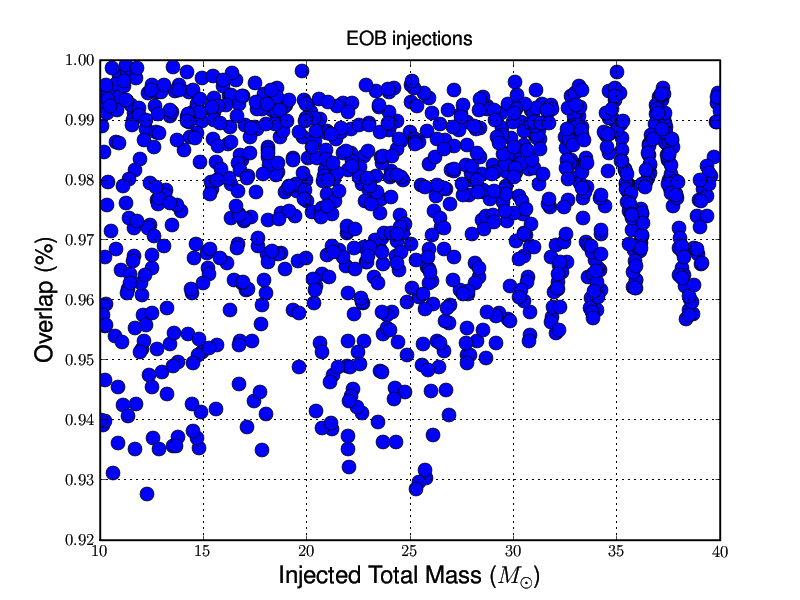
\includegraphics[width=0.4\textwidth]{bankefficiencydoc_snr_versus_totalmass.png}
\caption{\label{fig:snr1} Overlaps versus total mass}
\end{figure} 

Note that the XML table does not contains all the physical information you may want. It is quite light though because only 2 mass parameters are stored for the injection and for the btemplate that gives the best SNR. Indeed, other set of parameters can be computed a posteriori.

\subsection{Noise and Signal}\label{model}
In the two previous examples, we consider noiseless simulations. BankEfficiency was indeed created to check the overlap betweem a template bank and an injection. But, thanks to the noisemodel package, it is straightforward to use simulation where the signal is buried in some noise (you can even set the signal amplitude to be null so as to study only the noise).  This can be done as follows : 
\code{lalapps\_BankEfficiency {-}{-}template EOB {-}{-}signal EOB {-}{-}debug 33  {-}{-}mm 0.95 {-}{-}n 10000  {-}{-}xml-output {-}{-}print-bank  {-}{-}simulation-type NoiseAndSignal {-}{-}signal-amplitude 25}

The noise is a colored gaussian noise with a variance such that the average SNR is set by \textbf{{-}{-}signal-amplitude} to 25. 

This is very useful to perform test of the Fisher matrix by testing the dispersion/accuracy of the mass parameters. 

Usually, you would want the mass of the injection to be fixed instead  of being randomized. This can be done by fixing the individual masses as follows: 
\code{lalapps\_BankEfficiency {-}{-}template EOB {-}{-}signal EOB {-}{-}mm 0.95 {-}{-}n 10000  {-}{-}xml-output {-}{-}print-bank  {-}{-}simulation-type NoiseAndSignal {-}{-}signal-amplitude 25 {-}{-}m1 10 {-}{-}m2 10}

Another option related to the noise is that you may want to specify different type of colored noise, which currently are LIGOI, LIGOA, VIRGO, EGO, TAMA for initial LIGO, advanced LIGO, VIRGO, Einstein Telescope and TAMA, which can be fixed by \textbf{{-}{-}noise-model}.


\code{lalapps\_BankEfficiency {-}{-}template EOB {-}{-}signal EOB {-}{-}mm 0.95 {-}{-}n 10000  {-}{-}xml-output {-}{-}print-bank  {-}{-}simulation-type NoiseAndSignal {-}{-}signal-amplitude 25 {-}{-}m1 10 {-}{-}m2 10 {-}{-}noise-model LIGOA}

using the --print-psd option, the PSD will be saved in \textbf{BankEfficiency-PSD.dat}.

\subsection{template bank related}\label{bank}
Let us now look in more details at the parameters related to the template bank itself.

First of all, there are only two specific type of template bank available at the moment that are in the LAL bank package. The first template bank is the SPA template bank for physical modesl such as EOB,TAylor,Pade. The second one is a BCV template bank that is being called if \textbf{{-}{-}template} is set to \textbf{BCV}, which is discussed later on. Let us focus on the SPA template bank for now. 

There are two types of placement : square and hexagonal. Historically, square placement was implemented and can be called using \textbf{{-}{-}bank-grid-spacing SquareNotOriented}. Then hexagonal placement was imlemented and can be called using \textbf{{-}{-}bank-grid-spacing Hexagonal}

\textbf{Technical:}
A template bank is constructed using the metric components of the signal/template manifold. The metric components are computed by calculating quantities such as the  moments, whihc in turn are integrals from a lower cut-off frtequency to an upper cutoff frequency. The latter is  by default set to Nyquist frequency. One can force this upper cut-off frequency to be a fixed value by setting \textbf{{-}{-}bank-ffinal}. One can also recompute the moments for each template so that the upper cutoff frequency is the last stable orbit. This option is not et fully implemented but can be set on using \textbf{{-}{-}compute-moments} to recompoute the Gammas appropriately. 

By default the minimal match of the template bank is 80\% but you can change it using \textbf{{-}{-}mm} option.

To set the masse range to which the bank is efficient, use \textbf{{-}{-}bank-mass-range 1 3}.

There is also the possibility to create a template bank that has a fine grid. The fine grid is implemented within bankEfficiency and requires this parametres: 
\begin{itemize}
 \item \textbf{{-}{-}t0-fine-range} 2 values to set the t0 range
\item \textbf{{-}{-}t3-fine-range} 2 values to set the tau3 range
\item \textbf{{-}{-}t0-fine-bin} number of bins in this dimension
\item \textbf{{-}{-}t3-fine-bin} number of bins in this dimension
\end{itemize}



\subsection{Eccentricity related}\label{eccentricity}
If the signal is set to \textbf{Eccentricity} (using the {-}{-}signal option), then you can set the eccentricity of the simulated signals by using a range. The eccentricity will be uniformly distributed witin the two values that define this range. For instance :
\code{lalapps\_BankEfficiency {-}{-}template TaylorT3 {-}{-}signal Eccentricity {-}{-}mm 0.95 {-}{-}n 10000  {-}{-}xml-output --signal-eccentricity-range 0 0.4}

Note that the Eccentric model is only implemented at the Newtonian order for the moment. Therefore, one must specify the Newtonian order on the command line argument (by default the 2PN is used). If not, the code will fail. 

So, stricly speaking, the command above should have been : 
\code{lalapps\_BankEfficiency {-}{-}template TaylorT3 {-}{-}signal Eccentricity {-}{-}mm 0.95 {-}{-}n 10000  {-}{-}xml-output --signal-eccentricity-range 0 0.4 --signal-order 0}

where the number 0 stands for Newtonian.

There is no eccentric template bank. However, one can set the template bank to be based on SPA bank (optimised for a search that uses 2PN template) but place a eccentric template on each point of the grid. Yet, by default all template will have their eccentricity fixed to zero. So, really, this is not an eccentric template bank. To do so, one would need the metric in the eccentric dimension and create a template bank adequately. Yet, there is a naive template bank that is called by using the option \textbf{{}{}bank-eccentricity-range} followed by  a range of values and a number of bins. The template will be nbins times the original template bank each of them having a different value of eccentricity. This is naive because it assumes that the metric is flat in the eccentric dimension even though this is clearly not the case. However, one can already test how we can recover eccentric waveforms and performed some tests. 

\code{lalapps\_BankEfficiency {-}{-}template TaylorT3 {-}{-}signal Eccentricity {-}{-}mm 0.95 {-}{-}n 10000  {-}{-}xml-output --signal-eccentricity-range 0 0.4 --signal-order 0 --bank-eccentric-range 0 0.4 --bank-eccentricity-bins 10}

\subsection{BCV related functions}\label{bcv}
In this section, we show how to test a template bank based on BCV template and how a BCV template bank can detect signals based on other models such as EOB. 

First, the BCV template bank itself is set up using this arguments : 
--bank-alpha 0.01
--bank-psi0-range 10 250000
--bank-psi3-range -2200 -10
--bank-fcut 2 6
--bank-number-fcuts
--bank-inside-polygon

The BCV signal can be injected. We can force the psi0/psi values using --psi0 and -psi3 options. 
otherwise the --signal-psi0-range and --signal-psi3-range  need to be fixed or default values will be used instead.

Concerning the filtering there is an option to avoid the alpha constraint to be used --no-alpha-constraint --alpha-constraint



\subsection{Amplitude Corrected related}\label{ampcor}
To use the maplitude corrected waveforms, one can simply set the AmpCorPPN in --signal and --template. The order needs alos to be set by using --signal-amp-order  and --template-map-order

Concerning the input parameter of the signal, one also need to set the range of inclination and polarisation.  --signal-inclination-rane --signal-polarisation-range
Note however that because the signal are normalised with resepcte to their energy, the effect of the inclination on the amplitude of the signal wont be seen.

\subsection{others}\label{others}
There are a few other options. Some of whihc can be useful.
\subsubsection{force the length of the signal}
--num-seconds
\subsubsection{lower cut off}
--fl --fl-template  are equivalent and fix both the fl of the template and fl of the integration.

--fl-signal
\subsubsection{fast option}
--fast-simulation and --e-match 

\subsubsection{BHNS injection}
--bhns-injection

\subsubsection{check the code}
--check/faithfulness and --no-start-phase
--print-snr-histo

when --check is used, some parameters are not overwritten : flower, order, approximant,eccenticity,fFinal. only the mass parameetres. 
\section{Deploy your DAGs and CONDOR jobs}\label{dagandini}
\subsection{ini file}\label{ini}
\begin{verbatim}
[main]
executable=./lalapps_BankEfficiency

[general]
mm=0.95
sampling=2048
fl=40

[bank]
bank-grid-spacing=Hexagonal

[signal]
signal=EOB

[simulation]
ntrial=1000
njobs=100
\end{verbatim}

fix your ini file so that it does what you want.

\subsection{Generate the sub abd dag files.}\label{dag}
\code{python bep.py --config-file bep.ini}

\code{condor\_submit\_dag -maxjobs 100  -f bep.dag}


\section{Meaning of the bankefficiency XML table}\label{xml}
\begin{description}
\item[psi0] The first BCV parameter of the template
\item[psi3] The second BCV parameter of the template
\item[psi0\_sim] The first BCV parameter of the injection
\item[psi3\_sim] The second BCV parameter of the injection
\item[tau0] The first mass parameter of the template
\item[tau3] The second mass parameter of the template
\item[tau0\_sim] The first mass parameter of the injection
\item[tau3\_sim] The second mass parameter of the injection
\item[ecc] eccentricity of the best templates
\item[ecc\_sim] eccentricity of the signal
\item[ffinal] ffinal of the best templates
\item[ffinal\_sim] ffinal of the injection
\item[mass1\_sim] The first mass parameter of the injection
\item[mass2\_sim] The first mass parameter of the injection
\item[phase\_sim] The initial phase of the injection
\item[snr] the best overlap maximised over all template bank and time
\item[snr\_at\_ta] irrelevant for now
\item[phase] the phase of the best template
\item[alpha\_f] the alpha\_f value of the best template (BCV related)
\item[time] the time of arrival of the best template
\item[time\_sim] 
\item[nfast] number of templates really used
\end{description}

\section{Arguments and their default values}\label{default}
--bank-alpha 0.01\\
--bank-fcut-range\\
--bank-ffinal\\
--bank-inside-polygon\\
--bank-grid-spacing\\
--bank-number-fcut\\
--bank-mass-range 5 20\\
--bank-max-total-mass\\
--bank-min-total-mass\\
--bank-psi0-range 10 250000\\
--bank-psi3-range -2200 -10\\
--debug\\
--bank-eccentricity-range \\
--bank-eccentricity-bins\\ 
--e-match 0.5\\
--template-fl 40\\
--fl 40\\
--h\\
--ascii2xml\\
--m1\\
--m2\\
--mm 0.80\\
--ntrial 1\\
--noise-amplitude \\
--noise-model\\
--num-seconds\\
--psi0\\
--psi3\\
--sampling 2048\\
--seed\\
--signal EOB\\
--signal-alpha\\
--signal-amp-order\\
--signal-alpha1\\
--signal-alpha2\\
--signal-amplitude\\
--signal-eccentricity-range\\
--signal-ffinal\\
--signal-fl 40\\
--signal-inclination-range\\
--signal-polarisation-range\\
--signal-mass-range\\
--signal-tau0-range\\
--signal-tau3-range\\
--signal-order\\
--signal-nstartpad\\
--signal-psi0-range\\
--signal-psi3-range\\
--signal-random-nstartpad\\
--signal-max-total-mass\\
--signal-min-total-mass\\
--simulation-type\\
--t0-fine-range\\
--t3-fine-range\\
--t0-fine-bin\\
--t3-fine-bin\\
--no-start-phase\\
--tau0\\
--tau3\\
--template EOB\\
--template-order\\
--template-amp-order\\
--user-tag\\
--ambiguity\\
--alpha-constraint\\
--bhns-injection\\
--no-alpha-constraint\\
--print-best-overlap\\
--faithfulness\\
--check\\
--print-psd\\
--print-snr-histo\\
--verbose\\
--version\\
--print-bank\\
--compute-moments\\
--xml-output\\
--print-prototype\\
--fast-simulation\\

\section{FAQs}\label{faqs}
\subsection{Why BankEfficiency fails without any error message? }
Usually, the code is quite robust but there are a few places where it may fail. One is related to the size of the vectors not being long enough. By default we optimize the memory allocation by fixing the vector length to a minimal value. This value is estimated as twice the length of the longest template/signal to be used. If this estimation length is not done properly, when a signal is generated and overtakes this length, the program will fail.

An other reason could be related to the PN order not being set properly.

Usually, with a segmentation fault, this is related to vecrtor not being set properly.


% bibliography : bank papers : square, hexa, bcvspin, S3SBBH, reinhard, owen, Sathya,
\begin{thebibliography}{99}
\bibitem{LIGO}
A. Abramovici {\it et al.}, Science {\bf 256}, 325 (1992);
B. Abbott, {\it et al.}, Nuclear Inst. and Methods in Physics 
Research, A {\bf 517/1-3} 154 (2004).

\bibitem{VIRGO}
B. Caron {\it et al.}, Class. Quantum Grav. {\bf 14}, 1461 (1997);
F. Acernese {\it et al.}, {\em The Virgo detector,} 
Prepared for 17th Conference on High Energy Physics (IFAE 2005) (In Italian), 
Catania, Italy, 30 Mar-2 Apr 2005,  AIP Conf. Proc. {\bf 794}, 307-310 (2005).

\bibitem{damir}
F.~Beauville et al, Class.\ Quant.\ Grav.\ \textbf{22}, 4285, (2005).

\bibitem{Owen96}B.~Owen, Phys.\ Rev.\  D\textbf {53}, 6749 (1996).

\bibitem{OwenSathyaprakash98} B.~Owen, B.~S.~Sathyaprakash 1998 Phys.\ Rev.\ 
D \textbf{60} 022002 (1998).

\bibitem{squarebank}
S.~Babak and R.~Balasubramanian and D.~Churches and T.~Cokelaer and B.~S.~Sathyaprakash 2006 \textit{Class.\ Quantum Grav.\ }
\textbf{23} 5477

\bibitem{hexabank} T.~Cokelaer 2007 \textit{Gravitational Wave Detections of Inspiralling Compact Binaries: Hexagonal Template Placement and Physical Template Families}, (\textit{Preprint} gr-qc/0706.4437v1), Phys. Review D 76, 10, 2007 (15 Nov 2007) 


\bibitem{bcvbank} T.Cokelaer, 2007, \textit{A template bank to search for gravitational waves from inspiralling compact binaries: II. Phenomenological model}
Class. Quantum Grav. 24 (2007) 6227-6242 


\bibitem{BDI95} L. Blanchet, T. Damour and B.R. Iyer, Phys.\ Rev.\ D {\bf 51},5360 (1995).

\bibitem{LAL} LSC Algorithm Library LAL,\\
{\tt http://www.lsc-group.phys.uwm.edu/daswg/\-projects/lal.html}

\bibitem{LIGOS3S4}
B.~Abbott {\it et al.}, LIGO Scientific Collaboration, gr-qc/0704.3368v2,
(2007)

\bibitem{PSDs}
T.~Damour and B.R.~Iyer and B.S.~Sathyaprakash, Phys.\ Rev.\ D
\textbf{63}, 044023 (2001).

\end{thebibliography}


\label{theend}

\end{document}          


%\clearpage
%\subsection{Program \texttt{lalapps\_BankNumberOfTemplates}}
\label{program:lalapps-BankNumberOfTemplates}
\idx[Program]{lalapps\_BankNumberOfTemplates}
{\LARGE{{\bf Documentation In progress}}}

\begin{entry}

\item[Name]
\verb$lalapps_BankNumberOfTemplates$ --- Compute the number of templates given 
by a bank.

\item[Synopsis]
\verb$lalapps_BankNumberOfTemplates$ [\verb$-h$] 
[\verb$--alpha-range$   \textit{$\alpha_{Min}$}\texttt{\&}\textit{$\alpha_{Max}$}]
[\verb$--d-range$   \textit{step in $\alpha$}]
[\verb$--fend-bcv$     \textit{$f_{cut}Min$}\texttt{\&}\textit{$f_{cut}Max$}]
[\verb$--fl$	\textit{lower cutoff frequency}]
[\verb$--mm$ \textit{MinimalMatch}]
[\verb$--number-fcut$ \textit{number of layers } \textit{ in $f_{cut}$ dimension}]
[\verb$--psi0-range$ \textit{$\psi0_{Min}$}\texttt{\&}\textit{$\psi0_{Max}$}]
[\verb$--psi3-range$ \textit{$\psi3_{Min}$}\texttt{\&}\textit{$\psi3_{Max}$}]







\item[Description]
\verb$lalapps_BankNumberOfTemplates$ This application compute the number of 
templates in  a bank of templates based on the SPA bank or BCV bank.

To compute the number of templates one need the minimal match, the lower cutoff
frequency and a range of parameters such as masses or $\tau_i$ in the SPA case or 
$\psi_0$ and $\psi_3$ in the  BCV case. 

Concerning BCV, we also need the alpha parameter. 

In the BCV case, a range of alpha value is given [0-1] by default as well as a step
 (0.01 by default). Thus it provides an easy way to see the evolution of the number of
templates with respect to the $\alpha$ parameter. 

Later, we might add options to do the same but with a range in the lower frequency for
instance.


\item[Options related to the simulations]\leavevmode
\begin{entry}
\item[\texttt{--alpha-range}]
alpha parameter to compute the metric.
\item[\texttt{--dalpha}]
step in alpha parameter.
\item[\texttt{--fend-bcv}]
Range of cutoff frequency for the BCV template creation. User must provide two parameters: 
the lowest and upper frequency cutoff. Those frequency are not expressed in Hz but in term
of distance betwwen the two objets. for instance at the last stable orbit, the distance 
between the two objects is 6GM. In the case of an EOB description, the distance between 
the two objects is closer to 3GM. A good compromise is to use fend-bcv between 8GM and 3GM
and using the options --number-fcut = 5. 
\item[\texttt{-h}]
Print a help message.
\item[\texttt{--mm}]
Fixe the Minimal Match of the bank.
\item[\texttt{--n}]
Number of trials, i.e number of injections.
\item[\texttt{--number-fcut}]
Number of layers to create in the BCV bank in the fend-bcv dimension. 
Given the lower and upper frequency (see option fend-bcv), the bank creates
n layers each of them having a frequency between lowest fend-bcv and highest fend-bcv.
\item[\texttt{--psi0-range}]
Range of paramter psi0. User must give two positive numbers.
\item[\texttt{--psi3-range}]
Range of paramter psi3. User must give two negative numbers.
\item[\texttt{--seed}]
Random seed.
\item[\texttt{--space}]
When --bank is given we should also provide the space of parameter. In the case
of a BCV bank is it Psi0Psi3 and there is only one space. But in the SPA case on 
might provide either Tau0Tau3 or Tau0Tau2 option. 

\end{entry}


\item[EXAMPLE]
\begin{verbatim}
lalapps_BankNumberOfTemplates --dalpha 0.001 --alpha-range 0 1 
 --bank BCV

lalapps_BankNumberOfTemplates  --bank SPA --space Tau0Tau3
\end{verbatim}
\item[Author]
Thomas Cokelaer

\end{entry}


\chapter{Package \texttt{ring}}

\newpage\input{RingH}
\newpage\input{LALRingDownH}
\newpage\input{LALWienerH}

\newpage\begin{thebibliography}{0}
\bibitem{EWLeaver}
  E. W. Leaver, Proc. R. Soc. London \textbf{A402}, 285 (1985).
\bibitem{FEcheverria}
  F. Echeverria, Phys. Rev. D \textbf{40}, 3194 (1989).
\bibitem{BJOwen}
  B. J. Owen, Phys. Rev. D \textbf{53}, 6749 (1996).
\bibitem{JDECreighton}
  J. D. E. Creighton, Phys. Rev. D \textbf{60}, 022001 (1999).
\end{thebibliography}


\section{Stochastic Search Programs}
\label{section:stochastic}

This section of \textsc{LALApps} contains programs that can be used to
search interferometer data for stochastic gravitational wave
backgrounds.

\clearpage
\section{Program \texttt{lalapps\_olapredfcn}}
\label{program:lalapps-olapredfcn}
\idx[Program]{lalapps\_olapredfcn}

\begin{entry}

\item[Name]
%
  \verb$lal_olapredfcn$ --- computes overlap reduction function given
  a pair of known detectors.

\item[Synopsis]
%
  \verb$lal_olapredfcn $[\verb$-h$]\verb$ $[\verb$-q$]\verb$ $[\verb$-v$]
  \verb$ $[\verb$-d debugLevel $]\verb+ \+\newline
  \verb$   $
  \verb$-s siteID1 $[\verb$-a azimuth1$]
  \verb$-t siteID2 $[\verb$-b azimuth2$]\verb+ \+\newline
  \verb$   $
  [\verb$-f fLow$]\verb$ -e deltaF$\verb$ -n numPoints$\verb$ -o outfile$
                         
\item[Description]
%
  \verb$lal_olapredfcn$ computes the overlap reduction function
  $\gamma(f)$ for a pair of known gravitational wave detectors.  It
  uses the LAL function \verb$LALOverlapReductionFunction()$, which is
  documented in the LAL Software Documentation under the
  \texttt{stochastic} package.

\item[Options]\leavevmode
\begin{entry}
\item[\texttt{-h}]
  Print a help message.
\item[\texttt{-q}]
  Run silently (redirect standard input and error to \texttt{/dev/null}).
\item[\texttt{-v}]
  Run in verbose mode.
\item[\texttt{-d} \textit{debugLevel}]
  Set the LAL debug level to \textit{debugLevel}.
\item[\texttt{-s} \textit{siteID1} \texttt{-t} \textit{siteID2}]
  Use detector sites identified by \textit{siteID1} and
  \textit{siteID2}; ID numbers between \texttt{LALNumCachedDetectors}
  (defined in the \texttt{tools} package of LAL) refer to detectors
  cached in the constant array \verb$lalCachedDetectors[]$.  (At this
  point, these are all interferometers.)  Additionally, the five
  resonant bar detectors of the IGEC collaboration can be specified.
  The bar geometry data (summarized in table~\ref{table:cachedBars})
  is used by the fucntion \verb$LALCreateDetector()$ from the
  \texttt{tools} package of LAL to generate the Cartesian position
  vector and response tensor which are used to calculate the overlap
  reduction function.  The ID numbers for the bars depend on the value
  of \texttt{LALNumCachedDetectors}; the correct ID numbers can be
  obtained by with the command
\begin{verbatim}
./lalapps_olapredfcn -h
\end{verbatim}
\item[\texttt{-a} \textit{azimuth1} \texttt{-b} \textit{azimuth2}]
%
  If \textit{siteID1} (\textit{siteID2}) is a bar detector, assume it
  has an azimuth of \textit{azimuth1} (\textit{azimuth2}) degrees East
  of North rather than the default IGEC orientation given in
  table~\ref{table:cachedBars}.  Note that this convention, measuring
  azimuth in degrees clockwise from North is not the same as that used
  in LAL (which comes from the frame spec).  Note also that any
  specified azimuth angle is ignored if the corresponding detector is
  an interferometer.
\item[\texttt{-f} \textit{fLow}]
  Begin the frequency series at a frequency of \textit{fLow}\,Hz; if this
  is omitted, the default value of 0\,Hz is used.
\item[\texttt{-e} \textit{deltaF}]
  Construct the frequency series with a frequency spacing of
  \textit{deltaF}\,Hz
\item[\texttt{-n} \textit{numPoints}]
  Construct a frequency series with \textit{numPoints} points.
\item[\texttt{-o} \textit{outfile}]
  Write the output to file \textit{outfile}.  The format of this file
  is that output by the routine \verb$LALPrintFrequencySeries()$ in
  the \texttt{support} package of LAL, which consists of a header
  describing metadata followed by two-column rows, each containing the
  doublet $\{f,\gamma(f)\}$.
\end{entry}

\begin{table}[tbp]
  \begin{center}
    \begin{tabular}{|c|c|c|c|}
\hline
      Name & Longitude & Latitude & Azimuth
\\ \hline
\verb$AURIGA$ & $11^\circ56'54''$E & $45^\circ21'12''$N & N$44^\circ$E 
\\ \hline
\verb$NAUTILUS$ & $12^\circ40'21''$E & $41^\circ49'26''$N & N$44^\circ$E 
\\ \hline
\verb$EXPLORER$ & $6^\circ12'$E & $46^\circ27'$N & N$39^\circ$E 
\\ \hline
\verb$ALLEGRO$ & $91^\circ10'43.\!\!''766$W & $30^\circ24'45.\!\!''110$N 
& N$40^\circ$W
\\ \hline
\verb$NIOBE$ & $115^\circ49'$E & $31^\circ56'$S & N$0^\circ$E 
\\ \hline
    \end{tabular}
    \caption{Location and orientation data for the five IGEC resonant
      bar detectors, stored in the \texttt{lalCachedBars[]}
      array.  The data are taken from
      \texttt{http://igec.lnl.infn.it/cgi-bin/browser.pl?Level=0,3,1}
      except for the latitude and longitude of ALLEGRO, which were
      taken from Finn \& Lazzarini, gr-qc/0104040.  Note that the
      elevation above the WGS-84 reference ellipsoid and altitude
      angle for each bar is not given, and therefore set to zero.}
    \label{table:cachedBars}
  \end{center}
\end{table}


\item[Example usage]
  To compute the overlap reduction function for LIGO Hanford and
  LIGO Livingston, with a resolution of 1\,Hz from 0\,Hz to 1024\,Hz:
\begin{verbatim}
lalapps_olapredfcn -s 0 -t 1 -e 1 -n 1025 -o LHOLLO.dat
\end{verbatim}
  
  To compute the overlap reduction function for ALLEGRO in its optimal
  orientation of $72.\!\!^\circ08$ West of South (see Finn \& Lazzarini,
  gr-qc/0104040) and LIGO Livingston, with a resolution of 0.5\,Hz from
  782.5\,Hz to 1032\,Hz (assuming \texttt{lalNumCachedBars} is 6):
\begin{verbatim}
lalapps_olapredfcn -s 9 -a 252.08 -t 1 -f 782.5 -e 0.5 -n 500 -o ALLEGROLHO.dat
\end{verbatim}

\item[Author]
John T.~Whelan

\end{entry}


\clearpage
\subsection{Program \texttt{lalapps\_stochastic\_pipe}}
\label{program:stochastic-pipeline}
\idx[Program]{stochastic\_pipeline.py}

\begin{entry}
\item[Name]
\verb$lalapps_stochastic_pipe$ --- python script to generate Condor DAGs
to run the stochastic pipeline.

\item[Synopsis]
\begin{verbatim}
  -h, --help               display this message
  -v, --version            print version information and exit

  -d, --datafind           run LSCdataFind to create frame cache files
  -s, --stochastic         run lalapps_stochastic

  -p, --playground-only    only create chunks that overlap with playground
  -P, --priority PRIO      run jobs with condor priority PRIO

  -f, --config-file FILE   use configuration file FILE
  -l, --log-path PATH      directory to write condor log file
\end{verbatim}

\item[Description] \verb$lalapps_stochastic_pipe$ generates a Condor DAG
to run the stochastic search pipeline. The configuration should specify
the parameters needed to run the jobs and must be specified with the
\verb$--config-file$ option. A file containing science segments to
analysed should be specified in the \verb$[input]$ section of the
configuration file with a line such as
\begin{verbatim}
segments = S2H1L1v03_selectedsegs.txt
\end{verbatim}
This should contain four whitespace separated columns:
\begin{verbatim}
  segment_id    gps_start_time    gps_end_time    duration
\end{verbatim}
that define the science segments to be used. Lines starting with an
octothorpe are ignored.

\item[Example]
Generate a DAG to run a stochastic search on a pair of interferometers
specified in the configuration file. The generated DAG is then submitted
with \texttt{condor\_submit\_dag}
\begin{verbatim}
lalapps_inspiral_pipe --log-path /home/ram/dag_logs \
--datafind --stochastic --config-file stochastic_H1L1.ini

condor_submit_dag stochastic_H1L1.dag
\end{verbatim}

\item[Author]
Adam Mercer
\end{entry}

\clearpage
\subsection{Program \texttt{lalapps\_stochastic}}
\label{program:lalapps-stochastic}
\idx[Program]{lalapps\_stochastic}

\begin{entry}
\item[Name]
\verb$lalapps_stochastic$ --- standalone stochastic analysis code.

\item[Synopsis]
\begin{verbatim}
 --help                        print this message
 --version                     display version
 --verbose                     verbose mode
 --debug-level LEVEL           set lalDebugLevel
 --gps-start-time SEC          GPS start time
 --gps-end-time SEC            GPS end time
 --segment-duration SEC        segment duration
 --resample-rate F             resample rate
 --f-min F                     minimal frequency
 --f-max F                     maximal frequency
 --hann-duration SEC           hann duration
 --ifo-one IFO                 ifo for first stream
 --ifo-two IFO                 ifo for second stream
 --data-cache-one FILE         cache file for first stream
 --data-cache-two FILE         cache file for second stream
 --calibration-cache-one FILE  first stream calibration cache
 --calibration-cache-two FILE  second stream calibration cache
 --apply-mask                  apply frequency masking
 --inject                      inject a signal into the data
 --scale-factor N              scale factor for injection
 --seed N                      seed
 --overlap-hann                overlaping hann windows for data windowing
 --high-pass-filter            perform high pass filtering
\end{verbatim}

\item[Description] \verb$lalapps_stochastic$ runs the standalone
stochastic analysis code.

\item[Author] 
Adam Mercer, Tania Regimbau
\end{entry}


\backmatter

\nocite{*}
\bibliography{lalapps}

\printindex

\end{document}
